\documentclass{article}

\usepackage{packages}
\usepackage{environments}
\usepackage{commands}

\begin{document}

\title{Лекции по Линейной Алгебре}
\author{Дима Трушин}
\date{2023 --- 2024}
	
\maketitle
\tableofcontents

\ProvidesFile{lecture01.tex}[Лекция 1]

\newpage

\section{Системы линейных уравнений}

\subsection{Системы линейных уравнений и связанная с ними терминология}

Наша задачи научиться решать Системы Линейных Уравнений (СЛУ), то есть находить все их решения или доказывать, что решений нет.
Общий вид СЛУ и ее однородная версия (ОСЛУ):
\[
\left\{
\begin{aligned}
a_{11}x_1 + &\ldots + a_{1n}x_n = b_1\\
&\ldots \\
a_{m1}x_1 + &\ldots + a_{mn}x_n = b_m
\end{aligned}
\right.\quad\quad
\left\{
\begin{aligned}
a_{11}x_1 + &\ldots + a_{1n}x_n = 0\\
&\ldots \\
a_{m1}x_1 + &\ldots + a_{mn}x_n = 0
\end{aligned}
\right.
\]

\paragraph{Коэффициенты}

Где живут коэффициенты $a_{ij}$ и $b_j$?
Варианты:
\begin{itemize}
\item Вещественные числа $\mathbb R$

\item Комплексные числа $\mathbb C$

\item Рациональные числа $\mathbb Q$
\end{itemize}
Для решения СЛУ {\bf НЕ} имеет значения откуда берутся коэффициенты, так как решения будут лежать там же.
Главное, чтобы для коэффициентов были определены операции сложения, вычитания, умножения и деления.%
\footnote{Позже мы введем понятие поля и допустимыми будут коэффициенты из произвольного поля.}
Потому мы будем работать с числами из $\mathbb R$.
А вот целые числа $\mathbb Z$ уже не подходят, так как в них нельзя делить.

\paragraph{Решение}

Решением системы линейных уравнений называется набор чисел $(c_1,\ldots,c_n)$, $c_i\in\mathbb R$ такой, что при подстановке $c_i$ вместо $x_i$, все уравнения системы превращаются в верные равенства.
Введем обозначение $\mathbb R^n = \mathbb R\times \ldots \times \mathbb R = \{(c_1,\ldots,c_n)\mid c_i\in \mathbb R\}$.
То есть элемент $\mathbb R^n$ -- это набор из $n$ вещественных чисел.
Потому любое решение $c=(c_1,\ldots,c_n)$ является элементом $\mathbb R^n$.

\subsection{Матрицы связанные со СЛУ}

Для каждой СЛУ введем следующие обозначения:
\[
A= 
\begin{pmatrix}
a_{11}&\ldots& a_{1n}\\
\vdots&\ddots&\vdots\\
a_{m1}& \ldots &a_{mn}
\end{pmatrix}\quad
b = 
\begin{pmatrix}
b_1\\
\vdots\\
b_m
\end{pmatrix} \quad
x =
\begin{pmatrix}
x_1\\
\vdots\\
x_n
\end{pmatrix}\quad
(A|b) =
\left(\left.
\begin{matrix}
a_{11}&\ldots&a_{1n}\\
\vdots&\ddots&\vdots\\
a_{m1}&\ldots&a_{mn}\\
\end{matrix}
\:\right|\:
\begin{matrix}
b_1\\
\vdots\\
b_m\\
\end{matrix}\right)
\]
Названия:
\begin{itemize}
\item $A$ -- матрица системы

\item $b$ -- вектор правой части

\item $(A|b)$ -- расширенная матрица системы

\item $x$ -- вектор решений
\end{itemize}
Будем кратко записывать СЛУ и ее однородную версию так: $Ax = b$ и $Ax = 0$.
Также для краткости будем обозначать системы буквами $\Sigma$.

При решении системы линейных уравнений приходится помногу раз переписывать кучу данных.
Для того чтобы сократить эти записи, целесообразно сократить количество записываемой на бумаге информации.
Расширенная матрица системы $(A|b)$ является необходимым минимумом такой информации.
Потому сейчас к такой записи можно относиться как к удобному способу компактно записать систему.

\paragraph{Количество решений}

Случай одного уравнения и одной неизвестной $ax = b$, где $a, b\in \mathbb R$:
\begin{itemize}
\item При $a\neq 0$ -- одно решение $x = b/a$.

\item При $a = 0$, $b\neq 0$ -- нет решений.

\item При $a = 0$, $b = 0$ -- любое число является решением, т.е. бесконечное число решений.
\end{itemize}

\paragraph{Что значит решить систему}

Обычно принято говорить следующие слова: решить систему значит описать множество ее решений, то есть либо доказать, что система не имеет решений вовсе, либо описать все наборы, которые являются решениями.
Если система не имеет решений, она называется {\it несовместной}, в противном случае -- {\it совместной}.
Однако, в этой фразе не понятно, что имеется в виду.
Действительно, если я запишу систему
\[
\left\{
\begin{aligned}
x + 2 y + 3z &= 0\\
4x + 5y + 6z &= 0\\
7x + 8y + 9z &= 0
\end{aligned}
\right.
\]
То я могу описать множество решений словами: это все наборы $(x, y, z)$ подходящие под систему.
Это звучит как жульничество, тем не менее в этом описании есть содержательная мысль, давайте я ее озвучу явно.
Приведенная выше система позволяет нам быстро решать такую задачу: проверить лежит ли данный набор среди решений.
То есть мы эффективно умеем тестировать вопрос на принадлежность множеству решений.
Однако, такое описание не позволяет решать другую важную задачу: генерировать все решения по одному разу.
То есть, глядя на эту систему, вы вряд ли сходу предъявите набор отличный от $(0, 0, 0)$ в качестве решения.
Более того, тут даже не понятно, есть ли какие-то другие наборы или нет.
Потому мы хотим найти другое описание множества решений, которое бы позволяло быстро решать обе задачи: и задачу принадлежности и задачу генерации.
Оказывается, что это тоже делается с помощью систем, только в очень специальном виде.

\paragraph{Эквивалентные системы}

Пусть даны две системы линейных уравнений с одинаковым числом неизвестных (но быть может разным числом уравнений) $\Sigma_1$ и $\Sigma_2$.
Будем говорить, что эти системы эквивалентны и писать $\Sigma_1 \sim \Sigma_2$, если множества решений этих систем совпадают.
Если $E_i\subseteq \mathbb R^n$ -- множество решений $i$-ой системы, то системы эквивалентны, если $E_1 = E_2$.

Вот полезный пример эквивалентных систем:
\[
\left\{
\begin{aligned}
x + y &= 1\\
x - y &= 0
\end{aligned}
\right.\quad\sim\quad
\left\{
\begin{aligned}
2x &= 1\\
2y &= 1
\end{aligned}
\right.
\]

\paragraph{Как решать систему}

Пусть нам надо решить систему $\Sigma$.
Идея состоит в том, чтобы постепенно менять ее на эквивалентную до тех пор, пока она не упростится до такого состояния, что все ее решения легко описать.
\[
\Sigma = \Sigma_1 \mapsto \Sigma_2 \mapsto \ldots \mapsto \Sigma_n \leftarrow\text{ легко решается}
\]
Теперь надо объяснить две вещи: (1) какого сорта преобразования над системами мы будем делать и (2) к какому замечательному виду мы их приводим и как в нем выглядят все решения.
Ответам на эти два вопроса и будет посвящена оставшаяся часть лекции.

\subsection{Элементарные преобразования} 

Мы разделим все преобразования на три типа%
\footnote{Стоит отметить, что нумерация типов преобразования не является общепринятой и отличается от учебника к учебнику.}:
\begin{align*}
\text{I тип: }&
\left(\left.
\begin{matrix}
a_{11}&\ldots&a_{1n}\\
a_{i1}&\ldots&a_{in}\\
a_{j1}&\ldots&a_{jn}\\
a_{m1}&\ldots&a_{mn}
\end{matrix}
\:\right|\:
\begin{matrix}
b_1\\
b_i\\
b_j\\
b_m
\end{matrix}
\right)
\mapsto
\left(\left.
\begin{matrix}
a_{11}&\ldots&a_{1n}\\
a_{i1}&\ldots&a_{in}\\
a_{j1} + \lambda a_{i1}&\ldots&a_{jn}+ \lambda a_{in}\\
a_{m1}&\ldots&a_{mn}
\end{matrix}
\:\right|\:
\begin{matrix}
b_1\\
b_i\\
b_j+ \lambda b_i\\
b_m\\
\end{matrix}
\right)
\quad i\neq j
\\
\text{II тип: }&
\left(\left.
\begin{matrix}
a_{11}&\ldots&a_{1n}\\
a_{i1}&\ldots&a_{in}\\
a_{j1}&\ldots&a_{jn}\\
a_{m1}&\ldots&a_{mn}
\end{matrix}
\:\right|\:
\begin{matrix}
b_1\\
b_i\\
b_j\\
b_m
\end{matrix}
\right)
\mapsto
\left(\left.
\begin{matrix}
a_{11}&\ldots&a_{1n}\\
a_{j1}&\ldots&a_{jn}\\
a_{i1}&\ldots&a_{in}\\
a_{m1}&\ldots&a_{mn}
\end{matrix}
\:\right|\:
\begin{matrix}
b_1\\
b_j\\
b_i\\
b_m
\end{matrix}
\right)
\\
\text{III тип: }&
\left(\left.
\begin{matrix}
a_{11}&\ldots&a_{1n}\\
a_{i1}&\ldots&a_{in}\\
a_{m1}&\ldots&a_{mn}
\end{matrix}
\:\right|\:
\begin{matrix}
b_1\\
b_i\\
b_m
\end{matrix}
\right)
\mapsto
\left(\left.
\begin{matrix}
a_{11}&\ldots&a_{1n}\\
\lambda a_{i1}&\ldots&\lambda a_{in}\\
a_{m1}&\ldots&a_{mn}
\end{matrix}
\:\right|\:
\begin{matrix}
b_1\\
\lambda b_i\\
b_m
\end{matrix}
\right)
\quad \lambda \neq 0
\end{align*}
Поясним словами, что делают преобразования:
\begin{enumerate}
\item Прибавляем к $j$-ой строке $i$-ю, умноженную на константу $\lambda\in\mathbb R$.

\item Меняем местами $i$-ю и $j$-ю строки.

\item Умножаем $i$-ю строку на ненулевую константу $\lambda\neq 0$, $\lambda\in \mathbb R$.
\end{enumerate}

\subsection{Алгоритм Гаусса}

Этот метод заключается в приведении СЛУ к некоторому <<ступенчатому виду>>, где множество решений очевидно.%
\footnote{Данный метод является самым быстрым возможным как для написания программ, так и для ручного вычисления.
При вычислениях руками, однако, полезно местами пользоваться <<локальными оптимизациями>>, то есть если вы видите, что какая-то хитрая комбинация строк сильно упростит вид системы, то сделайте ее.}
Разберем типичный ход алгоритма Гаусса на примере $3$ уравнений и $4$ неизвестных.%
\footnote{При переходе от одной матрицы к другой я новым коэффициентам даю старые имена, чтобы не захламлять текст новыми обозначениями.}

\paragraph{Прямой ход алгоритма Гаусса}

Идея прямого хода алгоритма в следующем.
Мы смотрим на левый верхний элемент в матрице и пытаемся с помощью него обнулить все элементы под ним.
Как только обнулили, забываем про первую строку и столбец и повторяем процедуру с оставшейся подматрицей.
\begin{align*}
\left(\left.
\begin{matrix}
a_{11}& a_{12}&a_{13}& a_{14}\\
a_{21}& a_{22}&a_{23}& a_{24}\\
a_{31}& a_{32}&a_{33}& a_{34}\\
\end{matrix}
\:\right|\:
\begin{matrix}
b_1\\
b_2\\
b_3\\
\end{matrix}
\right)&
\quad 2\text{-я строка }-\frac{a_{21}}{a_{11}}\cdot1\text{-я строка}\quad\\
\left(\left.
\begin{matrix}
a_{11}& a_{12}&a_{13}& a_{14}\\
0& a_{22}&a_{23}& a_{24}\\
a_{31}& a_{32}&a_{33}& a_{34}\\
\end{matrix}
\:\right|\:
\begin{matrix}
b_1\\
b_2\\
b_3\\
\end{matrix}
\right)&
\quad 3\text{-я строка }-\frac{a_{31}}{a_{11}}\cdot1\text{-я строка}\quad\\
\left(\left.
\begin{matrix}
a_{11}& a_{12}&a_{13}& a_{14}\\
0& a_{22}&a_{23}& a_{24}\\
0& a_{32}&a_{33}& a_{34}\\
\end{matrix}
\:\right|\:
\begin{matrix}
b_1\\
b_2\\
b_3\\
\end{matrix}
\right)&
\quad 3\text{-я строка }-\frac{a_{32}}{a_{22}}\cdot2\text{-я строка}\quad\\
\left(\left.
\begin{matrix}
a_{11}& a_{12}&a_{13}& a_{14}\\
0& a_{22}&a_{23}& a_{24}\\
0& 0&a_{33}& a_{34}\\
\end{matrix}
\:\right|\:
\begin{matrix}
b_1\\
b_2\\
b_3\\
\end{matrix}
\right)&
\end{align*}
В рассуждениях выше, мы пользовались тем, что угловые элементы $a_{11}$ и $a_{22}$ не нули.
Но вообще говоря так могло не получиться.
Например на третьем шаге могла быть одна из следующих ситуаций (здесь мы смотрим на элемент $a_{22}$):
\[
\left(\left.
\begin{matrix}
a_{11}& a_{12}&a_{13}& a_{14}\\
0&0&a_{23}& a_{24}\\
0& a_{32}&a_{33}& a_{34}\\
\end{matrix}
\:\right|\:
\begin{matrix}
b_1\\
b_2\\
b_3\\
\end{matrix}
\right)
\quad\text{или}\quad
\left(\left.
\begin{matrix}
a_{11}& a_{12}&a_{13}& a_{14}\\
0& 0&a_{23}& a_{24}\\
0& 0&a_{33}& a_{34}\\
\end{matrix}
\:\right|\:
\begin{matrix}
b_1\\
b_2\\
b_3\\
\end{matrix}
\right)
\]
В первом случае $a_{22} = 0$, но при этом есть какой-то ненулевой элемент под ним.
В такой ситуации надо переставить вторую строчку с другой строкой, где второй элемент не ноль.
В примере надо переставить вторую и третью строчку местами.
Во втором случае $a_{22} = 0$ и все элементы под ним.
В такой ситуации надо пропустить второй столбец и перейти к третьему и мы смотрим на элемент $a_{23}$.
После чего повторяем алгоритм Гаусса с подматрицей.

В результате прямого хода алгоритма из-за обнуления коэффициентов могут возникнуть следующие случаи%
\footnote{Это не полный список всех случаев.}
\[
\left(\left.
\begin{matrix}
\underline{a_{11}}& a_{12}&a_{13}& a_{14}\\
0& \underline{a_{22}}&a_{23}& a_{24}\\
0& 0&0& \underline{a_{34}}\\
\end{matrix}
\:\right|\:
\begin{matrix}
b_1\\
b_2\\
b_3\\
\end{matrix}
\right)
\quad
\left(\left.
\begin{matrix}
\underline{a_{11}}& a_{12}&a_{13}& a_{14}\\
0& 0&\underline{a_{23}}& a_{24}\\
0& 0&0& \underline{a_{34}}\\
\end{matrix}
\:\right|\:
\begin{matrix}
b_1\\
b_2\\
b_3\\
\end{matrix}
\right)
\quad
\left(\left.
\begin{matrix}
\underline{a_{11}}& a_{12}&a_{13}& a_{14}\\
0& \underline{a_{22}}&a_{23}& a_{24}\\
0& 0&0& 0\\
\end{matrix}
\:\right|\:
\begin{matrix}
b_1\\
b_2\\
\underline{b_3}\\
\end{matrix}
\right)
\quad
\left(\left.
\begin{matrix}
\underline{a_{11}}& a_{12}&a_{13}& a_{14}\\
0& \underline{a_{22}}&a_{23}& a_{24}\\
0& 0&0& 0\\
\end{matrix}
\:\right|\:
\begin{matrix}
b_1\\
b_2\\
0\\
\end{matrix}
\right)
\]

\paragraph{Главные и неглавные переменные}

Подчеркнутые элементы считаются не равными нулю.
Это первые ненулевые коэффициенты в строке, они называются лидерами.
В ступенчатом виде все переменные делятся на главные и свободные.
Соответствующие лидерам переменные называются главными.
Остальные переменные называются свободными.

\paragraph{Обратный ход алгоритма Гаусса}

Задача обратного хода алгоритма в том, чтобы сделать все лидирующие коэффициенты единицами, а все коэффициенты над ними обнулить.
Обратный ход осуществляется снизу вверх.
Разберем типичный обратный ход алгоритма Гаусса.
Подчеркнутые элементы считаются не равными нулю.
\begin{align*}
\left(\left.
\begin{matrix}
\underline{a_{11}}& a_{12}&a_{13}& a_{14}\\
0& \underline{a_{22}}&a_{23}& a_{24}\\
0& 0&\underline{a_{33}}& a_{34}\\
\end{matrix}
\:\right|\:
\begin{matrix}
b_1\\
b_2\\
b_3\\
\end{matrix}
\right)&
\quad \text{разделить }i\text{-ю строку на }a_{ii}\\
\left(\left.
\begin{matrix}
1& a_{12}&a_{13}& a_{14}\\
0& 1&a_{23}& a_{24}\\
0& 0&1& a_{34}\\
\end{matrix}
\:\right|\:
\begin{matrix}
b_1\\
b_2\\
b_3\\
\end{matrix}
\right)&
\quad 2\text{-я строка }-a_{23}\cdot3\text{-я строка}\\
\left(\left.
\begin{matrix}
1& a_{12}&a_{13}& a_{14}\\
0& 1&0& a_{24}\\
0& 0&1& a_{34}\\
\end{matrix}
\:\right|\:
\begin{matrix}
b_1\\
b_2\\
b_3\\
\end{matrix}
\right)&
\quad 1\text{-я строка }-a_{13}\cdot3\text{-я строка}\\
\left(\left.
\begin{matrix}
1& a_{12}&0& a_{14}\\
0& 1&0& a_{24}\\
0& 0&1& a_{34}\\
\end{matrix}
\:\right|\:
\begin{matrix}
b_1\\
b_2\\
b_3\\
\end{matrix}
\right)&
\quad 1\text{-я строка }-a_{12}\cdot2\text{-я строка}\\
\left(\left.
\begin{matrix}
1& 0&0& a_{14}\\
0& 1&0& a_{24}\\
0& 0&1& a_{34}\\
\end{matrix}
\:\right|\:
\begin{matrix}
b_1\\
b_2\\
b_3\\
\end{matrix}
\right)&
\end{align*}
В специальных случаях приведенных выше, получим
\[
\left(\left.
\begin{matrix}
1& 0&a_{13}& 0\\
0& 1&a_{23}& 0\\
0& 0&0&1\\
\end{matrix}
\:\right|\:
\begin{matrix}
b_1\\
b_2\\
b_3\\
\end{matrix}
\right)
\quad
\left(\left.
\begin{matrix}
1& a_{12}&0& 0\\
0& 0&1& 0\\
0& 0&0&1\\
\end{matrix}
\:\right|\:
\begin{matrix}
b_1\\
b_2\\
b_3\\
\end{matrix}
\right)
\quad
\left(\left.
\begin{matrix}
1& 0&a_{13}& a_{14}\\
0&1&a_{23}& a_{24}\\
0& 0&0& 0\\
\end{matrix}
\:\right|\:
\begin{matrix}
0\\
0\\
1\\
\end{matrix}
\right)
\quad
\left(\left.
\begin{matrix}
1&0&a_{13}& a_{14}\\
0& 1&a_{23}& a_{24}\\
0& 0&0& 0\\
\end{matrix}
\:\right|\:
\begin{matrix}
b_1\\
b_2\\
0\\
\end{matrix}
\right)
\]
Полученный в результате обратного хода вид расширенной матрицы называется улучшенным ступенчатым видом, т.е. это ступенчатый вид, где все лидирующие коэффициенты -- единицы, и все коэффициенты над ними равны нулю.

\subsection{Описание множества решений}

\paragraph{Удобный формализм}

Пока мы подробно не говорили о матрицах, введем некие удобные обозначения, которые упростят запись решений СЛУ.
\[
a=
\begin{pmatrix}
{a_1}\\{\vdots}\\{a_n}
\end{pmatrix}
\in\mathbb R^n
\text{ и }
b=
\begin{pmatrix}
{b_1}\\{\vdots}\\{b_n}
\end{pmatrix}
\in\mathbb R^n.
\text{ Тогда }
a + b =
\begin{pmatrix}
{a_1 + b_1}\\{\vdots}\\{a_n + b_n}
\end{pmatrix}
\in\mathbb R^n
\text{ и }
\lambda a =
\begin{pmatrix}
{\lambda a_1}\\{\vdots}\\{\lambda a_n}
\end{pmatrix}
\in\mathbb R^n\text{ для любого }\lambda\in\mathbb R.
\]

\paragraph{Получение решений}

В системе ниже, выберем переменную $x_4$ как параметр
\[
\left(\left.
\begin{matrix}
1& 0&0& a_{14}\\
0& 1&0& a_{24}\\
0& 0&1& a_{34}\\
\end{matrix}
\:\right|\:
\begin{matrix}
b_1\\
b_2\\
b_3\\
\end{matrix}
\right)
\]
Тогда решения имеют вид%
\footnote{Операция умножения матрицы на число покомпонентная (умножаем каждый элемент на число).
Сумма и разность двух матриц покомпонентная (складываем или вычитаем числа на одних и тех же позициях).}
\[
\begin{pmatrix}
x_1\\
x_2\\
x_3
\end{pmatrix}
=
\begin{pmatrix}
b_1\\
b_2\\
b_3
\end{pmatrix}
-
x_4
\begin{pmatrix}
a_{14}\\
a_{24}\\
a_{34}
\end{pmatrix}
\]
Специальные случаи:
\begin{align*}
\left(\left.
\begin{matrix}
1& 0&a_{13}& 0\\
0& 1&a_{23}& 0\\
0& 0&0&1\\
\end{matrix}
\:\right|\:
\begin{matrix}
b_1\\
b_2\\
b_3\\
\end{matrix}
\right)&\quad
\text{Решения:}\quad
\begin{pmatrix}
x_1\\
x_2\\
x_4
\end{pmatrix}
=
\begin{pmatrix}
b_1\\
b_2\\
b_3
\end{pmatrix}
-
x_3
\begin{pmatrix}
a_{13}\\
a_{23}\\
0
\end{pmatrix}\\
\left(\left.
\begin{matrix}
1& a_{12}&0& 0\\
0& 0&1& 0\\
0& 0&0&1\\
\end{matrix}
\:\right|\:
\begin{matrix}
b_1\\
b_2\\
b_3\\
\end{matrix}
\right)&\quad
\text{Решения:}\quad
\begin{pmatrix}
x_1\\
x_3\\
x_4
\end{pmatrix}
=
\begin{pmatrix}
b_1\\
b_2\\
b_3
\end{pmatrix}
-
x_2
\begin{pmatrix}
a_{12}\\
0\\
0
\end{pmatrix}\\
\left(\left.
\begin{matrix}
1& 0&a_{13}& a_{14}\\
0&1&a_{23}& a_{24}\\
0& 0&0& 0\\
\end{matrix}
\:\right|\:
\begin{matrix}
0\\
0\\
1\\
\end{matrix}
\right)&\quad
\text{Решения:}\quad
\text{Нет решений, т.к. последнее уравнение }0 = 1
\\
\left(\left.
\begin{matrix}
1&0&a_{13}& a_{14}\\
0& 1&a_{23}& a_{24}\\
0& 0&0& 0\\
\end{matrix}
\:\right|\:
\begin{matrix}
b_1\\
b_2\\
0\\
\end{matrix}
\right)&\quad
\text{Решения:}\quad
\begin{pmatrix}
x_1\\
x_2
\end{pmatrix}
=
\begin{pmatrix}
b_1\\
b_2
\end{pmatrix}
-
x_3
\begin{pmatrix}
a_{13}\\
a_{23}
\end{pmatrix}
-
x_4
\begin{pmatrix}
a_{14}\\
a_{24}
\end{pmatrix}
\end{align*}

\subsection{Наблюдения из алгоритма}

\paragraph{Количество решений в ступенчатом виде}

Если во время прямого хода алгоритма Гаусса в расширенной матрице системы вам встретилась строка вида $(0 \ldots 0 \mid b)$, где $b$ -- произвольное ненулевое число, то данная система решений не имеет.
В этом случае нет необходимости переходить к обратному ходу.
Если же таких строк не встретилось, то система обязательно имеет решения.
При этом, если есть свободные переменные, то решений бесконечное число, а если их нет, то решение единственное.

\paragraph{Широкие системы}

Пусть вам дана однородная система из $m$ уравнений с $n$ неизвестными и $m < n$, тогда утверждается, что она обязательно имеет хотя бы одно ненулевое решение, то есть такое решение, где хотя бы одна переменная отличная от нуля.
Действительно, так как у однородной системы всегда есть решение, то нам достаточно доказать, что у системы в улучшенном ступенчатом виде есть свободные переменные.
Если это так, то придавая свободным переменным ненулевые значения, мы получим ненулевое решение.
Чтобы понять, что есть свободные переменные, давайте оценим сверху количество главных.
Главных переменных не больше чем строк, а строк строго меньше, чем всех переменных, вот и все.

\paragraph{Технические рекомендации}

Работая с целочисленными матрицами,  старайтесь во время прямого хода алгоритма Гаусса не выходить за рамки целых чисел.
\begin{itemize}
\item Используйте элементарные преобразования I типа только с целым параметром.

\item Полезно не злоупотреблять умножением на ненулевое целое, умножайте только на $\pm1$.
Иначе придется работать с большими числами.
\end{itemize}
На этапе обратного хода алгоритма Гаусса избавиться от деления уже не возможно.

\ProvidesFile{lecture02.tex}[Лекция 2]


\newpage

\section{Матрицы}

\subsection{Определение матриц}

Матрица -- это прямоугольная таблица чисел
\[
A=
\begin{pmatrix}
a_{11}&\ldots& a_{1n}\\
\vdots&\ddots&\vdots\\
a_{m1}& \ldots &a_{mn}
\end{pmatrix},\text{ где } a_{ij}\in \mathbb R
\]
Множество всех матриц с $m$ строками и $n$ столбцами обозначается $\MatrixDim{m}{n}$.
Множество квадратных матриц размера $n$ будем обозначать $\Matrix{n}$.
Матрицы с одним столбцом или одной строкой называются векторами (вектор-столбцами и вектор-строками соответственно).
Множество всех векторов с $n$ координатами обозначается через $\Vector{n}$.
Мы по умолчанию считаем, что наши вектора -- вектор-столбцы.%
\footnote{Важно, directX и openGL используют вектор-строки!
Потому часть инженерной литературы на английском, связанной с трехмерной графикой, оперирует со строками.
Это важно учитывать, так как нужно вносить поправки в соответствующие формулы.}

\subsection{Операции над матрицами}

\paragraph{Сложение}

Пусть $A,B\in \MatrixDim{m}{n}$.
Тогда сумма $A+B$ определяется покомпонентно, т.е. $C = A + B$, то $c_{ij} = a_{ij} + b_{ij}$ или
\[
\begin{pmatrix}
a_{11}&\ldots& a_{1n}\\
\vdots&\ddots&\vdots\\
a_{m1}& \ldots &a_{mn}
\end{pmatrix}
+
\begin{pmatrix}
b_{11}&\ldots& b_{1n}\\
\vdots&\ddots&\vdots\\
b_{m1}& \ldots &b_{mn}
\end{pmatrix}
=
\begin{pmatrix}
a_{11}+b_{11}&\ldots& a_{1n} + b_{1n}\\
\vdots&\ddots&\vdots\\
a_{m1}+b_{m1}& \ldots &a_{mn} + b_{mn}
\end{pmatrix}
\]
Складывать можно только матрицы одинакового размера.%
\footnote{Можно по аналогии определить и вычитание матриц, но в этом нет необходимости.
Например, потому что вычитание можно определить как $A + (-1)B$, где $(-1)B$ -- умножение на скаляр.
Либо можно определить аксиоматически, как это сделано ниже в следующем разделе.}

\paragraph{Умножение на скаляр}

Если $\lambda\in \mathbb R$ и $A\in \MatrixDim{m}{n}$, то $\lambda A$ определяется так: $\lambda A = C$, где $c_{ij} = \lambda a_{ij}$ или
\[
\lambda
\begin{pmatrix}
a_{11}&\ldots& a_{1n}\\
\vdots&\ddots&\vdots\\
a_{m1}& \ldots &a_{mn}
\end{pmatrix}
=
\begin{pmatrix}
\lambda a_{11}&\ldots& \lambda a_{1n}\\
\vdots&\ddots&\vdots\\
\lambda a_{m1}& \ldots &\lambda a_{mn}
\end{pmatrix}
\]

\paragraph{Умножение матриц}

Пусть $A\in\MatrixDim{m}{n}$ и $B\in\MatrixDim{n}{k}$, то произведение $AB\in\MatrixDim{m}{k}$ определяется так: $AB = C$, где $c_{ij} = \sum_{t=1}^n a_{it}b_{tj}$ или
\[
\begin{pmatrix}
a_{11}&\ldots& a_{1n}\\
\vdots&\ddots&\vdots\\
a_{m1}& \ldots &a_{mn}
\end{pmatrix}
\begin{pmatrix}
b_{11}&\ldots& b_{1k}\\
\vdots&\ddots&\vdots\\
b_{n1}& \ldots &b_{nk}
\end{pmatrix}
=\begin{pmatrix}
\sum_{t=1}^n a_{1t}b_{t1}&\ldots& \sum_{t=1}^n a_{1t}b_{tk}\\
\vdots&\ddots&\vdots\\
\sum_{t=1}^n a_{mt}b_{t1}& \ldots &\sum_{t=1}^n a_{mt}b_{tk}
\end{pmatrix}
\]
Умножение матриц полезно как-то визуализировать у себя в голове.
Предположим мы хотим посчитать коэффициент $c_{ij}$.
Тогда надо из матрицы $A$ взять $i$-ю строку (она имеет длину $n$), а из матрицы $B$ взять $j$-ый столбец (он тоже имеет длину $n$).
Тогда их надо скалярно перемножить и результат подставить в $c_{ij}$, как показано ниже на картинке.
\[
\left(
\begin{array}{ccc}
{
\begin{array}{cc}
{a_{11}}&{\ldots}\\
{\vdots}&{\ddots}\\
\end{array}
}&{}&{
\begin{array}{cc}
{\ldots}&{a_{1n}}\\
{}&{\vdots}
\end{array}
}\\
\hline
\multicolumn{1}{|c}{
\begin{array}{cc}
{a_{i1}}&{\hphantom{\ldots}}
\end{array}
}&{\ldots}&\multicolumn{1}{c|}{
\begin{array}{cc}
{\hphantom{\ldots}}&{a_{in}}
\end{array}
}\\
\hline
{
\begin{array}{cc}
{\vdots}&{}\\
{a_{m1}}&{\ldots}
\end{array}
}&{}&{
\begin{array}{cc}
{\ddots}&{\vdots}\\
{\ldots}&{a_{mn}}
\end{array}
}
\end{array}
\right)
\left(
\begin{array}{c|c|c}
\cline{2-2}
{
\begin{array}{cc}
{b_{11}}&{\ldots}\\
{\vdots}&{\ddots}\\
\end{array}
}&{
\begin{array}{c}
{b_{1j}}\\
{\vphantom{\vdots}}
\end{array}
}&{
\begin{array}{cc}
{\ldots}&{b_{1k}}\\
{}&{\vdots}
\end{array}
}\\
{}&{\vdots}&{}\\
{
\begin{array}{cc}
{\vdots}&{}\\
{b_{n1}}&{\ldots}
\end{array}
}&{
\begin{array}{c}
{\vphantom{\vdots}}\\
{b_{nj}}
\end{array}
}&{
\begin{array}{cc}
{\ddots}&{\vdots}\\
{\ldots}&{b_{nk}}
\end{array}
}\\
\cline{2-2}
\end{array}
\right)
=
\left(
\begin{array}{ccc}
{
\begin{array}{cc}
{*}&{{\ldots}}\\
{{\vdots}}&{\ddots}
\end{array}
}&{}&{
\begin{array}{cc}
{\ldots}&{*}\\
{}&{\vdots}
\end{array}
}\\
\cline{2-2}
{}&\multicolumn{1}{|c|}{\vphantom{\sqrt{d}}\sum_{t=1}^n a_{it}b_{tj}}&{}\\
\cline{2-2}
{
\begin{array}{cc}
{\vdots}&{}\\
{*}&{\ldots}
\end{array}
}&{}&{
\begin{array}{cc}
{\ddots}&{\vdots}\\
{\ldots}&{*}
\end{array}
}
\end{array}
\right)
\]
При этом умножение строки на столбец можно себе представлять так: мы приставляем строку к столбцу, потом поэлементно перемножаем их, а затем складываем все произведения вместе.
\begin{gather*}
\begin{array}{ccc}
\hline
\multicolumn{1}{|c}{
\begin{array}{cc}
{a_{i1}}&{\hphantom{\ldots}}
\end{array}
}&{\ldots}&\multicolumn{1}{c|}{
\begin{array}{cc}
{\hphantom{\ldots}}&{a_{in}}
\end{array}
}\\
\hline
\end{array}
\cdot
\begin{array}{|c|}
\hline
{
\begin{array}{c}
{b_{1j}}\\
{\vphantom{\vdots}}
\end{array}
}\\
{\vdots}\\
{
\begin{array}{c}
{\vphantom{\vdots}}\\
{b_{nj}}
\end{array}
}\\
\hline
\end{array}
\mapsto
\begin{array}{c}
{
\begin{array}{ccc}
\hline
\multicolumn{1}{|c}{
\begin{array}{cc}
{a_{i1}}&{\hphantom{\ldots}}
\end{array}
}&{\ldots}&\multicolumn{1}{c|}{
\begin{array}{cc}
{\hphantom{\ldots}}&{a_{in}}
\end{array}
}\\
\hline
\end{array}
}\\
{}\\
{
\begin{array}{ccc}
\hline
\multicolumn{1}{|c}{
\begin{array}{cc}
{b_{1j}}&{\hphantom{\ldots}}
\end{array}
}&{\ldots}&\multicolumn{1}{c|}{
\begin{array}{cc}
{\hphantom{\ldots}}&{b_{nj}}
\end{array}
}\\
\hline
\end{array}
}
\end{array}\mapsto
\\
\mapsto
\begin{array}{ccccc}
{
\begin{array}{|c|}
\hline
{a_{i1}}\\{\cdot}\\{b_{1j}}\\
\hline
\end{array}
}&{+}&{\ldots}&{+}&{
\begin{array}{|c|}
\hline
{a_{in}}\\{\cdot}\\{b_{nj}}\\
\hline
\end{array}
}\\
\end{array}
=
a_{i1} b_{1j} + \ldots + a_{in} b_{nj}
\end{gather*}

\paragraph{Транспонирование}

Пусть $A$ -- матрица вида
\[
\begin{pmatrix}
{a_{11}}&{\ldots}&{a_{1n}}\\
{\vdots}&{\ddots}&{\vdots}\\
{a_{m1}}&{\ldots}&{a_{mn}}\\
\end{pmatrix}\quad \text{или}\quad
\begin{pmatrix}
{a_{11}}&{a_{12}}&{a_{13}}\\
{a_{21}}&{a_{22}}&{a_{23}}
\end{pmatrix}\quad \text{или}\quad
\begin{pmatrix}
{x_1}\\
{x_2}\\
{x_3}\\
\end{pmatrix}
\]
Определим транспонированную матрицу $A^t = (a'_{ij})$ так: $a'_{ij} = a_{ji}$.
Наглядно, транспонированная матрица для приведенных выше
\[
\begin{pmatrix}
{a_{11}}&{\ldots}&{a_{m1}}\\
{\vdots}&{\ddots}&{\vdots}\\
{a_{1n}}&{\ldots}&{a_{mn}}\\
\end{pmatrix}\quad\text{или}\quad
\begin{pmatrix}
{a_{11}}&{a_{21}}\\
{a_{12}}&{a_{22}}\\
{a_{13}}&{a_{23}}\\
\end{pmatrix}\quad \text{или}\quad
\begin{pmatrix}
{x_1}&{x_2}&{x_3}\\
\end{pmatrix}
\]

\paragraph{След матрицы}

Пусть $A\in\Matrix{n}$, тогда определим след матрицы $A$, как сумму ее диагональных элементов: $\tr A = \sum_{i=1}^n a_{ii}$.
Давайте отметим следующие свойства следа:
\begin{enumerate}
\item Для любых матриц $A, B\in \Matrix{n}$ верно $\tr(A + B) = \tr(A) + \tr(B)$.

\item Для любой матрицы $A\in \Matrix{n}$ и $\lambda \in \mathbb R$ выполнено $\tr(\lambda A) = \lambda \tr(A)$.

\item Для любых матриц $A\in \MatrixDim{m}{n}$ и $B\in \MatrixDim{n}{m}$ выполнено $\tr(AB) = \tr(BA)$.
\end{enumerate}
Все эти свойства проверяются непосредственным вычислением по определению.

\subsection{Специальные виды матриц}

Ниже мы перечислим названия некоторых специальных классов матриц:
\begin{itemize}
\item 
$A = 
\begin{pmatrix}
{\lambda_1}&{\ldots}&{0}\\
{\vdots}&{\ddots}&{\vdots}\\
{0}&{\ldots}&{\lambda_n}\\
\end{pmatrix}$ -- диагональная матрица.
Все ненулевые элементы стоят на главной диагонали, то есть в позиции, где номер строки равен номеру столбца.

\item
$A = 
\begin{pmatrix}
{\lambda}&{\ldots}&{0}\\
{\vdots}&{\ddots}&{\vdots}\\
{0}&{\ldots}&{\lambda}\\
\end{pmatrix}$ -- скалярная матрица.
Диагональная матрица с одинаковыми элементами на диагонали.
\end{itemize}

\subsection{Свойства операций}

Все операции на матрицах обладают <<естественными свойствами>> и согласованы друг с другом.
Вот перечень базовых свойств операций над матрицами:%
\footnote{Все эти свойства объединяет то, что они являются аксиомами в различных определениях для алгебраических структур.
Позже мы столкнемся с такими структурами.}
\begin{enumerate}
\item {\bf Ассоциативность сложения}
$(A + B) + C = A + (B + C)$ для любых $A,B,C\in \MatrixDim{m}{n}$

\item {\bf Существование нейтрального элемента для сложения}
Существует единственная матрица $0$ обладающая следующим свойством $A + 0 = 0 + A = A$ для всех $A\in\MatrixDim{m}{n}$.
Такая матрица целиком заполнена нулями.

\item {\bf Коммутативность сложения}
$A + B = B + A$ для любых $A,B\in\MatrixDim{m}{n}$.

\item {\bf Наличие обратного по сложению}
Для любой матрицы $A\in\MatrixDim{m}{n}$ существует матрица $-A$ такая, что $A + (-A) = (-A) + A = 0$.
Такая матрица единственная и состоит из элементов $-a_{ij}$.

\item {\bf Ассоциативность умножения}
Для любых матриц $A\in\MatrixDim{m}{n}$, $B\in\MatrixDim{n}{k}$ и $C\in\MatrixDim{k}{t}$ верно $(AB)C = A(BC)$.

\item {\bf Существование нейтрального элемента для умножения}
Для каждого $k$ существует единственная матрица $E\in\Matrix{k}$ такая, что для любой $A\in\MatrixDim{m}{n}$ верно $E A = A E = A$.
У такой матрицы $E_{ii} = 1$, а $E_{ij} = 0$.
Когда нет путаницы, матрицу $E$ обозначают через $1$.

\item {\bf Дистрибутивность умножения относительно сложения}
Для любых матриц $A,B\in\MatrixDim{m}{n}$ и $C\in\MatrixDim{n}{k}$ верно $(A + B)C = AC + B C$.
Аналогично, для любых $A\in\MatrixDim{m}{n}$ и $B,C\in\MatrixDim{n}{k}$ верно $A(B+C) = AB + AC$.

\item {\bf Умножение на числа ассоциативно}
Для любых $\lambda,\mu \in\mathbb R$ и любой матрицы $A\in\MatrixDim{m}{n}$ верно $\lambda(\mu A) = (\lambda \mu) A$.
Аналогично для любого $\lambda \in \mathbb R$ и любых $A\in\MatrixDim{m}{n}$ и $B\in \MatrixDim{n}{k}$ верно $\lambda(AB) = (\lambda A) B$.

\item {\bf Умножение на числа дистрибутивно относительно сложения матриц и сложения чисел}
Для любых $\lambda,\mu\in \mathbb R$ и $A\in \MatrixDim{m}{n}$ верно $(\lambda + \mu)A = \lambda A +\mu A$.
Аналогично, для любого $\lambda\in\mathbb R$ и $A,B\in\MatrixDim{m}{n}$ верно $\lambda(A+B) = \lambda A + \lambda B$.

\item {\bf Умножение на скаляр нетривиально}
Если $1\in\mathbb R$, то для любой матрицы $A\in \MatrixDim{m}{n}$ верно $1 A = A$.

\item {\bf Умножение на скаляр согласовано с умножением матриц}
Для любого $\lambda \in \mathbb R$ и любых $A\in\MatrixDim{m}{n}$ и $B\in\MatrixDim{n}{k}$ верно $\lambda(AB) = (\lambda A)B = A (\lambda B)$.

\item {\bf Транспонирование согласовано с суммой}
Для любых матриц $A, B\in\MatrixDim{m}{n}$ верно $(A+B)^t = A^t + B^t$.

\item {\bf Транспонирование согласовано с умножением на скаляр}
Для любой матрицы $A\in\MatrixDim{m}{n}$ и любого $\lambda\in\mathbb R$ верно $(\lambda A)^t = \lambda A^t$.

\item {\bf Транспонирование согласовано с умножением}
Для любых матриц $A, B\in\MatrixDim{m}{n}$ верно $(AB)^t = B^t A^t$.
\end{enumerate}

К этим свойствам надо относиться так.
Доказывая что-то про матрицы, можно лезть внутрь определений операций над ними, а можно пользоваться свойствами операций.
Так вот, список выше -- это минимальный набор свойств операций, из которых можно вытащить базовую информацию про эти операции и при этом не лезть внутрь определений.

\paragraph{Нулевые строки и столбцы}

Пусть в матрице $A\in \MatrixDim{m}{k}$ $i$-я строка полностью состоит из нулей и нам дана матрица $B\in \MatrixDim{k}{n}$.
Тогда в произведении $AB$ $i$-я строка тоже будет нулевая.
Изобразим это ниже графически
\[
AB =
\begin{pmatrix}
{*}&{*}&{\ldots}&{*}\\
{*}&{*}&{\ldots}&{*}\\
{0}&{0}&{\ldots}&{0}\\
{*}&{*}&{\ldots}&{*}\\
\end{pmatrix}
\begin{pmatrix}
{*}&{*}&{\ldots}&{*}\\
{*}&{*}&{\ldots}&{*}\\
{*}&{*}&{\ldots}&{*}\\
{*}&{*}&{\ldots}&{*}\\
\end{pmatrix}
=
\begin{pmatrix}
{*}&{*}&{\ldots}&{*}\\
{*}&{*}&{\ldots}&{*}\\
{0}&{0}&{\ldots}&{0}\\
{*}&{*}&{\ldots}&{*}\\
\end{pmatrix}
\]
Действительно, $i$-я строка произведения зависит от $i$-ой строки левого смножителя (матрицы $A$) и всех столбцов $B$.
Но умножая нулевую строку $A$ на что угодно, получим нули в $i$-ой строке результата.
Аналогичное утверждение верно для столбцов в матрице $B$, а именно.
Пусть в матрице $B\in \MatrixDim{k}{n}$ $i$-ый столбец полностью состоит из нулей и нам дана матрица $A\in \MatrixDim{m}{k}$.
Тогда в произведении $AB$ $i$-ый столбец тоже будет нулевой.
\[
AB =
\begin{pmatrix}
{*}&{*}&{*}&{*}\\
{*}&{*}&{*}&{*}\\
{\vdots}&{\vdots}&{\vdots}&{\vdots}\\
{*}&{*}&{*}&{*}\\
\end{pmatrix}
\begin{pmatrix}
{*}&{*}&{0}&{*}\\
{*}&{*}&{0}&{*}\\
{\vdots}&{\vdots}&{\vdots}&{\vdots}\\
{*}&{*}&{0}&{*}\\
\end{pmatrix}
=
\begin{pmatrix}
{*}&{*}&{0}&{*}\\
{*}&{*}&{0}&{*}\\
{\vdots}&{\vdots}&{\vdots}&{\vdots}\\
{*}&{*}&{0}&{*}\\
\end{pmatrix}
\]

\subsection{Связь с системами линейных уравнений}

Пусть нам дана система линейных уравнений соответствующая матрицам
\[
A= 
\begin{pmatrix}
a_{11}&\ldots& a_{1n}\\
\vdots&\ddots&\vdots\\
a_{m1}& \ldots &a_{mn}
\end{pmatrix}\quad
b = 
\begin{pmatrix}
b_1\\
\vdots\\
b_m
\end{pmatrix} \quad
x =
\begin{pmatrix}
x_1\\
\vdots\\
x_n
\end{pmatrix}\quad
(A|b) =
\left(\left.
\begin{matrix}
a_{11}&\ldots&a_{1n}\\
\vdots&\ddots&\vdots\\
a_{m1}&\ldots&a_{mn}\\
\end{matrix}
\:\right|\:
\begin{matrix}
b_1\\
\vdots\\
b_m\\
\end{matrix}\right)
\]
Мы кратко записывали такую систему $Ax = b$, а ее однородную версию через $Ax = 0$.
Но теперь, когда мы знаем умножение матриц, видно, что $Ax$ -- это произведение матрицы $A$, на вектор неизвестных $x$.

Главный бонус от матриц и операций над ними заключается вот в чем.
У нас исходно была большая и неуклюжая система линейных уравнений, в которой участвовали очень знакомые и простые для использования числа.
Теперь же мы заменили много линейных уравнений с кучей неизвестных на одно линейное матричное уравнение $Ax = b$.
Однако, теперь вместо приятных в использовании чисел у нас встретились более сложные объекты -- матрицы.
Потому к матрицам надо относиться как к более продвинутой версии чисел.

\paragraph{Линейная структура}

Пусть у нас дана система $Ax = b$ как выше.
Тогда $y\in\Vector{n}$ является решением этой системы, если выполнено матричное равенство $Ay = b$.
Аналогично и для однородной системы.
Теперь заметим следующее:
\begin{enumerate}
\item Если $y_1, y_2\in \Vector{n}$ -- решения системы $Ax = 0$, то $y_1 + y_2$ тоже является решением системы $Ax = 0$.
Действительно, надо показать, что $A(y_1 + y_2) = 0$.
Но $A(y_1 + y_2) = A y_1 + Ay_2 = 0 + 0 = 0$.

\item Если $y\in\Vector{n}$ -- решение системы $Ax = 0$ и $\lambda\in \mathbb R$, то $\lambda y$ -- тоже решение $Ax = 0$.
Действительно, $A(\lambda y) = \lambda Ay = 0$.
\end{enumerate}

Теперь сравним решения систем $Ax = b$ и $Ax = 0$.
Прежде всего заметим, что однородная система всегда имеет решение $x = 0$.
И вообще говоря, может так оказаться, что $Ax = b$ не имеет решений.
Например, $(A|b) = (0|1)$.
Однако, если $Ax = b$ совместна, то обе системы имеют <<одинаковое число>> решений.

\begin{claim*}
Пусть система $Ax = b$ имеет хотя бы одно решение $z\in\Vector{n}$ и пусть $E_b\subseteq \Vector{n}$ -- множество решений $Ax = b$ и $E_0\subseteq \Vector{n}$ -- множество решений $Ax = 0$.
Тогда $E_b = z + E_0 = \{z +y\mid y\in E_0\}$.
\end{claim*}
\begin{proof}
Для доказательства $z + E_0 \subseteq E_b$ надо заметить, что если $y\in E_0$, то $z+y\in E_b$.
Для обратного включения проверяется, что если $z'\in E_b$, то $z' - z\in E_0$.
\end{proof}

\subsection{Дефекты матричных операций}

\paragraph{Матрицы как новые числа}

Рассмотрим множество квадратных матриц с введенными выше операциями: $(\Matrix{n}, +, -, \cdot, {}^t)$.
Про это множество стоит думать как про новый вид чисел со своими операциями.
Принципиальное отличие -- нельзя делить на любую ненулевую матрицу, как это можно было делать с числами.
Однако, это не единственное отличие.

\paragraph{Аномалии матричных операций}

Матричные операции обладают несколькими аномалиями по сравнению со свойствами операций над обычными числами.
\begin{enumerate}
\item Существование вычитания следует из <<хорошести>> операции сложения.
Она позволяет определить вычитание без проблем.
Однако, операция умножения уже хуже, чем на обычных числах, потому не получится просто так определить на матрицах операцию деления.
Про деление и как его можно было бы обобщать мы поговорим ниже.

\item Давайте обсудим порядок матриц в произведении.
Тут может быть несколько проблем.
Может так оказаться, что матрицы можно перемножить в одном порядке, но нельзя в другом.
Например, $A\in \MatrixDim{m}{n}$, $B\in \MatrixDim{n}{k}$ и при этом $m\neq k$.
В этом случае $AB\in \MatrixDim{m}{k}$, однако, произведение $BA$ просто не определено из-за отсутствия условия согласованности матриц.
Если мы рассмотрим матрицы, которые можно перемножить в обоих порядках, то есть $A\in \MatrixDim{m}{n}$, $B\in \MatrixDim{n}{m}$, то результаты будут $AB\in \Matrix{m}$ и $BA\in \Matrix{n}$.
А значит при разных $m$ и $n$ это будут матрицы разного размера и не могут быть одинаковыми.
Таким образом, чтобы $AB$ могло совпасть с $BA$ нам надо, чтобы матрицы $A$ и $B$ были квадратными.
Но даже в этом случае умножение матриц НЕ коммутативно.
Действительно, вот простой пример в малой размерности
\[
\begin{pmatrix}
{0}&{1}\\
{0}&{0}
\end{pmatrix}
\begin{pmatrix}
{0}&{0}\\
{1}&{0}
\end{pmatrix}
=
\begin{pmatrix}
{1}&{0}\\
{0}&{0}
\end{pmatrix}\quad\text{но}\quad
\begin{pmatrix}
{0}&{0}\\
{1}&{0}
\end{pmatrix}
\begin{pmatrix}
{0}&{1}\\
{0}&{0}
\end{pmatrix}
=\begin{pmatrix}
{0}&{0}\\
{0}&{1}
\end{pmatrix}
\]

\item В матрицах есть <<делители нуля>>, т.е. существуют две ненулевые матрицы $A$ и $B$ такие, что $AB = 0$.%
\footnote{На самом деле, это очень <<хорошая>> аномалия, так как она связана с тем, что ОСЛУ имеют решения.
Действительно, вопрос решения ОСЛУ $Ax = 0$ -- это в точности вопрос существования правых делителей нуля для $A$ в множестве $\Vector{n}$.}
Пример:
\[
\begin{pmatrix}
{1}&{0}\\
{0}&{0}
\end{pmatrix}
\begin{pmatrix}
{0}&{0}\\
{0}&{1}
\end{pmatrix}
=0
\]

\item В матрицах есть <<нильпотенты>>, то есть можно найти такую ненулевую матрицу $A$, что $A^n=0$.
Пример, 
\[
\begin{pmatrix}
{0}&{1}\\
{0}&{0}
\end{pmatrix}^2
=
\begin{pmatrix}
{0}&{1}\\
{0}&{0}
\end{pmatrix}
\begin{pmatrix}
{0}&{1}\\
{0}&{0}
\end{pmatrix}
=0
\]
\end{enumerate}

\paragraph{Замечание}

Пример с делителями нуля выше является частным случаем некоторого более общего явления.
Если есть две диагональные матрицы, то они складываются и умножаются покомпонентно, то есть
\begin{gather*}
\begin{pmatrix}
{\lambda_1}&{}&{}\\
{}&{\ddots}&{}\\
{}&{}&{\lambda_n}\\
\end{pmatrix}
+
\begin{pmatrix}
{\mu_1}&{}&{}\\
{}&{\ddots}&{}\\
{}&{}&{\mu_n}\\
\end{pmatrix}
=
\begin{pmatrix}
{\lambda_1 + \mu_1}&{}&{}\\
{}&{\ddots}&{}\\
{}&{}&{\lambda_n + \mu_n}\\
\end{pmatrix}
\\
\begin{pmatrix}
{\lambda_1}&{}&{}\\
{}&{\ddots}&{}\\
{}&{}&{\lambda_n}\\
\end{pmatrix}
\cdot
\begin{pmatrix}
{\mu_1}&{}&{}\\
{}&{\ddots}&{}\\
{}&{}&{\mu_n}\\
\end{pmatrix}
=
\begin{pmatrix}
{\lambda_1 \mu_1}&{}&{}\\
{}&{\ddots}&{}\\
{}&{}&{\lambda_n  \mu_n}\\
\end{pmatrix}
\end{gather*}
Чтобы получить правильную интуицию про такие матрицы, про них надо думать как про функции на конечном множестве.
То есть матрица с диагональю из чисел $\lambda_1,\ldots,\lambda_n$ это функция $f\colon \{1,\ldots, n\}\to \mathbb R$ такая, что $f(k) = \lambda_k$.
Тогда операции сложения и умножения функций превращаются в операции сложения и умножения диагональных матриц.
И пример с делителями нуля выше, это пример двух индикаторов непересекающихся множеств.
То есть если мы рассмотрим множество $\{1, 2\}$ и две функции
\[
\chi_{1} (x) =
\left\{
\begin{aligned}
&1,& x &= 1\\
&0,& x &= 2\\
\end{aligned}
\right.
\quad\text{и}\quad
\chi_{2} (x) =
\left\{
\begin{aligned}
&0,& x &= 1\\
&1,& x &= 2\\
\end{aligned}
\right.
\]
При этом для индикаторов подмножеств $A, B\subseteq X$ имеем $\chi_A \cdot \chi_B = \chi_{A\cap B}$.
И так как $\chi_1$ -- индикатор $\{1\}$, а $\chi_2$ -- индикатор $\{2\}$, то $\chi_1 \cdot \chi_2 = 0$.
Потому если вы можете пронаблюдать какой-то эффект на функциях, то скорее всего мы можете пронаблюдать его уже на диагональных матрицах.
Это полезно иметь в виду.


\subsection{Деление}

\paragraph{Деление и некоммутативность}

Теперь мы хотим научиться делить матрицы друг на друга.
Прежде чем это делать, обратим внимание, что умножение в матрицах у нас не коммутативно.
Это значит умножать можно на матрицу слева или справа.
А значит и делить надо уметь и слева и справа, то есть вместо одной операции деления, надо иметь целых две операции деления.
Кроме того, надо будет установить, как эти операции связаны друг с другом, например, разделить сначала справа, а потом слева или наоборот сначала слева, а потом справа дают один и тот же результат или нет?
Возникает куча сложностей работы с двумя операциями деления.
Таким путем пойти можно, и есть тексты, которые делают именно так, но это не очень удобно.
Вместо этого предлагается пойти другим путем, но для этого надо переосмыслить понятие деления.

\paragraph{Что значит деление в числах?}

Предположим, что у нас есть два числа $a,b\in\mathbb R$.
Тогда деление $a/b = a \cdot b^{-1}$ -- это просто умножение на обратный элемент, а обратный элемент $b^{-1}$ определяется свойством $b b^{-1} = 1$.
Данное наблюдение дает ключ к распространению деления и обращения на случай матриц.
А именно, вместо деления, мы будем рассматривать обратные матрицы и умножение на них.
И вот сразу преимущество такого подхода.
Нам не надо вводить два вида деления: левое и правое.
Вместо этого, намного проще изучать обратные матрицы и умножать на них слева и справа с помощью обычного умножения.

\paragraph{Односторонняя обратимость}

Пусть $A\in\MatrixDim{m}{n}$, будем говорить, что $B\in\MatrixDim{n}{m}$ является левым обратным к $A$, если $BA = E\in\Matrix{n}$.
Аналогично, $B\in\MatrixDim{n}{m}$ -- правый обратный к $A$, если $AB = E\in\Matrix{m}$.
Надо иметь в виду, что вообще говоря левые и правые обратные между собой никак не связаны и их может быть много.
Например, пусть $A = (1, 0)\in\MatrixDim{1}{2}$.
Тогда у такой матрицы нет левого обратного, а любая матрица вида $(1, a)^t$ является правым обратным.
Если для матрицы $A$ существует левый обратный, то она называется обратимой слева.
Аналогично, при существовании правого обратного -- обратимой справа.

\paragraph{Обратимые матрицы}

Матрица $A\in\MatrixDim{m}{n}$ называется обратимой, если к ней существует левый и правый обратный.%
\footnote{Ниже мы покажем, что из двусторонней обратимости следует, что матрица $A$ обязана быть квадратной.}

\begin{claim}
Пусть матрица $A\in\MatrixDim{m}{n}$ обратима.
Тогда
\begin{enumerate}
\item Левый обратный и правый обратный единственны и совпадают друг с другом.

\item Матрица $A$ обязательно квадратная, то есть $m = n$.
\end{enumerate}
\end{claim}
\begin{proof}
(1) Пусть $L\in\MatrixDim{n}{m}$ -- произвольный левый обратный к $A$, а $R\in\MatrixDim{n}{m}$ -- произвольный правый обратный.
Тогда рассмотрим выражение $LAR$, расставляя по разному скобки имеем:
\[
R = ER = (LA)R = L (AR) = LE = L
\]
Теперь, если $L$ и $L'$ -- два разных левых обратных.
Зафиксируем произвольный правый обратный $R$.
Из выше сказанного следует, что $L = R$ и $L' = R$.
Значит все левые обратные равны между собой.
Аналогично для правых.

(2) Теперь покажем, что двусторонний обратный есть только у квадратных матриц.
Пусть $B\in \MatrixDim{n}{m}$ -- двусторонний обратный к $A$, то есть $AB = E_m\in\Matrix{m}$ и $BA = E_n\in \Matrix{n}$.%
\footnote{Тут $E_n$ означает единичную матрицу размера $n$.}
Тогда по свойствам следа получим
\[
m = \tr(E_m) = \tr(AB) = \tr(BA) = \tr(E_n) = n
\]
\end{proof}

Значит, если матрица $A$ обратима, то она как минимум квадратная и существует единственная матрица $B$, удовлетворяющая свойствам $AB = BA = E$.
Такую матрицу $B$ обозначают $A^{-1}$ и называют обратной к матрице $A$.

\begin{claim}
Пусть $A, B\in \Matrix{n}$ -- обратимые матрицы.
Тогда 
\begin{enumerate}
\item $AB$ тоже обратима и при этом $(AB)^{-1} = B^{-1}A^{-1}$.

\item  $A^t$ также будет обратима и $(A^t)^{-1} = (A^{-1})^t$ и обозначается $A^{-t}$.
\end{enumerate}
\end{claim}
\begin{proof}
1) Действительно, надо проверить, что для $AB$ существует двусторонняя обратная.
Заметим, что $B^{-1}A^{-1}$ является таковой:
\[
AB B^{-1}A^{-1} = E \quad\text{и}\quad B^{-1}A^{-1} AB = E
\]
В частности, последнее означает, что $(AB)^{-1} = B^{-1}A^{-1}$.

2) Пусть матрица $A$ обратима, тогда
\[
A A^{-1} = E\quad \text{и}\quad A^{-1}A = E
\]
Транспонируем оба равенства, получим
\[
(A^{-1})^t A^t = E\quad \text{и}\quad A^t (A^{-1})^t = E
\]
Это означает, что $A^t$ обратима и при этом $(A^t)^{-1} = (A^{-1})^t$.
\end{proof}

\paragraph{Обратимые преобразования над СЛУ} 

% TO DO
% Оформить это как выделенное утверждение

Пусть у нас есть $A\in\MatrixDim{m}{n}$ и $b\in \Vector{m}$, которые задают систему линейных уравнений $Ax = b$, где $x\in \Vector{n}$.
Возьмем произвольную обратимую матрицу $C\in\Matrix{m}$.
Тогда система $Ax = b$ эквивалентна системе $CAx = Cb$.
Действительно, если для некоторого $y\in\Vector{n}$ имеем $Ay = b$, то, умножая обе части на $C$ слева, получим $CAy = Cb$, значит $y$ решение второй системы.
Наоборот, пусть $CA y = Cb$, тогда, умножая обе части на $C^{-1}$ слева, получим $Ay =b$, значит $y$ решение первой системы.

Сказанное выше значит, что мы можем менять СЛУ на эквивалентные с помощью умножения слева на любую обратимую матрицу.
Мы уже знаем, что есть другая процедура преобразования СЛУ с таким же свойством -- применение элементарных преобразований.
Возникает резонный вопрос: какая процедура лучше?
Оказывается, что между ними нет разницы в том смысле, что умножение на обратимую матрицу всегда совпадает с некоторой последовательностью элементарных преобразований и наоборот любое элементарное преобразование можно выразить с помощью умножения на обратимую матрицу.
Этому свойству и будет посвящен остаток лекции.

\subsection{Матрицы элементарных преобразований}
\label{section::ElemMat}

\paragraph{Тип I}

Пусть $S_{ij}(\lambda)\in\Matrix{n}$ -- матрица, полученная из единичной вписыванием в ячейку $i$ $j$ числа $\lambda$ (при этом $i\neq j$, то есть ячейка берется не на диагонали).
Эта матрица имеет следующий вид:
\[
\begin{tabular}{cc}
{}&{\quad \quad $j$}\\
{
$
\begin{matrix}
{}\\{i}\\{}\\{}
\end{matrix}
$}&{
$
\begin{pmatrix}
{1}&{0}&{\ldots}&{0}\\
{0}&{\ddots}&{\lambda}&{\vdots}\\
{\vdots}&{}&{\ddots}&{0}\\
{0}&{\ldots}&{0}&{1}\\
\end{pmatrix}
$
}
\end{tabular}
\]
Тогда прямая проверка показывает, умножение $A\in\MatrixDim{n}{m}$ на $S_{ij}(\lambda)$ слева прибавляет $j$ строку умноженную на $\lambda$ к $i$ строке матрицы $A$, а умножение $B\in\MatrixDim{m}{n}$ на $S_{ij}(\lambda)$ справа прибавляет $i$ столбец умноженный на $\lambda$ к $j$ столбцу матрицы $B$.
Заметим, что $S_{ij}(\lambda)^{-1} = S_{ij}(-\lambda)$.

\paragraph{Тип II}

Пусть $T_{ij}\in\Matrix{n}$ -- матрица, полученная из единичной перестановкой $i$ и $j$ ($i\neq j$) столбцов (или что то же самое -- строк).
Эта матрица имеет следующий вид
\[
\begin{tabular}{cc}
{}&{$i$\quad \quad\quad $j$}\\
{
$
\begin{matrix}
{}\\{i}\\{}\\{j}\\{}
\end{matrix}
$}&{
$
\begin{pmatrix}
{1}&{}&{}&{}&{}\\
{}&{0}&{}&{1}&{}\\
{}&{}&{\ddots}&{}&{}\\
{}&{1}&{}&{0}&{}\\
{}&{}&{}&{}&{1}\\
\end{pmatrix}
$
}
\end{tabular}
\]
Тогда прямая проверка показывает, умножение $A\in\MatrixDim{n}{m}$ на $T_{ij}$ слева переставляет $i$ и $j$ строки матрицы $A$, а умножение $B\in\MatrixDim{m}{n}$ на $T_{ij}$ справа переставляет $i$ и $j$ столбцы матрицы $B$.
Заметим, что $T_{ij}^{-1} = T_{ij}$.


\paragraph{Тип III}

Пусть $D_i(\lambda)\in\Matrix{n}$ -- матрица, полученная из единичной умножением $i$ строки на $\lambda\in\mathbb R\setminus 0$ (или что то же самое -- столбца).
Эта матрица имеет следующий вид
\[
\begin{tabular}{cc}
{}&{$i$}\\
{
$
\begin{matrix}
{}\\{}\\{i}\\{}\\{}
\end{matrix}
$}&{
$
\begin{pmatrix}
{1}&{}&{}&{}&{}\\
{}&{\ddots}&{}&{}&{}\\
{}&{}&{\lambda}&{}&{}\\
{}&{}&{}&{\ddots}&{}\\
{}&{}&{}&{}&{1}\\
\end{pmatrix}
$
}
\end{tabular}
\]
Тогда прямая проверка показывает, умножение $A\in\MatrixDim{n}{m}$ на $D_i(\lambda)$ слева умножает $i$ строку $A$ на $\lambda$, а умножение $B\in\MatrixDim{m}{n}$ на $D_i(\lambda)$ справа умножает $i$ столбец матрицы $B$ на $\lambda$.
Заметим, что $D_i(\lambda)^{-1}= D_i(\lambda^{-1})$.

\subsection{Невырожденные матрицы}

Начнем с полезного утверждения.

\begin{claim}
\label{claim::InvertibleDiscription}
Пусть $A\in\Matrix{n}$ -- произвольная квадратная матрица.
Тогда следующие условия эквивалентны:
\begin{enumerate}
\item Система $Ax = 0$ имеет только нулевое решение.

\item Система $A^ty = 0$ имеет только нулевое решение.

\item Матрица $A$ представляется в виде $A = U_1\cdot \ldots \cdot U_k$, где $U_i$ -- матрицы элементарных преобразований.

\item Матрица $A$ обратима.

\item Матрица $A$ обратима слева, т.е. существует $L$ такая, что $LA = E$.

\item Матрица $A$ обратима справа, т.е. существует $R$ такая, что $AR = E$.
\end{enumerate}
\end{claim}
\begin{proof}
[Доказательство Утверждения~\ref{claim::InvertibleDiscription}]
(1)$\Rightarrow$(3).
Приведем $A$ к улучшенному ступенчатому виду с помощью Гаусса.
Так как $Ax = 0$ имеет только нулевое решение, то ступенчатый вид -- это единичная матрица $E$.
Пусть $S_1, \ldots, S_k$ -- матрицы элементарных преобразований, которые мы совершили во время Гаусса.
Это значит, что мы произвели следующие манипуляции
\[
A \mapsto S_1 A \mapsto S_2 S_1 A \mapsto \ldots \mapsto (S_k \ldots S_1 A) = E
\]
То есть $A = S_1^{-1}\ldots S_k^{-1}$.
Заметим, что $S_i^{-1}$ -- это матрица обратного элементарного преобразования к $S_i$.
Обозначим $U_i = S_i^{-1}$ и получим требуемое.

(2)$\Rightarrow$(3).
Проведем предыдущее рассуждение для матрицы $A^t$ вместо $A$.
Получим, что $A^t = U_1\ldots U_k$.
Тогда $A = U_k^t \ldots U_1^t$.
Теперь осталось заметить, что $U_i^t$ тоже является матрицей элементарного преобразования.

(3)$\Rightarrow$(4).
Мы имеем $A=U_1\ldots U_k$, причем каждая из $U_i$ обратима.
Так как произведение обратимых обратимо, то $A$ также обратима.

(4)$\Rightarrow$(5) и (4)$\Rightarrow$(6) очевидно, так это переход от более сильного условия к более слабому.

(5)$\Rightarrow$(1).
Пусть $A$ обратима слева и нам надо решить систему $Ax = 0$.
Умножим ее слева на левый обратный к $A$, получим $x = 0$, что и требовалось.

(6)$\Rightarrow$(2).
Пусть $A$ обратима справа и нам надо решить систему $A^ty = 0$.
Умножим эту систему слева на $R^t$, где $R$ -- правый обратный к $A$.
Тогда $R^t A^t x = 0$.
Но $R^t A^t x = (AR)^tx = Ex = x = 0$, что и требовалось.
\end{proof}

В силу этого утверждения, мы не будем различать невырожденные и обратимые матрицы между собой.

\begin{definition}
Пусть $A\in\Matrix{n}$ -- произвольная квадратная матрица.
Будем говорить, что $A$ невырождена%
\footnote{Классически невырожденные матрицы определяются совсем по-другому, однако, все эти определения между собой эквивалентны.
Будьте готовы к тому, что в литературе вы увидите совсем другое определение.},
если удовлетворяет любому из перечисленных в предыдущем утверждении условий.
\end{definition}

\ProvidesFile{lecture03.tex}[Лекция 3]


\paragraph{Делители нуля}

Пусть $A\in\Matrix{n}$ -- некоторая ненулевая матрица и пусть $B\in\MatrixDim{n}{m}$.
Матрица $B$ называется правым делителем нуля для $A$, если $AB = 0$.
Условие~(1) предыдущего утверждения эквивалентно отсутствию правых делителей нуля.
Условие~(1) не сильнее, значит надо показать, что оно влечет отсутствие делителей нуля.
Если $B$ -- правый делитель нуля для $A$, то любой столбец $b$ матрицы $B$ удовлетворяет условию $Ab = 0$, а значит нулевой.

Аналогично определяются левые делители нуля для $A$ и показывается, что их отсутствие равносильно условию~(2) предыдущего результата.

\paragraph{Элементарные преобразования и обратимость}

Пусть $A\in\MatrixDim{m}{n}$ и $b\in\mathbb R^m$.
Тогда у нас есть две процедуры преобразования СЛУ $Ax = b$:
\begin{enumerate}
\item Применение элементарных преобразований к строкам системы.

\item Умножение обеих частей равенства на обратимую матрицу: $Ax=b$ меняем на $CAx = Cb$, где $C\in\Matrix{n}$ -- обратимая.
\end{enumerate}

Так как любое элементарное преобразование сводится к умножению слева на обратимую матрицу, то мы видим, что первый вид модификации систем является частным случаем второго.
В обратную сторону, из доказанного утверждения следует, что любая обратимая матрица может быть расписана как произведение матриц элементарных преобразований.
Значит, умножить на обратимую матрицу слева -- это все равно что сделать последовательность элементарных преобразований.

Главный плюс элементарных преобразований -- у них простые матрицы, а минус -- их нужно много, очень много, чтобы преобразовать одну систему в другую.
С обратимыми матрицами все наоборот: сами матрицы устроены непонятно как, но зато нужно всего одно умножение матриц, чтобы перевести систему из одной в другую.
Именно на это надо обращать внимание при выборе подхода по преобразованию систем.

\paragraph{Насыщенность обратимых}

Я хочу продемонстрировать еще одно полезное следствие из Утверждения~\ref{claim::InvertibleDiscription}.
Предположим у нас есть две матрицы $A, B\in \Matrix{n}$.
Тогда $AB$ обратима тогда и только тогда, когда $A$ и $B$ обратимы.
Действительно, справа налево мы уже знаем, обратимость обеих матриц $A$ и $B$ влечет обратимость произведения, мы даже знаем, что при этом $(AB)^{-1} = B^{-1}A^{-1}$.
Надо лишь показать в обратную сторону.
Предположим, что $AB$ обратима, это значит, что для некоторой матрицы $D\in \Matrix{n}$ выполнено
\[
ABD = E\quad\text{и}\quad DAB = E
\]
Тогда первое равенство говорит, что $BD$ является правым обратным к $A$.
А в силу эквивалентности пунктов~(4) и~(6) Утверждения~\ref{claim::InvertibleDiscription} это означает, что $A$ обратима.
Аналогично, $DA$ является левым обратным к $B$ и в силу эквивалентности пунктов~(4) и~(5) Утверждения~\ref{claim::InvertibleDiscription}, матрица $B$ обратима.
Так что произведение матриц обратимо тогда и только тогда, когда каждый сомножитель обратим.

\subsection{Блочное умножение матриц}

\paragraph{Формулы блочного умножения}

Пусть даны две матрицы, которые разбиты на блоки как показано ниже:
\[
\begin{matrix}
{}&{
\begin{matrix}
{k}&{s}
\end{matrix}}\\
{
\begin{matrix}
{m}\\
{n}
\end{matrix}}&{
\begin{pmatrix}
{A}&{B}\\
{C}&{D}
\end{pmatrix}}
\end{matrix}
\quad\quad
\begin{matrix}
{}&{
\begin{matrix}
{u}&{v}
\end{matrix}}\\
{
\begin{matrix}
{k}\\
{s}
\end{matrix}}&{
\begin{pmatrix}
{X}&{Y}\\
{W}&{Z}
\end{pmatrix}}
\end{matrix}
\]
Числа $m$, $n$, $k$, $s$, $u$, $v$ -- размеры соответствующих блоков.
Наша цель понять, что эти матрицы можно перемножать блочно.
А именно, увидеть, что результат умножения этих матриц имеет вид
\[
\begin{matrix}
{}&{
u\quad\quad\quad\quad\quad v
}\\
{
\begin{matrix}
{m}\\
{n}
\end{matrix}}&{
\begin{pmatrix}
{A X + B W}&{A Y + B Z}\\
{C X + D W}&{C Y + D Z}
\end{pmatrix}}
\end{matrix}
\]
Делается это таким трюком.
В начале заметим, что
\[
\begin{pmatrix}
{A}&{B}\\
{C}&{D}
\end{pmatrix}
=
\begin{pmatrix}
{A}&{0}\\
{0}&{0}
\end{pmatrix}
+
\begin{pmatrix}
{0}&{B}\\
{0}&{0}
\end{pmatrix}
+
\begin{pmatrix}
{0}&{0}\\
{C}&{0}
\end{pmatrix}
+
\begin{pmatrix}
{0}&{0}\\
{0}&{D}
\end{pmatrix}
\]
После чего методом <<пристального взгляда>> перемножаем матрицы с большим количеством нулей (попробуйте проделать это!).

На этот факт можно смотреть вот как.
Матрица -- это прямоугольная таблица заполненная числами.
А можно составлять прямоугольные таблицы, заполненные другими объектами, например матрицами.
Тогда они складываются и перемножаются так же как и обычные матрицы из чисел.
Единственное, надо учесть, что в блочном умножении есть разница между $AX + BW$ и $XA + BW$, так как $A$, $B$, $X$ и $W$ не числа, а матрицы, то их нельзя переставлять местами, порядок теперь важен.

Вот полезный пример.
Пусть дана матрица из $\Matrix{n+1}$ вида
\[
\begin{pmatrix}
{A}&{v}\\
{0}&{\lambda}
\end{pmatrix},
\quad\text{где}\quad
A\in\Matrix{n},\quad
v\in\Vector{n},\quad
\lambda\in\mathbb R
\]
Тогда
\[
\begin{pmatrix}
{A}&{v}\\
{0}&{\lambda}
\end{pmatrix}
\begin{pmatrix}
{A}&{v}\\
{0}&{\lambda}
\end{pmatrix}
=
\begin{pmatrix}
{A^2}&{Av + v\lambda}\\
{0}&{\lambda^2}
\end{pmatrix}
=
\begin{pmatrix}
{A^2}&{Av + \lambda v}\\
{0}&{\lambda^2}
\end{pmatrix}
=
\begin{pmatrix}
{A^2}&{(A + \lambda E) v}\\
{0}&{\lambda^2}
\end{pmatrix}
\]
Предпоследнее равенство верно, так как не важно, с какой стороны умножать $v$ на скаляр $\lambda$.

Вот еще один полезный пример блочного умножения.
Пусть $x_1,\ldots,x_m\in \Vector{n}$ и $y_1,\ldots,y_m\in\Vector{n}$ -- столбцы.
Составим из этих столбцов матрицы $X =(x_1|\ldots|x_m)$ и $Y = (y_1|\ldots|y_m)$.%
\footnote{Данная запись означает, что мы берем столбцы $x_i$ и записываем их подряд в одну большую таблицу.}
Заметим, что $X,Y \in \MatrixDim{n}{m}$.
Тогда
\[
XY^t = (x_1|\ldots|x_m)(y_1|\ldots|y_m)^t = \sum_{i=1}^m x_iy_i^t
\]

\subsection{Блочные элементарные преобразования}

\paragraph{Преобразования первого типа}

Пусть у нас дана матрица
\[
\begin{matrix}
{}&{
\begin{matrix}
{k}&{s}
\end{matrix}}\\
{
\begin{matrix}
{m}\\
{n}
\end{matrix}}&{
\begin{pmatrix}
{A}&{B}\\
{C}&{D}
\end{pmatrix}}
\end{matrix}
\]
Я хочу взять первую <<строку>> из матриц $(A, B)$ умножить ее на некую матрицу $R$ слева и прибавить результат к <<строке>> $(C, D)$.
Для этого матрица $R$ должна иметь $n$ строк и $m$ столбцов.
То есть процедура будет выглядеть следующим образом
\[
\begin{matrix}
{}&{
\begin{matrix}
{k}&{s\phantom{dd}}
\end{matrix}}\\
{
\begin{matrix}
{m}\\
{n}
\end{matrix}}&{
\begin{pmatrix}
{A}&{B}\\
{C}&{D}
\end{pmatrix}\mapsto}
\end{matrix}
\begin{matrix}
{
\begin{matrix}
{k\phantom{dddddd}}&{s}
\end{matrix}
}&{
}\\
{
\begin{pmatrix}
{A}&{B}\\
{C+RA}&{D+RB}
\end{pmatrix}
}&{
\begin{matrix}
{m}\\
{n}
\end{matrix}
}
\end{matrix}
\]
Оказывается, что такая процедура является умножением на обратимую матрицу слева, а именно
\[
\begin{matrix}
{}&{
\begin{matrix}
{m}&{n}
\end{matrix}}\\
{
\begin{matrix}
{m}\\
{n}
\end{matrix}}&{
\begin{pmatrix}
{E}&{0}\\
{R}&{E}
\end{pmatrix}}
\end{matrix}
\;
\begin{matrix}
{
\begin{matrix}
{k}&{s}
\end{matrix}
}&{
}\\
{
\begin{pmatrix}
{A}&{B}\\
{C}&{D}
\end{pmatrix}
}&{
\begin{matrix}
{m}\\
{n}
\end{matrix}
}
\end{matrix}
\;\;
\begin{matrix}
{
\begin{matrix}
{\phantom{dd}k\phantom{dddddd}}&{s}
\end{matrix}
}&{
}\\
{
=
\begin{pmatrix}
{A}&{B}\\
{C+RA}&{D+RB}
\end{pmatrix}
}&{
\begin{matrix}
{m}\\
{n}
\end{matrix}
}
\end{matrix}
\]
Заметим, что
\[
\begin{pmatrix}
{E}&{0}\\
{R}&{E}
\end{pmatrix}^{-1}
=
\begin{pmatrix}
{E}&{0}\\
{-R}&{E}\\
\end{pmatrix}
\]
В частности из этого наблюдения следует, что блочные элементарные преобразования строк не меняют множества решений соответствующей системы.

Аналогично можно делать блочные элементарные преобразования столбцов.
А именно
\[
\begin{matrix}
{}&{
\begin{matrix}
{k}&{s\phantom{dd}}
\end{matrix}}\\
{
\begin{matrix}
{m}\\
{n}
\end{matrix}}&{
\begin{pmatrix}
{A}&{B}\\
{C}&{D}
\end{pmatrix}\mapsto}
\end{matrix}
\begin{matrix}
{
\begin{matrix}
{k}&{\phantom{ddd}s\phantom{dd}}
\end{matrix}
}&{
}\\
{
\begin{pmatrix}
{A}&{B + AT}\\
{C}&{D + CT}
\end{pmatrix}
}&{
\begin{matrix}
{m}\\
{n}
\end{matrix}
}
\end{matrix}
\]
где $T$ матрица с $k$ строками и $s$ столбцами.
Как и в случае преобразований со строками, эта процедура сводится к операции умножения на обратимую матрицу справа
\[
\begin{matrix}
{}&{
\begin{matrix}
{k}&{s}
\end{matrix}}\\
{
\begin{matrix}
{m}\\
{n}
\end{matrix}}&{
\begin{pmatrix}
{A}&{B}\\
{C}&{D}
\end{pmatrix}}
\end{matrix}
\;
\begin{matrix}
{
\begin{matrix}
{k}&{s}
\end{matrix}
}&{
}\\
{
\begin{pmatrix}
{E}&{T}\\
{0}&{E}
\end{pmatrix}
}&{
\begin{matrix}
{k}\\
{s}
\end{matrix}
}
\end{matrix}
\;\;
\begin{matrix}
{
\begin{matrix}
{\phantom{d}k}&{\phantom{ddd}s\phantom{dd}}
\end{matrix}
}&{
}\\
{
=
\begin{pmatrix}
{A}&{B + AT}\\
{C}&{D + CT}
\end{pmatrix}
}&{
\begin{matrix}
{m}\\
{n}
\end{matrix}
}
\end{matrix}
\]
Как и раньше
\[
\begin{pmatrix}
{E}&{T}\\
{0}&{E}
\end{pmatrix}^{-1}
=
\begin{pmatrix}
{E}&{-T}\\
{0}&{E}
\end{pmatrix}
\]

\paragraph{Замечание}

Обратите внимание, что при блочных преобразованиях строк умножение на матрицу-коэффициент $R$ происходит слева, а при преобразованиях столбцов умножение на матрицу-коэффициент $T$ происходит справа.

\paragraph{Преобразования второго типа}

Преобразование вида
\[
\begin{pmatrix}
{A}&{B}\\
{C}&{D}
\end{pmatrix}
\mapsto
\begin{pmatrix}
{C}&{D}\\
{A}&{B}
\end{pmatrix}
\]
сводится к умножению на обратимую блочную матрицу слева
\[
\begin{pmatrix}
{0}&{E}\\
{E}&{0}
\end{pmatrix}
\begin{pmatrix}
{A}&{B}\\
{C}&{D}
\end{pmatrix}
=
\begin{pmatrix}
{C}&{D}\\
{A}&{B}
\end{pmatrix}
\]
А преобразование
\[
\begin{pmatrix}
{A}&{B}\\
{C}&{D}
\end{pmatrix}
\mapsto
\begin{pmatrix}
{B}&{A}\\
{D}&{C}
\end{pmatrix}
\]
сводится к умножению на обратимую блочную матрицу справа
\[
\begin{pmatrix}
{A}&{B}\\
{C}&{D}
\end{pmatrix}
\begin{pmatrix}
{0}&{E}\\
{E}&{0}
\end{pmatrix}
=
\begin{pmatrix}
{B}&{A}\\
{D}&{C}
\end{pmatrix}
\]
При этом
\[
\begin{pmatrix}
{0}&{E}\\
{E}&{0}
\end{pmatrix}^{-1}
=
\begin{pmatrix}
{0}&{E}\\
{E}&{0}
\end{pmatrix}
\]

\paragraph{Преобразования третьего типа}

Если $R\in \Matrix{m}$ -- обратимая матрица, то
\[
\begin{pmatrix}
{A}&{B}\\
{C}&{D}
\end{pmatrix}
\mapsto
\begin{pmatrix}
{RA}&{RB}\\
{C}&{D}
\end{pmatrix}
\]
является преобразованием умножения на обратимую матрицу слева, а именно
\[
\begin{pmatrix}
{R}&{0}\\
{0}&{E}
\end{pmatrix}
\begin{pmatrix}
{A}&{B}\\
{C}&{D}
\end{pmatrix}
=
\begin{pmatrix}
{RA}&{RB}\\
{C}&{D}
\end{pmatrix}
\]
при этом
\[
\begin{pmatrix}
{R}&{0}\\
{0}&{E}
\end{pmatrix}^{-1}
=
\begin{pmatrix}
{R^{-1}}&{0}\\
{0}&{E}
\end{pmatrix}
\]
Аналогично, для обратимой матрицы $T\in\Matrix{k}$, преобразование
\[
\begin{pmatrix}
{A}&{B}\\
{C}&{D}
\end{pmatrix}
\mapsto
\begin{pmatrix}
{AT}&{B}\\
{CT}&{D}
\end{pmatrix}
\]
является преобразованием умножения на обратимую матрицу справа, а именно
\[
\begin{pmatrix}
{A}&{B}\\
{C}&{D}
\end{pmatrix}
\begin{pmatrix}
{T}&{0}\\
{0}&{E}
\end{pmatrix}
=
\begin{pmatrix}
{AT}&{B}\\
{CT}&{D}
\end{pmatrix}
\]
Как и раньше, при работе со строками умножение на матрицу-коэффициент происходит слева, а при работе со столбцами -- справа.

\subsection{Массовое решение систем}

Пусть нам надо решить сразу несколько систем $Ax_1 = b_1$, \ldots, $Ax_k = b_k$, где $A\in \MatrixDim{m}{n}$, $b_i\in \Vector{m}$ и $x_i\in \Vector{n}$.
Определим матрицы $X = (x_1|\ldots|x_k)\in \MatrixDim{n}{k}$ и $B = (b_1|\ldots|b_k)\in \MatrixDim{m}{k}$ составленные из столбцов $x_i$ и $b_i$ соответственно.
Тогда по формулам блочного умножения матриц
\[
AX = A(x_1|\ldots|x_k) = (Ax_1|\ldots|Ax_k) = (b_1|\ldots|b_k) = B
\]
То есть массовое решение системы уравнений равносильно решению матричного уравнения $AX = B$.

\paragraph{Решение матричных уравнений}

\paragraph{Дано}

$A\in \MatrixDim{m}{n}$, $B\in \MatrixDim{m}{k}$.

\paragraph{Задача}

Найти $X\in \MatrixDim{n}{k}$ такую, что $AX = B$.

\paragraph{Алгоритм}

\begin{enumerate}
\item Составить расширенную матрицу $(A|B)$.
Например, если $A\in \MatrixDim{3}{3}$, а $B\in \MatrixDim{3}{2}$, то получим
\[
(A|B) = 
\left(
\left.
\begin{matrix}
{a_{11}}&{a_{12}}&{a_{13}}\\
{a_{21}}&{a_{22}}&{a_{23}}\\
{a_{31}}&{a_{32}}&{a_{33}}\\
\end{matrix}
\:\right|\:
\begin{matrix}
{b_{11}}&{b_{12}}\\
{b_{21}}&{b_{22}}\\
{b_{31}}&{b_{32}}\\
\end{matrix}
\right)
\]

\item Привести расширенную матрицу $(A|B)$ к улучшенному ступенчатому виду.
В примере выше, может получиться
\[
\left(
\left.
\begin{matrix}
{1}&{a_{12}}&{0}\\
{0}&{0}&{1}\\
{0}&{0}&{0}\\
\end{matrix}
\:\right|\:
\begin{matrix}
{b_{11}}&{0}\\
{b_{21}}&{0}\\
{0}&{1}\\
\end{matrix}
\right)\text{ или }
\left(
\left.
\begin{matrix}
{1}&{0}&{a_{13}}\\
{0}&{1}&{a_{23}}\\
{0}&{0}&{0}\\
\end{matrix}
\:\right|\:
\begin{matrix}
{b_{11}}&{b_{12}}\\
{b_{21}}&{b_{22}}\\
{0}&{0}\\
\end{matrix}
\right)
\]

\item Для каждого столбца матрицы $X$ выразить его главные переменные через свободные и записать ответ в виде матрицы.
Если для какого-то столбца решений  нет, то нет решений и у матричного уравнения $AX = B$.
В примере выше, в первом случае нет решения для второго столбца, потому решений нет в этом случае.
Во втором случае, 
\[
X = 
\begin{pmatrix}
{b_{11}}&{b_{12}}\\
{b_{21}}&{b_{22}}\\
{0}&{0}\\
\end{pmatrix}
+
\begin{pmatrix}
{-a_{13}}\\{-a_{23}}\\{1}
\end{pmatrix}
\begin{pmatrix}
{t}&{u}
\end{pmatrix},\text{ где } t,u\in \mathbb R
\]
\end{enumerate}

Если нужно решить матричное уравнение $XA = B$ для матриц соответствующего размера, то можно его транспонировать и свести задачу к рассмотренной.
А именно, это уравнение равносильно уравнению $A^t X^t = B^t$.
Тогда его можно решать относительно $X^t$, а потом транспонировать ответ.

\subsection{Нахождение обратной матрицы методом Гаусса}

\paragraph{Дано}

Матрица $A\in \Matrix{n}$.

\paragraph{Задача}

Понять, обратима ли матрица $A$, и если она обратима, то найти ее обратную $A^{-1}$.

\paragraph{Алгоритм} 

\begin{enumerate}
\item Нам надо по сути решить систему $AX = E$, где $E$ -- единичная матрица.
Потому составим расширенную матрицу системы $(A|E)$.

\item Приведем эту матрицу к улучшенному ступенчатому виду.

\item В результате возможны $2$ случая:
\begin{enumerate}
\item После приведения получили матрицу $(E|B)$.
Тогда $A$ обратима и $A^{-1} = B$.

\item После приведения получили матрицу $(D|B)$ и у матрицы $D$ есть свободные позиции.
Тогда матрица $A$ не обратима.
\end{enumerate}
\end{enumerate}
Заметим, что если в процессе алгоритма мы слева от черты в расширенной матрице нашли свободную переменную, то на этом можно остановиться -- матрица $A$ необратима.

\paragraph{Корректность алгоритма}

Давайте я поясню почему алгоритм работает корректно.
Пусть у нас есть система $AX  = B$ с краткой записью $(A|B)$.
Если мы применим элементарное преобразование строк к краткой записи, то это будет означать умножение на матрицу элементарного преобразования слева, то есть при переходе $(A|B)\mapsto (UA|UB)$ мы меняем систему $AX = B$ на $UAX = UB$.
А значит, если матрица $X$ была решением $AX = B$, то мы имеем верное равенство двух матриц $AX = B$.
Если две одинаковые матрицы слева домножить на одну и ту же матрицу, то результат получится равным, то есть отсюда следует, что $UAX = UB$.
То есть любое решение системы $AX = B$ превращается в решение системы $UAX = UB$.
Так как матрица элементарного преобразования $U$ обратима, то мы можем домножить второе на $U^{-1}$, а значит работает рассуждение в обратную сторону и все решения второй являются решениями первой.

Теперь мы знаем, что меняя по алгоритму систему, мы не меняем множество решений.
Кроме того, по алгоритму, у нас в результате работы бывают две ситуации, либо мы приходим к ситуации $(E|B)$ либо к $(D|B)$ и в $D$ есть свободная позиция.
Давайте разберем их отдельно.
\begin{enumerate}
\item Пусть мы привели систему к виду $(E|B)$.
Эта запись соответствует системе $E X = B$, то есть $X = B$.
Более того, полученная система эквивалентна исходной $AX = E$.
Теперь мы видим, что у системы $X = B$ единственное решение $B$, а это значит, что и у системы $AX = E$ единственное решение $B$ (так как они эквивалентны).
А значит в этом случае $B$ -- это правая обратная к $A$, а следовательно и просто обратная.

\item Теперь предположим, что мы получим $(D|B)$, где у $D$ есть свободная переменная.
Так как мы переходили от $(A|E)$ к $(D|B)$ элементарными преобразованиями строк, то для некоторой обратимой матрицы $C\in \Matrix{n}$ выполнено $D = CA$.
Так как у матрицы $D$ есть свободная позиция и она квадратная~%
\footnote{Вот то место, где мы пользуемся квадратностью матрицы.},
то обязательно найдется нулевая строка.
А раз так, то матрица $D$ не может быть обратима справа.
Действительно, тогда в произведении $D R$ для любой $R\in \Matrix{n}$ будет иметь нулевую строку там же, где нулевая строка у $D$.
А значит, не может быть $E$.
Раз матрица $D$ не обратима, то и матрица $A$ не обратима, иначе $D$ была бы обратима как произведение обратимых матриц.
\end{enumerate}

\subsection{Классификация СЛУ}

\paragraph{Единственность улучшенного ступенчатого вида}

Давайте вначале ответим на очень важный вопрос: а единственный ли у матрицы улучшенный ступенчатый вид?
Очевидно, что ступенчатый вид не единственный.
Однако, улучшенный ступенчатый вид окажется однозначно определенным.
Это означает, что у ступенчатого вида однозначно определена его форма (количество и длины ступенек).
В частности у любой СЛУ однозначно определены главные и свободные переменные.
Все это не бросается сразу в глаза и требует доказательства.
Давайте начнем со сравнения ступенчатых видов.

\begin{claim}
Пусть $A\in\MatrixDim{m}{n}$ и $B\in\MatrixDim{k}{n}$ -- матрицы в ступенчатом виде и системы $Ax = 0$ и $Bx = 0$ эквивалентны.%
\footnote{То есть имеют одинаковое множество решений.}
Тогда набор главных и свободных переменных у этих систем совпадает.
\end{claim}
\begin{proof}

Пусть $E_A, E_B\subseteq \mathbb R^n$ -- множества решений систем $Ax = 0$ и $Bx = 0$, соответственно.
Теперь для системы $Ax = 0$ и номера $1\leqslant i \leqslant n$ введем следующее свойство 
\[
P_i(A) = \text{<<Для любого решения $x\in E_A$ из условия $x_{i+1} = \ldots = x_n = 0$ следует, что $x_i = 0$.>>}
\]
Я утверждаю, что свойство $P_i(A)$ выполнено тогда и только тогда, когда $x_i$ является главной переменной для $Ax = 0$.
Если это так, то отсюда следует наше утверждение.
Действительно, так как системы $Ax = 0$ и $Bx = 0$ имеют одинаковое множество решений, то и свойство $P_i(A)$ выполняется тогда и только тогда, когда выполняется свойство $P_i(B)$.
Значит, множество главных переменных совпадает, и как следствие совпадает множество свободных переменных.

Теперь докажем требуемое перебором.
Пусть $x_i$ является главной переменной для $Ax = 0$.
Рассмотрим множество
\[
E_A^0 = \{x\in E_A\mid x_k = 0\text{ при }k>i\}
\]
Но в ступенчатом виде переменная $x_i$ выражается через переменные с более высоким индексом, раз все переменные правее равны нулю, то и $x_i = 0$.
То есть для главной переменной свойство выполняется.

Теперь покажем, что если $x_i$ свободная, то можно предъявить решение $x\in E_A^0$ такое, что $ x_i \neq 0$.
Действительно, зададим все свободные переменные кроме $x_i$ нулями, а $x_i = 1$.
Тогда главные восстанавливаются однозначно по свободным и мы получим какое-то решение $x$.
По построению $x_i\neq 0$.
И надо лишь проверить, что $x_{i+1} = \ldots = x_n = 0$.
Действительно, все свободные переменные правее $x_i$ заданы нулями.
Но все главные переменные правее $x_i$ зависят от еще более правых переменных, то есть они тоже должны быть нулями, что и требовалось.
\end{proof}


\begin{claim}
Пусть $S_1\in\MatrixDim{m}{n}$ и $S_2\in\MatrixDim{k}{n}$ -- произвольные матрицы в улучшенном ступенчатом виде.
Если $S_1x = 0$ эквивалентно $S_2x=0$, то после удаления нулевых строк матрицы $S_1$ и $S_2$ совпадут.
\end{claim}
\begin{proof}
Из предыдущего утверждения мы уже знаем, что у систем $S_1x = 0$ и $S_2 x = 0$ одинаковый набор главных и свободных переменных.
То есть у них одинаковая ступенчатая форма и надо лишь показать, что ненулевые числа в ней одинаковые.
Пусть для определенности матрицы $S_1$  и $S_2$ имеют следующий вид:
\[
S_1 = 
\begin{pmatrix}
{1}&{*}&{0}&{*}&{0}&{0}&{*}&{*}&{*}\\
{}&{}&{1}&{*}&{0}&{0}&{*}&{*}&{*}\\
{}&{}&{}&{}&{1}&{0}&{*}&{*}&{*}\\
{}&{}&{}&{}&{}&{1}&{*}&{*}&{*}\\
\end{pmatrix}\quad
S_2 = 
\begin{pmatrix}
{1}&{\bullet}&{0}&{\bullet}&{0}&{0}&{\bullet}&{\bullet}&{\bullet}\\
{}&{}&{1}&{\bullet}&{0}&{0}&{\bullet}&{\bullet}&{\bullet}\\
{}&{}&{}&{}&{1}&{0}&{\bullet}&{\bullet}&{\bullet}\\
{}&{}&{}&{}&{}&{1}&{\bullet}&{\bullet}&{\bullet}\\
\end{pmatrix}
\]
Теперь для каждого свободного столбца покажем, что они совпадают.
Рассмотрим произвольный $i$-ый свободный столбец
\[
S_1 = 
\begin{pmatrix}
{1}&{*}&{0}&{*}&{0}&{0}&{a_1}&{*}&{*}\\
{}&{}&{1}&{*}&{0}&{0}&{a_2}&{*}&{*}\\
{}&{}&{}&{}&{1}&{0}&{a_3}&{*}&{*}\\
{}&{}&{}&{}&{}&{1}&{a_4}&{*}&{*}\\
\end{pmatrix}\quad
S_2 = 
\begin{pmatrix}
{1}&{\bullet}&{0}&{\bullet}&{0}&{0}&{b_1}&{\bullet}&{\bullet}\\
{}&{}&{1}&{\bullet}&{0}&{0}&{b_2}&{\bullet}&{\bullet}\\
{}&{}&{}&{}&{1}&{0}&{b_3}&{\bullet}&{\bullet}\\
{}&{}&{}&{}&{}&{1}&{b_4}&{\bullet}&{\bullet}\\
\end{pmatrix}
\]
Давайте построим решение системы $S_1 x = 0$, где все свободные переменные кроме $x_i$ равны нулю, а $x_i = 1$.
Тогда получится одно единственное решение вида%
\footnote{Тут красным обозначены значения главных переменных, а синим -- свободных.}
\[
({\color{red} -a_1}, {\color{blue} 0}, {\color{red} -a_2}, {\color{blue} 0}, {\color{red} -a_3}, {\color{red} -a_4}, {\color{blue} 1}, {\color{blue} 0}, {\color{blue} 0})
\]
С другой стороны, давайте построим решение системы $S_2 x = 0$, где все свободные переменные кроме $x_i$ равны нулю, а $x_i = 1$.
Тогда получится одно единственное решение вида
\[
({\color{red} -b_1}, {\color{blue} 0}, {\color{red} -b_2}, {\color{blue} 0}, {\color{red} -b_3}, {\color{red} -b_4}, {\color{blue} 1}, {\color{blue} 0}, {\color{blue} 0})
\]
Так как эти системы эквивалентны, то оба решения являются решениями, например, $S_1x = 0$.
А раз это решения одной системы с одинаковыми значениями свободных переменных, то и значения главных будут совпадать.
А это и значит, что $i$-ые столбцы в системах $S_1$ и $S_2$ будут одинаковые.
\end{proof}

Из этого утверждения следует, что матрица улучшенного ступенчатого вида для любой матрицы $A\in\MatrixDim{m}{n}$ определена однозначно.
Так как если матрица $A$ приводится к двум разным ступенчатым видам, то их однородные системы эквивалентны, а значит они совпадают.
Потому, говоря о матрице $A$, можно говорить и о ее улучшенном ступенчатом виде без какой-либо неоднозначности.

\paragraph{Классификация}

\begin{claim}
Пусть $A,B\in\MatrixDim{m}{n}$.
Тогда следующее эквивалентно:
\begin{enumerate}
\item Системы $Ax = 0$ и $Bx = 0$ эквивалентны.

\item $A$ приводится к $B$ элементарными преобразованиями строк.

\item Существует обратимая $C\in\Matrix{m}$ такая, что $B = CA$.

\item Матрица улучшенного ступенчатого вида для $A$ совпадает с матрицей улучшенного ступенчатого вида для $B$.
\end{enumerate}
\end{claim}

\begin{proof}
Мы все это уже доказали по сути, потому напомним, что откуда следует.
(2)$\Rightarrow$(1) Так как элементарные преобразования меняют систему на эквивалентную.
(1)$\Rightarrow$(4)  Предыдущее утверждение.
(4)$\Rightarrow$(2) Если матрицы $A$ и $B$ приводятся элементарными преобразованиями к одной и той же матрице (улучшенного ступенчатого вида), то они переводятся и друг в друга.
Эквивалентность (2)$\Leftrightarrow$(3) следует из Утверждения~\ref{claim::InvertibleDiscription} о том, что матрица обратима тогда и только тогда, когда она раскладывается в произведение элементарных.
\end{proof}

Смысл этого утверждения в следующем.
Возьмем множество всех однородных систем фиксированного размера, которое описывается матрицами $\MatrixDim{m}{n}$.
Тогда на этом множестве есть отношение эквивалентности: системы эквиваленты если они имеют одинаковое множество решений.
Это полезное свойство, потому что нам не важно какую из систем решать среди эквивалентных.
Однако, это свойство сложно проверяется.
С другой стороны, у нас есть процедура изменения системы (элементарные преобразования), которая меняет системы на заведомо эквивалентные.
Сделаем следующие замечания:
\begin{enumerate}
\item Утверждается, что эта процедура эффективная в том смысле, что если уж какие-то системы были эквивалентны, то мы обязательно от одной к другой сможем перейти элементарными преобразованиями.

\item Все то же самое верно и для второй процедуры -- умножение на обратимую матрицу слева (потому что это по сути та же самая процедура).

\item Утверждается, что в каждом классе эквивалентных систем мы можем найти одну единственную матрицу улучшенного ступенчатого вида.
То есть классов попарно неэквивалентных систем ровно столько же, сколько матриц улучшенного ступенчатого вида.

\item Последнее означает, что свойства системы с произвольной матрицей точно такие же, как у какой-то системы в улучшенном ступенчатом виде.
Потому в абстрактных задачах про системы можно всегда предполагать, что система уже имеет улучшенный ступенчатый вид.
\end{enumerate}

\ProvidesFile{lecture04.tex}[Лекция 4]


\subsection{Полиномиальное исчисление от матриц}

Обозначим множество всех многочленов с вещественными коэффициентами через $\mathbb R[x]$.
Формально это значит: $\mathbb R[x]=\{a_0+a_1x + \ldots + a_n x^n\mid n\in \mathbb Z_{+},\, a_i\in \mathbb R\}$.
Аналогично можно обозначать многочлены с рациональными, целыми, комплексными и т.д. коэффициентами.

\paragraph{Подстановка матриц в многочлены}

Пусть $p(x) = a_0+a_1x+\ldots a_n x^n$ -- многочлен с вещественными коэффициентами, а $A\in\Matrix{n}$.
Тогда можно определить $f(A)= a_0 E + a_1 A^1 + \ldots + a_n A^n\in\Matrix{n}$.
Если определить $A^0 = E$, то формула становится более единообразной $f(A)= a_0 A^0 + a_1 A^1 + \ldots + a_n A^n$.
Однако, психологически проще думать так: вместо $x$ подставляем $A$, а свободный член отождествляем со скалярными матрицами.
Отметим, что если два многочлена равны, то и их значения на матрице $A$ тоже равны.

\begin{claim*}
Пусть $A\in\Matrix{n}$ и $f,g\in\mathbb R[x]$ -- два произвольных многочлена, тогда:
\begin{enumerate}
\item $(f+g)(A) = f(A) + g(A)$.

\item $(fg)(A) = f(A)g(A)$.

\item $f(\lambda E) = f(\lambda)E$.

\item $f(C^{-1}AC) = C^{-1}f(A)C$ для любой обратимой $C\in \Matrix{n}$

\item Матрицы $f(A)$ и $g(A)$ коммутируют между собой.
\end{enumerate}
\end{claim*}
\begin{proof}
Все это делается прямой проверкой по определению.
Давайте объясним свойства (2) и (4).

(2) Пусть 
\[
f = \sum_{k=0}^na_k x^k\text{ и }g = \sum_{k=0}^m b_k x^k
\]
тогда 
\[
fg = \sum_{k=0}^{n + m} \left(\sum_{s + t = k }a_s b_t\right) x^k
\]
Потому надо проверить равенство:
\[
\left(\sum_{k=0}^n a_k A^k\right)\left(\sum_{k=0}^mb_k A^k\right) = \sum_{k=0}^{n+m}\left(\sum_{s+t = k} a_s b_t\right)A^k
\]
которое следует из перестановочности $A$ со своими степенями и коэффициентами.

(4) Заметим, что
\[
(C^{-1}AC)^n = C^{-1}ACC^{-1}AC\ldots C^{-1}AC = C^{-1}A^nC
\]
Осталось воспользоваться дистрибутивностью умножения, т.е. $C^{-1}(A + B)C = C^{-1}AC + C^{-1}BC$.
\end{proof}

\paragraph{Обнуляющий многочлен}

\begin{claim}
\label{claim::PolyAnnihilatorWeek}
Пусть $A\in\Matrix{n}$, тогда:
Существует многочлен $f\in\mathbb R[x]$ не равный тождественно нулю степени не больше $n^2$ такой, что $f(A) = 0$.
\end{claim}
\begin{proof}
Давайте искать многочлен $f$ с неопределенными коэффициентами в виде $f = a_0 + a_1 x + \ldots + a_{n^2}x^{n^2}$.
Надо чтобы было выполнено равенство $a_0 E + a_1 A + \ldots + a_{n^2}A^{n^2} = 0$.
Последнее равенство означает равенство матрицы слева нулевой матрице справа.
Это условие задается равенством всех $n^2$ ячеек матриц: $(a_0 E + a_1 A + \ldots + a_{n^2}A^{n^2})_{ij} = 0$ для всех $i,j$.
Каждое из этих условий является линейным уравнением вида $a_0 (E)_{ij} + a_1 (A)_{ij} + \ldots + a_{n^2}(A^{n^2})_{ij} = 0$.
То есть у нас есть система с $n^2$ уравнениями и $n^2 + 1 $ неизвестной.
А значит при приведении этой системы к ступенчатому виду у нас обязательно будет свободная переменная, а значит мы сможем найти ненулевое решение.
\end{proof}

На самом деле можно показать, что найдется многочлен степени не больше $n$, зануляющий нашу матрицу.
Однако, мы пока не в состоянии этого сделать.
Усиленный результат будет показан позже с помощью определителей.
Соответствующее утверждение называется теоремой Гамильтона-Кэли.

\subsection{Спектр}

Теперь я хочу обсудить очень полезную матричную характеристику -- спектр.
В дальнейшем окажется, что это так называемые <<собственные значения>> матрицы.
Определение ниже позволяет избежать сложного геометрического определения и использовать <<собственные значения>> гораздо раньше в теории, чем это обычно делается.

\begin{definition}
Пусть $A\in\Matrix{n}$ определим вещественный спектр матрицы $A$ следующим образом:%
\footnote{Аналогично определяются спектры в рациональном, комплексном и прочих случаях.}
\[
\spec_\mathbb R A =\{\lambda \in \mathbb R\mid A - \lambda E\text{ не обратима}\}
\]
\end{definition}


\begin{claim}
\label{claim::SpecInRoots}
Пусть $A\in\Matrix{n}$ и пусть $g\in\mathbb R[x]$ такой, что $g(A) = 0$.
Тогда $\spec_\mathbb R A$ лежит среди вещественных корней многочлена $g$.%
\footnote{Если мы вместо вещественного спектра берем любой другой спектр (комплексный или рациональный или еще какой), то соответствующее утверждение остается верным.
А именно, комплексная часть спектра будет содержаться среди комплексных корней многочлена, рациональная часть -- среди рациональных корней и т.д.}
В частности $|\spec_\mathbb R A|\leqslant \deg g$ и спектр всегда конечен.
\end{claim}
\begin{proof}
Чтобы показать, что любой элемент спектра является корнем $g$, мы покажем обратное.
А именно, что если число не корень $g$, то оно не лежит в спектре.
Пусть $\lambda\in \mathbb R$ -- число не являющееся корнем $g$, то есть $g(\lambda) \neq 0$.
Нам надо показать, что $\lambda$ не в спектре $A$, то есть, что $A - \lambda E$ обратима.
Для этого разделим многочлен $g$ на $x - \lambda$ с остатком, получим $g(x) = h(x) (x-\lambda) + g(\lambda)$.
Теперь в левую и правую часть равенства подставим $A$.
Получим 
\[
0 = g(A) = h(A)(A - \lambda E) + g(\lambda)E
\]
Перенесем $g(\lambda)E$ в другую сторону и поделим на $-g(\lambda)$, получим
\[
E = -\frac{1}{g(\lambda)}h(A)(A-\lambda E)
\]
То есть $-\frac{1}{g(\lambda)}h(A)$ является обратным к $A-\lambda E$, что и требовалось.
\end{proof}

Так как у нас для любой матрицы найдется многочлен степени $n^2$ ее зануляющий, то спектр всегда конечен и его размер не превосходит $n^2$.
Как говорилось выше, на самом деле, можно найти многочлен степени $n$, потому спектр всегда не превосходит по мощности $n$.

\paragraph{Примеры}

\begin{enumerate}
\item Пусть $A\in\Matrix{n}$ -- диагональная матрица с числами $\lambda_1,\ldots, \lambda_n$ на диагонали, т.е.
\[
A = 
\begin{pmatrix}
{\lambda_1}&{}&{}\\
{}&{\ddots}&{}\\
{}&{}&{\lambda_n}
\end{pmatrix}
\]
Так как диагональные матрицы складываются и умножаются поэлементно
\begin{align*}
\begin{pmatrix}
{\lambda_1}&{}&{}\\
{}&{\ddots}&{}\\
{}&{}&{\lambda_n}
\end{pmatrix}
+
\begin{pmatrix}
{\mu_1}&{}&{}\\
{}&{\ddots}&{}\\
{}&{}&{\mu_n}
\end{pmatrix}
&=
\begin{pmatrix}
{\lambda_1 + \mu_1}&{}&{}\\
{}&{\ddots}&{}\\
{}&{}&{\lambda_n + \mu_n}
\end{pmatrix}\\
\begin{pmatrix}
{\lambda_1}&{}&{}\\
{}&{\ddots}&{}\\
{}&{}&{\lambda_n}
\end{pmatrix}
\begin{pmatrix}
{\mu_1}&{}&{}\\
{}&{\ddots}&{}\\
{}&{}&{\mu_n}
\end{pmatrix}
&=
\begin{pmatrix}
{\lambda_1 \mu_1}&{}&{}\\
{}&{\ddots}&{}\\
{}&{}&{\lambda_n \mu_n}
\end{pmatrix}
\end{align*}
То для любого многочлена $f\in\mathbb R[x]$ верно
\[
f
\begin{pmatrix}
{\lambda_1}&{}&{}\\
{}&{\ddots}&{}\\
{}&{}&{\lambda_n}
\end{pmatrix}
=
\begin{pmatrix}
{f(\lambda_1)}&{}&{}\\
{}&{\ddots}&{}\\
{}&{}&{f(\lambda_n)}
\end{pmatrix}
\]
То есть многочлен $f$ зануляет $A$ тогда и только тогда, когда он зануляет все $\lambda_i$.
Например, в качестве такого многочлена подойдет $f(x) = (x-\lambda_1)\ldots(x-\lambda_n)$.


Давайте покажем, что $\spec_\mathbb R A = \{\lambda_1,\ldots, \lambda_n\}$.
Так как многочлен $f$ зануляет $A$, утверждение~\ref{claim::SpecInRoots} влечет, что спектр содержится среди его корней.
Значит, надо показать, что $A-\lambda_i E$ необратим для любого $i$.
Последнее легко видеть, так как $A-\lambda_i$ содержит $0$ на $i$-ом месте на диагонали.

\item  Пусть матрица $A$ имеет верхнетреугольный или нижнетреугольный вид
\[
A = 
\begin{pmatrix}
{\lambda_1}&{\ldots}&{*}\\
{\vdots}&{\ddots}&{\vdots}\\
{0}&{\ldots}&{\lambda_n}
\end{pmatrix}
\quad
\text{или}
\quad
A = 
\begin{pmatrix}
{\lambda_1}&{\ldots}&{0}\\
{\vdots}&{\ddots}&{\vdots}\\
{*}&{\ldots}&{\lambda_n}
\end{pmatrix}
\]
Тогда $\spec_\mathbb RA = \{\lambda_1,\ldots, \lambda_n\}$.
Для этого достаточно показать, что верхнетреугольная матрица обратима тогда и только тогда, когда на диагонали только ненулевые элементы.
Пусть все диагональные элементы ненулевые.
Тогда составим уравнение для поиска обратной $AX = E$ и будем решать его обратным ходом Гаусса.
\[
\left(
\begin{array}{ccc|ccc}
{\lambda_1}&{\ldots}&{*}&{1}&{\ldots}&{0}\\
{\vdots}&{\ddots}&{\vdots}&{\vdots}&{\ddots}&{\vdots}\\
{0}&{\ldots}&{\lambda_n}&{0}&{\ldots}&{1}
\end{array}
\right)
\mapsto
\left(
\begin{array}{ccc|ccc}
{1}&{\ldots}&{*}&{\frac{1}{\lambda_1}}&{\ldots}&{0}\\
{\vdots}&{\ddots}&{\vdots}&{\vdots}&{\ddots}&{\vdots}\\
{0}&{\ldots}&{1}&{0}&{\ldots}&{\frac{1}{\lambda_n}}
\end{array}
\right)
\mapsto
\left(
\begin{array}{ccc|ccc}
{1}&{\ldots}&{0}&{\frac{1}{\lambda_1}}&{\ldots}&{*}\\
{\vdots}&{\ddots}&{\vdots}&{\vdots}&{\ddots}&{\vdots}\\
{0}&{\ldots}&{1}&{0}&{\ldots}&{\frac{1}{\lambda_n}}
\end{array}
\right)
\]
И мы видим, что обратная матрица тоже верхнетреугольная и на диагонали у нее стоят обратные элементы.

В другую сторону, пусть на диагонали матрицы $A$ встретился ноль.
Если ноль в последней строке, то матрица содержит нулевую строку и значит не обратима.
Значит можем считать, что ноль стоит где-то выше.
Сделаем наблюдение, что если матрица $A'$ получена из матрицы $A$ элементарными преобразованиями строк, то $A$ обратима тогда и только тогда, когда $A'$ обратима.
Это непосредственно следует из того, что $A' = UA$ для обратимой матрицы $U$.
Значит нам достаточно элементарными преобразованиями строк добиться нулевой строки в матрице $A$.
Рассмотрим самый нижний ноль на диагонали $A$.
\[
\begin{pmatrix}
{\lambda_1}&{\ldots}&{\ldots}&{*}&{*}\\
{}&{\ddots}&{\ldots}&{*}&{*}\\
{}&{}&{0}&{*}&{*}\\
{}&{}&{}&{\lambda_{n-1}}&{*}\\
{}&{}&{}&{}&{\lambda_n}\\
\end{pmatrix}
\]
Вычтем с подходящим коэффициентом следующую строку из строки с нулем на диагонали и занулим элемент справа от нуля.
\[
\begin{pmatrix}
{\lambda_1}&{\ldots}&{\ldots}&{*}&{*}\\
{}&{\ddots}&{\ldots}&{*}&{*}\\
{}&{}&{0}&{0}&{*}\\
{}&{}&{}&{\lambda_{n-1}}&{*}\\
{}&{}&{}&{}&{\lambda_n}\\
\end{pmatrix}
\]
Потом вычтем следующую строку и так далее и получим
\[
\begin{pmatrix}
{\lambda_1}&{\ldots}&{\ldots}&{*}&{*}\\
{}&{\ddots}&{\ldots}&{*}&{*}\\
{}&{}&{0}&{0}&{0}\\
{}&{}&{}&{\lambda_{n-1}}&{*}\\
{}&{}&{}&{}&{\lambda_n}\\
\end{pmatrix}
\]
Это доказывает необратимость матрицы в случае нуля на диагонали.
Абсолютно аналогичные рассуждения работают с нижнетреугольными матрицами.

\item Пусть $A=\left(\begin{smallmatrix}{0}&{-1}\\{1}&{0}\end{smallmatrix}\right)\in\Matrix{2}$.
Прямое вычисление показывает, что $A^2 = -E$, то есть многочлен $f(x) = x^2 + 1$ зануляет $A$.
Покажем, что $\spec_\mathbb R A = \varnothing$.
Действительно, по утверждению~\ref{claim::SpecInRoots} спектр должен содержаться среди корней многочлена $f(x) = x^2 + 1$.
Однако, этот многочлен не имеет вещественных корней.
Этот пример объясняет, почему вещественных чисел иногда не достаточно и мы хотим работать с комплексными числами.
Например, в комплексном случае $\spec_\mathbb C A = \{i, - i\}$.

\item Обратите внимание, что матрица $A$ является корнем линейного многочлена $x - \lambda$ тогда и только тогда, когда $A = \lambda E$.
В частности, не скалярная матрица зануляется многочленом степени $2$ и выше.
\end{enumerate}

\paragraph{Минимальный многочлен}

Пусть $A\in\Matrix{n}$ -- некоторая матрица.
Рассмотрим множество всех ненулевых многочленов зануляющих $A$.
Формально мы смотрим на множество
\[
M = \{f\in\mathbb R[x]\mid f(A)=0,\,f\neq 0\}
\]
Пусть $f_{min}\in M$ -- многочлен самой маленькой степени со старшим коэффициентом $1$.
Тогда он называется минимальным многочленом матрицы $A$.

\begin{claim}
\label{claim::MinPoly}
Пусть $A\in \Matrix{n}$, тогда верны следующие утверждения:
\begin{enumerate}
\item Минимальный многочлен $f_{min}$ существует.

\item Минимальный многочлен делит любой другой многочлен зануляющий $A$.

\item Минимальный многочлен единственный.

\item $\lambda\in\spec_\mathbb R A$ тогда и только тогда, когда $f_{min}(\lambda) = 0$.
\end{enumerate}
\end{claim}
\begin{proof}
(1).
По утверждению~\ref{claim::PolyAnnihilatorWeek} у нас всегда найдется многочлен зануляющий $A$, а значит $M$ не пусто.
Так как степень не может убывать бесконечно, то мы обязательно найдем многочлен самой маленькой степени, который зануляет $A$.
Осталось разделить его на старший коэффициент.

(2).
Пусть $f\in M$ -- произвольный многочлен, а $f_{min}$ -- какой-то минимальный.
Тогда разделим $f$ на $f_{min}$ с остатком, получим 
\[
f(x) = h(x)f_{min}(x) + r(x)
\]
где $\deg r < \deg f_{min}$.
Подставим в это равенство матрицу $A$, получим
\[
0 = f(A) = h(A)f_{min}(A) + r(A) = r(A)
\]
Значит мы нашли многочлен $r$, который зануляет $A$ и меньше $f_{min}$ по степени.
Такое может быть только если $r(x) = 0$.

(3).
Пусть $f_{min}$ и $f'_{min}$ -- два минимальных многочлена матрицы $A$.
Тогда у них по определению одинаковая степень.
Рассмотрим $r(x) = f_{min}(x) - f'_{min}(x)$.
Многочлен $r(x)$ степени строго меньше, так как оба минимальных имеют старший коэффициент $1$.
Кроме того, $r(A) = f_{min }(A) = f'_{min}(A) = 0$.
А значит $r(x) = 0$.

(4).
Мы уже знаем, что $\spec_\mathbb RA$ лежит среди корней $f_{min}$ (утверждение~\ref{claim::SpecInRoots}).
Осталось показать обратное включение.
Предположим обратное, что есть $\lambda\in \mathbb R$ такое, что $f_{min}(\lambda) = 0$, но $\lambda\notin\spec_\mathbb RA$.
Тогда $f_{min}(x) = (x-\lambda)h(x)$.
Подставим в это равенство матрицу $A$ и получим 
\[
0 = f_{min}(A) = (A - \lambda E)h(A)
\]
Так как $\lambda\notin\spec_\mathbb R A$, то матрица $A-\lambda E$ обратима, а значит на нее можно сократить, то есть $h(A) = 0$ и степень $h$ строго меньше степени $f_{min}$, хотя сам $h$ -- ненулевой многочлен.
Последнее противоречит с нашим предположением о том, что $f_{min}$ минимальный.
\end{proof}

\paragraph{Поиск минимального многочлена}

Пусть задана матрица $A\in \Matrix{n}$.
Тогда мы знаем, что найдется многочлен $f\in\mathbb R[x]$ такой, что $f(A) = 0$.
Кроме того, я сообщил, что $\deg f\leqslant n$.
Давайте обсудим, как найти подобный многочлен.
Будем искать его с неопределенными коэффициентами $f(x) = a_0 + a_1 x + \ldots + a_n x^n$.
Подставим в многочлен матрицу $A$ и приравняем результат к нулю.
\[
f(A) = a_0 E + a_1 A + \ldots + a_n A^n = 0
\]
Тогда то, что написано, является системой из $n^2$ уравнений, а именно
\[
\left\{_{1\leqslant i,j\leqslant n}
E_{ij}a_0 + A_{ij}a_1 + \ldots + (A^n)_{ij}a_n = 0
\right.
\]
Здесь через $B_{ij}$ обозначены коэффициенты матрицы $B$, например, $E_{ij}$ -- это $ij$-ый коэффициент единичной матрицы, а $(A^n)_{ij}$ -- $ij$-ый коэффициент матрицы $A^n$.

Теперь нас интересует ненулевое решение этой системы, у которого как можно больше нулей справа.
Давайте поясню.
Такое решение отвечает зануляющему многочлену.
Мы хотим выбрать такой многочлен как можно меньшей степени.
То есть мы хотим по возможности занулить $a_n$, потом $a_{n-1}$, потом $a_{n-2}$ и так далее, пока находится ненулевое решение.
Предположим, что мы привели систему к ступенчатому виду и $a_k$ -- самая левая свободная переменная.
Я утверждаю, что $k$ и будет степенью минимального многочлена, а чтобы его найти надо положить $a_k = 1$, и все остальные свободные переменные равными нулю.

Действительно, если мы сделали, как описано, то все главные переменные правее $a_k$ тоже равны нулю, ибо они зависят от свободных переменных, стоящих правее, а они в нашем случае нулевые.
То есть $a_k$ будет старший ненулевой коэффициент в искомом многочлене, а значит $k$ будет его степенью.
Почему нельзя найти меньше.
Чтобы найти меньше надо занулить еще и $a_k$.
То есть все свободные переменные в этом случае будут нулевыми, а тогда и все главные будут нулевыми, а это даст нулевое решение, что противоречит нашим намерениям найти ненулевой многочлен.

\paragraph{Вычленение из какого-то зануляющего}

Предположим, что вы угадали какой-нибудь зануляющий многочлен для вашей матрицы $A\in\Matrix{n}$, а именно, нашли какой-то $f\in \mathbb R[x]$ такой, что $f(A) = 0$.
Тогда можно попытаться найти минимальный многочлен среди делителей многочлена $f$.
Эта процедура требует уметь искать эти самые делители.
Но в некоторых ситуациях эта процедура тоже бывает полезна.
Например, в случае большой блочной матрицы $A$ бывает проще найти зануляющий многочлен.

\paragraph{Замечание о спектре}

Можно показать, что любой вещественный многочлен $f\in\mathbb R[x]$ единственным образом разваливается в произведение 
\[
f(x) = (x-\lambda_1)\ldots (x-\lambda_k) q_1(x)\ldots q_r(x)
\]
где числа $\lambda_i\in\mathbb R$ могут повторяться, а $q_i(x)$ -- многочлены второй степени с отрицательным дискриминантом (то есть без вещественных корней).

Пусть теперь $f_{min}$ -- минимальный многочлен некоторой матрицы $A$.
Разложим его подобным образом.
Тогда мы видим из предыдущего утверждения, что $\spec_\mathbb RA$ помнит информацию только о первой половине сомножителей и теряет информацию о квадратичных многочленах.
Однако, если бы мы рассмотрели $f_{min}$ как многочлен с комплексными коэффициентами, то мы бы могли доразложить все $q_i(x)$ на линейные множители и $\spec_\mathbb CA$ помнит информацию о всех сомножителях $f_{min}$.
Еще надо понимать, что каждое $x-\lambda$ может несколько раз участвовать в разложении $f_{min}$, но спектр не помнит это количество, он лишь знает был ли там данный $x-\lambda$ или нет.

\paragraph{Замечание об арифметических свойствах матриц}

Если вы работаете с матрицами, то готовьтесь к тому, чтобы думать про них как про более сложную версию чисел.
А значит, вы будете писать с ними различного рода алгебраические выражения.
Например, для какой-нибудь матрицы $A\in\Matrix{n}$ можно написать $A^3 + 2 A - 3E$.
И предположим вы хотите упростить это выражение как-нибудь, не зная как именно выглядит ваша матрица $A$.
Единственное, что вам поможет в этом случае -- зануляющий многочлен.
Пусть, например, $f(x) = x^2 - 3$ зануляет $A$.
Это значит, что $A^2 = 3 E$.
Тогда выражение выше можно упростить так
\[
A^3 + 2 A - 3 E = 3A + 2 A - 3 E = 5A - 3 E
\]
Роль минимального многочлена заключается в том, что это <<самый лучший>> многочлен, который помнит как можно больше соотношений на матрицу $A$, чтобы можно было упрощать выражения.
Более того, минимальный многочлен автоматически говорит, когда можно делить на выражение от матрицы, а когда нет.
Например, на $A - E$ поделить можно, так как $1$ не является корнем $f$, с другой стороны на матрицы $A \pm\sqrt{3}E$ делить нельзя.

\paragraph{Обратимость и минимальный многочлен}

Обратимость матрицы по определению равносильна тому, что в ее спектре нет нуля, а это то же самое, что у минимального многочлена свободный член отличен от нуля.
В этом случае мы можем явно выразить обратную матрицу через исходную.
Действительно, пусть $f_{min} = a_0 + a_1 x + \ldots + a_m x^m$ для некоторой матрицы $A\in \Matrix{n}$.
Тогда
\[
a_0E + a_1 A + \ldots + a_m A^m =  0 \quad\Rightarrow\quad  A (a_1 E + \ldots + a_m A^{m-1}) =  -a_0 E \quad\Rightarrow\quad A \left(-\frac{a_1}{a_0} E - \ldots -\frac{ a_m}{a_0} A^{m-1}\right) = E
\]
То есть по определению
\[
A^{-1} = -\frac{a_1}{a_0} E - \ldots -\frac{ a_m}{a_0} A^{m-1}
\]
Обратите внимание, что данная формула работает при условии, что $a_0 \neq 0$.
Эта процедура похожа на процедуру избавления от иррациональности в знаменателе дробей или избавления от мнимой части в знаменателе в комплексных дробях.
Это неспроста, это в точности тот же самый метод.

Рассуждения выше позволяют добавить еще пару условий к шести эквивалентным утверждениям невырожденности (см. утверждение~\ref{claim::InvertibleDiscription}).

\begin{claim}
\label{claim::InvertibleDiscriptionEight}
Пусть $A\in\Matrix{n}$ -- произвольная квадратная матрица.
Тогда следующие условия эквивалентны:
\begin{enumerate}
\item Система $Ax = 0$ имеет только нулевое решение.

\item Система $A^ty = 0$ имеет только нулевое решение.

\item Матрица $A$ представляется в виде $A = U_1\cdot \ldots \cdot U_k$, где $U_i$ -- матрицы элементарных преобразований.

\item Матрица $A$ обратима.

\item Матрица $A$ обратима слева, т.е. существует $L$ такая, что $LA = E$.

\item Матрица $A$ обратима справа, т.е. существует $R$ такая, что $AR = E$.

\item $0\not\in \spec_\mathbb R A$.

\item $f_{min\, A}(0)\neq 0$.
\end{enumerate}
\end{claim}


\subsection{Матричные нормы}

Здесь нас ждет пример первого абстрактного определения.
Любое такое определение устроено одинаково, оно состоит из двух частей: первая часть содержит данные, а вторая аксиомы на них.

\paragraph{Нормы}

Будем через $\mathbb R_+$ обозначать множество неотрицательных вещественных чисел, т.е. $\mathbb R_+ = \{r\in \mathbb R\mid r \geqslant 0\}$.

Пусть задано отображение 
\[
\MatrixDim{m}{n}\to \mathbb R_+
\]
т.е. это правило, которое по матрице $A$ выдает некоторое неотрицательное вещественное число, которое будет обозначаться $|A|\in\mathbb R_+$.
Такое отображение называется нормой, если выполнены следующие аксиомы
\begin{enumerate}
\item Для любой матрицы $A\in\MatrixDim{m}{n}$, $|A| = 0$ тогда и только тогда, когда $A = 0$.

\item Для любой матрицы $A\in\MatrixDim{m}{n}$ и любого числа $\lambda\in\mathbb R$ выполнено $|\lambda A| = |\lambda| \cdot |A|$.%
\footnote{Здесь $|\lambda|$ означает модуль числа, а $|A|$ -- норма от матрицы.}

\item Для любых двух матриц $A, B \in\MatrixDim{m}{n}$ выполнено $|A + B|\leqslant |A| + |B|$.
\end{enumerate}


Стоит отметить, что $\mathbb R^n$ можно отождествить с матрицами $\MatrixDim{n}{1}$.
Потому определение выше дает понятие нормы на векторах из $\mathbb R^n$.

\paragraph{Субмультипликативность}

Пусть на квадратных матрицах $\Matrix{n}$ задана некоторая норма.
Тогда она называется субмультипликативной, если выполнено следующее свойство: для любых матриц $A, B\in\Matrix{n}$ выполнено $|AB|\leqslant |A|\cdot |B|$.

\paragraph{Простые примеры}

\begin{enumerate}
\item $1$-норма на $\Matrix{n}$:
\[
|A|_1 = \sum_{ij}|a_{ij}|,\quad A\in\Matrix{n}
\]

\item $\infty$-норма на $\Matrix{n}$:
\[
|A|_\infty = \max_{ij}|a_{ij}|,\quad A\in\Matrix{n}
\]

\item Норма Фробениуса или $2$-норма на $\Matrix{n}$:
\[
|A|_F = |A|_2 = \sqrt{\sum_{ij}|a_{ij}|^2},\quad A\in\Matrix{n}
\]

\item $p$-норма на $\Matrix{n}$:
\[
|A|_p = \sqrt[p\vphantom{\int}]{\sum_{ij}|a_{ij}|^p}
\]
\end{enumerate}

Выясните в качестве упражнения, какие из этих норм являются субмультипликативными.

\paragraph{Индуцированная (согласованная) норма}

Пусть $|{-}|\colon \mathbb R^n \to \mathbb R_+$ -- некоторая фиксированная норма.
Определим индуцированную ей норму $\|{-}\|$ на $\Matrix{n}$ следующим образом:%
\footnote{Можно определить норму на прямоугольных матрицах, но тогда на до иметь две нормы одну на $\mathbb R^n$, а другую на $\mathbb R^m$.
В этом случае индуцированная норма зависит от двух норм, одна фигурирует в знаменателе, другая в числителе.}
\[
\|A\| = \sup_{\substack{x\in\mathbb R^n\\x\neq 0}}\frac{|Ax|}{|x|},\quad A\in\Matrix{n}
\]
Методом пристального взгляда мы замечаем, что отображение $\|{-}\|\colon \Matrix{n}\to \mathbb R_+$ удовлетворяет первым трем аксиомам нормы, а значит действительно является матричной нормой.
Более того, верно следующее.

\begin{claim*}
Для любой нормы $|{-}|\colon \mathbb R^n\to \mathbb R_+$ индуцированная ей норма $\|{-}\|\colon \Matrix{n}\to \mathbb R_+$ является субмультипликативной.
\end{claim*}
\begin{proof}
Из определения индуцированной нормы следует, что $|Ax|/|x|\leqslant \|A\|$ для любого ненулевого $x\in\mathbb R^n$.
Ясно, что тогда для любого $x\in\mathbb R^n$, верно $|Ax|\leqslant \|A\|\cdot|x|$.

Пусть теперь $A, B\in\Matrix{n}$ и нам надо показать, что $\|AB\|\leqslant \|A\|\cdot \|B\|$.
Рассмотрим произвольный $x\in\mathbb R^n$, тогда
\[
|ABx| = |A (Bx)|\leqslant \|A\|\cdot |Bx|\leqslant \|A\| \cdot \|B\|\cdot |x|
\]
Значит
\[
\frac{|ABx|}{|x|}\leqslant \|A\|\cdot\|B\|
\]
для любого ненулевого $x\in\mathbb R^n$.
А значит, можно перейти к супремуму по таким $x$, и следовательно
\[
\|AB\| = \sup_{\substack{x\in\mathbb R^n\\x\neq 0}}\frac{|ABx|}{|x|}\leqslant \|A\|\cdot \|B\|
\]
\end{proof}

\paragraph{Примеры индуцированных норм}

Индуцированные нормы хороши тем, что они субмультипликативны.
Однако, обычно для них не существует явных формул для вычисления.
Ниже мы приведем несколько случаев, когда такие формулы все же возможны.
Все примеры будут даны без доказательств.
\begin{enumerate}
\item Пусть на $\mathbb R^n$ дана $1$-норма $|x| = \sum_i |x_i|$.
Тогда индуцированная норма $\|{-}\|_1$ на матрицах $\Matrix{n}$ будет задаваться по формуле 
\[
\|A\|_1 = \max_j\sum_i|a_{ij}|
\]

\item Пусть теперь на $\mathbb R^n$ дана $\infty$-норма $|x| = \max_i |x_i|$.
Тогда индуцированная норма $\|{-}\|_\infty$ на матрицах $\Matrix{n}$ будет задаваться по формуле
\[
\|A\|_\infty = \max_i\sum_j|a_{ij}|
\]

\item И наконец, пусть на $\mathbb R^n$ дана $2$-норма $|x| = \sqrt{\sum_i |x_i|^2}$.
Тогда индуцированная норма $\|{-}\|_2$ на матрицах $\Matrix{n}$ уже считается более хитрым способом.
Пусть $A\in\Matrix{n}$.
Если взять матрицу $A^tA$, то окажется, что ее спектр состоит целиком из неотрицательных вещественных чисел.
Пусть $\sigma_1$ -- максимальное такое число, тогда $\|A\|_2 = \sqrt{\sigma_1}$.%
\footnote{К этому явлению надо относиться так: есть спектр -- объект из мира алгебры и есть норма -- объект из мира анализа.
Оказывается, что между анализом и алгеброй есть мостик через спектр и индуцированную $2$-норму.
Это позволяет задачи про спектр изучать аналитическими методами и наоборот задачи про сходимости изучать алгебраическими.}
\end{enumerate} 

\subsection{Обзор применения матричных норм}

Для простоты изложения, я буду рассматривать лишь квадратные матрицы ниже.
Хотя какие-то вопросы и можно формулировать и для прямоугольных матриц, это не сделает материал более интересным.

\paragraph{Сходимость}

Основная задача нормы -- дать понятие о близости матриц друг к другу.
А именно, если есть норма $|{-}|\colon \Matrix{n}\to \mathbb R_+$, то можно определить расстояние между матрицами $A, B\in\Matrix{n}$ следующим образом $\rho(A, B) = |A - B|$.
А как только у нас есть понятие расстояния между объектами, мы можем ввести понятие предела и сходимости, а именно: пусть задана последовательность матриц $A_n\in\Matrix{n}$, тогда скажем, что она сходится к матрице $A\in\Matrix{n}$ и будем писать $A_n\to A$, $n\to \infty$ (или $\lim_n A_n = A$), если $\rho(A_n, A)\to 0$ как последовательность чисел при условии $n\to \infty$.

\paragraph{Эквивалентность норм}

Тут встает законный вопрос: у нас есть много различных норм на матрицах, а потому много расстояний, а значит получается огромное количество разных сходимостей (по одной на каждый вид нормы).
Оказывается, что все возможные нормы на матрицах дают расстояния приводящие к одинаковому определению предела.
Ключом к пониманию этого явления является определение эквивалентности норм.
Пусть $|{-}|$ и $|{-}|'$ -- две разные нормы на $\Matrix{n}$.
Будем говорить, что они эквивалентны, если существуют две положительные константы $c_1, c_2\in\mathbb R$ такие, что $c_1 |A|\leqslant |A|'\leqslant c_2|A|$ для всех матриц $A\in \Matrix{n}$.
Если две нормы эквивалентны, то несложно углядеть, что расстояние $\rho(A_n,A)$ в смысле нормы $|{-}|$ стремится к нулю  тогда и только тогда, когда расстояние $\rho'(A_n,A)$ в смысле нормы $|{-}|'$ стремится к нулю.
А значит эквивалентные нормы дают одну и ту же сходимость.
Второй ключевой факт -- все матричные нормы между собой эквивалентны.
Это не очень сложный результат и по сути связан с тем, что единичный куб в $\mathbb R^n$ является компактным множеством.

\paragraph{Анализ для матриц}

Как только у нас есть понятие предела для матриц, мы можем с помощью него развивать анализ аналогичный анализу для обычных чисел.
Например, можно определить хорошо известные гладкие функции от матриц.
Скажем, пусть $A\in\Matrix{n}$, тогда можно сказать, что значит $e^A$, $\ln A$, $\sin A$ или $\cos A$.
Конечно, $\ln A$ будет существовать не для всех матриц $A$, так же как и обычный логарифм существует только для положительных чисел.
Знакомые тождества вроде $e^{\ln A} = A$ и $\ln e^A = A$ будут оставаться справедливыми.
Свойства $e^{A+B}= e^A e^B$ будет верным, в случае если $A$ и $B$ коммутируют.

Одним из простейших подходов к определению таких функций -- использование степенных рядов.
Например, $e^x = \sum_{k\geqslant 0} x^k/k!$.
Тогда можно определить $e^A = \sum_{k\geqslant 0} A^k/k!$.
Доказательство свойств экспоненты тогда сводится к игре в раскрытие скобок со степенными рядами.
И в этой игре нам важно, чтобы символы были перестановочны между собой, потому какие-то свойства могут нарушиться, если исходные матрицы не коммутируют.

Еще стоит отметить такой момент.
Так как для любой матрицы $A$ существует минимальный многочлен ее зануляющий $f_{min}$, то, оказывается, что любую гладкую функцию от $A$ можно приблизить многочленом.
А именно, если $\varphi$ -- некоторая гладкая функция, то для любой матрицы $A$ найдется такой многочлен $f$ (зависящий от $A$) степени меньше, чем $\deg f_{min}$, что $\varphi(A) = f(A)$.
Более того, существует общая алгоритмическая процедура по нахождению такого многочлена $f$.
Эта процедура является эффективным способом вычисления гладких функций от матриц.

\ProvidesFile{lecture05.tex}[Лекция 5]


\newpage

\section{Перестановки}

\subsection{Отображения множеств}

Пусть $X,Y$ -- некоторые множества, а $\varphi\colon X\to Y$ -- отображение.
Тогда $\varphi$ называется {\it инъективным}, если оно <<не склеивает точки>>, т.е. для любых $x,y\in X$ из условия $x\neq y$ следует $\varphi(x)\neq\varphi(y)$.
Отображение $\varphi$ называется {\it сюръективным}, если в любой элемент что-то переходит, т.е. для любого $y\in Y$ существует $x\in X$ такой, что $\varphi(x)=y$.
Отображение $\varphi$ называется {\it биективным}, если оно одновременно инъективно и сюръективно.%
\footnote{В теории множеств, множества -- это мешки с элементами, а отображения <<сравнивают>> эти мешки между собой.
Биекция, между множествами говорит, что это по сути одно и то же множество, но по-разному заданное.
Потому на биекцию между $X$ и $Y$ можно смотреть не как на отображение между разными множествами, а как на правило <<переименовывающее>> элементы на одном и том же множестве.}

Свойства отображения можно подчеркивать видом стрелки.
Например, инъективное отображение обычно обозначается $\varphi\colon X\hookrightarrow Y$, сюръективное -- $\varphi\colon X\twoheadrightarrow Y$, а биективное --  $\varphi\colon X\stackrel{\sim}{\longrightarrow}Y$.

Для любого множества $X$ отображение $\Identity\colon X\to X$ заданное по правилу $\Identity(x) = x$ называется {\it тождественным}.
Пусть $\varphi\colon X\to Y$ -- некоторое отображение.
Тогда $\psi\colon Y\to X$ называется {\it левым обратным} (соответственно {\it правым обратным}) к $\varphi$, если $\psi\varphi = \Identity$ ($\varphi\psi = \Identity$).%
\footnote{Легко проверить, что существование левого обратного никак не связано с существованием правого обратного и наоборот.}
Левых и правых обратных для $\varphi$ может быть много.
Однако, если есть оба обратных и $\psi_1$ -- левый обратный, а $\psi_2$ -- правый обратный, то они совпадают, так как $\psi_1 = \psi_1 (\varphi \psi_2) = (\psi_1\varphi)\psi_2 = \psi_2$.
А следовательно совпадают все левые обратные со всеми правыми и такой единственный элемент называют {\it обратным} и обозначают $\varphi^{-1}$, а $\varphi$ называют {\it обратимым}.
Легко проверить следующее.

\begin{claim*}
Пусть $\varphi\colon X\to Y$ -- некоторое отображение.
Тогда
\begin{enumerate}
\item $\varphi$ инъективно тогда и только тогда, когда $\varphi$ обладает левым обратным.

\item $\varphi$ сюръективно тогда и только тогда, когда $\varphi$ обладает правым обратным.

\item $\varphi$ биективно тогда и только тогда, когда $\varphi$ обратимо.
\end{enumerate}
\end{claim*}
% TO DO
% надо ли сделать доказательство?

\subsection{Перестановки}

Пусть $X_n = \{1,\ldots,n\}$ -- конечное множество из $n$ занумерованных элементов.%
\footnote{Формально говоря, это множество из $n$ элементов и фиксированный линейный порядок на нем.}
{\it Перестановкой} называется биективное отображение $\sigma\colon X_n\to X_n$.
Множество всех перестановок на $n$ элементном множестве будем обозначать через $\Sym{n}$.

\paragraph{Как задавать перестановки}

Как только вам встречается новый объект, первый важный вопрос -- а как подобные объекты вообще задавать?
Для перестановок есть три способа:
\begin{enumerate}
\item Задать стрелками соответствие на элементах
\[
\xymatrix{
	{1}\ar[d]&{2}\ar[dr]&{3}\ar[dr]&{4}\ar[dll]&{5}\ar[d]\\
	{1}&{2}&{3}&{4}&{5}
}
\]

\item С помощью таблицы значений (графика).
Здесь под каждым элементом пишется его образ:
\[
\begin{pmatrix}
{1}&{2}&{3}&{4}&{5}\\
{1}&{3}&{4}&{2}&{5}\\
\end{pmatrix}
\]

\item Графически в виде действия на элементах
\[
\xymatrix@R=10pt{
	{}&{2}\ar[rrd]&{}&{}\\
	{1}\ar@(dl,ul)&{}&{}&{3}\ar[dl]\\
	{}&{5}\ar@(dl,ul)&{4}\ar[luu]&{}
}
\]
\end{enumerate}

Все эти виды записи однозначно задают перестановку.
Самым популярным методом в литературе является второй способ.
В общем виде для перестановки $\sigma\in\Sym{n}$ табличная запись выглядит следующим образом:
\[
\begin{pmatrix}
{1}&{2}&{\ldots}&{n}\\
{\sigma(1)}&{\sigma(2)}&{\ldots}&{\sigma(n)}\\
\end{pmatrix}
\]
Заметим, что, если записать элементы $1,\ldots,n$ в другом порядке, скажем, $i_1,\ldots,i_n$, то перестановка $\sigma$ запишется в виде%
\footnote{Заметим, что в этой записи можно произвольным образом перемешивать столбцы, это никак не изменит задаваемую перестановку.}
\[
\begin{pmatrix}
{i_1}&{i_2}&{\ldots}&{i_n}\\
{\sigma(i_1)}&{\sigma(i_2)}&{\ldots}&{\sigma(i_n)}\\
\end{pmatrix}
\]
Из однозначности табличной записи получаем следующее.
\begin{claim*}
Количество перестановок на $n$ элементах есть $n!$, т.е. $|\Sym{n}| = n!$.
\end{claim*}

\subsection{Операция на перестановках}

Так как перестановки являются отображениями, а на отображениях есть операция композиции, то и на перестановках появляется операция.
Пусть $\sigma,\tau\in\Sym{n}$ -- две произвольные перестановки, определим $\sigma \tau$ как композицию, т.е. $\sigma\tau(k) = \sigma(\tau(k))$.
На языке диаграмм
\[
\xymatrix{
	{X_n}\ar[r]^{\tau}\ar@/_20pt/[rr]^{\sigma\tau}&{X_n}\ar[r]^{\sigma}&{X_n}
}
\]

\paragraph{Важно}

Обратите внимание, что перестановки применяются к элементам справа налево.
Это связано с тем, что они являются отображениями, а когда вы считаете композицию отображений, то вы сначала применяете к аргументу самое правое, потом следующее за ним и так далее.

Давайте посмотрим как выглядит произведение двух перестановок в табличной записи.
Пусть даны перестановки
\[
\sigma = 
\begin{pmatrix}
{1}&{2}&{3}&{4}\\
{4}&{1}&{2}&{3}
\end{pmatrix}\text{ и }
\tau = 
\begin{pmatrix}
{1}&{2}&{3}&{4}\\
{2}&{1}&{4}&{3}
\end{pmatrix}
\]
То перестановки $\sigma \tau$ и $\tau\sigma$ имеют вид
\[
\sigma \tau= 
\begin{pmatrix}
{1}&{2}&{3}&{4}\\
{1}&{4}&{3}&{2}
\end{pmatrix}\text{ и }
\tau \sigma= 
\begin{pmatrix}
{1}&{2}&{3}&{4}\\
{3}&{2}&{1}&{4}
\end{pmatrix}
\]

\paragraph{Свойства умножения}

\begin{itemize}
\item Если $\sigma, \tau, \rho \in\Sym{n}$ -- произвольные перестановки, то как легко видеть по определению $(\sigma\tau)\rho = \sigma(\tau\rho)$.
То есть в выражениях составленных из перестановок и произведений не важно в каком порядке расставлять скобки.
Потому скобки обычно опускаются.

\item Умножение перестановок не коммутативно, то есть вообще говоря $\sigma\tau \neq \tau \sigma$.%
\footnote{Один пример мы уже видели, еще один будет в разделе <<Циклические перестановки>>.} 

\item Тождественное отображение $\Identity$ является нейтральным элементом для умножения перестановок в том смысле, что верно $\Identity \sigma = \sigma \Identity = \sigma$ для любой перестановки $\sigma$.
В табличной записи $\Identity$ имеет вид
\[
\begin{pmatrix}
{1}&{2}&{\ldots}&{n}\\
{1}&{2}&{\ldots}&{n}\\
\end{pmatrix}
\]

\item Обратное отображение к $\sigma$ будем обозначать через $\sigma^{-1}$.
Оно будет обратным элементом относительно операции в том смысле, что $\sigma \sigma^{-1} = \sigma^{-1}\sigma = \Identity$.
В табличной записи обратное отображение можно записать так
\[
\begin{pmatrix}
{\sigma(1)}&{\sigma(2)}&{\ldots}&{\sigma(n)}\\
{1}&{2}&{\ldots}&{n}\\
\end{pmatrix}
\]
\end{itemize}

\subsection{Переименование элементов}

В нашем определении перестановка -- это биекция на множестве $X_n$.
Однако, элементы $X_n$ имеют конкретные имена -- это числа от $1$ до $n$.
А что произойдет, если мы сменим имена элементов?
Как изменится табличная запись перестановки?

В начале надо понять, что значит переименование элементов.
Во-первых, у нас есть запас старых имен $\{1,\ldots,n\}$, во-вторых, у нас должен быть список новых имен, скажем, $\{"1"{}, \ldots, "n"\}$ и, в-третьих, у нас должно быть соответствие, которое по старым именам строит новые, т.е. $\tau\colon \{1,\ldots,n\} \to \{"1"{}, \ldots, "n"\}$.
Потому, если мысленно убрать кавычки, то на переименование можно смотреть как на перестановку $\tau\colon X_n\to X_n$.

Пусть теперь у нас есть перестановка $\sigma\colon X_n\to X_n$.
Ее можно записать в табличном виде в старых и новых именах.
Чтобы различать эти таблицы мы будем использовать обозначения $\sigma_\text{стар}$ и $\sigma_\text{нов}$ для них соответственно.
Тогда мы можем записать связь между ними с помощью следующей диаграммы:
\[
\xymatrix{
	{\{1,\ldots, n\}}\ar[r]^-{\tau}\ar[d]_{\sigma_\text{стар}}&{\{"1"{},\ldots,"n"\}}\ar[d]^{\sigma_\text{нов}}\\
	{\{1,\ldots, n\}}\ar[r]^-{\tau}&{\{"1"{},\ldots,"n"\}}\\
}
\]
Если вспомнить, что $\{"1"{},\ldots, "n"\} = \{\tau(1),\ldots,\tau(n)\}$, то действие $\sigma_\text{нов}$ в новых именах устроено так: мы берем произвольный элемент с новым именем $\tau(k)$, находим его старое имя -- $k$, на старом имени можем подействовать $\sigma_\text{стар}$, которое есть $\sigma(k)$, а теперь надо найти новое имя для образа, что есть $\tau(\sigma(k))$.

Подытожим, что $\sigma_\text{нов}=\tau\sigma_\text{стар}\tau^{-1}$.
В табличной записи перестановки выглядят так
\[
\sigma_\text{стар} = 
\begin{pmatrix}
{1}&{2}&{\ldots}&{n}\\
{\sigma(1)}&{\sigma(2)}&{\ldots}&{\sigma(n)}\\
\end{pmatrix}\quad
\sigma_\text{нов} = 
\begin{pmatrix}
{\tau(1)}&{\tau(2)}&{\ldots}&{\tau(n)}\\
{\tau(\sigma(1))}&{\tau(\sigma(2))}&{\ldots}&{\tau(\sigma(n))}\\
\end{pmatrix}
\]
Хорошо еще иметь перед глазами следующую картинку:
\[
\xymatrix@R=10pt@C=10pt{
	{}&{2\leftrightarrow\tau(2)}\ar[dr]&{}&{}&{}&{6\leftrightarrow\tau(6)}\ar[ddl]&{}&{}\\
	{1\leftrightarrow\tau(1)}\ar[ur]&{}&{3\leftrightarrow\tau(3)}\ar[dl]&{5\leftrightarrow\tau(5)}\ar[urr]&{}&{}&{8\leftrightarrow\tau(8)}\ar@(ul,ur)&{9\leftrightarrow\tau(9)}\ar@(ul,ur)\\
	{}&{4\leftrightarrow\tau(4)}\ar[ul]&{}&{}&{7\leftrightarrow\tau(7)}\ar[ul]&{}&{}&{}\\
}
\]
Здесь в вершинах подписаны и старые и новые имена, а перестановка одна и та же.

\subsection{Циклы}

Пусть $\sigma\in \Sym{n}$ действует следующим образом: для некоторого множества $i_1,\ldots,i_k$ ($k\geqslant 2$) выполнено 
\[
\sigma(i_1) = i_2,\ldots,\,\sigma(i_{k-1}) = i_k,\,\sigma(i_k) = i_1,
\]
а все остальные элементы остаются на месте под действием $\sigma$.
Тогда $\sigma$ называется {\it циклом} длины $k$.
Такая перестановка для краткости обозначается $(i_1,\ldots,i_k)$.
Заметим, что такая запись не единственная: например, можно сказать $\sigma = (i_2,\ldots,i_k,i_1)$.%
\footnote{Как легко видеть, другой неоднозначности в записи цикла нет.}
Стоит отметить, что если в определении выше выбрать $k=1$, то перестановка обозначаемая $(i_1)$ совпадает с тождественной перестановкой.
Потому циклов длины $1$ просто не существует.
Однако, в некоторых случаях сама запись $(i_1)$ является удобным обозначением для единообразия в формулах.
Потому такие <<циклы>> принято называть тривиальными (подразумевая не цикл, а обозначение), а настоящие циклы -- нетривиальными.

Таблицей цикл задается следующим образом
\[
\begin{pmatrix}
{i_1}&{\ldots}&{i_{k-1}}&{i_k}&{j_1}&{\ldots}&{j_{n-k}}\\
{i_2}&{\ldots}&{i_k}&{i_1}&{j_{1}}&{\ldots}&{j_{n-k}}\\
\end{pmatrix}
\]
где $\{1,\ldots,n\} = \{i_1,\ldots,i_k\}\sqcup\{j_1,\ldots,j_{n-k}\}$.
Графически этот цикл выглядит так
\[
\xymatrix@R=10pt{
	{}&{}&{}&{}&{}&{i_2}\ar[rdd]&{}\\
	{}&{}&{}&{i_1}\ar[urr]&{}&{}&{}\\
	{j_1}\ar@(ul,ur)&{\ldots}&{j_{n-k}}\ar@(ul,ur)&{}&{}&{}&{i_3}\ar[dl]\\
	{}&{}&{}&{}&{i_k}\ar[uul]&{\ldots}\ar[l]&{}\\
}
\]

Цикл длины $2$ называется {\it транспозицией}, т.е. транспозиция $(i,j)$ -- это перестановка двух элементов $i$ и $j$.
Два цикла $(i_1,\ldots,i_k)$ и $(j_1,\ldots,j_m)$ называются {\it независимыми}, если множества $\{i_1,\ldots,i_k\}$ и $\{j_1,\ldots,j_m\}$ не пересекаются, т.е. множества действительно перемещаемых элементов не пересекаются.
Заметим, что независимые циклы коммутируют друг с другом, а зависимые вообще говоря нет, как показывает следующий пример: $(1,2)(2,3) = (1,2,3)$, а $(2,3)(1,2) = (3,2,1)$.%
\footnote{Проверьте это.}${}^{,\,}$%
\footnote{Зависимые циклы могут коммутировать, например $(1,2)$ коммутирует с $(1,2)$.}

\begin{claim}
\label{claim:CycleRename}
Пусть $\rho = (i_1,\ldots, i_k)\in\Sym{n}$ -- некоторый цикл длины $k$ и $\tau\in\Sym{n}$ -- произвольная перестановка, тогда 
\[
\tau(i_1,\ldots,i_k)\tau^{-1} = (\tau(i_1),\ldots,\tau(i_k))
\]
\end{claim}
\begin{proof}
Есть два способа понять это равенство.
Первый -- посмотреть на $\tau$ как на переименование элементов.
Тогда справа написан цикл по элементам с новыми именами, а слева -- правило переименования.

Второй способ -- проверка в лоб.
Надо проверить, что и левая и правая часть одинаково действуют на всех элементах вида $\tau(i)$.
Возьмем элемент $\tau(i_1)$, тогда правая часть его переводит в $\tau(i_2)$.
Посмотрим, что с ним делает левая часть.
Вначале, мы переходим в $i_1$, потом в $i_2$, а потом в $\tau(i_2)$.
Получили то же самое.
Аналогично проверяется, что $\tau(i)$ остается на месте, если $i$ не совпадает ни с одним из $i_s$.
\end{proof}

Теперь мы готовы доказать структурный результат о перестановках.

\begin{claim}
\label{claim:PermutationStructure}
Пусть $\sigma\in\Sym{n}$ -- произвольная перестановка.
Тогда
\begin{enumerate}
\item Перестановку $\sigma$ можно представить в виде $\sigma = \rho_1 \ldots \rho_k$, где $\rho_i$ -- независимые циклы.
Причем это представление единственное с точностью до перестановки сомножителей.

\item Пусть $\rho\in\Sym{n}$ -- произвольный цикл длины $k$, тогда его можно представить в виде $\rho = \tau_1\ldots \tau_{k-1}$, где $\tau_i$ -- транспозиции.%
\footnote{Это представление уже не единственное.}
\end{enumerate}
\end{claim}
\begin{proof}
(1) Пусть $i_1\in X_n$ -- произвольный элемент.
Подействуем на него $\sigma$, получим $i_2 = \sigma(i_1)$ и т.д.
Так как $X_n$ конечно, то мы в какой-то момент повторимся, например $i_5 = i_2$, как на рисунке ниже
\[
\xymatrix{
	{}&{i_2}\ar[r]^{\sigma}&{i_3}\ar[dl]^{\sigma}\\
	{i_1}\ar[ru]^{\sigma}&{i_4}\ar[u]^{\sigma}&{}\\
}
\]
На этой картинке видно, что $\sigma(i_1) = \sigma(i_4)$, но $\sigma$ инъективно, потому $i_1 = i_4$.
То есть правильная картинка следующая
\[
\xymatrix{
	{}&{i_2}\ar[r]^{\sigma}&{i_3}\ar[dll]^{\sigma}\\
	{i_1}\ar[ru]^{\sigma}&{}&{}\\
}
\]
Далее возьмем элемент, который не попал на этот цикл и повторим рассуждение для него.
Так найдем другой цикл и т.д.
В итоге картинка будет приблизительно такая
\[
\xymatrix{
	{}&{i_2}\ar[r]&{i_3}\ar[dll]&{i_5}\ar[rd]&{}&{i_7}\ar@/^10pt/[dr]&{}&{i_9}\ar@(dl,dr)\\
	{i_1}\ar[ru]&{}&{i_4}\ar[ru]&{}&{i_6}\ar[ll]&{}&{i_8}\ar@/^10pt/[ul]&{}\\
}
\]
Значит перестановка выше раскладывается в циклы $\sigma = (i_1,i_2,i_3) (i_4,i_5,i_6)(i_7,i_8)$.%
\footnote{Цикл $(i_9)$ здесь не используется, так как он совпадает с тождественной перестановкой $\Identity$, как и любой другой цикл длины $1$.} 

Единственность такого разложения следует из метода пристального взгляда на картинку и наше рассуждение.
Если нужно формальное объяснение, то нужно делать так.
Пусть $\sigma = \rho_1\ldots \rho_k$ и пусть $\rho_1 = (i_1,\ldots,i_s)$.
Подействуем $\sigma$ на элемент $i_1$.
Так как циклы справа независимы, то только $\rho_1$ действует на $i_1$ и значит $\sigma(i_1)=\rho_1 \ldots \rho_k(i_1) = i_2$.
То есть $i_2$ однозначно определено.
Продолжая в том же духе, мы видим, что все циклы однозначно определяются через $\sigma$.

(2) Пусть цикл $\sigma$ действует по правилу как на картинке ниже
\[
\xymatrix@R=10pt@C=10pt{
  {1}\ar[dr]&{2}\ar[dr]&{3}\ar[dr]&{4}\ar[dr]&{5}\ar[dllll]\\
  {1}&{2}&{3}&{4}&{5}\\
}
\]
Чтобы получить цикл длины $k$ нам необходимо применить $k-1$ транспозицию.
То есть в нашем примере надо применить $4$.
Сделаем это следующим образом
\[
\xymatrix@R=15pt@C=20pt{
  {}\ar@{=>}_{(1,2,3,4,5)}[dddd]&{1}\ar[d]&{2}\ar[d]&{3}\ar[d]&{4}\ar[dr]&{5}\ar[dl]&{}\ar@{=>}[d]^{(4,5)}\\
  {}&{1}\ar[d]&{2}\ar[d]&{3}\ar[dr]&{4}\ar[dl]&{5}\ar[d]&{}\ar@{=>}[d]^{(3,4)}\\
  {}&{1}\ar[d]&{2}\ar[dr]&{3}\ar[dl]&{4}\ar[d]&{5}\ar[d]&{}\ar@{=>}[d]^{(2,3)}\\
  {}&{1}\ar[dr]&{2}\ar[dl]&{3}\ar[d]&{4}\ar[d]&{5}\ar[d]&{}\ar@{=>}[d]^{(1,2)}\\
  {}&{1}&{2}&{3}&{4}&{5}&{}\\
}
\]
То есть в общем случае $(1,2,\ldots,k) = (1,2)(2,3)\ldots(k-2,k-1)(k-1,k)$.
\end{proof}

Давайте поймем, почему представление во втором случае не единственное.
Рассмотрим перестановку $(1,2)(2,3)$.
Тогда
\[
(1,2)(2,3) = (1,2)(2,3)(1,2)^{-1}(1,2) = (1,3)(1,2)
\]
здесь в первом равенстве мы поделили и домножили на $(1,2)$, а во втором воспользовались утверждением~\ref{claim:CycleRename}.

\subsection{Знак перестановки}

Рассмотрим произвольное отображение 
\[
\phi\colon \Sym{n}\to \{\pm 1\}
\]
удовлетворяющее следующим двум свойствам:
\begin{enumerate}
\item $\phi(\sigma \tau) = \phi(\sigma)\phi(\tau)$ для любых $\sigma, \tau \in\Sym{n}$.%
\footnote{Здесь справа стоит произведение чисел вида $1$ или $-1$.}

\item $\phi\not\equiv 1$, т.е. $\phi$ не равно тождественно $1$.
\end{enumerate}
Заметим, что несложно найти отображение удовлетворяющее только первому свойству, например, $\phi(\sigma) = 1$ для любого $\sigma$, что не интересно.
Наша основная задача доказать следующее.

\begin{claim}
Существует единственное отображение $\phi\colon \Sym{n} \to \{\pm 1\}$ обладающее свойствами~(1) и~(2).
\end{claim}

В этом случае такое отображение обозначается $\sgn\colon \Sym{n}\to \{\pm1\}$ и называется знаком.
Значение $\sgn(\sigma)$ называется знаком перестановки $\sigma\in\Sym{n}$.
Перестановка называется четной, если знак $1$ и нечетной, если $-1$.

\paragraph{Существование}

Обычно знак перестановки $\sigma$ определяют в виде $(-1)^{d(\sigma)}$, где $d(\sigma)$ -- некоторая целочисленная характеристика перестановки $\sigma$.
Классическим определением является {\it число беспорядков}.%
\footnote{Оно же {\it число инверсий}.} 

Пусть $\sigma \in\Sym{n}$ -- некоторая перестановка и $i,j\in X_n$ -- НЕупорядоченная пара различных элементов.%
\footnote{То есть пару $i, j$ и $j, i$ мы считаем одной и той же.}
Тогда эта пара называется {\it инверсией}, если <<$\sigma$ меняет характер монотонности>>, т.е. $i<j$ влечет $\sigma(i)>\sigma(j)$, а $i>j$ влечет $\sigma(i)<\sigma(j)$.
Если использовать запись перестановки в виде
\[
\xymatrix@R=10pt{
	{1}\ar[d]&{2}\ar[dr]&{3}\ar[dr]&{4}\ar[dll]&{5}\ar[d]\\
	{1}&{2}&{3}&{4}&{5}
}
\]
то инверсия соответствует пересечению стрелок.
Определим число $d_{ij}(\sigma) = 1$, если пара $i, j$ образует инверсию и $0$, если не образуют.
Тогда число всех инверсия для всевозможных пар это $d(\sigma) = \sum_{i < j} d_{ij}(\sigma)$.
Определим отображение $\sgn\colon \Sym{n}\to \{\pm 1\}$ по правилу $\sgn(\sigma) = (-1)^{d(\sigma)}$.
Для доказательства существования надо проверить, что $\sgn$ обладает указанными свойствами~(1) и~(2), то есть надо доказать следующее.

\begin{claim*}
Пусть $\sigma,\tau\in\Sym{n}$ -- произвольные перестановки, тогда 
\[
\sgn(\sigma\tau) = \sgn(\sigma)\sgn(\tau)\quad \text{и}\quad \sgn(1,2) = -1
\]
\end{claim*}
\begin{proof}
Второе утверждение очевидно, в перестановке $(1,2)$ всего одна инверсия, а значит $\sgn(1,2) = -1$.

Для доказательства первого надо показать, что
\[
d(\sigma) + d(\tau) = d(\sigma \tau) \pmod 2
\]
Давайте фиксируем пару $i, j$ и докажем следующее равенство
\[
d_{ij}(\tau) + d_{\tau(i)\tau(j)}(\sigma) = d_{ij}(\sigma \tau) \pmod 2
\]
Возможны следующие $4$ случая:
\begin{align*}
&{
\begin{matrix}
{\tau}\\{}\\{\sigma}
\end{matrix}\quad
\begin{aligned}
\xymatrix@R=10pt@C=10pt{
	{i}\ar[dr]&{}&{j}\ar[dr]&{}\\
	{}&{\tau(i)}\ar[d]&{}&{\tau(j)}\ar[dl]\\
	{}&{\sigma\tau(i)}&{\sigma\tau(j)}&{}\\
}
\end{aligned}
}&&{
\begin{matrix}
{\tau}\\{}\\{\sigma}
\end{matrix}\quad
\begin{aligned}
\xymatrix@R=10pt@C=10pt{
	{i}\ar[drrr]&{}&{j}\ar[dl]&{}\\
	{}&{\tau(j)}\ar[d]&{}&{\tau(i)}\ar[dl]\\
	{}&{\sigma\tau(j)}&{\sigma\tau(i)}&{}\\
}
\end{aligned}
}\\
&{
\begin{matrix}
{\tau}\\{}\\{\sigma}
\end{matrix}\quad
\begin{aligned}
\xymatrix@R=10pt@C=10pt{
	{i}\ar[dr]&{}&{j}\ar[dr]&{}\\
	{}&{\tau(i)}\ar[dr]&{}&{\tau(j)}\ar[dll]\\
	{}&{\sigma\tau(j)}&{\sigma\tau(i)}&{}\\
}
\end{aligned}
}&&{
\begin{matrix}
{\tau}\\{}\\{\sigma}
\end{matrix}\quad
\begin{aligned}
\xymatrix@R=10pt@C=10pt{
	{i}\ar[drrr]&{}&{j}\ar[dl]&{}\\
	{}&{\tau(j)}\ar[dr]&{}&{\tau(i)}\ar[dll]\\
	{}&{\sigma\tau(i)}&{\sigma\tau(j)}&{}\\
}
\end{aligned}
}\\
\end{align*}
Занесем результаты в таблицу
\begin{center}
\begin{tabular}{|c|c|c|c|c|}
\hline
{$d_{ij}(\tau)$}&{0}&{1}&{0}&{1}\\
\hline
{$d_{\tau(i)\tau(j)}(\sigma)$}&{0}&{0}&{1}&{1}\\
\hline
{$d_{ij} + d_{\tau(i)\tau(j)}(\sigma)$}&{0}&{1}&{1}&{2}\\
\hline
{$d_{ij}(\sigma\tau)$}&{0}&{1}&{1}&{0}\\
\hline
\end{tabular}
\end{center}
Что доказывает равенство
\[
d_{ij}(\tau) + d_{\tau(i)\tau(j)}(\sigma) = d_{ij}(\sigma \tau) \pmod 2
\]
Теперь сложим его для всех пар $i < j$.
Получим
\[
\sum_{i<j}d_{ij}(\tau) + \sum_{i<j}d_{\tau(i)\tau(j)}(\sigma) = \sum_{i<j}d_{ij}(\sigma \tau) \pmod 2
\]
Откуда
\[
d(\tau) + \sum_{i<j}d_{\tau(i)\tau(j)}(\sigma) = d(\sigma \tau) \pmod 2
\]
Так как $\tau\colon X_n\to X_n$ -- биекция, то если $(i,j)$ пробегает все разные пары, то и $(\tau(i),\tau(j))$ пробегает все разные пары.
Значит оставшаяся сумма равна $d(\sigma)$, что завершает доказательство.
\end{proof}

\paragraph{Единственность}

\begin{claim*}
Пусть $\phi\colon \Sym{n}\to \{\pm1\}$ обладает свойством (1).
Тогда
\begin{enumerate}
\item $\phi(\Identity) = 1$

\item $\phi(\sigma^{-1}) = \phi(\sigma)^{-1}$

\item Значение $\phi$ совпадает на всех транспозициях.
\end{enumerate}
\end{claim*}
\begin{proof}
(1) Рассмотрим цепочку равенств
\[
\phi(\Identity) = \phi(\Identity^2) = \phi(\Identity)\phi(\Identity)
\]
Так как это числовое равенство (все числа $\pm 1$), то можно сократить на $\phi(\Identity)$ и получим требуемое.

(2) Рассмотрим цепочку равенств
\[
1 = \phi(\Identity) = \phi(\sigma \sigma^{-1}) = \phi(\sigma)\phi(\sigma^{-1})
\]
Значит число $\phi(\sigma^{-1})$ является обратным к $\phi(\sigma)$.%
\footnote{Так как все наши числа $\pm 1$, то можно было бы сказать $\phi(\sigma^{-1}) = \phi(\sigma)$.
Но в указанной форме равенство лучше запоминается и встретится вам еще не раз.}

(3) Заметим, что для любых различных $i, j\in X_n$ у нас обязательно существует перестановка $\tau\in\Sym{n}$ такая, что $\tau(1) = i$ и $\tau(2) = j$.%
\footnote{Я оставляю это как упражнение.}
Тогда по утверждению~\ref{claim:CycleRename} получаем $(i,j) = \tau (1,2)\tau^{-1}$.
А значит
\[
\phi(i,j) = \phi(\tau (1,2) \tau^{-1}) = \phi(\tau)\phi(1,2)\phi(\tau^{-1}) = \phi(1,2)\phi(\tau)\phi(\tau^{-1}) = \phi(1,2)
\]
В предпоследнем равенстве мы воспользовались тем, что числа можно переставлять.
Следовательно, значение на любой транспозиции равно значению на фиксированной транспозиции $(1,2)$.
То есть значение на всех транспозициях одинаковое.
\end{proof}

Теперь давайте докажем единственность.
Пусть у нас существуют два таких отображения $\phi, \psi\colon \Sym{n}\to \{\pm 1\}$ удовлетворяющие свойствам~(1) и~(2).
Давайте покажем, что $\phi(\sigma) = \psi(\sigma)$ для любой $\sigma\in\Sym{n}$.
Из утверждения~\ref{claim:PermutationStructure}  следует, что $\sigma$ представляется в виде $\sigma = \tau_1\ldots\tau_r$, где $\tau_i$ -- транспозиции.

Значение $\phi$ одно и то же на всех транспозициях: либо $1$, либо $-1$.
Предположим, что значение равно $1$.
Тогда $\phi(\sigma) = \phi(\tau_1\ldots\tau_r) = \phi(\tau_1)\ldots\phi(\tau_r) = 1$ для всех $\sigma\in\Sym{n}$, что противоречит свойству~(2).
А значит $\phi(\tau) = -1$ для любой транспозиции $\tau$.
Аналогично, $\psi(\tau) = -1$ для любой транспозиции $\tau$.
А следовательно
\[
\phi(\sigma) = \phi(\tau_1\ldots\tau_r) = \phi(\tau_1)\ldots\phi(\tau_r) = (-1)^r =\psi(\tau_1)\ldots\psi(\tau_r) = \psi(\tau_1\ldots\tau_r)=\psi(\sigma)
\]
То есть, на самом деле, все определяется значением на транспозиции.

\input{Lectures/lecture06}
\input{Lectures/lecture07}
\input{Lectures/lecture08}
\input{Lectures/lecture09}
\input{Lectures/lecture10}
\ProvidesFile{lecture11.tex}[Лекция 11]


\paragraph{Линейная оболочка}

\begin{definition}
Пусть $E\subseteq V$ -- некоторое подмножество в векторном пространстве $V$ над полем $F$.
Тогда обозначим через $\langle E \rangle$ множество всех линейных комбинаций векторов из $E$, то есть
\[
\langle E \rangle = \{\alpha_1 v_1 + \ldots + \alpha_n v_n \mid \alpha_i\in F,\, v_i \in E,\, n\in\mathbb N\}
\]
\end{definition}

Сделаем важное замечание, если $E = \varnothing$ (пусто), то $\langle \varnothing \rangle$ полагаем равным нулевому подпространству (подпространству состоящему только из нуля).
Это полезное и удобное соглашение можно понимать так: если берется линейная комбинация с нулевым числом слагаемых, то она равна нулю.

Заметим, что $\langle E \rangle$ является наименьшим векторным подпространством содержащим $E$.
Потому, для любого подпространства $U\subseteq V$ верно $\langle U \rangle  = U$.


\paragraph{Пример}

Полезно держать перед глазами следующий пример.
Пусть $V = \mathbb R^3$ -- пространство, $e_1 =(1,0,0)$, $e_2 = (0,1,0)$, $e_3 = (0,0,1)$ -- три вектора вдоль координатных осей.
Тогда $\langle e_1\rangle$, $\langle e_2\rangle$ и $\langle e_3\rangle$ -- это в точности координатные оси.
Подпространства $\langle e_1, e_2\rangle$, $\langle e_1, e_3\rangle$ и $\langle e_2, e_3\rangle$ -- это плоскости содержащие пары координатных осей, $\langle e_1, e_2, e_3\rangle$ будет совпадать со всем пространством $\mathbb R^3$.

\paragraph{Порождающее подмножество}

\begin{definition}
Пусть $V$ -- векторное пространство над полем $K$, тогда подмножество $E\subseteq V$ называется порождающим, если $\langle E \rangle  = V$.
\end{definition}

Другими словами, $E$ является порождающим если любой вектор из $V$ является линейной комбинацией векторов из $E$.
Отметим, что $V$ целиком всегда является порождающим.
Если $E\subseteq E'\subseteq V$ и подмножество $E$ является порождающим, то и $E'$ тоже порождающее.
Потому порождающее семейство всегда можно увеличить и это не интересно, интереснее попытаться его уменьшить и сделать более экономным.
Порождающее множество $E$ называется минимальным, если любое строго меньшее подмножество $E$ уже не порождающее.
Для этого достаточно проверить, что для любого $v\in E$ множество $E\setminus \{v\}$ уже не порождающее.


\subsection{Базис}

Подмножество $E\subseteq V$ называется линейно независимым, если любое конечное подмножество векторов $E$ линейно независимо.
Если $E'\subseteq E\subseteq V$ и $E$ является линейно независимым, то $E'$ тоже будет линейно независимым.
Потому линейно независимое подмножество можно всегда уменьшать%
\footnote{Вопрос линейной независимости пустого множества оставим на совести строгой аксиоматической теории множеств и не будем его касаться, чтобы не обжечься о всякий формальный геморрой.}
и это не интересно, интереснее попытаться его увеличить и сделать наиболее большим.
Линейно независимое подмножество $E$ называется максимальным, если любое строго содержащее его подмножество является линейно зависимым.
Для этого достаточно проверить, что для любого $v\in V\setminus E$ множество $E\cup \{v\}$ является линейно зависимым.

\begin{claim}
\label{claim::Basis}
Пусть $V$ -- некоторое векторное пространство над некоторым полем $F$.
Тогда следующие условия на подмножество $E\subseteq V$ эквивалентны:
\begin{enumerate}
\item $E$ -- минимальное порождающее подмножество.

\item $E$ -- максимальное линейно независимое подмножество.

\item $E$ -- одновременно порождающее и линейно независимое подмножество.
\end{enumerate}
\end{claim}
\begin{proof}
Будем доказывать по схеме (1)$\Leftrightarrow$(3)$\Leftrightarrow$(2).

(1)$\Rightarrow$(3).
Пусть $E$ -- минимальное порождающее, нам надо показать, что оно будет линейно независимым.
Предположим противное, пусть найдется вектора $v_1,\ldots,v_n\in E$ и числа $\alpha_1,\ldots,\alpha_n\in F$, так что не все из них равны нулю, что выполнено $\alpha_1 v_1 +\ldots + \alpha_n v_n = 0$.
Мы можем предположить, что $\alpha_1 \neq 0$.
Тогда $v_1 = \beta_2 v_2 +\ldots + \beta_n v_n$ для некоторых $\beta_i\in F$.
Давайте покажем, что тогда $E\setminus\{v_1\}$ тоже является порождающим, что будет противоречить минимальности $E$.
Действительно, пусть $v\in V$ -- произвольный вектор.
Так как $E$ -- порождающее, то $v$ выражается через вектора из $E$, $v = \sum_i \alpha_i' v_i'$.
Если среди $v_i'$ нет вектора $v_1$ то мы выразили $v$ через $E\setminus\{v_1\}$, если есть то подставим вместо него выражение $\beta_2 v_2 + \ldots + \beta_n v_n$ и получим выражение $v$ только через вектора из $E\setminus \{v_1\}$, что и требовалось.

(3)$\Rightarrow$(1).
Пусть $E$ одновременно порождающее и линейно независимое, нам надо показать, что оно минимальное порождающее.
Достаточно проверить, что для любого $v\in E$ вектор $v$ не лежит в $\langle E\setminus\{v\}\rangle$.
Действительно, пусть лежит, тогда найдутся вектора $v_1,\ldots, v_n\in E\setminus\{v\}$ и числа $\alpha_i\in F$ такие, что $v = \alpha_1 v_1 + \ldots + \alpha_n v_n$, то тогда $(-1)v + \alpha_1 v_1 + \ldots + \alpha_n v_n = 0$ -- нетривиальная линейная комбинация разных элементов $E$, что противоречит линейной независимости $E$.

(2)$\Rightarrow$(3).
Пусть $E$ -- максимальное линейно независимое, нам надо показать, что оно будет порождающим.
Нам надо показать, что $\langle E \rangle  = V$.
Пусть это не так, возьмем $v\in V\setminus \langle E \rangle$, тогда множество $E\cup \{v\}$ строго больше, а значит линейно зависимо.
То есть для каких-то $v_1,\ldots,v_n \in E\cup \{v\}$ и чисел $\alpha_i \in F$ (так что не все из них нули) выполнено $\alpha_1 v_1 + \ldots + \alpha_n v_n = 0$.
Выкинув все нулевые слагаемые, можем считать, что на самом деле все $\alpha_i$ не равны нулю.
Если среди $v_i$ нет $v$, то значит все они из $E$.
Тогда это означает, что $E$ линейно зависимо, что неправда.
Значит один из $v_i$ -- это $v$.
Будем считать, что $v_1 = v$.
Так как по нашему предположению все коэффициенты не нулевые, то $v = v_1$ выражается через остальные $v_2,\ldots,v_n$.
Но это означает, что $v\in \langle E\rangle$, а это противоречит с выбором $v$.

(3)$\Rightarrow$(2).
Пусть $E$ одновременно порождающее и линейно независимое, нам надо показать, что оно максимальное линейно независимое.
Для этого возьмем любой вектор $v\in V\setminus E$ и покажем, что $E \cup \{v\}$ линейно зависимо.
Действительно, мы знаем, что $E$ порождающее, значит $v$ представляется в виде линейной комбинации векторов из $E$, то есть $v = \alpha_1 v_1 + \ldots + \alpha_n v_n$ для некоторых $v_i\in E$ и $\alpha_i\in F$.
Но тогда $(-1)v + \alpha_1 v_1 + \ldots + \alpha_n v_n  0$ -- нетривиальная линейная комбинация векторов из $E\cup \{v\}$, то есть последнее множество линейно зависимо, что и требовалось.
\end{proof}

Пусть $V$ -- векторное пространство над некоторым полем $F$, тогда подмножество $E\subseteq V$ удовлетворяющее одному из трех эквивалентных условий предыдущего утверждения называется базисом $V$.

\paragraph{Примеры}

\begin{enumerate}
\item Пусть $V = F^n$, тогда вектора
\[
v_1 = 
\begin{pmatrix}
{1}\\{0}\\{\vdots}\\{0}\\
\end{pmatrix},
v_2 = 
\begin{pmatrix}
{0}\\{1}\\{\vdots}\\{0}\\
\end{pmatrix},
\ldots,
v_n = 
\begin{pmatrix}
{0}\\{0}\\{\vdots}\\{1}
\end{pmatrix}
\]
являются базисом.
Очевидно, что эти вектора линейно независимы и любой вектор через них выражается.

\item Пусть $V = F[x]$ -- множество многочленов, тогда в качестве базиса можно взять $E = \{1,x,x^2, \ldots , x^n,\ldots\}$ -- множество всех степеней $x$.
Заметим, что в данном случае базис получается бесконечным.

\item Пусть $X$ -- произвольное множество и $V = \{f\colon X\to F\}$ -- множество всех функций на $X$ со значениями в $F$.
Тогда это векторное пространство над $F$ с очень любопытным свойством.

Ситуация с базисами тут устроена так.
Чтобы работать с бесконечными множествами нам нужно использовать аккуратно определенную теорию множеств.
Я не буду вдаваться в подробности, что там да как строится, но важно понимать, что в теории множеств вообще говоря не всякое утверждение является доказуемым или опровергаемым.
Подобные утверждения можно включить в качестве дополнительных аксиом, а можно их отрицания использовать в качестве таких же законных аксиом и будут получаться совершенно разные теории множеств.
Есть такая популярная аксиома <<аксиома выбора>>, которую очень любят включать в список стандартных.

Если вы используете аксиому выбора, то можно доказать, что всякое векторное пространство имеет базис.
Если же вы не используете аксиому выбора, то нельзя ни доказать, ни опровергнуть существования базиса уже в пространстве $V$ из этого примера.
Оказывается, что факт существования базиса является более слабым утверждением, чем аксиома выбора.
Кроме того, если базис существует по аксиоме выбора, то это значит, что не существует никакой процедуры, которая бы помогла вам описать этот базис, потому что существование подобной процедуры дало бы вам доказательство существования базиса без аксиомы выбора.
\end{enumerate}

\paragraph{Замечания}

\begin{itemize}
\item Пусть $V$ -- некоторое векторное пространство и $E'\subseteq V$ -- произвольное линейно независимое подмножество.
Тогда его всегда можно дополнить до базиса $E \supseteq E'$, потому что базис -- это максимальное линейно независимое подмножество.
В случае, если существует конечный базис, это просто.
А если конечного не существует, то тут придется обращаться к аккуратной формулировке аксиоматики теории множеств.

\item Пусть $V$ -- некоторое векторное пространство и $E''\subseteq V$ -- произвольное порождающее множество, тогда из него всегда можно выбрать базис $E\subseteq E''$.
Как и в предыдущем случае, если существует конечный базис, то это просто.
А если нет конечного базиса, то это требует аккуратной аксиоматики теории множеств.
\end{itemize}



\subsection{Удобный формализм}

Пусть $V$ -- некоторое векторное пространство над некоторым полем $F$.
Возьмем некоторые вектора $v_1,\ldots, v_n\in V$ и набор чисел $x_1,\ldots,x_n\in F$.
Тогда можно составить строку из векторов $v_i$ и столбец из чисел $x_i$ и перемножить в следующем порядке
\[
\begin{pmatrix}
{v_1}&{v_2}&{\ldots}&{v_n}
\end{pmatrix}
\begin{pmatrix}
{x_1}\\{x_2}\\{\vdots}\\{x_n}
\end{pmatrix}
=
x_1 v_1 + \ldots + x_n v_n
\]
Таким образом мы можем записывать линейные комбинации с помощью матричных объектов, когда матрицы состоят не только из чисел, но и из векторов.
Если при этом ввести обозначения
\[
v = 
\begin{pmatrix}
{v_1}&{v_2}&{\ldots}&{v_n}
\end{pmatrix}
\quad\text{и}\quad
x = 
\begin{pmatrix}
{x_1}\\{x_2}\\{\vdots}\\{x_n}
\end{pmatrix}
\]
то линейную комбинацию можно записать как $v x$.
Если $w\in V$ -- некоторый вектор, то тот факт, что он линейно выражается через $v_i$ тогда записывается так $w = vx$ для некоторого $x\in F^n$.
Пусть теперь у нас есть несколько векторов $w_1,\ldots, w_m\in V$ и каждый из них выражается через вектора $v_1,\ldots, v_n$, тогда
\[
w_1 = 
\begin{pmatrix}
{v_1}&{v_2}&{\ldots}&{v_n}
\end{pmatrix}
A_1,
\ldots,
w_m = 
\begin{pmatrix}
{v_1}&{v_2}&{\ldots}&{v_n}
\end{pmatrix}
A_m
\]
где $A_i\in F^n$.
Тогда составим из $A_i$ матрицу $A\in \operatorname{M}_{n\,m}(F)$ и получим запись
\[
\begin{pmatrix}
{w_1}&{w_2}&{\ldots}&{w_m}
\end{pmatrix}
=
\begin{pmatrix}
{v_1}&{v_2}&{\ldots}&{v_n}
\end{pmatrix}
A
\]

\subsection{Размерность}

Наша задача сейчас показать, что в векторном пространстве любые два базиса имеют одинаковое количество элементов.
Однако, обсуждать как сравнивать бесконечные множества между собой я не очень хочу, потому мы с этого момента ограничимся случаями конечных базисов.
Для начала нам надо показать, что если векторное пространство имеет хотя бы один конечный базис, то все его базисы конечны и имеют одинаковое количество элементов.

\begin{claim}
Пусть $V$ -- некоторое векторное пространство над полем $F$ и пусть $\{e_1,\ldots,e_n\}\subseteq V$ -- базис $V$.
Тогда если $E\subseteq V$ -- некоторый базис $V$, то $|E| = n$.
\end{claim}
\begin{proof}
Нам достаточно показать, что $|E|\leqslant n$.
Тогда базис $E$ становится конечным и мы можем поменять местами два базиса и применить это же утверждение для доказательства обратного неравенства.

Предположим, что это не верно, тогда в $E$ есть хотя бы $n+1$ элемент $v_1,\ldots, v_{n+1}$.
Так как $e_1,\ldots, e_n$ -- базис, то каждый $v_i$ линейно выражается через этот базис.
Значит можно найти матрицу $A\in \operatorname{M}_{n\,n+1}(F)$ такую, что
\[
\begin{pmatrix}
{v_1}&{v_2}&{\ldots}&{v_{n+1}}
\end{pmatrix}
=
\begin{pmatrix}
{e_1}&{e_2}&{\ldots}&{e_n}
\end{pmatrix}
A
\]
Рассмотрим систему $Ax = 0$, где $x\in F^{n+1}$.
В этой системе количество столбцов больше, чем количество строк.
Значит обязательно существует ненулевое решение $x\in F^{n+1}$.
Тогда умножим на него предыдущее равенство справа, получим
\[
\begin{pmatrix}
{v_1}&{v_2}&{\ldots}&{v_{n+1}}
\end{pmatrix}x
=
\begin{pmatrix}
{e_1}&{e_2}&{\ldots}&{e_n}
\end{pmatrix}
Ax=
0
\]
То есть мы нашли нетривиальную линейную комбинацию векторов $v_1,\ldots, v_{n+1}$.
Но по определению $E$ в нем не должно быть линейно зависимых векторов, противоречие.
\end{proof}

Пусть $V$ -- векторное пространство над полем $F$, тогда размерностью $V$ называется число элементов в любом из его базисов.%
\footnote{Корректность этого определения следует из предыдущей леммы в случае существования хотя бы одного конечного базиса.
Однако, если бы мы были знакомы с теорией мощности для произвольных множеств, то мы бы показали, что количество элементов в базисе не зависит от базиса всегда.
Потому можно говорить о размерности даже для бесконечно мерных пространств.
Например, размерность многочленов $F[x]$ счетная, а для бесконечного множества $X$ размерность пространства $F^X$ совпадает с $|F^X|$, то есть она зависит от мощности поля.}
Размерность $V$ будем обозначать через $\dim V$ или $\dim_F V$, если надо подчеркнуть, какое поле $F$ имеется в виду.

\begin{claim}
Пусть $U\subseteq V$ -- подпространство в векторном пространстве над полем $F$.
Тогда
\begin{enumerate}
\item $\dim U \leqslant \dim V$.

\item $\dim U = \dim V$ тогда и только тогда, когда $U = V$.
\end{enumerate}
\end{claim}
\begin{proof}
(1) В начале сделаем замечание.
Пусть $E\subseteq V$ -- какое-то линейно независимое подмножество $V$.
Так как базис -- это максимальное линейно независимое подмножество, то $|E|\leqslant \dim V$.

Пусть $E\subseteq U$ -- базис $U$.
Тогда $E$ -- линейно независимое подмножество $U$, а значит и $V$.
Но тогда из замечания выше $|E|\leqslant \dim V$.
А по определению $\dim U = |E|$.

 (2) Теперь сделаем еще одно замечание.
 Пусть $E\subseteq V$ -- некоторое линейно независимое подмножество $V$.
 Как понять, что оно максимальное?
Достаточно, проверить, что в нем $\dim V$ элементов.
Действительно, если бы при этом оно было не максимальным, то в максимальном было бы больше $\dim V$ элементов, что противоречит определению размерности.
 
Теперь пусть $E\subseteq U$ -- базис $U$ и пусть $\dim U = \dim V$.
Мы хотим показать, что $ U = V$.
Тогда $E$ -- это линейно независимое подмножество в $V$ и в нем $|E| = \dim U = \dim V$ элементов.
Но тогда по замечанию выше оно является базисом в $V$.
Так как $E$ -- базис в $U$, то $U = \langle E \rangle$, а так как $E$ -- базис в $V$, то $V = \langle E \rangle$, то есть $U= V$.
Утверждение в обратную сторону очевидно.
\end{proof}

\subsection{Конкретные векторные пространства}
\label{subsection::FnSpace}

Пусть $V$ -- векторное пространство над некоторым полем $F$.
Вообще говоря, в этом случае элементы $V$ могут быть чем угодно (функции, вектор-столбцы, матрицы, отображения и т.д.), но если в нем можно выбрать конечный базис, то оно автоматически превратится в пространство $F^n$.
Сейчас я хочу обсудить все этапы этого магического превращения.

Пусть $e_1,\ldots,e_n\in V$ -- некоторый базис пространства $V$.
Тогда можно рассмотреть отображение 
\begin{align*}
F^n &\to V\\
x &\mapsto ex
\end{align*}
где $e=(e_1,\ldots,e_n)$, $x\in F^n$.
Так как $e$ порождает $V$, то это отображение сюръективно.
С другой стороны из линейной независимости следует инъективность: если $ex = ey$ для $x,y\in F^n$, то $e (x - y) = 0$, а значит $ x - y = 0$.
Таким образом мы получаем, что каждый вектор-столбец длины $n$ однозначно соответствует некоторому вектору из $V$.
Кроме того, если присмотреться внимательно, то мы увидим, что сложение столбцов соответствует сложению векторов и то же самое верно для умножения на скаляр.
Таким образом, мы видим, что между этими пространствами нет никакой разницы.
Изучать одно из них -- это все равно, что изучать другое.
По-другому, можно думать еще так: если вам дали произвольное конечномерное пространство, то всегда можно считать, что это $F^n$ (для этого нужно всего лишь выбрать базис).

\paragraph{Координаты}

Если вектор $v\in V$ разложен по некоторому базису $e = (e_1,\ldots,e_n)$ пространства $V$, то есть представлен в виде $v = ex$, где $x\in F^n$, то столбец $x = (x_1,\ldots,x_n)$ называют координатами вектора $v$ в базисе $e_1,\ldots, e_n$.

\paragraph{Смена базиса}

Так как базис в пространстве выбирается не единственным образом, то в конструкции выше у нас есть некоторая свобода.
Давайте проследим, что и как меняется при замене одного базиса другим.

\begin{claim}
\label{claim::BasisClassification}
Пусть $V$ -- некоторое векторное пространство над полем $F$ и пусть $e_1,\ldots, e_n\in V$ -- какой-нибудь базис этого пространства.
Тогда
\begin{enumerate}
\item Для любой обратимой матрицы $C\in \operatorname{M}_{n}(F)$ набор векторов $(e_1,\ldots,e_n)C$ тоже является базисом.

\item Если $f_1,\ldots,f_n\in V$ -- любой другой базис $V$, то найдется единственная обратимая матрица $C\in\operatorname{M}_n(F)$ такая, что $(f_1,\ldots,f_n) = (e_1,\ldots,e_n)C$.
\end{enumerate}
\end{claim}
\begin{proof}
(1) Заметим, что набор $(e_1,\ldots,e_n)C$ является линейно независимым и состоит из $n = \dim V$ элементов, а значит автоматом максимальный линейно независимый набор.
Для проверки линейной независимости рассмотрим линейную комбинацию $(e_1,\ldots,e_n)Cx = 0$, где $x\in F^n$.
Тогда $Cx = 0$, так как $e_i$ -- базис.
А следовательно $x = 0$, так как $C$ обратима.

(2) Так как $e_i$ -- базис, то любой вектор однозначно раскладывается по этому базису, например, каждый $f_i$ имеет представление $f_i = (e_1,\ldots, e_n) C_i$, где $C_i\in F^n$.
Тогда все эти равенства вместе можно записать так $(f_1,\ldots,f_n) = (e_1,\ldots,e_n) C$, где $C = (C_1|\ldots|C_n)\in \operatorname{M}_n (F)$ -- квадратная матрица, составленная из столбцов $C_i$.
То есть такая матрица найдется, а ее единственность следует из того, что любой вектор однозначно раскладывается по базису.

Теперь осталось доказать обратимость матрицы $C$.
Применив то же самое рассуждение для базисов в обратном порядке, мы найдем матрицу $B\in \operatorname{M}_n(F)$ такую, что $(e_1,\ldots,e_n) = (f_1,\ldots,f_n) B$.
Тогда получаем 
\[
(e_1,\ldots,e_n) = (f_1,\ldots,f_n)B = (e_1,\ldots,e_n)CB
\]
А значит $(e_1,\ldots, e_n)(E - CB) = 0$.
Из линейной независимости базиса следует, что $E = CB$.
Аналогично доказывается $BC = E$,%
\footnote{Либо можно воспользоваться утверждением~\ref{claim::InvertibleDiscription}.}
то есть $B$ является обратной к $C$, что и требовалось.
\end{proof}


Если $e_1,\ldots,e_n$ и $f_1,\ldots,f_n$ -- два базиса пространства $V$, то матрица $C\in \operatorname{M}_n(F)$ такая, что $(f_1,\ldots, f_n) = (e_1,\ldots,e_n)C$ называется матрицей перехода от базиса $e_i$ к базису $f_i$.
Таким образом у нас есть, вообще говоря бесконечный, граф с вершинами пронумерованными базисами пространства $V$, а ребра соответствуют матрицам перехода $C$ от базиса $e_i$ к базису $f_i$, если $(f_1,\ldots,f_n) = (e_1,\ldots,e_n)C$.
Предыдущее утверждение говорит, что этот граф связный и между любыми двумя вершинами есть ровно одно ребро.%
\footnote{Кстати между вершиной и ей самой тоже есть ребро-петля, соответствующая единичной матрице.}

\paragraph{Смена координат}

Пусть теперь у нас $v\in V$ -- некоторый вектор.
Тогда мы его можем разложить по одному базису $v = ex$ с координатами $x\in F^n$ и по другому базису $v = f y$ с координатами $y \in F^n$.
Пусть $C$ -- матрица перехода от базиса $e$ к базису $f$, то есть $f = e C$.
Тогда координаты $x$ в старом базисе $e$ связаны с новыми координатами в базисе $f$ следующим образом: $x = Cy$.
Действительно, с одной стороны $v = ex$, а с другой $v = f y = eC y$.
Но так как разложение по базису однозначно, получаем, что $x = Cy$.
Запоминать это правило надо так: если от базиса $e$ к базису $f$ мы перешли с помощью умножения справа на матрицу $C$, то на координатах у нас отображение в обратную сторону с помощью умножения на матрицу $C$ слева (то есть тоже с другой стороны).
Еще полезно держать перед глазами вот эту таблицу.
\begin{center}
\begin{tabular}{c|c}
{базис}&{новый $\stackrel{\cdot C}{\longleftarrow}$ старый}\\
\hline
{координаты}&{новые $\stackrel{C\cdot}{\longrightarrow}$ старые}\\
\end{tabular}
\end{center}

\input{Lectures/lecture12}
\input{Lectures/lecture13}
\input{Lectures/lecture14}
\input{Lectures/lecture15}
\input{Lectures/lecture16}
\input{Lectures/lecture17}
\input{Lectures/lecture18}
\input{Lectures/lecture19}
\input{Lectures/lecture20}
\input{Lectures/lecture21}
\input{Lectures/lecture22}
\input{Lectures/lecture23}
\input{Lectures/lecture24}
\ProvidesFile{lecture25.tex}[Лекция 25]


\subsection{Двойственность для линейных отображений и операторов}

Есть несколько разных утверждений под названием <<Альтернатива Фредгольма>>.
Обычно его формулируют в Евклидовых пространствах,%
\footnote{Про них мы поговорим по позже}
в них есть своя версия отображения $\varphi^*$.
Мы сформулируем более общее утверждение, которое объясняет связь ядра и образа отображений $\varphi$ и $\varphi^*$ на векторных пространствах и их двойственных.
И как и в случае двойственности для подпространств, эта связь формулируется в терминах ортогональных дополнений.

В утверждении ниже, мы предполагаем, что все ортогональные дополнения берутся относительно естественной билинейной формы, то есть $\langle{-}, {-}\rangle\colon V^*\times V\to F$, где $(\xi, v)\mapsto \langle \xi, v\rangle := \xi(v)$.
В данном случае, я не буду различать левые и правые ортогональные дополнения, так как понятно, в каком пространстве находятся соответствующие подпространства.
В частности, если $W\subseteq V$, то $W^\bot\subseteq V^*$ и наоборот, если $W\subseteq V^*$, то $W^\bot \subseteq V$.

\begin{claim}
[Альтернатива Фредгольма]
\label{claim::Fredholm}
Пусть $\varphi\colon V\to U$ -- некоторое линейное отображение и $\varphi^*\colon U^*\to V^*$ -- сопряженное к нему.
И пусть $\langle{-},{-}\rangle \colon V^* \times V\to F$ -- естественная билинейная форма действующая по правилу $\langle \xi, v\rangle = \xi(v)$.%
\footnote{Аналогично будем обозначать естественную билинейную форму на $U$.}
Тогда
\begin{enumerate}
\item $(\Im \varphi)^\bot = \ker \varphi^*$.

\item $(\ker \varphi)^\bot = \Im \varphi^*$.
\end{enumerate}
где ортогональные дополнения берутся относительно естественной билинейной формы.
\end{claim}
\begin{proof}
(1) Следующая цепочка равенств проводит доказательство:
\[
\ker\varphi^* =\{\xi \in U^*\mid \varphi^*(\xi) = 0\} = \{\xi \in U^*\mid \xi \varphi = 0\} = \{\xi\in U^*\mid \xi(\Im \varphi) = 0\} = \{\xi\in U^*\mid \langle \xi, \Im\varphi\rangle = 0\} = (\Im \varphi)^\bot
\]

Теперь докажем (2).
Нам надо показать, что $(\ker \varphi)^\bot = \Im \varphi^*$.
По утверждению~\ref{claim::DualitySpaces} о двойственности на подпространствах, нам достаточно доказать равенство $\ker \varphi = (\Im \varphi^*)^\bot$.
Распишем правую часть равенства
\[
(\Im \varphi^*)^\bot = \{v\in V \mid \langle \varphi^*(\xi), v\rangle = 0,\;\xi\in U^*\} = \{v\in V \mid \langle \xi\circ \varphi , v\rangle = 0,\;\xi\in U^*\} = \{v\in V \mid \xi (\varphi (v)) = 0,\;\xi\in U^*\}
\]
То есть для любой функции $\xi\in U^*$ и любого вектора $v\in V$ выполнено $\xi(\varphi(v)) = 0$.
Но утверждение~\ref{claim::VecPointwiseEq} говорит, что если бы вектор $\varphi(v)$ был не нулевым, то такое было бы просто не возможно.
Значит это означает $\varphi(v) = 0$.
С другой стороны, если $\varphi(v) = 0$, то очевидно, что $\xi(\varphi(v)) = 0$ для любого $\xi\in U^*$.
Таким образом мы проверили, что
\[
(\Im \varphi^*)^\bot =  \{v\in V \mid \varphi (v) = 0\} = \ker\varphi
\]
Что и требовалось.
\end{proof}

\paragraph{Замечания}

\begin{itemize}
\item Я очень рекомендую попытаться перевести предыдущее утверждение на матричный язык и попробовать расписать явно условие $(\ker \varphi)^\bot = \Im \varphi^*$.
Полезно доказать его в лоб без применения двойственности чисто на матричном языке.
Вообще, очень полезно видеть разные способы доказать одно и то же, это помогает лучше понять место знания в экосистеме изученного.

\item Я хочу добавить пару замечаний о пользе утверждения выше.
Не надо ожидать, что оно даст вам супер тайное знание, которое решит все проблемы.
Нет, это скорее доказательство бессмысленного очевидного факта.
Если вы проделали доказательство на матричном языке, то скорее всего уже убедились в его бессмысленности и беспощадности.
А теперь я предлагаю весьма интересное упражнение для любопытных -- доказать это утверждение совсем другим способом, способом, которым очень хорошо сломать мозг.

В начале я сделаю одно полезное замечание относительно изоморфизма $\phi\colon V\to V^{**}$.
Посмотрим на следующую диаграмму
\[
\xymatrix@R=5pt{
	{V^*\times V}\ar[dd]_{\Identity\times \phi}\ar[rd]&{}\\
	{}&{F}\\
	{V^*\times V^{**}}\ar[ru]&{}\\
}
\quad
\xymatrix@R=5pt{
	{(\xi, v)}\ar@{|->}[dd]\ar@{|->}[rrd]&{}&{}\\
	{}&{\phi_v(\xi)}\ar@{=}[r]&{\xi(v)}\\
	{(\xi,\phi_v)}\ar@{|->}[ru]&{}&{}\\
}
\]
Здесь горизонтальные стрелки -- это естественные билинейные формы применения функции к вектору.
Справа показано, как стрелки действуют на элементах.
И равенство показывает, что диаграмма коммутативна.
А это означает, что если мы возьмем подпространство $W\subseteq V^*$, то мы можем проделать с ним две процедуры: 
\begin{enumerate}
\item В начале возьмем ортогональное дополнение относительно верхней формы и получим $W^\bot \subseteq V$, а потом применим $\phi$ и получим $\phi(W^\bot)\subseteq V^{**}$.

\item Сразу возьмем ортогональное дополнение относительно нижней формы и получим $W^\bot \subseteq V^{**}$.
\end{enumerate}
Так вот, коммутативность диаграммы выше означает, что результаты этих двух операций совпадают, то есть полученные подпространства в $V^{**}$ будут одинаковыми.
Я утверждаю, что это объясняется методом пристального взгляда.%
\footnote{Но как обычно слепым для прозрения рекомендую воспользоваться бумажкой и ручкой.
Пригодится в любом случае: либо написать доказательство, либо вытереть слезы отчаяния.}
Так вот, это наблюдение можно использовать, чтобы вывести~(2) из~(1) в доказательстве <<Альтернативы Фредгольма>>.
А именно, можно рассмотреть пункт~(1), но для оператора $\varphi^*\colon U^*\to V^*$.
Тогда оно утверждает, что $(\Im \varphi^*)^\bot = \ker \varphi^{**}$.
Теперь перенесем ортогональное дополнение направо по двойственности  $\Im \varphi^* = (\ker \varphi^{**})^\bot$.
И вот теперь хочется к правой части применить изоморфизм обратный к $\phi\colon V\to V^{**}$.
При этом изоморфизме $\ker \varphi^{**}$ перейдет в $\ker \varphi$.
А рассуждение выше объясняет, что ортогональное дополнение относительно формы $\langle{-},{-}\rangle\colon V^{*}\times V^{**}\to F$ перейдет в ортогональное дополнение относительно формы $\langle {-},{-}\rangle \colon V^* \times V\to F$.
Очень хорошее упражнение для мозгов попытаться осознать этот способ решения.
\end{itemize}

В случае, когда $\varphi\colon V\to V$ является оператором, то у него намного больше характеристик, чем просто ядро и образ.
Следующее утверждение подытоживает все знания об общих характеристиках воедино.

\begin{claim}
Пусть $\varphi\colon V\to V$ -- некоторый линейный оператор над полем $F$.
Тогда
\begin{enumerate}
\item $\tr \varphi = \tr \varphi^*$.

\item $\det \varphi = \det \varphi^*$.

\item $\chi_\varphi = \chi_{\varphi^*}$.

\item $f_{\text{min},\,\varphi} = f_{\text{min},\,\varphi^*}$.

\item $\spec_F(\varphi) = \spec_F(\varphi^*)$.

\item $\spec_F^I(\varphi) = \spec_F^I(\varphi^*)$.

\item если $U\subseteq V$ -- $\varphi$-инвариантное, то $U^\bot\subseteq V^*$ -- $\varphi^*$-инвариантное.
\end{enumerate}
\end{claim}
\begin{proof}
Все утверждения кроме последнего следуют из утверждения~\ref{claim::DualHomMatrix}, которое гласит, что при правильном выборе базисов в $V$ и $V^*$ матрицы $\varphi$ и $\varphi^*$ отличаются транспонированием.

(7) Нам дано $\varphi(U)\subseteq U$, а надо показать, что $\varphi^*(U^\bot)\subseteq U^\bot$.
Пусть $\xi\in U^\bot$, то есть $\xi(U) = 0$, надо проверить, что $\varphi^*(\xi)(U) = 0$.
То есть надо проверить, что $(\xi \varphi)(U) = 0$.
Но $(\xi \varphi) (U) = \xi(\varphi(U))\subseteq \xi(U) = 0$, что и требовалось.
\end{proof}

\paragraph{Замечания}

\begin{itemize}
\item Таким образом изучение оператора $\varphi$ это тоже самое, что изучение оператора $\varphi^*$, если при этом <<перевернуть>> все пространства.
То есть любой вопрос про $\varphi^*$ можно переформулировать в терминах $\varphi$, заменив размерности подпространств в формулировках на $n$ минус размерность (здесь $n$ -- размерность объемлющего пространства $V$).

\item На самом деле для $\varphi$ и $\varphi^*$ совпадают жордановы нормальные формы.
Действительно, если вы транспонируете матрицу в жордановой нормальной форме, то результирующая матрица будет иметь ту же самую жорданову нормальную форму.

\item Хорошее упражнение для ума: пусть $e_1,\ldots,e_n$ -- жорданов базис для $\varphi$, а $e^1,\ldots,e^n$ -- двойственный к нему базис.
Как из $e^1,\ldots,e^n$ получить жорданов базис для $\varphi^*$?
\end{itemize}

\paragraph{Примеры}

\begin{enumerate}
\item Пусть $\varphi\colon V\to V$ такой, что характеристический многочлен $\varphi$ раскладывается на линейные множители.
А это означает, что $V$ раскладывается в прямую сумму корневых, то есть $V = V^{\lambda_1}\oplus \ldots \oplus V^{\lambda_r}$ (утверждение~\ref{claim::RootSpaceDec}).
Так как характеристический многочлен у $\varphi^*$ такой же, то $V^* = (V^*)^{\lambda_1}\oplus \ldots \oplus (V^*)^{\lambda_r}$.
Давайте покажем, что $(V^{\lambda_1})^\bot = (V^*)^{\lambda_2}\oplus \ldots \oplus (V^*)^{\lambda_r}$.

Самый простой способ сделать это такой.
Рассмотрим многочлен $p(t) = (t-\lambda_1)^{k_1}$, где $k_1$ -- кратность $\lambda_1$ в $\chi_\varphi$.
Тогда $V^{\lambda_1} = \ker p(\varphi)$ (это, например, следует из утверждения~\ref{claim::RootMultGeom}, однако, можно просто взять достаточно большое $k_1$ и можно обойтись леммой о стабилизации -- утверждение~\ref{claim::StabilityLemma}).
По утверждению~\ref{claim::Fredholm} о двойственности для линейных отображений, мы получаем, что $(\ker p(\varphi))^\bot = \Im (p(\varphi))^* = \Im p(\varphi^*)$.
Последнее равенство проверяется в лоб:
\[
p(\varphi)^* =  \Bigl(\sum_ka_k\varphi^k\Bigr)^* = \sum_ka_k \left(\varphi^k\right)^* = \sum_k a_k \left(\varphi^*\right)^k = p(\varphi^*)
\]
По утверждению~\ref{claim::IdealRootDec} для оператора $\varphi^*$ последний образ как раз и равен сумме оставшихся корневых.%
\footnote{Если не понятно, на что я тут ссылаюсь, то загляните в доказательство утверждения~\ref{claim::GenRootDec} пункт~(2), это должно снять все вопросы.}

\item Пусть $\varphi\colon V\to V$ -- линейный оператор над полем $\mathbb C$.
Тогда мы знаем, что обязательно найдется ненулевой собственный вектор $v\in V_\lambda$ для некоторого $\lambda\in \mathbb C$.
Последнее равносильно тому, что найдется инвариантное одномерное подпространство $\langle v \rangle$.
Давайте покажем, как с помощью двойственности автоматически найти инвариантное $n - 1$ мерное подпространство, где $n = \dim V$.
Пусть $U\subseteq V^*$ -- инвариантное одномерное для $\varphi^*$.
Такое существует, потому что у $\varphi^*$ есть собственный вектор (мы над полем $\mathbb C$).
В этом случае $U^\bot\subseteq V$ будет $n-1$ мерным и инвариантным для $\varphi$ по пункту~(7) предыдущего утверждения.
\end{enumerate}

\subsection{Классификационная задача для $\Bil(V,U)$}

\begin{claim}
Пусть $V$ и $U$ -- векторные пространства над полем $F$ размерностей $n$ и $m$, соответственно, и пусть $A,B\in \operatorname{M}_{n\,m}(F)$ -- произвольные матрицы.
Тогда эквивалентны следующие утверждения:
\begin{enumerate}
\item Матрицы $A$ и $B$ задают одну и ту же билинейную форму на $V$ и $U$ в разных базисах, т.е. существует билинейная форма $\beta\colon V\times U\to F$, два базиса в $V$: $e=(e_1,\ldots,e_n)$ и $e'=(e_1',\ldots,e_n')$ и два базиса в $U$: $f=(f_1,\ldots,f_m)$ и $f'=(f_1',\ldots,f_m')$ такие, что $A$ является матрицей $\beta$ в базисах $e$ и $f$, а $B$ является матрицей $\beta$ в базисах $e'$ и $f'$.

\item $\rk A = \rk B$.
\end{enumerate}
\end{claim}
\begin{proof}
Из (1) в (2) мы уже знаем, это корректность ранга билинейной формы.

Из (2) в (1).
Так как ранги матриц $A$ и $B$ одинаковые, мы можем найти такие обратимые матрицы $C,R \in \operatorname{M}_{n}(F)$ и $D, P\in \operatorname{M}_{m}(F)$, что
\[
A = C
\begin{pmatrix}
{E}&{0}\\
{0}&{0}
\end{pmatrix}
D,
\quad
B = R
\begin{pmatrix}
{E}&{0}\\
{0}&{0}
\end{pmatrix}
P
\]
А значит $B = RC^{-1}AD^{-1}P$, то есть $B = S^t A T$, где $S = (RC^{-1})^t$ и $T = D^{-1}P$.
Теперь нам надо найти билинейную форму  и две пары базисов.
Возьмем два произвольных базиса $e=(e_1,\ldots,e_n)$ в $V$ и $f=(f_1,\ldots,f_m)$ в $U$ и положим $\beta\colon V\times U \to F$ по правилу $\beta(v, u) = x^t A y$, где $v = ex$ и $x\in F^n$, $u = f y$ и $y\in F^m$.
После положим $e' = e S$ и $f' = fT$.
Так как $S$ и $T$ невырожденные матрицы, то $e'$ будет базисом $V$, а $f'$ -- базисом $U$.
Тогда в новой паре базисов матрица нашей билинейной формы будет $S^t A T$, что совпадает с $B$ по построению.
\end{proof}

Таким образом, как и в случае линейного отображения, две матрицы задают одну и ту же билинейную форму тогда и только тогда, когда их ранги совпадают.


\subsection{Структура векторного пространства на $\Bil(V,U)$}

До сих пор мы смотрели на $\Bil(V, U)$ как на множество билинейных форм, такой мешок, в котором аморфно лежат все наши замечательные симпатичные формочки, одна лучше другой.
На самом деле $\Bil(V, U)$ само является векторным пространством.
По-простому, это означает, что на $\Bil(V, U)$ есть хорошие операции сложения и умножения на константу.


\begin{definition}
Пусть $\beta_1,\beta_2\colon V\times U \to F$ -- две билинейные формы.
Мы хотим определить форму $\beta_1 + \beta_2$.
Это значит, что нам надо определить отображение $(\beta_1 + \beta_2)\colon V\times U \to F$.
Определим его по правилу
\[
(\beta_1 + \beta_2)(v, u) := \beta_1(v,u) + \beta_2(v,u)
\]
Если $\beta\colon V\times U \to F$ -- билинейная форма и $\lambda\in F$, тогда форму $(\lambda \beta)\colon V\times U \to F$ определим по правилу
\[
(\lambda\beta)(v, u) := \lambda \beta(v, u)
\]
\end{definition}

\paragraph{Замечания}

\begin{itemize}
\item В качестве упражнения я предлагаю проверить, что $\beta_1 + \beta_2$ и $\lambda\beta$ -- это не просто отображения из $V\times U$ в $F$, а билинейные формы, то есть удовлетворяют условиям определения~\ref{def::BilinearForms}.
Это объясняет, что определенные выше операции корректны, то есть их результат -- это тоже билинейная форма.

\item В качестве другого упражнения я предлагаю проверить, что множество $\Bil(V, U)$ является векторным пространством, то есть надо проверить аксиомы из определения~\ref{def::VectorSpace}.

\item Чтобы немного вывернуть мозги наизнанку, давайте вспомним, что билинейные формы имеют операторную запись, то есть вместо $\beta\colon V\times U\to F$ мы будем писать $\cdot_\beta\colon V\times U \to F$, при это $\beta(v, u) = v \cdot_\beta u$.
То есть билинейные формы -- это операции умножения векторов, которые в результате возвращают число.
Так вот, мы только что определили как складывать и умножать на числа операции умножения так, что они остаются операциями умножения!
Определения выше можно переписать так
\begin{align*}
v (\cdot_{\beta_1} + \cdot_{\beta_2}) u &= v \cdot_{\beta_1} u + v \cdot_{\beta_2} u\\
v(\lambda \cdot_\beta) u &= \lambda (v \cdot_\beta u)
\end{align*}
Неправда ли выносит мозг?
Это лишний раз говорит о том, что в математике очень важно правильно думать об объекте.
Сложение билинейных форм не представляется нам чем-то особенным, вот умение складывать операции умножения кажется диким.
Психологические барьеры надо уметь перепрыгивать.
\end{itemize}

Теперь вспомним, что фиксировав базисы в пространствах $V$ и $U$, каждая билинейная форма превращается в матрицу (утверждение~\ref{claim::BilinearMatrices}).
Так вот, заметим, что это превращение является измомрфизмом между векторными пространствами.
Для полноты картины я все же сформулирую сам результат.

\begin{claim}
%\label{claim::BilinearIsomMatrices}
Пусть $\beta\colon V\times U\to F$ -- некоторая билинейная форма,  $e = (e_1,\ldots,e_n)$ -- базис пространства $V$ и $f=(f_1,\ldots,f_m)$ -- базис пространства $U$.
Тогда отображение $\operatorname{Bil}(V,U)\to \operatorname{M}_{n\,m}(F)$ по правилу $\beta\mapsto B_\beta$ является изоморфизмом.
\end{claim}

Следующая наша задача разобраться со случаем аналогичным случаю оператора, а именно: билинейная форма определена на одном пространстве.


\newpage
\section{Билинейные формы на одном пространстве $\Bil(V)$}

В случае, когда линейное отображение определено на одном пространстве (линейный оператор), у нас в запасе намного больше конструкций и характеристик, чем в случае общего линейного отображения.
Аналогичная ситуация обстоит и с билинейными формами.
В случае, когда билинейная форма живет на одном пространстве у нас на много больше характеристик и поведение ее изучать несколько сложнее.
Ниже я буду рассказывать о билинейных формах на одном пространстве.
Окажется, что от части ситуация с билинейными формами технически сильно проще, чем случай линейных операторов.

\subsection{Симметричность и кососимметричность}

Первое отличие билинейных форм на одном пространстве от общего случая заключается в том, что мы можем подставлять один и тот же вектор как в качестве левого, так и в качестве правого аргумента.
Благодаря можно выделить классы симметричных и кососимметричных форм.

\begin{definition}
Пусть $\beta\colon V\times V\to F$ -- билинейная форма определенная на одном пространстве.
Тогда
\begin{itemize}
\item Будем говорить, что $\beta$ симметричная, если $\beta(u,v) = \beta(v,u)$ для любых $u,v\in V$.

\item Будем говорить, что $\beta$ кососимметрична, если $\beta(v,v) = 0$ для любого $v\in V$.
\end{itemize}
\end{definition}

\paragraph{Замечание}

Давайте обсудим свойство кососимметричности.
Вас должно было удивить такое дурацкое условие в определении.
Однако, теперь, когда мы уже взрослые и знаем разные поля, но толком про них ничего еще и не знаем, нам надо быть чуточку аккуратными.
Если $\beta(v,v) = 0$ для любого $v\in V$, тогда $\beta(v+u,v+u) = 0$ для любых $u,v\in V$.
Это значит
\[
0=\beta(v+u,v+u) = \beta(v,v) + \beta(v,u) + \beta(u,v)+\beta(u,u) = \beta(v,u) + \beta(u,v)
\]
То есть из этого условия вытекает, что $\beta(v,u) = -\beta(u,v)$.
Однако, если нам дано, что $\beta(v,u) = -\beta(u,v)$, то подставив $u = v$, мы получим $\beta(v,v) = -\beta(v,v)$, а значит $2\beta(v,v) = 0$.
И вот тут начинаются чудеса.
Бывают поля, в которых $2 = 0$.
В таких полях условие $\beta(v,v) = 0$ сильнее условия $\beta(v,u) = -\beta(u,v)$.
Если же $2$ обратимо в поле $F$, то оба условия равносильны.
Однако, в общем случае, правильное определение -- потребовать более сильное условие, которое и содержится в определении.


\subsection{Матрица билинейной формы}

Если $\beta\colon V\times V\to F$ -- билинейная форма на пространстве $V$ над полем $F$, то для определения ее матрицы нам достаточно выбрать только один базис.%
\footnote{Вообще говоря никто не мешает выбрать для одного и того же пространства два разных базиса для левого и правого аргумента.
И бывает, что так делать нужно.
Но вообще говоря не стоит.
В разных базисах один и те же векторы имеют разные координаты и у нас ломается главное, что мы имеем -- возможность сравнить левый и правый вектор методом взгляда.}
Если $e_1,\ldots,e_n$ -- базис пространства $V$, то матрица билинейной формы в этом базисе будет $B = (\beta(e_i, e_j))$.
Если мы переходим к новому базису $(e_1',\ldots,e_n') = (e_1,\ldots,e_n) C$, где $C$ -- обратимая матрица, и $B'$ -- матрица билинейной формы в новом базисе, то $B' = C^t B C$.

Обратите внимание, что в случае одного пространства все определяется одним базисом и в этом случае переход от одного базиса к другому на матричном языке идет по формуле $B' = C^t B C$.
Если внимательно посмотреть, как действуют матрицы элементарных преобразований (раздел~\ref{section::ElemMat}), то мы увидим, что переход от $B$ к $C^tBC$ означает совершить одинаковые элементарные преобразования над строками и столбцами матрицы $B$.
А это значит, что в отличие от операторов, нам не нужна никакая сложная теория с собственными значениями.
Достаточно действовать обычным Гауссом.
Чуть ниже мы увидим, что любую симметричную билинейную форму всегда можно диагонализовать.
Но вот сравнение диагональных форм будет требовать некоторых знаний про базовое поле и эту задачу мы решим лишь для полей $\mathbb R$ и $\mathbb C$.
Уже для поля $\mathbb Q$ и билинейных форм на двумерных пространствах мы получим нетривиальную задачу из теории чисел.

\subsection{Матричные характеристики билинейной формы}
\label{subsection::BilChar}

В случае линейного оператора мы поступали так: выбирали базисы и задавали их матрицами.
Потом считали какие-то характеристики этих самых матриц и показывали, что они не зависят от базисов.
Мы уже попробовали такой подход в случае общих билинейных форм (на двух разных пространствах).
Теперь давайте попробуем такой же подход в случае с билинейными формами

\paragraph{Ранг}

Пусть $\beta\colon V\times V\to F$ -- билинейная форма, которая в двух базисах имеет матрицы $B$ и $B'$, соответственно.
Тогда $B' = C^t B C$ для некоторой невырожденной матрицы $C$.
Тогда $\rk B' = \rk B$, так как он не меняется при умножении слева и справа на невырожденную матрицу (утверждение~\ref{claim::rkInvariance}).

\paragraph{След}

Так как $\tr(B') = \tr(C^t B C)$, то вообще говоря след не несет никакой содержательной информации.
Действительно, рассмотрите пример $B = \begin{pmatrix}{1}&{0}\\{0}&{-1}\end{pmatrix}$ и $C = \begin{pmatrix}{a}&{b}\\{c}&{d}\end{pmatrix}$ -- невырожденная матрица, то есть $ad - bc\neq 0$.
Тогда $\tr(B) = 0$ и $\tr(B') = (a^2 + b^2) - (c^2 + d^2)$.
В случае поля $\mathbb R$ или $\mathbb C$ это означает, что след $B'$ может быть каким угодно числом.

\paragraph{Определитель}

В этом случае $\det(B') = \det(C^t B C) = \det(B) \det (C)^2$.
То есть определитель в разных базисах может отличаться на квадрат числа из $F^*$.
В общем случае это означает, что корректно определено понятие $\det(B) = 0$ или $\det(B)\neq 0$.
Например:
\begin{itemize}
\item Если поле $F = \mathbb C$, то условие $\det(B) = 0$ или $\det(B)\neq 0$ -- лучшее, что можно получить.
Действительно, если $\det(B)\neq 0$, то в другом базисе $\det(B') = \det(B)c^2$.
Так как в поле $\mathbb C$ из любого числа можно извлечь корень, то $\det(B')$ можно сделать произвольным.

\item Пусть $F = \mathbb R$, тогда корректно определен знак определителя, то есть $\sgn \det B$ корректно определен.
Действительно, $\det(B') = \det(B) c^2$.
В поле $\mathbb R$ число равно квадрату тогда и только тогда, когда оно положительно.

\item Пусть $F = \mathbb Q$.
Тут ничего особенно сказать нельзя, кроме явной формулировки.
Пусть $\det(B) = p_1^{k_1}\ldots p_r^{k_r}$, где $p_i\in \mathbb N$ -- простые числа, а $k_i\in \mathbb Z$ -- степени (вообще говоря положительные или отрицательные).
Тогда четности чисел $k_i$ определены однозначно независимо от базиса.
\end{itemize}

Как мы видим определитель вообще говоря не определен для билинейной формы, но какие-то характеристики из него вытащить можно и эти характеристики сильно зависят от поля, над которым мы работаем.

\paragraph{Обратимость матрицы}

Так как корректно определен ранг или понятие $\det(B) = 0$, то обратимость матрицы $B$ тоже не зависит от базиса.

\paragraph{Матрицы симметричных и кососимметричных форм}

\begin{claim}
\label{claim::BilSymAntiSym}
Пусть $\beta\colon V\times V\to F$ -- билинейная форма.
Тогда
\begin{enumerate}
\item Билинейная форма $\beta$ симметрична тогда и только тогда, когда матрица $B_\beta$ симметрична $B_\beta^t = B_\beta$.

\item Если $2\neq 0$ в поле $F$, то билинейная форма кососимметрична тогда и только тогда, когда матрица $B_\beta$ кососимметрична $B_\beta^t = - B_\beta$.

\item Если $2 = 0$ в поле $F$, то билинейная форма кососимметрична тогда и только тогда, когда матрица $B_\beta$ симметрична $B_\beta^t = B_\beta$ и имеет нулевую диагональ.%
\footnote{
\label{foot::AntiSymMatrix}
Над полем $F$, где $2 = 0$, эти два условия по определению полагаются условием кососимметричности матрицы.
Тогда получается, что билинейная форма кососимметрична тогда и только тогда, когда матрица кососимметрична.}
\end{enumerate}
\end{claim}
\begin{proof}
(1) Фиксируем базис $e_1,\ldots,e_n$, тогда билинейная форма превращается в $\beta(x,y) = x^t B y$.
Условие $\beta(x,y) = \beta(y,x)$ для любых $x,y\in F^n$ равносильно условию $x^t B y = y^t B x = (y^t B x)^t = x^t B^t y$ для любых $x,y\in F^n$.
Заметим, что это условие равносильно симметричности матрицы $B$, которая в свою очередь является матрицей $B_\beta$ в базисе $e_1,\ldots,e_n$.

(2) Если $2\neq 0$ в поле $F$, то кососимметричность равносильна условию $\beta(x,y) = -\beta(y,x)$.
Выберем произвольный базис $e_1,\ldots,e_n$, тогда $\beta(x,y) = x^t By$.
Тогда условие $\beta(x,y) = -\beta(y,x)$ для всех $x,y\in F^n$ равносильно условию $x^t By = -y^t Bx = -(y^t B x)^t =- x^t B^t y$ для любых $x,y\in F^n$.
Последнее равносильно условию $B^t = - B$.

(3) Пусть теперь $2 = 0$ в $F$.
Тогда надо заметить, что $1 + 1 = 0$, то есть $1 = - 1$.
То есть условие $B^t = B$ и $B^t = - B$ равносильны!
Как и выше выберем некоторый базис $e_1,\ldots,e_n$ и в нем запишем нашу форму в виде $\beta(x,y) = x^t B y$.
Если $\beta$ кососимметрична, то $\beta(x,y) = -\beta(y,x) = \beta(y,x)$, то есть форма симметрична.
А значит $B^t = B$ по первому пункту.
С другой стороны, так как $\beta(e_i,e_i) = 0$, то диагональ матрицы $B$ должна быть нулевой.

Обратно.
Этот случай противной математики, когда без счета в лоб не обойтись (сочувствую нам всем).
Пусть $v = x_1e_1+\ldots+x_ne_n$ -- некоторый вектор, посчитаем $\beta(v,v)$ и покажем, что мы получим ноль.
\begin{gather*}
\beta(v,v) = \beta(\sum_i x_i e_i, \sum_j x_j e_j) = \sum_{ij}x_ix_j \beta(e_i,e_j) =\\ \sum_{i=1}^nx_i^2 \beta(e_i, e_i) + \sum_{i<j}(x_i x_j \beta(e_i, e_j) + x_j x_i \beta(e_j, e_i)) = \sum_{i=1}^nx_i^2 \beta(e_i, e_i) + 2\sum_{i<j}x_i x_j \beta(e_i, e_j)
\end{gather*}
Тогда в последней сумме первое слагаемое равно нулю так как диагональ $B_\beta$ состоит из нулей, а второе равно нулю, так как $2 = 0$.
\end{proof}

Как мы видим в случае $2 = 0$ в поле $F$ нас ждал сюрприз.
Самым большим откровением обычно становится тот факт, что кососимметрические билинейные формы в данном случае становятся специального вида симметрическими формами.
Вот такие чудесатые чудеса.

\ProvidesFile{lecture26.tex}[Лекция 26]


\subsection{Разложение в прямую сумму}

Пусть $V$ -- векторное пространство над полем $F$.
Тогда будем обозначать через $\SBil(V)$ множество симметричных билинейных форм на $V$, а через $\ABil(V)$ множество кососимметричных билинейных форм.
Напомним, что если $2 = 0$ в поле $F$, то $\ABil(V)\subseteq \SBil(V)$ (утверждение~\ref{claim::BilSymAntiSym}).
Этот пример объясняет ограничение случаем $2 \neq 0$ в следующем утверждении.

\begin{claim}
\label{claim::BilDirectSA}
Пусть $V$ -- векторное пространство над полем $F$ таким, что $2 \neq 0$.
Тогда любая билинейная форма $\beta\colon V\times V\to F$ единственным образом раскладывается в сумму симметричной и кососимметричной.
На языке векторных пространств это означает, что $\Bil(V) = \SBil(V) \oplus \ABil(V)$.
\end{claim}
\begin{proof}
Я лишь предъявлю желаемое разложение 
\[
\beta(v,u) = \frac{\beta(v,u) + \beta(u, v)}{2} + \frac{\beta(v,u) - \beta(u,v)}{2}
\]
Все детали остаются на совести читателя.
\end{proof}

В дальнейшем наше основное внимание будет уделено симметричным билинейным формам.


\subsection{Ограничение билинейной формы на подпространство}

\begin{definition}
Пусть $\beta\colon V\times V\to F$ -- билинейная форма и $U\subseteq V$ -- подпространство.
Тогда через $\beta|_U\colon U\times U\to F$ будем обозначать билинейную форму, действующую по правилу $(u_1, u_2)\mapsto \beta(u_1, u_2)$ для всех $u_1,u_2\in U$.
Форма $\beta|_U$ будет называться ограничением $\beta$ на $U$.%
\footnote{В случае формы $\beta\colon V\times U\to F$ также можно определить ограничение, но для этого нужно иметь пару подпространство $V'\subseteq V$ и $U'\subseteq U$.
Полученная форма будет $\beta|_{V'\times U'}\colon V'\times U' \to F$.
Однако мы ими не пользуемся и обозначения у них ужасные.}
\end{definition}

По-простому, ограничение формы -- это та же самая форма, которая забыла как перемножать все векторы из нашего пространства, а помнит только про перемножение векторов из подпространства.

\paragraph{Замечание}

Пусть $\beta\colon V\times V\to F$ -- некоторая билинейная форма и $U\subseteq V$ -- подпространство.
Пусть $e_1,\ldots,e_n$ -- базис $V$ такой, что $e_1,\ldots,e_k$ образуют базис $U$.
Тогда матрица $\beta$ в базисе $e_1,\ldots,e_n$ будет $B_{\beta} = (\beta(e_i, e_j))_{1\leqslant i,j \leqslant n}$.
С другой стороны, матрица $\beta|_U$ в базисе $e_1,\ldots,e_k$ будет $B_{\beta|_U} = (\beta(e_i, e_j))_{1\leqslant i,j \leqslant k}$.
То есть матрица $B_{\beta|_U}$ -- это левый верхний блок размера $k$ в матрице $B_{\beta}$.
Таким образом, в отличие от линейных операторов, матрицу ограничения  билинейной формы очень легко считать.

\begin{claim}
\label{claim::NonDegRestrictionBil}
Пусть $\beta\colon V\times V\to F$ -- билинейная форма и $U\subseteq V$ -- некоторое подпространство.
Тогда
\begin{enumerate}
\item Выполнены следующие равенства
\begin{enumerate}
\item $\ker^L \beta|_U = U\cap {}^\bot U$

\item $\ker^R \beta|_U = U \cap U^\bot$
\end{enumerate}

\item Следующие условия эквивалентны
\begin{multicols}{2}
\begin{enumerate}
\item $\beta|_U$ невырождена

\item $U\cap {}^\bot U = 0$

\item $U \cap U^\bot = 0$

\item $V = U\oplus U^\bot$

\item $V = U\oplus{}^\bot U$

\item[\vspace{\fill}]
\end{enumerate}
\end{multicols}
\end{enumerate}
\end{claim}
\begin{proof}
(1) Этот пункт проверяется по определению.
Я проверю лишь первый.
Имеем
\[
\ker^L \beta|_U = \{u \in U\mid \beta(u, U) = 0\}
\]
С другой стороны
\[
U \cap {}^\bot U = U \cap \{v\in V\mid \beta(v, U) = 0\} = \{u\in U\mid \beta(u, U) = 0\}
\]
Получили одно и то же.

(2) По определению форма не вырождена тогда и только тогда, когда у нее оба ядра ноль.
Из первого пункта следует, что $U\cap {}^\bot U$ и $U\cap U^\bot$ -- это ядра формы $\beta|_U$.
С другой стороны, так как форма действует на одном пространстве, то размерности ядер совпадают (утверждение~\ref{claim::BilinearKernels}).
Таким образом доказана эквивалентность первых трех пунктов.

Понятно, что (d) -- более сильная версия (c) и (e) -- более сильная версия (b).
Остается показать, что (c) влечет (d) и аналогично (b) влечет (e).
Покажем первое.
Так как подпространства $U$ и $U^\bot$ не пересекаются, то они образуют прямую сумму $U\oplus U^\bot \subseteq V$ и надо лишь показать, что в сумме получается все $V$.
Для этого достаточно показать, что $U^\bot$ имеет размерность хотя бы $\dim V - \dim U$.
Пусть $U = \langle v_1,\ldots, v_k\rangle$, тогда 
\[
U^\bot = \{v\in V \mid \beta(v_1, v) = \ldots = \beta(v_k, v) = 0\}
\]
То есть $U^\bot$ задается системой из $k$ уравнений и $n = \dim V$ переменных.
Значит ранг этой системы не превосходит $k$, а количество свободных переменных не меньше $n - k$ и равно размерности $U^\bot$, что и требовалось.
\end{proof}

\paragraph{Замечания}

\begin{itemize}
\item Если $\beta\colon V\times V\to F$ -- билинейная форма и $U =\langle v \rangle \subseteq V$ -- подпространство порожденное одним вектором $v\neq 0$.
Тогда $v$ -- базис $U$ и матрица $\beta|_U$ в этом базисе -- это $\beta(v, v)$.
Потому $\beta|_U$ невырождена тогда и только тогда, когда $\beta(v, v)\neq 0$.

\item Пусть $\beta\colon V\times V\to F$ -- некоторая билинейная форма, $U\subseteq V$ -- некоторое подпространство.
Предположим, что $V = U \oplus {}^\bot U$.
Выберем базис $U = \langle e_1,\ldots,e_k\rangle$ и базис ${}^\bot U = \langle g_{k+1},\ldots, g_n\rangle$.
Тогда в базисе $e_1,\ldots,e_k, g_{k+1}, \ldots, g_n$ матрица $\beta$ имеет вид
\[
\begin{pmatrix}
{B_{\beta|_U}}&{*}\\
{0}&{B_{\beta|_{{}^\bot U}}}
\end{pmatrix}
\]
Если же $V = U \oplus U^\bot$ и $U^\bot =\langle f_{k+1},\ldots, f_n\rangle$, то в базисе $e_1,\ldots,e_k,f_{k+1},\ldots, f_n$ матрица $\beta$ имеет вид
\[
\begin{pmatrix}
{B_{\beta|_U}}&{0}\\
{*}&{B_{\beta|_{U^\bot}}}
\end{pmatrix}
\]
Если же $U^\bot = {}^\bot U$,%
\footnote{Например такое бывает, если $\beta$ симметрична.}
то, выбрав базисы $U = \langle e_1,\ldots,e_k\rangle$ и $U^\bot = {}^\bot U = \langle e_{k+1}, \ldots, e_n\rangle$, мы получим матрицу для $\beta$ вида
\[
\begin{pmatrix}
{B_{\beta|_U}}&{0}\\
{0}&{B_{\beta|_{U^\bot}}}
\end{pmatrix}
\]
Таким образом выделение угла нулей в матрице билинейной формы -- это вопрос разложения пространства $V$ в прямую сумму подпространства $U$ и одного из его двух ортогональных дополнений.
А выделение блочно диагонального вида означает, что надо подобрать такое $U$, чтобы его левое и правое ортогональные дополнения совпали и все пространство $V$ разваливалось в прямую сумму $U$ и дополнения.
\end{itemize}

\subsection{Диагонализация симметричных форм}

\begin{claim}
\label{claim::SBilToDiag}
Пусть $\beta\colon V\times V\to F$ -- симметричная билинейная форма и $2 \neq 0$ в $F$.
Тогда существует такой базис, что матрица формы $\beta$ имеет диагональный вид.
\end{claim}
\begin{proof}
Что значит найти базис $e_1,\ldots,e_n$, в котором матрица $\beta$ будет диагональной?
Это значит, найти базис, в котором $\beta(e_i,e_j) = 0$ при $i\neq j$.
Потому план будет следующий: если $\beta \neq 0$, то найдем некоторый вектор $v\in V$ такой, чтобы $V = \langle v \rangle \oplus \langle v \rangle^\bot$.
Положим $e_1 = v$, а векторы $e_2,\ldots,e_n$ выберем по индукции в подпространстве $\langle v \rangle^\bot$ (если $\beta$ нулевая, то годится любой базис).
Полученная система векторов будет ортогональным базисом.
Чтобы завершить доказательство, надо объяснить, почему всегда можно выбрать такой вектор $v$.

Рассмотрим значения $\beta(v,v)$ для всех $v\in V$.
Если это значение всегда ноль, то $\beta$ -- кососимметричная, но она одновременно симметричная.
Так как $2 \neq 0$, такое возможно только если $\beta = 0$.
В этом случае все доказано, матрица $\beta$ будет диагональная в любом базисе.
Значит мы можем предположить, что найдется такой $v\in V$, что $\beta(v, v)\neq 0$.
Последнее означает, что $\beta|_U$ невырождена, где $U = \langle v \rangle$.
В силу утверждения~\ref{claim::NonDegRestrictionBil} это означает, что $U \oplus U^\bot = V$.
Обозначим $e_1 = v$ выберем $e_2,\ldots,e_n\in U^\bot$ из индукционного предположения.
\end{proof}

\paragraph{Замечание}

Предположим, что $2 = 0$ в поле $F$.
Тогда рассмотрим $V = F^2$ и зададим билинейную форму $\beta\colon V\times V\to F$ по правилу $(x,y)\mapsto x^t By$ для матрицы%
\footnote{Заметим, что в силу того, что $1 = -1$ в $F$, то эта матрица еще к тому же и кососимметричная.}
\[
B = 
\begin{pmatrix}
{0}&{1}\\
{1}&{0}
\end{pmatrix}
\]
Если выбрать произвольную матрицу $C \in \operatorname{M}_2(F)$ с неопределенными коэффициентам
\[
C = 
\begin{pmatrix}
{a}&{b}\\
{c}&{d}
\end{pmatrix}
\]
Тогда
\[
C^t B C = 
\begin{pmatrix}
{a}&{c}\\
{b}&{d}
\end{pmatrix}
\begin{pmatrix}
{0}&{1}\\
{1}&{0}
\end{pmatrix}
\begin{pmatrix}
{a}&{b}\\
{c}&{d}
\end{pmatrix}
=
\begin{pmatrix}
{a}&{c}\\
{b}&{d}
\end{pmatrix}
\begin{pmatrix}
{c}&{d}\\
{a}&{b}
\end{pmatrix}
=
\begin{pmatrix}
{0}&{ad + bc}\\
{ad +  bc}&{0}
\end{pmatrix}
=
\det(C)B
\]
В выкладках выше не забывайте, что $1 = -1$ в $F$.
Таким образом, какую бы замену мы ни с делали, матрица $B$ лишь изменится на скаляр из $F$ и никогда не диагонализуется.
Значит в предыдущем утверждении нельзя отбросить предположение $2 \neq 0$.


\subsection{Симметричный Гаусс}

Теперь, когда мы знаем, что симметричные билинейные формы диагонализуются в каком-то базисе, хорошо было бы иметь какой-нибудь (ну хотя бы плохонький) алгоритм, приводящий форму к диагональному виду, если она задана в каком-то случайном базисе.
Пусть, скажем, нам задана билинейная форма $\beta\colon F^n \times F^n\to F$ по правилу $(x,y)\mapsto x^t By$, где $B\in \operatorname{M}_n(F)$ -- некоторая симметричная матрица.
Тогда в  новом базисе матрица будет иметь вид $C^t B C$, где $C\in \operatorname{M}_n(F)$ -- некоторая невырожденная матрица.%
\footnote{На самом деле $C$ -- матрица перехода из старого в новый базис.}
Любая невырожденная матрица $C$ раскладывается в произведение элементарных матриц (утверждение~\ref{claim::InvertibleDiscription}).
С другой стороны, если $C$ -- матрица элементарного преобразования, то $B \mapsto C^tBC$ -- это выполнение одного и того же преобразования и над строками и над столбцами (не важно в каком порядке, так как произведение матриц ассоциативно).
То есть у нас есть следующий запас операций:
\begin{itemize}
\item Прибавляем $i$-ю строку умноженную на $\lambda$ к $j$-ой строке, потом прибавляем $i$-ый столбец умноженный на $\lambda$ к $j$-ому столбцу.

\item Меняем местами $i$ и $j$ строки, после чего меняем местами $i$ и $j$ столбцы.

\item Умножаем на ненулевое $\lambda$ $i$-ю строку, потом умножаем на $\lambda$ $i$-ый столбец.
\end{itemize}
Таким образом предыдущая теорема гласит, что выполняя подобные симметричные элементарные преобразования над симметричной матрицей, мы обязательно приведем ее к диагональному виду.

\subsection{Метод Якоби}
\label{subsection::Jacoby}

\paragraph{Постановка задачи}

Пусть $\beta\colon V\times V\to F$ -- некоторая симметричная билинейная форма, $e_1,\ldots,e_n$ -- базис пространства $V$ и $B = (\beta(e_i, e_j))$ -- матрица билинейной формы в этом базисе, то есть в базисе $e_1,\ldots,e_n$ билинейная форма задается как $\beta(x, y) = x^t B y$, где $x,y\in F^n$ -- координаты векторов в базисе $e_1,\ldots,e_n$.

Введем следующие обозначения: $U_k = \langle e_1,\ldots,e_k\rangle$  -- подпространство натянутое на первые $k$ векторов исходного базиса.
Теперь выделим в матрице $B$ верхние левые блоки:
\[
B =
\begin{pmatrix}
{\boxed{
\begin{matrix}
{
\boxed{
\begin{matrix}
{
\boxed{
\begin{matrix}
{\boxed{b_{11}}}&{}\\
{}&{\ddots}
\end{matrix}
}
}&{}\\
{}&{B_k}
\end{matrix}
}
}&{}\\
{}&{\ddots}
\end{matrix}
}
}&{}\\
{}&{}
\end{pmatrix}
\]
То есть $B_k$ -- подматрица состоящая из первых $k$ строк и столбцов.
Тогда $B_k$ -- это в точности матрица $\beta|_{U_k}$ в базисе $e_1,\ldots,e_k$.
Так же обозначим через $\Delta_k$ определители $\det (B_k)$.
В дальнейшем мы будем предполагать, что все $\Delta_k \neq 0$ и наша задача будет найти базис $e_1',\ldots,e_n'$ в пространстве $V$ такой, чтоб $\langle e_1',\ldots,e_k'\rangle = U_k$ и $\beta(e_i',e_j') = 0$ при $i\neq j$.

\paragraph{Описание метода}

Предположим теперь, что все $\Delta_k\neq 0$.
Будем строить векторы нового базиса $e_1',\ldots,e_n'$ по следующим рекурентным формулам
\[
\left\{
\begin{aligned}
e_1' &= e_1\\
e_2'  &= e_2 - \frac{\beta(e_2, e_1')}{\beta(e_1',e_1')}e_1'\\
e_3'  &= e_3 - \frac{\beta(e_3, e_1')}{\beta(e_1',e_1')}e_1'- \frac{\beta(e_3, e_2')}{\beta(e_2',e_2')}e_2'\\
&\ldots\\
e_k' &= e_k - \frac{\beta(e_k, e_1')}{\beta(e_1',e_1')}e_1' - \ldots - \frac{\beta(e_k, e_{k-1}')}{\beta(e_{k-1}',e_{k-1}')}e_{k-1}'\\
&\ldots
\end{aligned}
\right.
\]
Наша задача показать, что эти формулы всегда сработают и приведут к нужному результату.
То есть нам надо показать, что все знаменатели вида $\beta(e_i',e_i')$ не равны нулю и все векторы $e_1',\ldots,e_n'$ ортогональны друг другу, то есть $\beta(e_i', e_j') = 0$ при $i\neq j$.
Для того, чтобы доказать это, мы будем индукцией по номеру построенного вектора проверять выполнимость трех инвариантов
\begin{gather*}
\langle e_1,\ldots,e_k\rangle = \langle e_1',\ldots, e_k'\rangle\\
\Delta_k = \beta(e_1',e_1') \ldots \beta(e_k',e_k')\\
\beta(e_i',e_j') = 0\text{ при }i\neq j,\;i,j\leqslant k
\end{gather*}
И уже из этого мы выведем корректность алгоритма.

\begin{claim}
\label{claim::JacobiInvariants}
Пусть $\beta\colon V\times V\to F$ -- симметричная билинейная форма, $e_1,\ldots,e_n$ -- базис пространства $V$ и $B = (\beta(e_i, e_j))$ и все диагональные подматрицы $B_k$ не вырождены, то есть $\Delta_k \neq 0$ для любого $1\leqslant k\leqslant n$.
Предположим, что мы построили $k$ векторов $e_1',\ldots,e_k'$ по методу Якоби описанному выше и при этом выполнено
\begin{gather*}
\langle e_1,\ldots,e_k\rangle = \langle e_1',\ldots, e_k'\rangle\\
\Delta_k = \beta(e_1',e_1') \ldots \beta(e_k',e_k')\\
\beta(e_i',e_j') = 0\text{ при }i\neq j,\;i,j\leqslant k
\end{gather*}
Тогда
\begin{enumerate}
\item Вектор 
\[
e_{k+1}' = e_{k+1} - \frac{\beta(e_{k+1}, e_1')}{\beta(e_1',e_1')}e_1' - \ldots - \frac{\beta(e_{k+1}, e_{k}')}{\beta(e_{k}',e_{k}')}e_{k}'
\]
корректно определен и ортогонален всем векторам $e_1',\ldots,e_k'$.

\item Выполнены равенства
\begin{gather*}
\langle e_1,\ldots,e_{k+1}\rangle = \langle e_1',\ldots, e_{k+1}'\rangle\\
\Delta_{k+1} = \beta(e_1',e_1') \ldots \beta(e_{k+1}',e_{k+1}')\\
\beta(e_i',e_j') = 0\text{ при }i\neq j,\;i,j\leqslant k+1
\end{gather*}
\end{enumerate}
\end{claim}
\begin{proof}
1) Так как $\Delta_k\neq 0$, то из условия $\Delta_k = \beta(e_1',e_1') \ldots \beta(e_k',e_k')$ следует, что все знаменатели в формуле для $e_{k+1}'$ не равны нулю.
Значит $e_{k+1}'$ корректно определен.
Давайте проверим, что он оказался ортогонален $\langle e_1',\ldots,e_k'\rangle = \langle e_1,\ldots,e_k\rangle$.
Для этого посчитаем 
\[
\beta(e_{k+1}', e_i') = \beta(e_{k+1}, e_i') - \frac{\beta(e_{k+1}, e_1')}{\beta(e_1',e_1')}\beta(e_1', e_i') - \ldots - \frac{\beta(e_{k+1}, e_{k}')}{\beta(e_{k}',e_{k}')}\beta(e_{k}', e_i')
\]
Так как все построенные вектры $e_1',\ldots,e_k'$ были ортогональны, то справа выживает лишь одно слагаемое, то есть
\[
\beta(e_{k+1}', e_i') = \beta(e_{k+1}, e_i') - \frac{\beta(e_{k+1}, e_i')}{\beta(e_i',e_i')}\beta(e_i', e_i') = 0
\]

2) По построению $e_{k+1}'-e_{k+1} \in \langle e_1',\ldots,e_k'\rangle = \langle e_1,\ldots,e_k\rangle$.
Откуда получаем, что $\langle e_1,\ldots,e_{k+1}\rangle = \langle e_1',\ldots,e_{k+1}'\rangle$.
Кроме того, все векторы по построению получились ортогональными.
Осталось лишь показать, что $\Delta_{k+1}$ равно произведению $\beta(e_1',e_1')\ldots \beta(e_{k+1}',e_{k+1}')$.
Для этого заметим, что мы в подпространстве $U_{k+1}$ сделали замену базиса по правилам
\[
\begin{pmatrix}
{e_1}&{\ldots}&{e_{k+1}}
\end{pmatrix}
=
\begin{pmatrix}
{e_1'}&{\ldots}&{e_{k+1}'}
\end{pmatrix}
\begin{pmatrix}
{1}&{\frac{\beta(e_2,e_1')}{\beta(e_1',e_1')}}&{\frac{\beta(e_3,e_1')}{\beta(e_1',e_1')}}&{\ldots}&{\frac{\beta(e_{k+1},e_1')}{\beta(e_1',e_1')}}\\
{}&{1}&{\frac{\beta(e_3,e_2')}{\beta(e_2',e_2')}}&{\ldots}&{\frac{\beta(e_{k+1},e_2')}{\beta(e_2',e_2')}}\\
{}&{}&{1}&{}&{}\\
{}&{}&{}&{\ddots}&{\vdots}\\
{}&{}&{}&{}&{1}\\
\end{pmatrix}
\]
Обозначим матрицу справа за $C$.
Тогда это будет матрица перехода от $e_1',\ldots,e_{k+1}'$ к базису $e_1,\ldots,e_{k+1}$.
Пусть $B_k'$ будет матрица $\beta$ в штрихованном базисе.
Тогда $B_{k+1} = C^t B_{k+1}' C$, а значит 
\[
\Delta_{k+1} = \det B_{k+1}  = \det B_{k+1}' \det C^2 = \det B_{k+1} = \beta(e_1',e_1')\ldots \beta(e_{k+1}',e_{k+1}')
\]
Что доказывает оставшееся равенство.
\end{proof}

\paragraph{Замечания}

\begin{enumerate}
\item Утверждение~\ref{claim::JacobiInvariants} показывает, что 
\begin{itemize}
\item Метод Якоби для поиска базиса $e_1',\ldots,e_n'$ сработает на каждом шаге и в итоге мы получим диагональную матрицу $B'$.

\item Полученные диагональные элементы $b_{ii}'$ матрицы $B'$ можно вычислить по формуле
\[
b_{ii}' = \beta(e_i',e_i') = \frac{\Delta_i}{\Delta_{i-1}}
\]
при этом мы считаем, что $\Delta_0 = 1$.

\item Исходная матрица $B$ представляется в виде $B = C^t B' C$, где
\[
C = 
\begin{pmatrix}
{1}&{\frac{\beta(e_2,e_1')}{\beta(e_1',e_1')}}&{\frac{\beta(e_3,e_1')}{\beta(e_1',e_1')}}&{\ldots}&{\frac{\beta(e_{k+1},e_1')}{\beta(e_1',e_1')}}\\
{}&{1}&{\frac{\beta(e_3,e_2')}{\beta(e_2',e_2')}}&{\ldots}&{\frac{\beta(e_{k+1},e_2')}{\beta(e_2',e_2')}}\\
{}&{}&{1}&{}&{}\\
{}&{}&{}&{\ddots}&{\vdots}\\
{}&{}&{}&{}&{1}\\
\end{pmatrix}
\quad
B' =
\begin{pmatrix}
{\Delta_1}&{}&{}&{}\\
{}&{\frac{\Delta_2}{\Delta_1}}&{}&{}\\
{}&{}&{\ddots}&{}\\
{}&{}&{}&{\frac{\Delta_n}{\Delta_{n-1}}}\\
\end{pmatrix}
\]
\end{itemize}

\item Если вы недоумеваете (а вообще говоря очень даже должны) откуда взялись эти дурацкие формулы для векторов $e_k'$ и как вообще можно было до них догадаться, то давайте я приоткрою завесу тайны и сообщу всю правду.
На самом деле мы производили следующий процесс.
Мы взяли вектор $e_1' = e_1$.
Далее мы решили ортогонализовать вектор $e_2$ относительно $e_1'$.
А именно, в плоскости $\langle e_1, e_2\rangle = \langle e_1', e_2\rangle$ вектор $e_2$ представляется как что-то параллельное $e_1'$ и что-то ортогональное $e_1'$.%
\footnote{Например потому что $\langle e_1, e_2\rangle = \langle e_1\rangle \oplus \langle e_1\rangle^\bot$, где ортогональное дополнение берется внутри $\langle e_1,e_2\rangle$.}
Тогда будем искать разложение вида $e_2 = \lambda e_1' + w$.
При этом будем подбирать параметр $\lambda$ так, чтобы $w$ оказался ортогонален $e_1'$, то есть
\[
0 = \beta(w, e_1')  = \beta(e_2, e_1') - \lambda\beta( e_1',e_1')
\]
Отсюда находим формулу для $\lambda$, а $w$ полагаем новым вектором $e_2'$.
Аналогично поступаем на следующем шаге, мы теперь будем пытаться раскладывать вектор $e_2$ в виде
\[
e_2 = \lambda e_1' + \mu e_2' + w
\]
И коэффициенты $\lambda$ и $\mu$ будут искаться из соображений, чтобы $w$ был ортогонален $e_1'$ и $e_2'$.
Применяя $\beta({-}, e_i')$ к $w$ мы находим коэффициенты $\lambda$ и $\mu$, а $w$ полагаем за $e_2'$ и т.д.
\end{enumerate}

\subsection{Алгоритм диагонализации на основе метода Якоби}
\label{subsection::JacobyAlg}

\begin{definition}
Пусть $B, L, U\in\operatorname{M}_n(F)$ -- матрицы такие, что $L$ нижнетреугольная с единицами на диагонали, $U$ верхнетреугольная.
Тогда представление $B = LU$ называется LU-разложением матрицы $B$.
\end{definition}

Отметим, что LU-разложение не всегда существует.
Можно показать, что для невырожденной матрицы $B$ оно существует тогда и только тогда, когда все угловые подматрицы $B_k$ невырождены.
Мы же показали этот результат только для симметрических матриц.%
\footnote{На самом деле можно рассмотреть несимметрическую форму $\beta\colon F^n\times F^n \to F$, считая левое $F^n$ и правое $F^n$ разными пространствами одной размерности.
Тогда приведенные в предыдущем разделе рассуждения остаются верны и в этом случае и доказывают LU-разложение в общем случае.
Другой подход -- сделать все на матричном языке.}
Важно, что LU-разложение обязательно единственно для невырожденной матрицы.

\begin{claim}
Пусть $B\in \operatorname{M}_n(F)$ -- некоторая невырожденная матрица.
\begin{enumerate}
\item Пусть $B = L_1 U_1 = L_2 U_2$ -- два LU-разложения матрицы $B$, тогда $L_1 = L_2$ и $U_1 = U_2$.

\item Если матрица $B$ -- симметрична и найдутся матрицы $C_1,C_2, D_1,D_2\in\operatorname{M}_n(F)$ такие, что $C_1, C_2$ -- верхнетреугольные с единицей на диагонали, $D_1, D_2$ -- диагональные и $B = C_1^t D_1 C_1 = C_2^t D_2 C_2$, то $C_1 = C_2$ и $D_1 = D_2$.
\end{enumerate}
\end{claim}
\begin{proof}
(1) Пусть $L_1 U_1 = L_2 U_2$, тогда $L_2^{-1}L_1 = U_2 U_1^{-1}$ (в силу обратимости).
Тогда левая часть -- нижне треугольная с единицами на диагонали, а правая часть -- верхне треугольная.
Такое может быть лишь когда они обе единичные, то есть $L_2^{-1} L_1 = E$ и $U_2 U_1^{-1} = E$, что и требовалось.

(2) Так как $C_1^t(DC_1)$ и $C_2^t(D_2 C_2)$ -- два LU-разложения, то $C_1 = C_2$ и $D_1C_1 = D_2C_2$.
Откуда получаем требуемое из обратимости $C_1 = C_2$.
\end{proof}

\subsubsection*{Алгоритм диагонализации на основе метода Якоби}

\paragraph{Дано}

Симметрическая матрица $B\in \operatorname{M}_n(F)$.

\paragraph{Задача}

Проверить, что все ее угловые подматрицы $B_k$ невырождены и если это так, то найти их значения, а также найти верхнетреугольную матрицу с единицами на диагонали $C\in \operatorname{M}_n(F)$ и диагональную матрицу $D\in\operatorname{M}_n(F)$ такие, что $B = C^t D C$.

\paragraph{Алгоритм}

\begin{enumerate}
\item Начнем приводить матрицу $B$ к верхнетреугольному виду элементарными преобразованиями первого типа, когда нам разрешено прибавлять строку с коэффициентом только к более низкой строке.
Возможны два исхода:
\begin{itemize}
\item На каком-то этапе получили, что на диагонали на $k$-ом месте стоит $0$, а под диагональю есть ненулевой элемент.
Это значит, что $\Delta_k = 0$.
Условие на матрицу не выполнено.

\item Мы привели матрицу $B$ к верхнетреугольной матрице $U$.
Переходим к следующему шагу.
\end{itemize}

\item Восстановим все необходимые данные по матрице $U$ следующим образом:
\begin{enumerate}
\item $D$ -- диагональ матрицы $U$.

\item $C =  D^{-1}U$.

\item $\Delta_k$ -- произведение первых $k$ элементов диагонали матрицы $D$.
\end{enumerate}
\end{enumerate}

\paragraph{Замечание}

Заметим, что данный метод работает с вдвое меньшим количеством операций нежели общий симметрический Гаусс.
Однако, для него требуется дополнительное условие, чтобы все  угловые подматрицы были невырожденные.
На практике же, для невырожденной матрицы, условие вырожденности минора -- это условие случающееся с нулевой вероятностью и в реальных данных скорее всего будет выполнено.
Но если даже оно не выполнено для невырожденной матрицы $B$, то можно взять случайную матрицу $C$ и рассмотреть $C^tBC$ вместо $B$.
Тогда с вероятностью единица, у новой матрицы все угловые миноры будут невырожденные.
Есть и другой способ.
Можно очень хитро модифицировать алгоритм выше, добавив один дополнительный шаг, который будет бороться с вырожденными угловыми минорами и станет работать всегда.

\ProvidesFile{lecture27.tex}[Лекция 27]


\subsection{Квадратичные формы}

\begin{definition}
Пусть $\beta\colon V\times V\to F$ -- некоторая билинейная форма (не обязательно симметричная), тогда отображение $Q\colon V\to F$ по правилу $Q(v) = \beta(v, v)$ называется квадратичной формой.
Если надо подчеркнуть связь с $\beta$ пишут $Q_\beta$.
 Множество квадратичных форм на пространстве $V$ будем обозначать через $\Quad(V)$.
\end{definition}

Отметим, что квадратичные формы являются векторным пространством над полем $F$.
Действительно, мы умеем складывать многочлены и умножать их на скаляры из $F$.

\paragraph{Однородность степени $2$}

Квадратичная форма является однородной функцией степени $2$ в следующем смысле.
Для любого $\lambda\in F$ и любого вектора $v\in V$ выполнено $Q(\lambda v) = \lambda^2 Q(v)$.

\paragraph{Замечание}

Идея квадратичной формы в следующем.
Когда нам задана билинейная форма, то мы имеем функцию двух аргументов, но она по каждому аргументу линейная.
В случае квадратичной формы, мы имеем функцию одного аргумента, однако, теряем линейность и становимся квадратичными по аргументу.
Забегая вперед, скажу, что окажется, что симметричные билинейные формы будут однозначно описываться квадратичными формами.
А так как для нас симметричные билинейные формы -- это самый интересный случай, то удобно иметь подобный механизм, когда в зависимости от задачи нам удобнее иметь два аргумента, но линейных или наоборот один, но квадратичный.

\paragraph{Квадратичные формы в координатах}

Если нам дана какая-то билинейная форма $\beta \colon F^n\times F^n\to F$ вида $\beta(x, y) = x^t B y$, где $B\in \operatorname{M}_n(F)$.
Квадратичная форма $Q_\beta\colon F^n\to F$ тогда имеет вид $Q(x) = x^t B x$.
Если расписать явно последнее выражение, то мы получим
\[
Q(x) = \beta(x,x) = x^t B x = \sum_{ij} b_{ij}x_ix_j = \sum_{i}b_{ii}x_i^2+ \sum_{i<j}(b_{ij} + b_{ji})x_i x_j
\]
Обратите внимание, что в отличие от билинейной формы, квадратичная форма не однозначно задается матрицей $B$.
Действительно, 
\[
Q(x_1,x_2) = 
\begin{pmatrix}
{x_1}&{x_2}
\end{pmatrix}
\begin{pmatrix}
{0}&{2}\\
{0}&{0}
\end{pmatrix}
\begin{pmatrix}
{x_1}\\{x_2}
\end{pmatrix}=
\begin{pmatrix}
{x_1}&{x_2}
\end{pmatrix}
\begin{pmatrix}
{0}&{0}\\
{2}&{0}
\end{pmatrix}
\begin{pmatrix}
{x_1}\\{x_2}
\end{pmatrix}=
\begin{pmatrix}
{x_1}&{x_2}
\end{pmatrix}
\begin{pmatrix}
{0}&{1}\\
{1}&{0}
\end{pmatrix}
\begin{pmatrix}
{x_1}\\{x_2}
\end{pmatrix}
=2x_1x_2
\]
За счет этого эффекта, при переходе к квадратичным формам от билинейных, мы теряем часть информации.
Однако, квадратичная форма однозначно задается симметрической матрицей $B$, то есть матрицей $B$ с условием $B^t = B$.
В примере выше -- это последний случай.


\subsection{Связь между квадратичными и билинейными формами}


\begin{claim}
[Поляризационная формула]
Пусть $V$ -- векторное пространство над полем $F$, причем $2 \neq 0$, и $Q\colon V\to F$ -- квадратичная форма.
Тогда отображение $\beta_Q\colon V\times V\to F$ по правилу 
\[
(v,u)\mapsto \beta_Q(v, u) = \frac{1}{2}\left(Q(v+u) - Q(v) - Q(u)\right)
\]
является симметричной билинейной формой.
\end{claim}
\begin{proof}
Для начала заметим, что $\beta_Q$ по формуле выше действительно получается симметричной функцией, потому нам лишь надо показать, что она будет билинейной.
Для этого вспомним, что $Q(v) = \beta(v, v)$ для некоторой необязательно симметричной билинейной формы $\beta\colon V\times V\to F$.
Теперь подставим это выражение в определение $\beta_Q$ и получим
\begin{gather*}
\beta_Q(v, u) = \frac{1}{2}\left(\beta(v + u, v + u) - \beta(v, v) - \beta(u, u)\right) =\\
= \frac{1}{2}\left(\beta(v,v) + \beta(v, u) + \beta(u, v) + \beta(u,u)- \beta(v, v) - \beta(u, u)\right) = \frac{1}{2}\left(\beta(v, u) + \beta(u, v) \right)
\end{gather*}
Что и требовалось.
\end{proof}

\paragraph{Замечания}

\begin{itemize}
\item Таким образом у нас получается отображение $\Phi\colon\Quad(V) \to \Bil(V)$ по правилу $Q\mapsto \beta_Q$.
Кроме того, это отображение является линейным.

\item После выбора базиса билинейные и квадратичные формы задаются матрицами.
Тогда отображение записывается так: пусть квадратичная форма $Q(x) = x^t A x$ задается какой-нибудь матрицей $A$, тогда $\beta_Q(x, y) = x^t \left(\frac{A + A^t}{2}\right) y$.
Причем результат не зависит от выбора матрицы $A$, которой задается квадратичная форма (просто потому что поляризационная формула не зависит от этого выбора, а матричная формула -- это координатная запись поляризационной формулы).
\end{itemize}

Теперь сформулируем общее утверждение о взаимосвязи между билинейными и квадратичными формами.

\begin{claim}
\label{claim::SBilQuad}
Пусть $V$ -- векторное пространство над полем $F$, в котором $2 \neq 0$.
Пусть $\Psi\colon \Bil(V) \to \Quad(V)$ по правилу $\beta\mapsto Q_\beta$ и $\Phi\colon \Quad(V)\to \Bil(V)$ по правилу $Q \mapsto \beta_Q$ по поляризационной формуле.
Тогда
\begin{enumerate}
\item $\Psi\circ \Phi$ является тождественным на $\Quad(V)$.

\item $\Phi\circ \Psi$ является проектором на пространство симметричных билинейных форм вдоль подпространства кососимметричных билинейных форм.
\end{enumerate}

Как следствие:
\begin{enumerate}
[\rm I.]
\item $\ker \Psi$ совпадает с подпространством кососимметричных билинейных форм.

\item $\Im \Psi$ совпадает с пространством всех квадратичных форм, то есть $\Psi$ сюръективно.

\item $\Psi$ и $\Phi$ являются взаимно обратными изоморфизмами между $\SBil(V)$ (симметричными билинейными формами) и $\Quad(V)$.
\end{enumerate}
\end{claim}
\begin{proof}
1) Проверяется в лоб прямым вычислением.
Пусть $Q(v) = \beta(v,v)$ -- некоторая квадратичная форма, тогда $\beta_Q(v,u) = \frac{1}{2}(\beta(v,u) + \beta(u,v))$ (как мы видели в доказательстве поляризационной формулы).
И теперь надо взять $Q_{\beta_Q}(v) =  \frac{1}{2}(\beta(v,v) + \beta(v,v)) = \beta(v,v)$.

2) Пусть $\SBil(V)$ -- пространство симметричных билинейных форм и $\ABil(V)$ -- пространство кососимметричных билинейных форм.
Тогда $\Bil(V) = \SBil(V) \oplus \ABil(V)$ по утверждению~\ref{claim::BilDirectSA}.
Нам надо показать, что $\Phi\circ \Psi$ зануляет кососимметричные билинейные формы и оставляет на месте все симметричные.
Но $\Psi$ отправляет форму $\beta(v, u)$ в форму $\beta(v,v)$.
Потому если форма кососимметрична, то результат ноль.
Теперь пусть $\beta$ -- симметричная форма.
Тогда она идет в $Q_\beta(v) = \beta(v,v)$, которая идет по поляризационной формуле в $\beta_{Q_\beta}(v, u)= \frac{1}{2}(\beta(v,u) + \beta(u,v)) = \beta(v,u)$.

I) По определению $\ABil(V) \subseteq \ker \Psi \subseteq \ker \Phi\circ \Psi = \ABil(V)$.

II) Для любой квадратичной формы $Q$ верно $Q = \Psi(\Phi(Q))$, значит $\Psi$ сюръективно.

III) Этот пункт непосредственно проверялся во время доказательства (1) и (2).
\end{proof}

\paragraph{Замечания}

\begin{itemize}
\item Таким образом нет разницы между симметрическими билинейными формами и квадратичными формами, в случае $2 \neq 0$ в поле $F$.
Это значит, что если вы что-то доказали для симметрической билинейной формы, то этот факт можно перевести на язык квадратичных форм и он там будет верен автоматически.
И наоборот, если вы что-то сделали для квадратичных форм, то вы автоматически что-то показали для билинейных.

\item Когда мы работаем с билинейными формами плохо то, что они имеют два аргумента.
Зато по каждому аргументу форма линейна.
Квадратичная форма имеет только один аргумент, зато она по нему не линейна, а является однородной функцией степени $2$.
В зависимости от задачи бывает удобнее пользоваться квадратичными формами, бывает билинейными.
Потому полезно понимать, что вы выигрываете, а что проигрываете при переходе от одних к другим.

\item Другой взгляд на последнее утверждение такой: квадратичные формы однозначно задаются симметрическими матрицами.

\end{itemize}


\subsection{Метод Лагранжа}

Когда нам задана симметрическая билинейная форма, одна из основных задач -- диагонализировать ее в каком-нибудь базисе.
Так как симметрические билинейные формы соответствуют квадратичным формам (утверждение~\ref{claim::SBilQuad}), то неплохо было бы понять, что это означает для последних.
Метод пристального взгляда говорит, что симметричная билинейная форма $\beta\colon F^n \times F^n \to F$ по правилу $(x, y)\mapsto x^t B y$ задана в диагональном виде тогда и только тогда, когда $Q_\beta(x) = a_{11}x_1^2 + \ldots + a_{nn}x_n^2$.
То есть на языке квадратичных форм диагонализация матрицы -- это представление формы в виде суммы квадратов координат с коэффициентами.
Существует универсальный метод, приводящий любую квадратичную форму к такому виду -- метод Лагранжа.%
\footnote{На мой взгляд метод Лагранжа не самый удачный.
Точнее мы уже знаем симметричный метод Гаусса, который сильно удобнее и в целом решает все нужные проблемы.
Но тем не менее, для полноты картины я привожу здесь подробное описание метода Лагранжа, иногда даже он бывает полезен.}

Этот метод работает на языке замены координат.
Пусть у нас
\[
Q_\beta(x) = \sum_{ij}b_{ij}x_i x_j = b_{11}x_1^2 + \sum_{j=2}^n b_{1j}x_j x_1 + Q'(x_2,\ldots,x_n)
\]
Далее поведение метода зависит от того является ли коэффициент $b_{11}$ нулем.
Давайте в начале разберем типичный шаг метода, когда этот коэффициент не ноль.

В этом случае выделим полный квадрат из первых двух слагаемых
\[
Q_\beta(x) = b_{11}\left(x_1^2 + 2 \sum_{j=2}^n \frac{b_{1j}}{2 b_{11}}x_j x_1 + \left(\sum_{j=2}^n \frac{b_{1j}}{2 b_{11}}x_j \right)^2\right) - b_{11}\left(\sum_{j=2}^n \frac{b_{1j}}{2 b_{11}}x_j\right)^2 + Q'(x_2,\ldots,x_n)
\]
Тогда
\[
Q_\beta(x) = b_{11}\left(x_1 + \sum_{j=2}^n \frac{b_{1j}}{2 b_{11}}x_j \right)^2 + Q''(x_2,\ldots,x_n)
\]
Сделаем замену
\[
\left\{
\begin{aligned}
\bar x_1 &= x_1 + \sum_{j=2}^n \frac{b_{1j}}{2 b_{11}}x_j \\
\bar x_2 &= x_2\\
&\ldots\\
\bar x_n &= x_n
\end{aligned}
\right.
\quad\text{то есть}\quad
\begin{pmatrix}
{\bar x_1}\\{\bar x_2}\\{\vdots}\\{\bar x_n}
\end{pmatrix}
=
\begin{pmatrix}
{1}&{\frac{b_{12}}{2b_{11}}}&{\ldots}&{\frac{b_{1n}}{2b_{11}}}\\
{}&{1}&{}&{}\\
{}&{}&{1}&{}\\
{}&{}&{}&{1}\\
\end{pmatrix}
\begin{pmatrix}
{x_1}\\{x_2}\\{\vdots}\\{x_n}
\end{pmatrix}
\]
Теперь мы получили, что $Q(\bar x) = b_{11}\bar x_1^2 + Q''(\bar x_2,\ldots, \bar x_n)$.
Далее переходим к форме $Q''(\bar x_2,\ldots, \bar x_n)$ и повторяем процедуру.

Теперь давайте разберемся что делать, если $b_{11} = 0$.
Если хотя бы один из коэффициентов $b_{ii}\neq 0$, мы переставим координаты так, чтобы $x_i$ превратилась в $x_1$.
В противном случае $Q(x)$ вообще не зависит от $x_i^2$ ни для какого $i$.
Но тогда она должна зависеть от какого-то $x_i x_j$.
После переупорядочивания координат, мы можем считать, что это $x_1x_2$.
Тогда
\[
Q(x) = b_{12}x_1 x_2 + \sum_{\substack{i < j\\ (i, j)\neq (1, 2)}} b_{ij}x_i x_j
\]
В этом случае сделаем следующую замену переменных
\[
\left\{
\begin{aligned}
x_1 &= \bar x_1 + \bar x_2\\
x_2 &= \bar x_1 - \bar x_2\\
x_3 &= \bar x_3\\
&\vdots\\
x_n &= \bar x_n
\end{aligned}
\right.
\quad\text{то есть}\quad
\begin{pmatrix}
{x_1}\\{x_2}\\{x_3}\\{\vdots}\\{x_n}
\end{pmatrix}
=
\begin{pmatrix}
{1}&{1}&{}&{}&{}\\
{1}&{-1}&{}&{}&{}\\
{}&{}&{1}&{}&{}\\
{}&{}&{}&{\ddots}&{}\\
{}&{}&{}&{}&{1}\\
\end{pmatrix}
\begin{pmatrix}
{\bar x_1}\\{\bar x_2}\\{\bar x_3}\\{\vdots}\\{\bar x_n}
\end{pmatrix}
\]
Обратите внимание, что в этот раз мы выражаем старые переменные через новые, а не наоборот как в первом шаге.
После такой подстановки форма примет вид
\[
Q(\bar x) = b_{12}\bar x_1^2 - b_{12}\bar x_2^2 + Q'(\bar x_1,\ldots,\bar x_n)
\]
причем $Q'$ не зависит от $\bar x_1^2$ и $\bar x_2^2$.
После такой замены можно перейти к первому шагу.

\subsection{Классификация симметрических билинейных форм над алгебраически замкнутым полем}

\begin{claim}
Пусть $V$ -- векторное пространство над полем $F$, $F$ алгебраически замкнуто и $ 2 \neq 0$.
Тогда для любой симметрической билинейной формы $\beta\colon V\times V\to F$ существует базис, в котором ее матрица имеет вид
\[
\begin{pmatrix}
{E}&{0}\\
{0}&{0}
\end{pmatrix}
\]
причем размер блока $E$ совпадает с рангом $\beta$.
\end{claim}
\begin{proof}
При условии $2\neq 0$ в поле $F$ любая симметрическая билинейная форма диагонализируется по утверждению~\ref{claim::SBilToDiag}.
То есть $\beta(x,y) = a_{11}x_1 y_1 + \ldots + a_{kk}x_ky_k$, где $k\leqslant n$ (часть диагональных элементов может быть нулевыми).
Для каждого числа $a_{ii}$ найдем $s_i$ такой, что $s_i^2 = a_{ii}$.
Такое число найти можно в силу алгебраической замкнутости $F$, в нем решаются все уравнения вида $t^2 - a = 0$.
Теперь сделаем замену
\[
\bar x_1 = s_1 x_1,\ldots,\bar x_k = s_k x_k, \bar x_{k+1} = x_{k+1},\ldots,\bar x_n = x_n
\]
После такой замены $\beta(\bar x,\bar y) = x_1y_1 + \ldots x_k y_k$, что и требовалось.
\end{proof}

\paragraph{Замечания}

\begin{itemize}
\item Таким образом две симметрические матрицы $A,B\in \operatorname{M}_n(F)$ над алгебраически замкнутым полем $F$ задают одну и ту же билинейную форму в разных базисах тогда и только тогда, когда у них совпадают ранги.

\item Обратите внимание, что ранг -- это единственная содержательная характеристика симметрической билинейной формы над алгебраически замкнутым полем.
\end{itemize}

\section{Симметричные билинейные формы в вещественном пространстве}

\subsection{Классификация}

\begin{claim}
\label{claim::SBilReal}
Пусть $V$ -- векторное пространство над полем $\mathbb R$.
Тогда для любой симметрической билинейной формы $\beta\colon V\times V\to \mathbb R$ существует базис, в котором ее матрица имеет вид
\[
\begin{pmatrix}
{E}&{}&{}\\
{}&{-E}&{}\\
{}&{}&{0}\\
\end{pmatrix}
\]
причем количество единиц, минус единиц и нулей на диагонали не зависит от выбора базиса.
При этом количество единиц и минус единиц вместе совпадает с рангом $\beta$.
\end{claim}
\begin{proof}
В силу утверждения~\ref{claim::SBilToDiag}, мы можем привести форму к диагональному виду $\beta(x,y) = a_{11}x_1 y_1 + \ldots + a_{kk}x_ky_k$, где $k\leqslant n$ (часть диагональных элементов -- ноль).
При этом считаем, что сначала идут положительные $a_{ii}$, а потом отрицательные.
В отличие от алгебраически замкнутого случая, мы можем извлекать корни только из положительных чисел.
Потому сделаем такую замену
\[
\bar x_1 = \sqrt{|a_{11}|} x_1,\ldots,\bar x_k = \sqrt{|a_{kk}|} x_k, \bar x_{k+1} = x_{k+1},\ldots,\bar x_n = x_n
\]
Тогда форма примет вид 
\[
\beta(\bar x,\bar y) = \bar x_1\bar y_1+\ldots +\bar x_s \bar y_s - \bar x_{s+1}\bar y_{s+1} - \ldots - \bar x_k \bar y_k
\]

Теперь давайте докажем, что количество единиц, минус единиц и нулей не зависит от выбора базиса.
Количество нулей -- это размерность ядра формы, а количестве единиц и минус единиц -- это ранг формы.
Потому нам лишь надо доказать, что количество единиц и минус единиц не зависит от выбора базиса.

Предположим противное -- пусть зависит.
Пусть найдутся два базиса $e_1,\ldots,e_n$ и $f_1,\ldots,f_n$, так что форма в них имеет вид
\begin{align*}
\beta(x, y) &= x_1y_1+\ldots +x_s y_s - x_{s+1}y_{s+1} - \ldots - x_k y_k\\
\beta(\bar x,\bar  y) &= \bar x_1\bar y_1+\ldots +\bar x_t \bar y_t - \bar x_{t+1}\bar y_{t+1} - \ldots - \bar x_k \bar y_k\\
\end{align*}
Пусть для определенности $s > t$.
Тогда положим $W = \langle e_1,\ldots, e_s\rangle$ и $U = \langle f_{t+1},\ldots, f_n\rangle$.
Заметим, что $Q_\beta(w) > 0$ для любого ненулевого $w\in W$ и $Q_\beta(u) \leqslant 0$ для любого $u\in U$.
Следовательно подпространства $W$ и $U$ могут пересекаться только по нулю.
С другой $\dim W+\dim U = s + n - t > n$, а значит $\dim(W\cap U) > 0$, противоречие.
\end{proof}

\paragraph{Замечание}

Очень полезно о диагонализации симметричных форм думать в терминах квадратичных.
А именно, после диагонализации формы мы получили $Q_\beta(x) = a_{11}x_1^2 + \ldots +a_{kk}x_k^2$.
Теперь, чтобы сделать замену координат, нам надо внести под корень коэффициент $a_{ii}$.

\begin{definition}
Пусть $\beta\colon V\times V\to \mathbb R$ -- симметричная билинейная форма.
Тогда количество положительных, отрицательных и нулевых элементов в ее диагональной форме называются ее индексами инерции.
Это тоже самое, что посчитать количество единиц, минус единиц и нулей в диагональной форме из единиц, минус единиц и нулей.

Число единиц -- это положительный индекс инерции, он будет обозначаться $\#1$.
Число минус единиц -- это отрицательный индекс инерции, он будет обозначаться $\#-1$.
Число нулей будем для единообразия обозначать $\#0$.
\end{definition}

Обратите внимание, что утверждение~\ref{claim::SBilReal} показывает корректность этого определения, то есть, что указанные числа не зависят от диагональной формы, а зависят только от самой билинейной формы.


\subsection{Геометрический смысл Сигнатуры}

\begin{claim}
Пусть $V$ -- векторное пространство над $\mathbb R$ и $\beta\colon V\times V\to \mathbb R$ -- симметричная билинейная форма на $V$.
\begin{enumerate}
\item Пусть $W\subseteq V$ -- максимальное по вложению подпространство такое, что $\beta(w, w) > 0$ для любого ненулевого $w\in W$.
Тогда $\#1 = \dim W$.

\item Пусть $W\subseteq V$ -- максимальное по вложению подпространство такое, что $\beta(w, w) < 0$ для любого ненулевого $w\in W$.
Тогда $\#-1 = \dim W$.
\end{enumerate}
\end{claim}
\begin{proof}
Если заменить форму $\beta$ на $-\beta$, то количество единиц в сигнатуре $-\beta$ равно количеству минус единиц в сигнатуре $\beta$.
Потому достаточно доказать только первое утверждение.


Так как $\beta(w, w) > 0$ для любого ненулевого $w\in W$, то $\beta|_W$ не вырождена, а значит $V = W\oplus W^\bot$  по утверждению~\ref{claim::NonDegRestrictionBil} пункт~2.
Пусть $e_1,\ldots,e_k$ -- базис $W$, в котором $\beta|_W$ диагональная с единицами на диагонали.
Так же выберем $e_{k+1},\ldots,e_n$ базис $W^\bot$, в котором $\beta|_{W^\bot}$ диагонализуема с единицами, минус единицами и нулями на диагонали.
Если в сигнатуре $\beta|_{W^\bot}$ есть хотя бы одна единица, например на $k+1$ месте, то на подпространстве $W+\langle e_{k+1}\rangle$ в базисе $e_1,\ldots,e_{k+1}$ форма $\beta$ задана в виде $\beta(x, y) = x^t y$ и потому $\beta(x,x)$ положительна для любого ненулевого вектора, что противоречит выбору $W$.
Значит в сигнатуре $\beta|_{W^\bot}$ могут быть только $-1$ и $0$.
А значит в сигнатуре $\beta$ единицы взялись только из блока для $\beta|_W$, что завершает доказательство.
\end{proof}

\paragraph{Замечания}

\begin{itemize}
\item Стоит отметить, что аналог формулы из предыдущего утверждения не подходит для вычисления $\#0$.
Например, если взять $\beta\colon \mathbb R^2 \times \mathbb R^2 \to \mathbb R$ заданную матрицей $\left(\begin{smallmatrix}{0}&{1}\\{1}&{0}\end{smallmatrix}\right)$, то для $W = \langle e_1\rangle$ выполнено $\beta|_W = 0$.
Однако, форма $\beta$ невырождена, а значит $\#0 = 0$.
В этом случае $\#0$ надо искать как размерность ядра формы.

\item Аналогично можно показать следующее утверждение.
Если $\beta\colon V\times V\to \mathbb R$ -- симметричная билинейная форма, $U\subseteq V$ -- подпространство такое, что $\beta|_U$ невырождена, тогда $\# 1$ для $\beta$ не меньше, чем $\# 1$ для $\beta|_W$ и $\#-1$ для $\beta$ не меньше, чем $\#-1$ для $\beta|_W$.
\end{itemize}

\begin{claim}
Пусть $V$ -- векторное пространство над $\mathbb R$ и $\beta\colon V\times V\to \mathbb R$ -- симметричная билинейная форма на $V$.
Пусть $W\subseteq V$ -- максимальное по вложению подпространство такое, что $\beta|_W = 0$.
Тогда $\dim W = \min(\#1, \#-1) + \#0$.
\end{claim}
\begin{proof}
Обратите внимание, что $\ker \beta \subseteq W$.
Действительно, если это не  так, то на подпространстве $W+\ker \beta$ форма $\beta$ полностью нулевая, но это подпространство больше по включению.
Теперь выберем базис пространства $V$ следующим образом: в начале возьмем $e_1,\ldots,e_k \in \ker \beta$ -- базис ядра.
Потом дополним его до базиса $W$ векторами $e_{k+1},\ldots,e_{k+m}$.
Пусть $U = \langle e_{k+1},\ldots,e_{k+m}\rangle$.
Тогда $W = \ker \beta \oplus U$.
Так же дополним $W$ прямым слагаемым до всего подпространства $V$, то есть найдем такое $E\subseteq V$, что $V = W \oplus E$.

Заметим, что ограничение $\beta'\colon U\times E \to \mathbb R$ не имеет левого ядра.
Действительно, если у этой формы есть левое ядро, то эти векторы лежат в ядре $\beta$, которое не пересекается с $U$, противоречие.
Значит, мы можем найти в $E$ подпространство $U'$ такой же размерности, что и $U$ такие, что ограничение $\beta$ на $U\times U'$ будет невырожденной.
А значит, мы можем выбрать базис в $U$ и $U'$ так, что матрица в нем будет иметь вид
\[
\begin{pmatrix}
{\beta|_{U}}&{\beta|_{U\times U'}}\\
{\beta|_{U'\times U}}&{\beta|_{U'}}\\
\end{pmatrix}
=
\begin{pmatrix}
{0}&{E}\\
{E}&{*}
\end{pmatrix}
\]
Симметричным гауссом вычитая более верхние строки из более нижних и более левые столбцы из более правых, мы можем занулить блок справа внизу.
Значит можно так поменять базис, что
\[
\begin{pmatrix}
{\beta|_{U}}&{\beta|_{U\times \bar U}}\\
{\beta|_{\bar U\times U}}&{\beta|_{\bar U}}\\
\end{pmatrix}
=
\begin{pmatrix}
{0}&{E}\\
{E}&{0}
\end{pmatrix}
\]
для некоторого нового подпространства $\bar U$.

На подпространстве $U\oplus E$ форма $\beta$ не вырождена, а значит $U\oplus E = U \oplus \bar U \oplus(U \oplus \bar U)^\bot$ по утверждению~\ref{claim::NonDegRestrictionBil} пункт~(2).
В итоге мы выбрали базис в $U\oplus \bar U$ так, что матрица билинейной формы на этом подпространстве имеет вид
\[
\begin{pmatrix}
{0}&{E}\\
{E}&{0}
\end{pmatrix}
\]
А значит, выбрав базис в ортогональном дополнении и в ядре, мы получим, что матрица для $\beta$ имеет вид
\[
B_\beta = 
\begin{pmatrix}
{0}&{0}&{0}&{0}\\
{0}&{0}&{E}&{0}\\
{0}&{E}&{0}&{0}\\
{0}&{0}&{0}&{C}\\
\end{pmatrix}
\]
При этом $W$ порождено базисными векторами соответствующим первым двум блокам.

Теперь мы можем допривести полученную матрицу к диагональному виду.
В перестановкой базисных векторов можно сделать
\[
\begin{pmatrix}
{0}&{E}\\
{E}&{0}\\
\end{pmatrix}
\mapsto
\begin{pmatrix}
{0}&{1}&{}&{}&{}\\
{1}&{0}&{}&{}&{}\\
{}&{}&{0}&{1}&{}\\
{}&{}&{1}&{0}&{}\\
{}&{}&{}&{}&{\ddots}\\
\end{pmatrix}
\]
А теперь мы видим, что у каждого блока $2$ на $2$ сигнатура состоит из одной единицы и одной минус единицы.
Далее мы доприводим блок $C$ к диагональному виду.
Получаем
\[
B_\beta =
\begin{pmatrix}
{0}&{}&{}&{}&{}\\
{}&{E}&{}&{}&{}\\
{}&{}&{-E}&{}&{}\\
{}&{}&{}&{E}&{}\\
{}&{}&{}&{}&{-E}\\
\end{pmatrix}
\]
Здесь последние два блока взялись из матрицы $C$.
Откуда мы видим, что размерность $W$ не больше $\#0 + \min(\#1, \#-1)$.
Давайте покажем, что если размерность $W$ строго меньше, то мы можем его увеличить.
Если размерность строго меньше, то это значит, что в сигнатуре $C$ есть и единицы и минус единицы.
Вернемся к базису, в котором матрица билинейной формы имеет вид
\[
B_\beta = 
\begin{pmatrix}
{0}&{0}&{0}&{0}\\
{0}&{0}&{E}&{0}\\
{0}&{E}&{0}&{0}\\
{0}&{0}&{0}&{C}\\
\end{pmatrix}
\]
Пусть $U$ -- подпространство, на котором билинейная форма задана матрицей $C$.
Так как в сигнатуре $C$ есть и единицы и минус единицы, мы можем выбрать в $C$ два ортогональных вектора $f$ и $g$ такие, что $\beta(f,f) = 1$ и $\beta(g,g) = -1$.
Тогда можно проверить, что на подпространстве $W + \langle f + g\rangle$ форма $\beta$ будет тождественно нулем.
А это противоречит максимальности $W$.
Это противоречие возникло из предположения, что $\dim W < \#0 + \min(\#1, \#-1)$.
\end{proof}

\ProvidesFile{lecture28.tex}[Лекция 28]


\subsection{Положительная и отрицательная определенность формы над $\mathbb R$}

\begin{definition}
Пусть $\beta\colon V\times V\to \mathbb R$ -- симметричная билинейная форма.
Тогда
\begin{itemize}
\item $\beta$ (или $Q_\beta$) называется положительно определенной (или кратко положительной), если $Q_\beta(v) > 0$ для любого $v\neq 0$, $v\in V$.

\item $\beta$ (или $Q_\beta$) называется отрицательно определенной (или кратко отрицательной), если $Q_\beta(v) < 0$ для любого $v\neq 0$, $v\in V$.

\item $\beta$ (или $Q_\beta$) называется неотрицательно определенной (или кратко неотрицательной), если $Q_\beta(v) \geqslant 0$ для любого $v\in V$.

\item $\beta$ (или $Q_\beta$) называется неположительно определенной (или кратко неположительной), если $Q_\beta(v) \leqslant 0$ для любого $v\in V$.

\item В противном случае $\beta$ и $Q_\beta$ называются неопределенными.
\end{itemize}
\end{definition}

\paragraph{Замечание}

Обратите внимание, что определение зависит от значений квадратичной формы, а не самой билинейной формы.
То есть $\beta(u,v)$ может быть вообще говоря каким угодно (если $\beta(u, v) >0$, то $\beta(-u, v)< 0$), а мы смотрим на $\beta(v, v)$.

Ниже я все определения отразил в единой табличке.
В ней подразумевается, что билинейная форма задана на пространстве размерности $n$.
\begin{center}
\begin{tabular}{|c|c|c|c|}
\hline
{\bf Термин}&{\bf Обозначения}&{\bf Условие}&{\bf Индексы}\\
\hline
{Положительная}&{$\beta>0$ или $Q>0$}&{$\forall x\neq 0\Rightarrow Q(x) > 0$}&{$\# 1 = n$}\\
\hline
{Отрицательная}&{$\beta<0$ или $Q<0$}&{$\forall x\neq 0\Rightarrow Q(x) < 0$}&{$\#-1 = n$}\\
\hline
{Неотрицательная}&{$\beta\geqslant0$ или $Q\geqslant0$}&{$\forall x\Rightarrow Q(x) \geqslant 0$}&{$\#-1 = 0$}\\
\hline
{Неположительная}&{$\beta\leqslant0$ или $Q\leqslant0$}&{$\forall x\Rightarrow Q(x) \leqslant 0$}&{$\#1 = 0$}\\
\hline
{Неопределенная}&{}&{$\exists x, y\Rightarrow Q(x) > 0$ и $Q(y)<0$}&{$\#1>0$ и $\#-1>0$}\\
\hline
\end{tabular}
\end{center}

\begin{claim}
[Критерий Сильвестра]
\label{claim::SilvCrit}
Пусть $\beta\colon V\times V\to \mathbb R$ -- симметрическая билинейная форма и пусть в некотором базисе $e_1,\ldots,e_n$ она записывается в виде $\beta(x, y) = x^t B y$, где $B\in \operatorname{M}_n(\mathbb R)$ -- симметрическая матрица.
Обозначим ее угловые миноры через $\Delta_1,\ldots,\Delta_n$.
Тогда
\begin{enumerate}
\item Форма $\beta$ положительно определена тогда и только тогда, когда $\Delta_i > 0$ для любого $i$.

\item Форма $\beta$ отрицательно определена тогда и только тогда, когда $\sgn \Delta_i = (-1)^i$.
\end{enumerate}
\end{claim}
\begin{proof}
(1) Пусть $W = \langle e_1,\ldots,e_i\rangle$.
Если $\beta$ положительно определена, то $\beta|_W$ тоже положительно определена.
Кроме того $\Delta_i = \det \beta|_W$.
Так как над полем $\mathbb R$ знак определителя формы не зависит от базиса (раздел~\ref{subsection::BilChar}), то достаточно посчитать этот определитель в удобном базисе.
Так как $\beta|_W$ положительно определена, то $\#1 = n$, то есть в каком то базисе она задана единичной матрицей.

Обратно, пусть $\Delta_i > 0$.
Тогда можно применить алгоритм Якоби.
Значит форма приводится к диагональному виду с числами $\Delta_1, \Delta_2/\Delta_1,\ldots,\Delta_n/\Delta_{n-1}$ на диагонали.
Значит $\#1 = n$, то есть форма положительно определена.

(2) Заметим, что $\beta$ отрицательно определена тогда и только тогда, когда $-\beta$ положительно определена.
Тогда $\sgn\Delta_i(-\beta) = (-1)^i\sgn\Delta_i(\beta)$.
Теперь утверждение следует из первого пункта.
\end{proof}

\subsection{Графики Квадратичных форм}

Пусть $V = \mathbb R^2$.
Тогда квадратичная форма $Q(x, y)$ задает функцию от двух переменных.
Давайте нарисуем ее графики в различных ситуациях.

\begin{enumerate}
\item Положительно определенная форма $z = x^2 + y^2$.
Начало координат -- точка минимума.

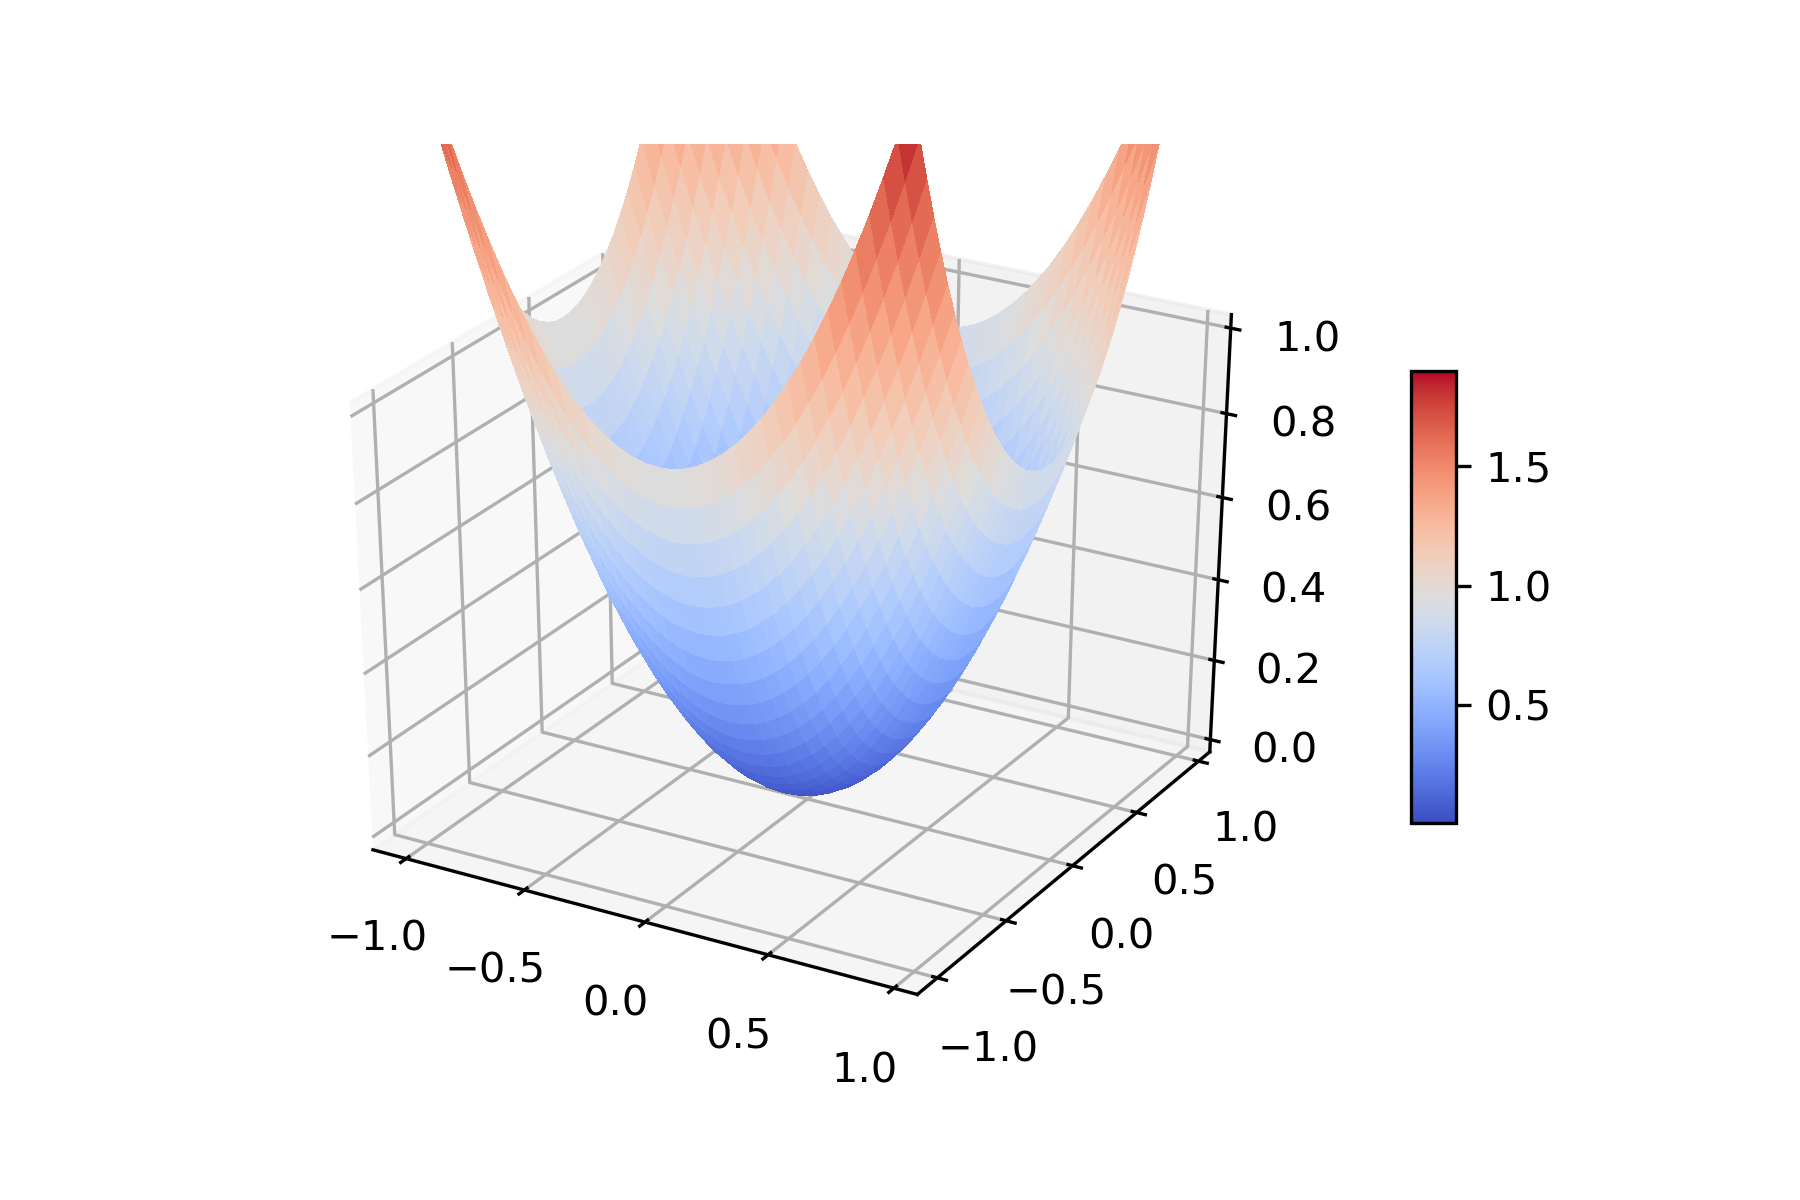
\includegraphics[scale = 0.5]{Figures/graph_positive.png}

\item Отрицательно определенная форма $z = - x^2 - y^2$.
Начало координат -- точка максимума.

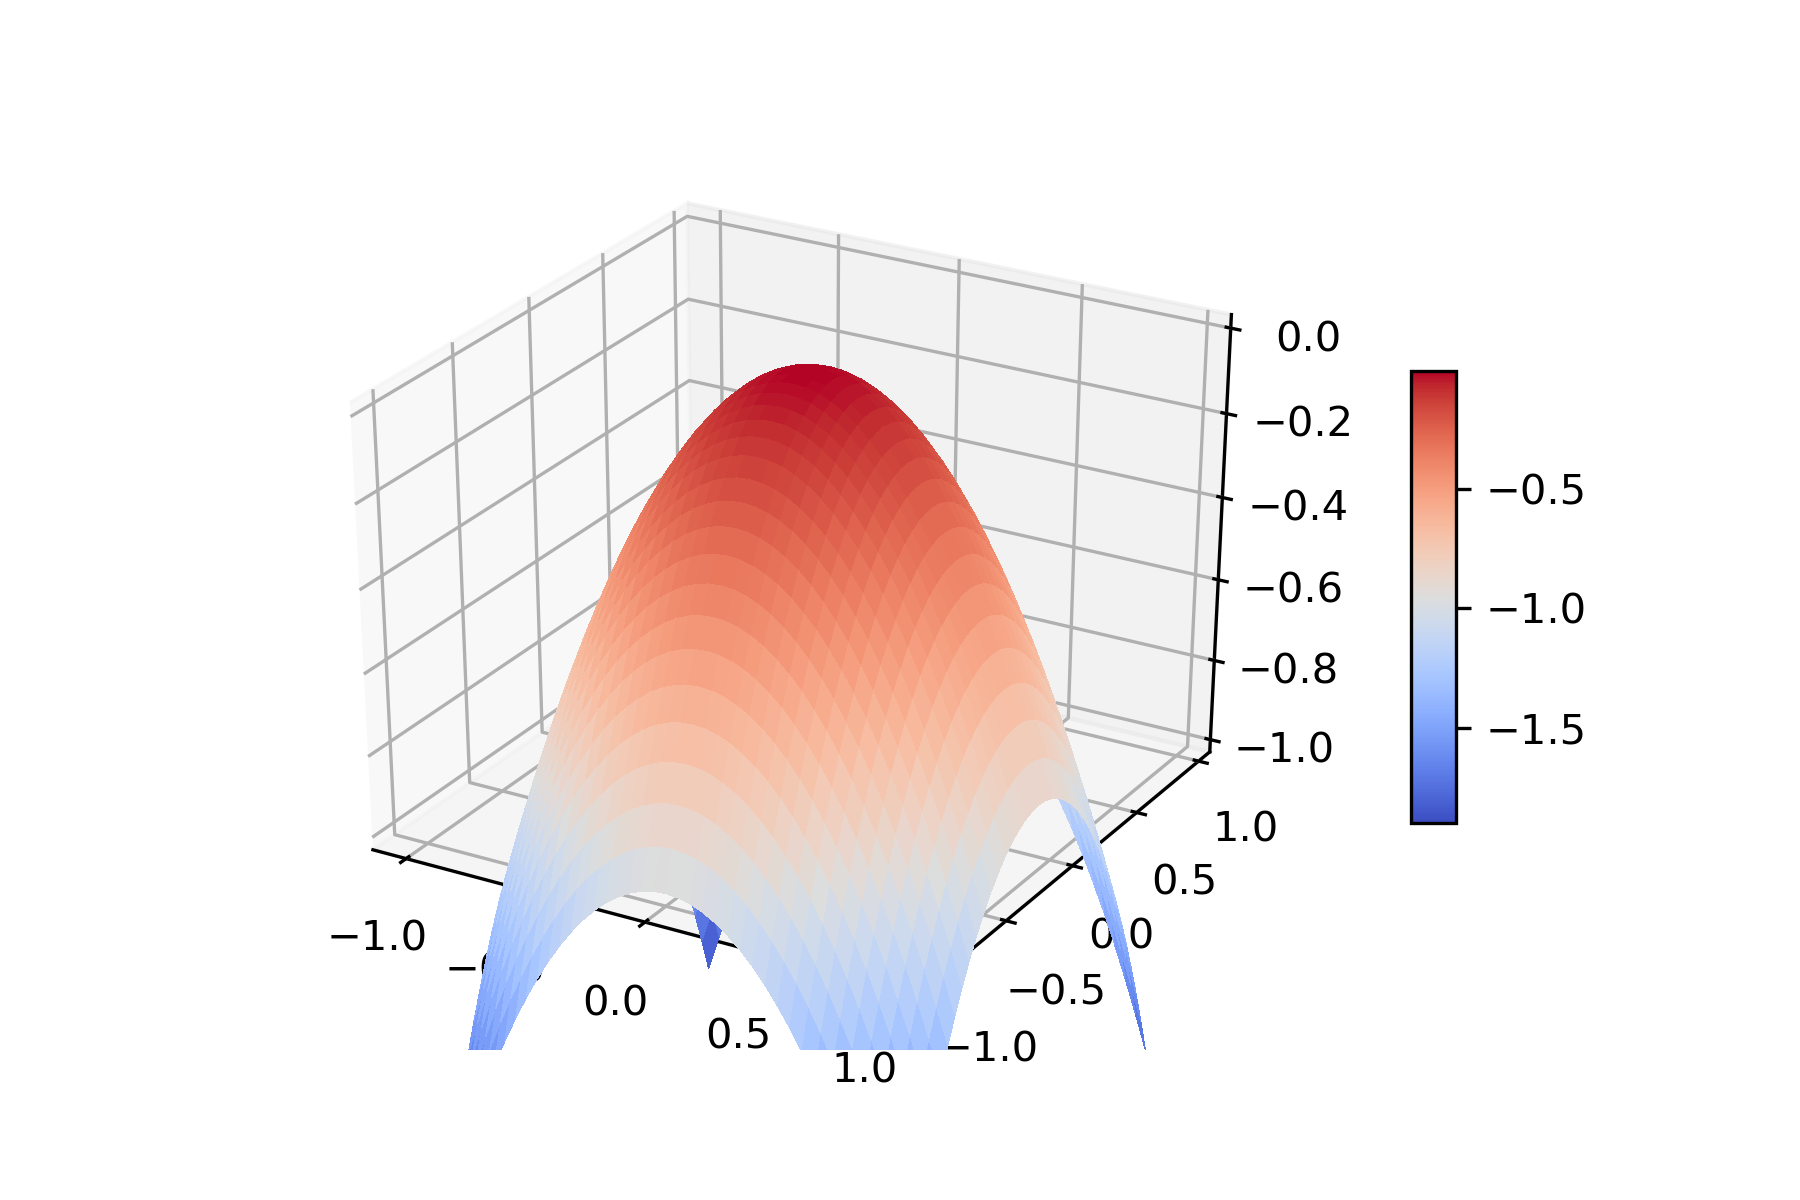
\includegraphics[scale = 0.5]{Figures/graph_negative.png}

\item Неотрицательно определенная форма $z = x^2$.
Минимум достигается на прямой $ x = 0$.

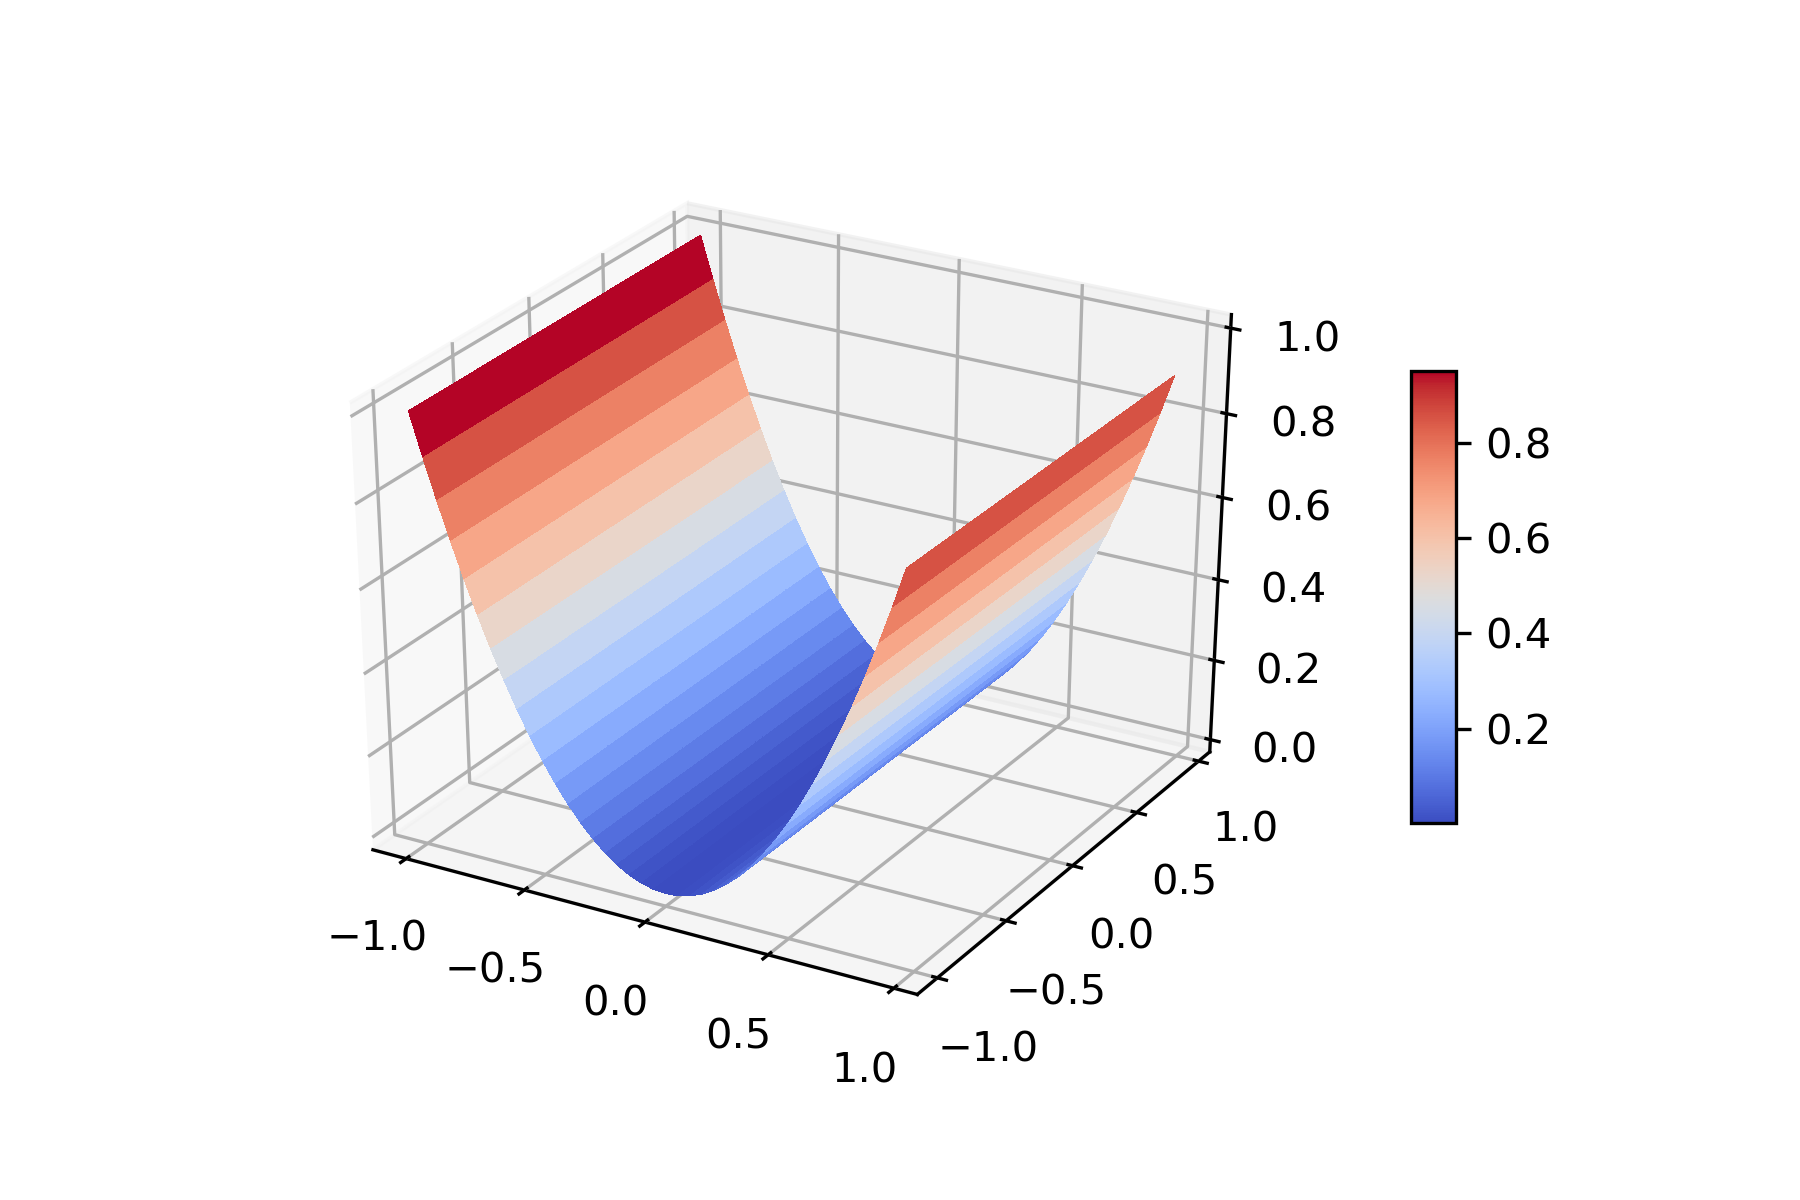
\includegraphics[scale = 0.5]{Figures/graph_non_negative.png}

\item Неположительно определенная форма $z = - x^2$.
Максимум достигается на прямой $x = 0$.

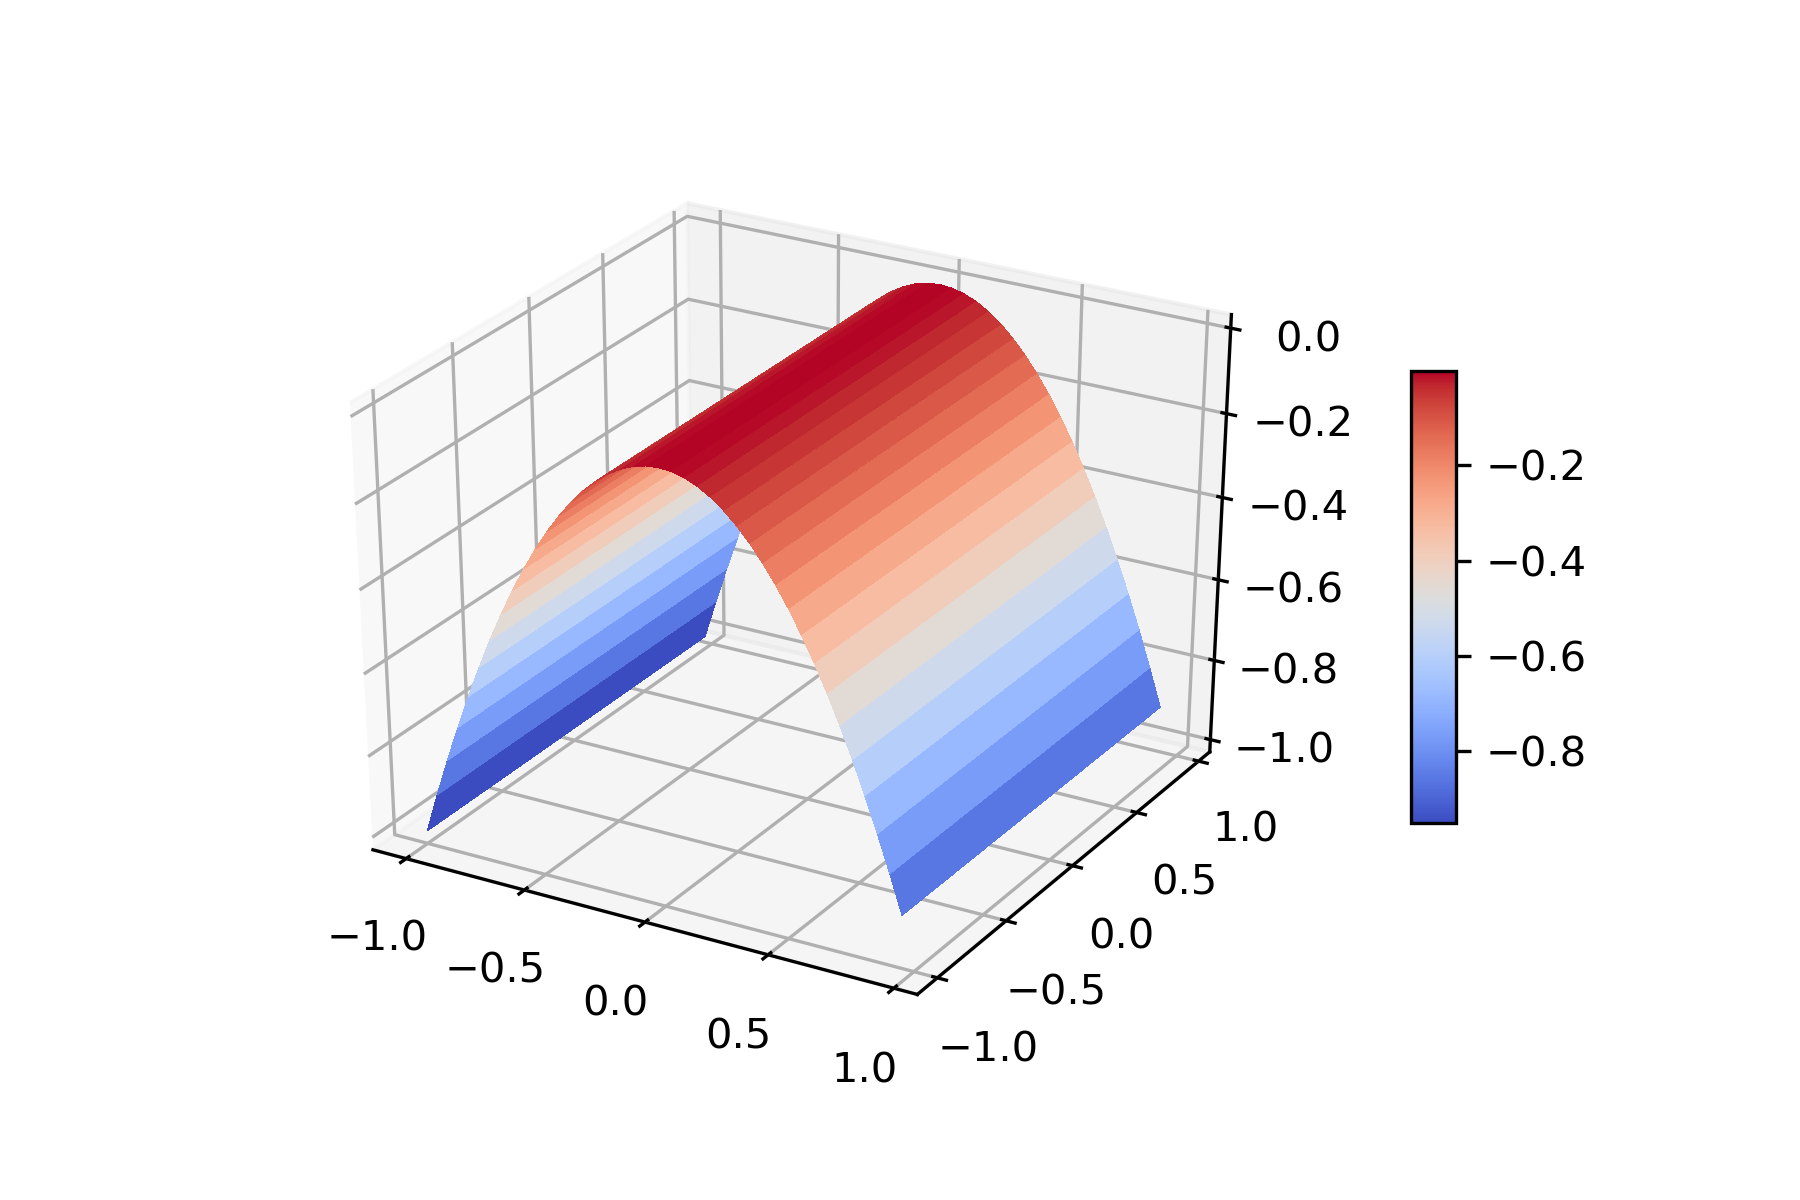
\includegraphics[scale = 0.5]{Figures/graph_non_positive.png}

\item Неопределенная форма $z = x^2 - y^2$.
Начало координат -- седловая точка.

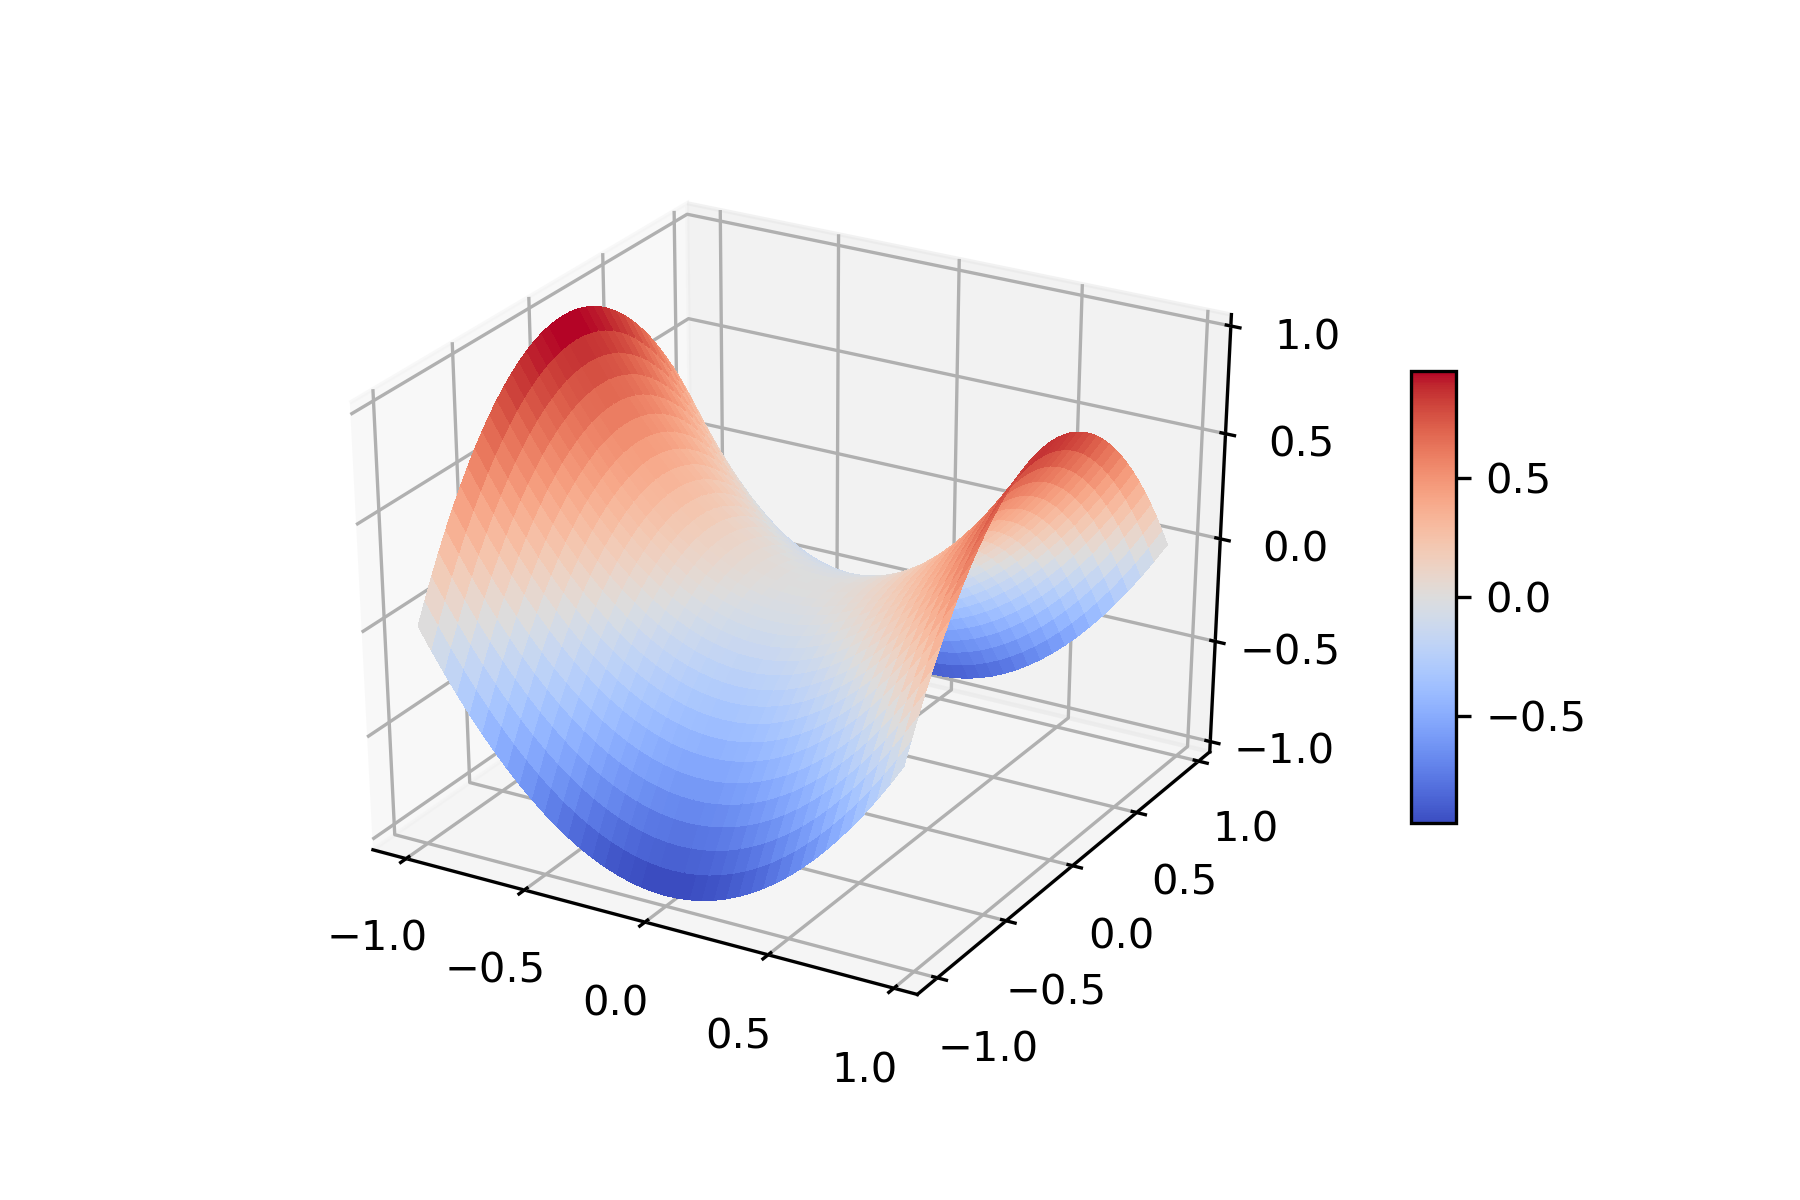
\includegraphics[scale = 0.5]{Figures/graph_saddle.png}
\end{enumerate}


\subsection{Анализ поверхности}

Квадратичные формы применяются для анализа поверхности графика функции от многих переменных.
Давайте я вкратце обрисую как.
Пусть $f\in C^2(\mathbb R^n)$ -- функция $n$ переменных, дифференцируемая дважды и вторые производные все непрерывны.
Тогда для любой точки $a\in \mathbb R^n$ выполнено разложение Тейлора
\[
f(z) = f(a) + \sum_{i=1}^n \frac{\partial f}{\partial x_i}(a)(z_i-a_i) + \sum_{ij=1}^n\frac{\partial^2 f}{\partial x_i\partial x_j}(a)(z_i-a_i)(z_j-a_j) + o(|z - a|^2)
\]
Здесь $o(|z-a|^2) = |z-a|^2 o(1)$, где $o(1)\to 0$ когда $z \to a$.
Геометрический смысл слагаемых следующий
\begin{enumerate}
\item Первое слагаемое $f(a)$ -- значение функции в точке.
Тут я никого этим не удивил.
Это лучшее приближение константой для нашей функции в точке $a$.

\item Второе слагаемое
\[
\sum_{i=1}^n \frac{\partial f}{\partial x_i}(a)(z_i-a_i)
\]
задает касательную плоскость в точке $a$ к графику функции $y = f(z)$.
То есть это линейное приближение для графика функции.
Эта плоскость горизонтальна тогда и только тогда, когда $ \frac{\partial f}{\partial x_i}(a) = 0$ для всех $1\leqslant i\leqslant n$.

\item Третье слагаемое 
\[
\sum_{ij=1}^n\frac{\partial^2 f}{\partial x_i\partial x_j}(a)(z_i-a_i)(z_j-a_j)
\]
является квадратичным приближением для графика функции.
Матрица с коэффициентами $\frac{\partial^2 f}{\partial x_i\partial x_j}(a)$ задает квадратичную форму называемую гессианом.
Если касательная плоскость горизонтальна, то сигнатура этой квадратичной формы определяет поведение графика в окрестности точки.
\begin{itemize}
\item Если форма положительно определена, то это точка локального минимума.

\item Если форма отрицательно определена, то это точка локального максимума.

\item Если форма не вырождена и неопределена, то это седловая точка
\end{itemize}
\end{enumerate}

\newpage
\section{Евклидовы пространства}

\subsection{Определение и примеры}

\begin{definition}
Евклидово пространство -- это пара $V$ и $({-},{-})$, где 
\begin{itemize}
\item $V$ -- векторное пространство над полем $\mathbb R$.

\item $({-},{-})\colon V\times V\to \mathbb R$ -- билинейная форма
\end{itemize}
При этом выполнены следующие аксиомы:
\begin{enumerate}
\item Форма $({-},{-})$ симметрическая.

\item Форма $({-},{-})$ положительно определена.
\end{enumerate}
Такая билинейная форма называется скалярным произведением.
\end{definition}

Очень часто, для краткости, когда задано евклидово пространство $V, ({-},{-})$, говорят, что $V$ является евклидовым пространством, подразумевая, что на нем есть скалярное произведение.

\paragraph{Примеры}

\begin{enumerate}
\item Пространство $\mathbb R^n$ со стандартным скалярным произведением $(x,y) = x^t y$.
Тогда $Q(x) = x^t x = \sum_{i=1}^n x_i^2 > 0$ при $x\neq 0$.

\item Пространство $\Matrix{n}$ со скалярным произведением $(A, B) = \tr(A^t B)$.
Тогда $Q(A) = \tr(A^t A) = \sum_{i,j=1}^n a_{ij}^2 > 0$ при $A\neq 0$.

\item Пусть $C[0,1]$ -- пространство непрерывных функций на отрезке $[0,1]$ сл скалярным произведением $(f,g) = \int_0^1 f(x) g(x)\,dx$.
Тогда $Q(f) = \int_0^1 f^2(x)\,dx > 0$ при $f \neq 0$.%
\footnote{В силу непрерывности, если $f(x)\neq 0$, то в какой-то окрестности $(x-\delta, x+\delta)$ точки $x$ имеем $|f(y)| > |f(x)| - \varepsilon$.}
\end{enumerate}

Важный вопрос: а как задавать скалярные произведения на некотором пространстве $V$?
Если в $V$ выбрать базис, то оно превратится в $\mathbb R^n$.
Тогда скалярное произведение задается симметричной матрицей $B$ с положительной сигнатурой.
Самый неудобный момент здесь заключается в том, что вообще говоря, глядя на матрицу $B$ не очевидно является ли она положительно определенной или нет.
Для этого надо пользоваться критерием Сильвестра (утверждение~\ref{claim::SilvCrit}).
Оказывается есть способ лучше, его мы обсудим далее.

\subsection{Ортогональные и ортонормированные базисы}

\begin{definition}
Пусть $V$ -- евклидово пространство.
Тогда
\begin{itemize}
\item Набор $v_1,\ldots,v_k\in V$ называется ортогональным, если $(v_i,v_j) = 0$ для всех $i\neq j$.

\item Набор $v_1,\ldots,v_k\in V$ называется ортонормированным, если он ортогонален и $(v_i,v_i) = 1$ для любого $i$.
\end{itemize}
Если $e_1,\ldots,e_n$ -- базис $V$, то он называется ортогональным или ортонормированным базисом, если набор $e_1,\ldots,e_n$ ортогонален или ортонормирован.
\end{definition}

\paragraph{Замечания}

\begin{itemize}
\item Базис является ортогональным тогда и только тогда, когда матрица скалярного произведения в нем диагональная.

\item Базис является ортонормированным тогда и только тогда, когда матрица скалярного произведения в нем единичная.

\item Утверждение~\ref{claim::SBilReal} говорит, что матрицу скалярного произведения всегда можно привести к единичной в некотором базисе.
То есть ортонормированные базисы существуют.

\item Процесс применяемый в методе Якоби (раздел~\ref{subsection::JacobyAlg}) превращает любой базис в ортогональный.%
\footnote{В евклидовых пространствах этот процесс называется процессом ортогонализации Грама-Шмидта.
Определение будет дальше.}
\end{itemize}

\begin{claim}
\label{claim::ScalarDef}
Пусть $V$ -- векторное пространство над $\mathbb R$.
Тогда для любого базиса $e_1,\ldots,e_n$ существует единственное скалярное произведение $({-},{-})$ на $V$ такое, что $e_1,\ldots,e_n$ является ортонормированным базисом.
\end{claim}
\begin{proof}
Зафиксируем базис $e_1,\ldots,e_n$.
Тогда задать билинейную форму -- это все равно, что задать матрицу $B\in \Matrix{n}$ (утверждение~\ref{claim::BilinearMatrices}).
Когда такая матрица $B$ задает скалярное произведение, в котором $e_1,\ldots,e_n$ -- ортонормированный базис?
Тогда и только тогда, когда $B = E$.
\end{proof}

По ортогональным и ортонормированным базисам удобно раскладывать произвольные векторы.

\begin{claim}
Пусть $V$ -- евклидово пространство, $e_1,\ldots,e_n$ -- базис и $v\in V$ -- произвольный вектор.
Тогда
\begin{enumerate}
\item Если $e_1,\ldots,e_n$ ортогональный, то 
\[
v = \frac{(v,e_1)}{(e_1,e_1)}e_1 + \ldots + \frac{(v,e_n)}{(e_n,e_n)} e_n
\]

\item Если $e_1,\ldots,e_n$ ортонормированный, то
\[
v = (v,e_1)e_1+\ldots+(v,e_n)e_n
\]
\end{enumerate}
\end{claim}
\begin{proof}
Вторая формула есть элементарное следствие первой, так как $(e_i,e_i) = 1$ для ортонормированного базиса.
Потому достаточно доказать первую формулу.
Пусть $v = \alpha_1e_1+\ldots+\alpha_n e_n$.
Умножим скалярно левую и правую часть на вектор $e_k$, тогда получим $(v, e_k) = \sum_{i=1}^n \alpha_i(e_i, e_k) = \alpha_k (e_k,e_k)$.
Значит, $\alpha_k = \frac{(v,e_k)}{(e_k,e_k)}$, что и требовалось.
\end{proof}

\begin{claim}
Пусть $A\in \Matrix{n}$.
Тогда следующие условия равносильны
\begin{enumerate}
\item $A^t A = E$.

\item $AA^t = E$.

\item $A^t = A^{-1}$.
\end{enumerate}
\end{claim}
\begin{proof}
Это следует из существования и единственности обратного при наличии левого или правого обратного (утверждение~\ref{claim::InvertibleDiscription}).
\end{proof}

\begin{definition}
Матрица $A\in \Matrix{n}$ называется ортогональной, если выполнено одно из эквивалентных свойств из предыдущего утверждения, например, $A^t A = E$.
\end{definition}

\paragraph{Замечание}

Рассмотрим в $\mathbb R^n$ стандартное скалярное произведение.
Если $A\in\Matrix{n}$, то условие $A^t A = E$ означает, что столбцы матрицы $A$ образуют ортонормированный базис.
Условие $A A^t = E$ означает, что строки матрицы $A$ образуют ортонормированный базис.
Важно понимать, что эти условия эквивалентны.
А именно, если вы возьмете ортонормированный базис в $\mathbb R^n$ и поставите эти векторы в столбцы матрицы $A$, то строки этой матрицы автоматически образуют некий другой ортонормированный базис в $\mathbb R^n$.

\begin{claim}
\label{claim::OrthoBasisDiscrEucl}
Пусть $V$ -- евклидово пространство.
Тогда
\begin{enumerate}
\item Если $e_1,\ldots,e_n$ и $f_1,\ldots,f_n$ -- два ортонормированных базиса, то матрица перехода между ними будет ортогональна.

\item Если $e_1,\ldots,e_n$ -- ортонормированный базис и $C\in \Matrix{n}$ -- ортогональная матрица, то базис $(e_1,\ldots,e_n)C$ будет ортонормированным.
\end{enumerate}
\end{claim}
\begin{proof}
(1) Пусть $(f_1,\ldots,f_n) = (e_1,\ldots,e_n)C$, где $C\in \Matrix{n}$.
Так оба базиса ортонормированные, то матрица скалярного произведения в каждом из этих базисов единичная.
По правилу изменения матрицы билинейной формы при смене базиса получаем $E = C^t E C$.
Значит $C$ ортогональная.

(2) Пусть $(f_1,\ldots,f_n) = (e_1,\ldots,e_n)C$.
В базисе $e_1,\ldots,e_n$ матрица билинейной формы $E$, так как он ортонормированный.
Матрица в базисе $f_1,\ldots,f_n$ будет $C^t E C$.
Так как $C$ ортогональная, то это будет $E$, то есть $f_1,\ldots,f_n$ -- ортонормированный базис.
\end{proof}

Таким образом за переход между ортонормированными базисами отвечают только ортогональные матрицы.

\subsection{Классификация Евклидовых пространств}

Если у нас есть два векторных пространства $V$ и $U$, то они изоморфны (то есть по сути одно и то же векторное пространство, но заданное по-разному) тогда и только тогда, когда у них одинаковые размерности (утверждение~\ref{claim::VectorClassific}).
Теперь мы хотим решить ту же самую задачу для евклидовых пространств -- понять, когда они будут одинаковыми.
Для начала надо объяснить, что значит изоморфизм евклидовых пространств.

\begin{definition}
Пусть $V$ и $U$ -- два евклидовых пространства.
Линейное отображение $\phi\colon V\to U$ называется изоморфизмом евклидовых пространств, если
\begin{enumerate}
\item $\phi$ -- изоморфизм векторных пространств.

\item Для любых $v,u\in V$ выполнено $(v, u) = (\phi(v), \phi(u))$.%
\footnote{Здесь слева скалярное произведение в пространстве $V$, а с права в пространстве $U$.}
\end{enumerate}
При наличии изоморфизма между евклидовыми пространствами $V$ и $U$ они называются изоморфными.
\end{definition}

Второе условие в определении можно выразить коммутативностью следующей диаграммы
\[
\xymatrix@R=6pt@C=40pt{
	{V\times V}\ar[dd]^{\phi\times \phi}\ar[rd]&{}&{(v,u)}\ar@{|->}[dd]\ar@{|->}[rd]&{}\\
	{}&{\mathbb R}&{}&{(v,u) = (\phi(v),\phi(u))}\\
	{U\times U}\ar[ru]&{}&{(\phi(v),\phi(u))}\ar@{|->}[ru]&{}
}
\]
Смысл определения в том, что при изоморфизме не только вектора и операции над ними переходят в соответствующие вектора и операции, но и скалярное произведение на первом пространстве превращается в скалярное произведение на втором после применения измоморфизма.
Значит при таком изоморфизме вся структура евклидова пространства сохраняется, а значит мы считаем, что такие пространства одинаковые, как евклидовы пространства.
Более того, все свойства таких пространств (если они выражены в терминах евклидова пространства) одинаковые и одно можно безболезненно менять на другое, если это удобно.

\begin{claim}
\label{claim::EuclideanIsom}
Два евклидовых пространства $V$ и $U$ изоморфны тогда и только тогда, когда $\dim V = \dim U$.
\end{claim}
\begin{proof}
Ясно, что у изоморфных пространств одинаковая размерность.
Потому надо показать, что из условия $\dim V = \dim U$ найдется изоморфизм, согласованный со скалярным произведением.
Давайте выберем ортонормированный базис $e_1,\ldots,e_n$ в $V$ и ортонормированный базис $f_1,\ldots,f_n$ в $U$.
Тогда построим линейное отображение $\phi\colon V\to U$ отправляющее $e_i\mapsto f_i$ (такое найдется единственное по утверждению~\ref{claim::LinMapExist}).
Если векторы $v,u\in V$ имеют координаты $x,y\in \mathbb R^n$ в базисе $e_1,\ldots,e_n$, то векторы $\phi(v),\phi(u)\in U$ имеют те же самые координаты $x,y$ в базисе $f_1,\ldots,f_n$.
Тогда $(v,u) = x^ty$ и $(\phi(v),\phi(u)) = x^ty$.
\end{proof}

\paragraph{Замечания}

\begin{itemize}
\item Таким образом добавление скалярного произведения к пространству не увеличивает количество не изоморфных векторных пространств.

\item Пространство $\mathbb R^2$ со стандартным скалярным произведением является <<школьной плоскостью>>, которую мы все долго и упорно изучали в курсе геометрии школьной программы.
А пространство $\mathbb R^3$ со стандартным произведением является <<школьным пространством>>.

\item Самым важным с идейной точки зрения является следующее наблюдение, которое вытекает из предыдущего утверждения.
Пусть мы хотим доказать что-то про два вектора $v,u\in V$ в каком-то евклидовом пространстве.
Тогда они обязательно содержатся в каком-то двумерном подпространстве $U\subseteq V$.
Само $U$ тоже является евклидовым вместе с ограничением скалярного произведения с $V$.
Но у нас есть школьная плоскость, которая тоже является двумерным евклидовым пространством.
А значит, это то же самое пространство, что и $U$.
То есть нам достаточно доказать факт для произвольных двух векторов на школьной плоскости.
Получается, что автоматически можно пользоваться результатами школьной геометрии.
Аналогичная идея работает с тремя векторами и сведением задачи к школьной стереометрии.

\item Несмотря на то, что можно пользоваться школьной геометрией, бывает полезно понять, как именно доказывать те или иные утверждения пользуясь формализмами линейной алгебры напрямую.
Потому я буду периодически демонстрировать какие-то вещи в лоб.
\end{itemize}

\subsection{Геометрия в Евклидовых пространствах}

\begin{definition}
Пусть $V$ -- евклидово пространство и $v\in V$ -- произвольный вектор.
Определим длину вектора $|v| = \sqrt{(v,v)}$.
\end{definition}

\paragraph{Замечания}

\begin{itemize}
\item Именно для того, чтобы определить длину произвольного вектора, нам нужна положительная определенность в определении скалярного произведения.

\item Обратите внимание, что $|v| = 0$ тогда и только тогда, когда $v = 0$.

\item Если выбрать ортонормированный базис, то $|x| = \sqrt{\sum_{i=1}^n x_i^2}$.
То есть это $|{-}|_2$ норма на $\mathbb R^n$.
На самом деле можно развивать теорию норм на произвольных векторных пространствах, как это делается в функциональном анализе.
\end{itemize}

\begin{claim}
[Неравенство Коши-Буняковского]
Пусть $V$ -- евклидово пространство, $v,u\in V$, тогда $|(v,u)|\leqslant |v| |u|$.
Кроме того, равенство достигается тогда и только тогда, когда $u$ и $v$ лежат на одной прямой.
\end{claim}
\begin{proof}
Так как у нас всего два вектора, можно считать, что $V$ двумерно.
Выберем первый базисный вектор $e_1$ вдоль $v$ (если $v$ нулевой, то выбираем любой), а второй -- любой ортогональный к $e_2$ и длины $1$.
Тогда
\[
v = 
\begin{pmatrix}
{a}\\{0}
\end{pmatrix}
\quad\text{и}\quad
u = 
\begin{pmatrix}
{b}\\{c}
\end{pmatrix}
\]
Тогда $|(v, u)| = |ab|$, а $|v||u| = |a|\sqrt{b^2 + c^2}$.
Доказываемое неравенство превращается в $|ab|\leqslant |a|\sqrt{b^2 + c^2}$, что очевидно.

Давайте проанализируем, когда в нем достигается равенство.
Во-первых, если $a = 0$.
В этом случае $v$ и $u$ лежат на одной прямой.
Если $a \neq 0$, то мы получаем условие $|b| = \sqrt{b^2 + c^2}$, что равносильно тому, что $c = 0$.
В этом случае векторы тоже лежат на одной прямой.
Обратно, если векторы лежат на одной прямой, то $v = \lambda e$ и $u = \mu e$ для некоторого ненулевого вектора $e\in V$.
Тогда $(v,u) = \lambda\mu (e,e)$, а с другой стороны $|v||u| = |\lambda e||\mu e| = |\lambda \mu| |e|^2 = |\lambda \mu|(e,e)$.
\end{proof}

\paragraph{Замечание} 

Хочу обратить внимание на то, что по сути доказательство можно было закончить на первой строчке, где я ссылаюсь  на школьную геометрию.
Вся остальная часть всего лишь доказывала факт из школьной геометрии.
Это было сделано для полноты изложения.
К тому же я продемонстрировал метод последовательного выбора удобных базисных векторов, который часто применяется при решении задач аналитической геометрии.
Подобный метод позволяет упростить разбор общего случая в координатах за счет наличия большого количества нулей в векторах.
В нашем случае ноль был всего один, но это сильно сократило вычисления.

Из неравенства Коши-Буняковского следует, что для любых двух ненулевых векторов $v,u\in V$ верно $-1\leqslant \frac{(v,u)}{|v| |u|}\leqslant 1$.
А значит найдется единственное число $\alpha\in [0,\pi]$ такое, что $\cos \alpha = \frac{(v,u)}{|v| |u|}$.

\begin{definition}
Пусть $V$ -- евклидово пространство и $v,u\in V$ -- два вектора.
Тогда число $\alpha$ такое, что $\cos \alpha = \frac{(v,u)}{|v| |u|}$, называется углом между векторами $v$ и $u$.
Будем этот угол обозначать через $\angle(v, u)$.
\end{definition}

\paragraph{Замечание}

Так как два вектора $v$ и $u$ всегда лежат внутри <<школьной плоскости>>, то определение угла превращается в то самое определение угла, которое дается в школьном курсе геометрии.
Потому от этого угла надо ожидать ровно то же самое поведение, к которому мы привыкли в курсе школьной геометрии.
Просто потому, что это тот же самый угол.

\begin{claim}
[Теорема Пифагора]
\label{claim::Pythagoras}
Пусть $V$ -- евклидово пространство и $v,u\in V$ -- два ортогональных вектора, тогда $|v + u|^2 = |v|^2 + |u|^2$.
\end{claim}
\begin{proof}
Формальное доказательство в этом случае является наиболее простым:
\[
|v+u|^2 = (v+u, v+u) = (v,v) + (v,u)+(u,v) +(u,u) = (v,v) + (u,u) = |v|^2 + |u|^2
\]
Здесь $(v,u)=(u,v) = 0$ из ортогональности $u$ и $v$.
\end{proof}

Процесс, применяемый к базисным векторам в методе Якоби (раздел~\ref{subsection::JacobyAlg}), в случае евклидова пространства называется ортогонализацией Грама-Шмидта.
Единственное отличие -- ортогонализация Грама-Шмидта применяется не только к линейно независимым векторам, а к произвольным системам векторов.

\subsubsection*{Ортогонализация методом Грама-Шмидта}

\paragraph{Дано}

Евклидово пространство $V$, система векторов $\{v_1,\ldots,v_k\}\subseteq V$.%
\footnote{Обратите внимание, что $V$ не обязательно задано как пространство столбцов $\Vector{n}$.
Это может быть и пространство многочленов определенной степени или пространство тригонометрических функций, или вообще что угодно.
Даже если $V$ задано как $\Vector{n}$, то скалярное произведение не обязательно стандартное, т.е. скалярное произведение может быть задано любой положительной симметрической матрицей.}

\paragraph{Задача}

Найти систему ортогональных векторов $\{u_1,\ldots,u_r\}\subseteq V$ такую, что $\langle v_1,\ldots,v_k\rangle = \langle u_1,\ldots,u_r\rangle$.

\paragraph{Алгоритм}

\begin{enumerate}
\item В качестве первого вектора $u_1$ берем первый ненулевой вектор из $v_i$.
Если таких нет, то ответ -- пустое множество.

\item Пусть мы нашли вектора $u_1,\ldots,u_s$ и пусть $v_d$ -- первый еще не просмотренный вектор среди $v_i$.
Посчитать вектор 
\[
u' = v_d - \frac{(v_d, u_1)}{(u_1,u_1)} u_1 - \ldots - \frac{(v_d, u_s)}{(u_s, u_s)}u_s
\]

\item Если $u' \neq 0$ положим $u_{s+1} = u'$, иначе пропустим $v_d$.
Теперь перейдем к предыдущему шагу с вектором $v_{d+1}$ вместо $v_d$.
\end{enumerate}

\ProvidesFile{lecture29.tex}[Лекция 29]


\subsection{Проекции}
\label{section::OrthoProjection}

\begin{claim}
Пусть $V$ -- евклидово пространство и $U\subseteq V$ -- произвольное подпространство.
Тогда $V = U\oplus U^\bot$.
\end{claim}
\begin{proof}
Это в точности утверждение~\ref{claim::NonDegRestrictionBil} пункт~(2).
\end{proof}

Таким образом в евклидовом пространстве $V$ при фиксированном подпространстве $U\subseteq V$, любой вектор $v\in V$ единственным образом раскладывается в сумму $v = \pr_U v + \ort_U v$, где $\pr_U v \in U$ и $\ort_U v\in U^\bot$.

\begin{definition}
Если $V$ -- евклидово пространство, $U\subseteq V$ -- произвольное подпространство и $v\in V$, то 
\begin{itemize}
\item Вектор $\pr_U v$ называется ортогональной проекцией $v$ на $U$.

\item Вектор $\ort_U v$ называется ортогональной составляющей $v$ относительно $U$.
\end{itemize}
\end{definition}

Обратите внимание, что ортогональная проекция $v$ на $U$ -- это проекция $v$ на $U$ вдоль $U^\bot$, а ортогональная составляющая -- проекция $v$ на $U^\bot$ вдоль $U$.

\subsubsection*{Формула БАБА}

Давайте я в начале разберу задачу нахождения проекции вектора на подпространство вдоль другого подпространства (здесь нам не нужно никакое скалярное произведение).
Пусть $V$ -- некоторое векторное пространство и $V = U\oplus W$.
Тогда на пространстве $V$ задан оператор проекции $P\colon V\to V$ такой, что $\ker P = W$ и $P|_U = \Identity$, то есть, если $v\in V$ раскладывается в сумму $v = u + w$, где $u\in U$ и $w\in W$, то $Pv = u$ -- оператор вычисления проекции на $U$ вдоль $W$.


Теперь мы хотим научиться эффективно считать $P$.
Для этого предположим $V = \mathbb R^n$, $U = \langle u_1,\ldots,u_k\rangle$, $W = \{y\in \mathbb R^n\mid Ay = 0\}$, где $A\in \MatrixDim{s}{n}$.
В этом случае $P\colon \mathbb R^n\to \mathbb R^n$ задается некоторой матрицей.
Наша задача -- найти эту матрицу.

Предположим для простоты, что векторы $u_1,\ldots,u_k$ образуют базис $U$, а строки матрицы $A$ линейно независимы.
Определим матрицу $B = (u_1|\ldots|u_k)\in \MatrixDim{n}{k}$.
Тогда утверждаются следующие вещи:
\begin{enumerate}
\item Количество столбцов $B$ совпадает с количеством строк $A$, то есть $k = s$.

\item Матрица $AB$ обратима.

\item Оператор проекции задается формулой $P = B(AB)^{-1}A$.
Мнемоническое правило <<БАБА>>.
\end{enumerate}
\begin{proof}
Так как мы уже взрослые, я позволю себе пользоваться линейными операторами и отображениями, а не просто матричной техникой.
Матрица $A$ задает линейное отображение $A\colon \mathbb R^n \to \mathbb R^s$ такое, что $\ker A = W$ и $\Im A = \mathbb R^s$ (так как строки матрицы $A$ линейно независимы, то $\rk A = s$, но $\rk A = \dim \Im A$).
Матрица $B$ задает отображение $B\colon \mathbb R^k \to \mathbb R^n$ такое, что $\Im B = U$ и $\ker B = 0$ (так как столбцы $B$ линейно независимы).

(1) Теперь мы знаем, что 
\[
\begin{aligned}
\dim U + \dim W = n\\
\dim \ker A + \dim \Im A = n
\end{aligned}
\quad\text{ то есть }\quad
\begin{aligned}
k + \dim W = n\\
\dim W+ s= n
\end{aligned}
\quad\text{ откуда }\quad
s = k
\]

(2) Теперь рассмотрим отображение $AB\colon \mathbb R^k \to \mathbb R^k$.
Заметим, что $\Im B \cap \ker A = U \cap W = 0$.
Значит $\ker AB = 0$, то есть $AB$ -- обратимый оператор.

(3) Теперь выведем формулу для $P$.
Пусть $v = u + w$, где $v\in \mathbb R^n$ -- произвольный вектор, $u\in U$ и $w\in W$ -- его единственное разложение по прямой сумме подпространств.
Тогда $Av = Au + Aw = Au$.
С другой стороны, так как $u\in U$, мы имеем $u = B x$ для некоторого $x\in \mathbb R^k$.
Тогда $Av = ABx$.
Так как $AB$ обратимая квадратная матрица, имеем $x = (AB)^{-1}Av$.
Значит $u = Bx = B(AB)^{-1}Av$, что и требовалось.
\end{proof}

Обратите внимание, что проектор $P$ на $U$ вдоль $W$ зависит от двух подпространств, а не только от $U$.
Если вы измените одно из них, то проектор изменится.

\subsubsection*{Формула Атата}

Пусть $V = \mathbb R^n$ со стандартным скалярным произведением $(x, y) = x^ty$ и пусть подпространство $U\subseteq V$ задано своим базисом $U = \langle u_1,\ldots,u_k\rangle$.
Составим матрицу $A = (u_1|\ldots|u_k)\in\MatrixDim{n}{k}$.
Тогда $U^\bot = \{y\in \mathbb R^n \mid A^t y = 0\}$.
Пусть теперь $v\in V$ -- произвольный вектор и $v = \pr_U v + \ort_U v$.
Тогда формула <<БАБА>> превращается в $\pr_U v = A(A^tA)^{-1}A^tv$.
Мнемоническое правило для запоминания: в евклидовом пространстве БАБА -- это Атата.

Обратите внимание, что проектор $P$ всегда зависит от двух подпространств: то, на которое проектируем $U$, и то, вдоль которого проектируем $W$.
Но в случае ортогонального проектирования $W = U^\bot$, потому ортопроектор $P$ реально зависит только от одного подпространства.

\subsection{Расстояния и углы}

\begin{definition}
Пусть $V$ -- евклидово пространство и $u,v\in V$ -- произвольные векторы.
Тогда определим расстояние между векторами по формуле $\rho(u,v) = |u - v|$.
\end{definition}

\begin{claim}
Расстояние $\rho$ на евклидовом пространстве $V$ удовлетворяет следующим свойствам:
\begin{enumerate}
\item {\bf Невырожденность} $\rho(v,u) \geqslant 0$ для любых $u,v\in V$ причем равенство достигается тогда и только тогда, когда $v = u$.

\item {\bf Симметричность} $\rho(u,v) = \rho(v,u)$ для любых $u,v\in V$.

\item {\bf Неравенство треугольника} $\rho(u,v)\leqslant \rho(u,w) + \rho(w,v)$ для любых $u,v,w\in V$.
\end{enumerate}
\end{claim}
\begin{proof}
(1) По определению $\rho(v,u) = |v-u| \geqslant 0$ причем равенство достигается тогда и только тогда, когда $v - u = 0$.

(2) По определению $\rho(v, u) = |v - u| = |u-v| = \rho(u,v)$.

(3) Нам надо доказать $\rho(u,v)\leqslant \rho(u,w) + \rho(w,v)$, то есть $|u-v|\leqslant |u-w| + |w - v|$.
Положим $x = u - w$ и $y = w - v$.
Тогда нам надо доказать $|x + y|\leqslant |x| + |y|$.
Так как левая и правая части этого неравенства неотрицательные, то оно равносильно неравенству $|x+y|^2\leqslant (|x| + |y|)^2$.
Проверяем:
\[
|x+y|^2 = (x+y, x+y) = (x, x) + 2(x, y) + (y,y) = |x|^2 + 2 (x, y) + |y|^2
\]
По неравенству Коши-Буняковского $(x, y)\leqslant |x| |y|$.
Значит
\[
|x|^2 + 2 (x, y) + |y|^2\leqslant |x|^2 + 2|x||y| + |y|^2= (|x|+|y|)^2
\]
\end{proof}

\paragraph{Замечание}

Если на множестве $X$ задана функция $\rho\colon X\times X\to \mathbb R$ со свойствами из предыдущего утверждения, то пара $(X,\rho)$ называется метрическим пространством.
Самое главное, что известно про метрические пространства -- принцип сжимающих отображений.
Это один из способов доказывать существование объектов с  нужными свойствами.
Есть два важных примера:
\begin{itemize}
\item Теорема о неявной функции.
Ее доказательство через принцип сжимающих отображений в разы проще и доступнее, чем копание в координатах.

\item Теорема о существовании и единственности решения дифференциального уравнения.
Дифференциальное уравнение обычно заменяется на интегральное, после чего можно пользоваться метрическими пространствами и принципом сжимающих отображений.
\end{itemize}
В нашем случае метрика на евклидовом пространстве скорее является случайным гостем, заглянувшем на огонек, нежели чем-то фундаментальным и сверх полезным.
Самым полезным является понимание роли метрических пространств.

\begin{definition}
Пусть $X,Y\subseteq V$ -- произвольные подмножества евклидова пространства, тогда расстояние между ними определяется следующим образом:
\[
\rho(X, Y) = \inf_{\substack{x\in X\\y\in Y}}\rho(x, y)
\]
\end{definition}
Обратите внимание, что это расстояние не удовлетворяет аксиоме не вырожденности, то есть расстояние между разными множествами может быть нулевым.
Например, для этого достаточно, чтобы $X$ и $Y$ имели непустое пересечение.
Но, даже если $X\cap Y = \varnothing$, расстояние может быть нулем.
Например, если $X, Y \subseteq \mathbb R$ и $X = \{\frac{1}{n}\mid n\in \mathbb N\}$ и $Y = - X = \{-\frac{1}{n}\mid n\in \mathbb N\}$.

\begin{definition}
Пусть $V$ -- евклидово пространство, $v\in V$ и $L\subseteq V$ -- некоторое подпространство.
Тогда углом между $v$ и $L$ называется $\angle (v, L) = \inf_{u\in L}\angle (v,u)$.
\end{definition}

Теперь давайте обсудим, как эффективно находить некоторые расстояния и углы.

\begin{claim}
\label{claim::DistAngle}
Пусть $V$ -- евклидово пространство, $L\subseteq V$ -- подпространство, $v\in V$ -- некоторый вектор.
Тогда
\begin{enumerate}
\item $\rho(v, L) = |\ort_L v|$.

\item $\angle(v, L) = \angle(v, \pr_L v)$.%
\footnote{Если $\pr_L v = 0$, то надо считать косинус угла нулевым, то есть угол равным $\pi/2$.}
\end{enumerate}
\end{claim}
\begin{proof}
(1) Пусть $u\in L$ -- произвольный вектор отличный от $\pr_L v$.
Достаточно показать, что 
\[
\rho(v, u) > \rho (v, \pr_Lv) = |v - \pr_Lv| = |\ort_L v|
\]
Рассмотрим треугольник образованный концами следующих трех векторов: $v$, $\pr_Lv$, $u$.
Сторона $v - \pr_Lv = \ort_L v$ ортогональна стороне $u - \pr_L v \in L$.
Значит $u - v$ -- гипотенуза прямоугольного треугольника.Тогда по теорема Пифагора (утверждение~\ref{claim::Pythagoras})
\[
\rho(v,u) = |u - v| = \sqrt{|\ort_Lv|^2 + |u - \pr_Lv|^2 }> |\ort_Lv|
\]
Последнее неравенство строгое, так как $u\neq \pr_Lv$.

(2) В начале рассмотрим случай $\pr_L v = 0$.
Это значит, что вектор $v$ ортогонален $L$ и угол с любым вектором $\pi/2$.
Теперь предположим, что $\pr_L v \neq 0$.
Выберем произвольный вектор $u\in L$ отличный от $\pr_L v$ и имеющий такую же длину, как $\pr_L v$.
Тогда рассмотрим два треугольника: первый на векторах $0$, $v$, $\pr_Lv$, второй $0$, $v$, $u$.
Тогда у обоих треугольников стороны при вершине $0$ попарно одинаковой длины, а противоположные стороны -- $\ort_L v$ и $u - v$ соответственно.
Но по доказанному выше $|\ort_L v| < |u - v|$.
А школьная геометрия учит нас, что в этом случае угол в первом треугольнике меньше, чем во втором.

\paragraph{формальное доказательство}

Для любителей формализма я приготовил второе доказательство.
Случай $\pr_L v = 0$ разбирается так же как и выше.
Случай $\ort_L v = 0$ означает, что $v\in L$.
В этом случае угол между вектором и пространством нулевой и минимум достигается на $u = v$.
Теперь считаем, что $\pr_L v \neq 0$, $\ort_L v \neq 0$ и выберем произвольный вектор $u\in L$ такой, что $|u| = |\pr_L v|$.
Теперь выберем единичный вектор $e_1$ пропорциональный $\pr_L v$.
Выберем единичный вектор $e_2$ в плоскости $\langle \pr_Lv, u\rangle$ ортогональным $e_1$.
Единичный вектор $e_3$ выберем  пропорциональным $\ort_L v$.
Тогда все интересные нам векторы живут в пространстве $\langle e_1,e_2,e_3\rangle$.
Давайте запишем их в этом базисе
\[
v = 
\begin{pmatrix}
{\lambda}\\{0}\\{\mu}
\end{pmatrix},\quad
\pr_Lv = 
\begin{pmatrix}
{\lambda}\\{0}\\{0}
\end{pmatrix},\quad
u = 
\begin{pmatrix}
{a}\\{b}\\{0}
\end{pmatrix},\quad
\text{причем}\quad
\lambda^2 = a^2 + b^2,\;\lambda > 0
\]
Условие $v = \pr_Lv$ означает $b = 0$ и $\lambda = a$.
Нам надо показать, что $\angle (v, \pr_L v) < \angle (v, u)$.
То есть $\cos \angle (v, \pr_L v) > \cos \angle (v, u)$.
То есть надо показать, что 
\[
\frac{(v, \pr_L v)}{|v||\pr_L v|} > \frac{(v, u)}{|v||u|}
\]
Но так как $|u| = |\pr_Lv|$ по выбору, нам надо доказать, что $(v, \pr_L v) > (v, u)$, то есть, что $\lambda^2 > \lambda a$.
Из условия $\lambda^2 = a^2 + b^2$ видно, что $|\lambda| > |a|$ при $b \neq 0$.
Значит $\lambda^2 > |\lambda a|$ при $b \neq 0$.
При $b = 0$ имеем $a = \lambda$ либо $a = -\lambda$.
Если $u \neq \pr_L v$, то возможно только $a = -\lambda$, но тогда неравенство очевидно.
\end{proof}

\paragraph{Замечания}

\begin{itemize}
\item Обратите внимание, что угол между вектором и подпространством всегда находится в интервале $[0, \pi/2]$ или что то же самое косинус угла всегда неотрицательный.

\item Заметим следующую связь $\angle (v, \pr_L v) + \angle (v, \ort_L v) = \pi/2$.
Причем формула верна даже когда проекция или ортогональная составляющая равны нулю.
В этом случае соответствующий угол надо считать равным $\pi/2$.

\item Предположим, что подпространство $L\subseteq V$ имеет коразмерность $1$, то есть $\dim L = \dim V - 1$.
Тогда у нас $L^\bot$ -- одномерно.
Пусть $n\in L^\bot$ какой-нибудь ненулевой вектор.
Таким образом $n$ -- вектор нормали к $L$.
В этом случае $n$ лежит с $\ort_L v$ на одной прямой (может быть сонаправлен ему или смотреть в противоположную сторону).
Тогда $\angle (v, \ort_L v)$ равен либо $\angle (v, n)$ либо $\angle (v, - n)$ (на самом деле не большему из этих двух).
То есть в этом случае можно взять к $L$ произвольную нормаль $n$, посчитать угол $\alpha$.
Если он оказался больше $\pi/2$ заменить его на $\pi - \alpha$.
После чего найти угол с подпространством как $\pi/2$ минус полученный угол.
\end{itemize}


\subsection{Метод наименьших квадратов}

Пусть мы хотим решить систему $Ax = b$, где $A\in \MatrixDim{m}{n}$, $b\in \mathbb R^m$ и $x\in \mathbb R^n$ -- столбец неизвестных.
И предположим, что система не имеет решений, но от этого наше желание ее решить не становится слабее.
Давайте обсудим, как удовлетворить наши желания в подобной ситуации и когда такие ситуации обычно встречаются.

Введем на пространстве $\mathbb R^m$ стандартное скалярное произведение $(x,y) = x^t y$.
Тогда, на процесс решения системы можно смотреть так: мы подбираем $x\in \mathbb R^n$ так, чтоб $\rho(Ax, b) = 0$.
Если решить систему невозможно, то этот подход подсказывает, как надо поступить.
Надо пытаться минимизировать расстояние между $Ax$ и $b$.
То есть решить задачу
\[
\begin{aligned}
&\rho(Ax, b)\to \min\\
&x\in \mathbb R^n
\end{aligned}
\]
Теперь давайте поймем, как надо решать такую задачу.
Пусть матрица $A$ имеет вид $A = (A_1|\ldots|A_n)$, где $A_i\in \mathbb R^m$ -- ее столбцы.
Тогда система $Ax = b$ означает, $x_1A_1 + \ldots + x_n A_n = b$.
То есть система разрешима тогда и только тогда, когда $b\in \langle A_1,\ldots, A_n\rangle$.
Значит наша задача минимизировать расстояние между $b$ и $\langle A_1,\ldots,A_n\rangle$.
Тогда утверждение~\ref{claim::DistAngle} подсказывает, что минимум расстояния достигается на $b_0 = \pr_{\langle A\rangle}b$.
В этом случае вместо исходной системы $Ax = b$ мы должны решить систему $Ax = b_0$.
И если $x_0$ -- ее решение, то $\rho(Ax_0, b)$ как раз и будет минимальным.

Давайте теперь предположим, что столбцы матрицы $A$ линейно независимы.
Тогда по формуле <<Атата>> мы знаем, что $b_0 = A(A^tA)^{-1}A^tb$.
Кроме этого должно выполняться $b_0 = Ax_0$.
Так как столбцы $A$ линейно независимы, такое $x_0$ должно быть единственным.
Но мы видим, что в качестве $x_0$ подходит $x_0 = (A^tA)^{-1}A^tb$.

\subsection{Матрица Грама}
\label{subsection::Gram}

Давайте поговорим о еще одном объекте, который возникает в связи с конечной системой векторов в Евклидовом пространстве.
Таким объектом является матрица Грама.
Она в частности используется для определения объемов.

\begin{definition}
Пусть $V$ -- евклидово пространство и $v_1,\ldots,v_k\in V$ -- произвольный набор векторов ($k$ НЕ обязательно равно размерности пространства).
Тогда матрица
\[
G(v_1,\ldots,v_k) =
\begin{pmatrix}
{(v_1,v_1)}&{\ldots}&{(v_1,v_k)}\\
{\vdots}&{\ddots}&{\vdots}\\
{(v_k,v_1)}&{\ldots}&{(v_k,v_k)}\\
\end{pmatrix}
\in\Matrix{k}
\]
называется матрицей Грама системы векторов $v_1,\ldots,v_k$.%
\footnote{Обратите внимание, тут важен порядок векторов.
То есть формально матрица Грама зависит от набора $(v_1,\ldots,v_k)\in V^k$.}
\end{definition}

Если $e_1,\ldots,e_n$ -- некоторый базис пространства $V$, то $B = G(e_1,\ldots,e_n)$ -- матрица скалярного произведения заданная в базисе $e_1,\ldots,e_n$.
Таким образом матрица Грама -- это некоторое обобщение матрицы билинейной формы.

Теперь вспомним, что у любой билинейной формы есть операторная запись.
Давайте введем следующее обозначение: для произвольных векторов $w, u\in V$ положим $w\cdot u = (w, u)$.
Тогда для набора $v = (v_1,\ldots,v_k)$ выполнено
\[
G(v_1,\ldots,v_k) = 
\begin{pmatrix}
{v_1}\\{\vdots}\\{v_k}
\end{pmatrix}
\cdot
\begin{pmatrix}
{v_1}&{\ldots}&{v_k}
\end{pmatrix}
=
v^t \cdot v
\]

Пусть теперь $C\in \MatrixDim{k}{r}$ -- некоторая матрица.
Тогда из набора $(v_1,\ldots,v_k)$ можно построить новый набор $(u_1,\ldots,u_r) = (v_1,\ldots,v_k)C$ или кратко $u = vC$.
Тогда 
\[
G(u) = G(vC) = (vC)^t \cdot vC = C^t v^t \cdot v C = C^t G(v) C
\]
То есть $G((v_1,\ldots,v_k)C) = C^t G(v_1,\ldots,v_k)C$.

\begin{claim}
\label{claim::GramMatrixFull}
Пусть $v_1,\ldots,v_k\in V$ -- произвольный набор векторов в евклидовом пространстве.
Тогда
\begin{enumerate}
\item Пусть $\alpha_1,\ldots,\alpha_k \in \mathbb R$, введем обозначение $\alpha = (\alpha_1,\ldots,\alpha_k)^t$.
Тогда следующие условия эквивалентны:
\begin{enumerate}
\item $\alpha_1 v_1 + \ldots + \alpha_k v_k = 0$.

\item $G(v_1,\ldots,v_k)\alpha= 0$.

\item $\alpha^tG(v_1,\ldots,v_k)\alpha= 0$.
\end{enumerate}

\item $\rk G(v_1,\ldots,v_k) = \dim \langle v_1,\ldots,v_k\rangle$.

\item  $\det G(v_1,\ldots,v_k)\geqslant 0$.
При этом равенство достигается тогда и только тогда, когда векторы линейно зависимы.

\item Если $C\in\Matrix{k}$ является матрицей элементарного преобразования I или II типа, то 
\[
\det G(v_1,\ldots,v_k) = \det G((v_1,\ldots,v_k)C)
\]
\end{enumerate}
\end{claim}
\begin{proof}
1) Пусть $v = (v_1,\ldots,v_k)$.
Тогда условие $v\alpha = 0$ влечет, что $v^t \cdot v\alpha = 0$.
Но это означает, что $G(v_1,\ldots,v_k) \alpha = 0$.
Домножая слева на $\alpha^t$ получаем, что $\alpha^t G(v_1,\ldots,v_k) \alpha = 0$.
Осталось показать из последнего в первое.
Для этого заметим, что $0 = \alpha^t G(v_1,\ldots,v_k) \alpha = \alpha^t v^t \cdot v\alpha = (v\alpha, v\alpha)$.
А значит $v\alpha = 0$.

2) Пункт~(1) эквивалентность (a) и (b) означает, что векторы $v_1,\ldots,v_k$ обладают теми же линейными зависимостями, что и столбцы матрицы $G(v_1,\ldots,v_k)$.
В частности столбцовый ранг $G(v_1,\ldots,v_k)$ равен рангу системы векторов $(v_1,\ldots,v_k)$.
А последняя совпадает с размерностью линейной оболочки $\langle v_1,\ldots,v_k\rangle$.

3) Давайте на пространстве $\mathbb R^k$ рассмотрим билинейную форму $\beta(x,y) = x^t G(v_1,\ldots,v_k)y$.
Давайте покажем, что она не отрицательно определена.
Тогда, ее определитель должен быть не отрицательным.
Действительно, тогда в каком-то базисе ее матрица диагональна с $1$ и $0$ на диагонали, а значит в этом базисе определитель будет неотрицательным.
Но определитель билинейной формы не меняет знак при замене базиса (раздел~\ref{subsection::BilChar}).
Теперь остается лишь проверить, что $\beta(x,x)\geqslant 0$ для любого $x\in \mathbb R^k$.
Действительно
\[
x^t G(v_1,\ldots,v_k) x = x^t v^t\cdot v x = (vx, vx) \geqslant 0
\]
Последнее неравенство выполнено для любого вектора $vx\in V$ по определению скалярного произведения.

4) Если $C$ -- матрица элементарного преобразования, то $G((v_1,\ldots,v_k)C) = C^t G(v_1,\ldots,v_k)C$.
А значит $\det(G((v_1,\ldots,v_k)C)) = \det(G(v_1,\ldots,v_k))\det C^2$.
Но для элементарных преобразований I и II типов $\det C = \pm 1$.
\end{proof}

Заметим, что из третьего пункта следует вот какое наблюдение.
Если $v_1,\ldots, v_k$ -- линейно независимый набор векторов, из которого процессом ортогонализации Грама-Шмидта мы получили набор $u_1,\ldots,u_k$, то $\det G(u_1,\ldots,u_k) = \det G(v_1,\ldots,v_k)$.

\subsection{Объемы}

Теперь самое время прикоснуться к объемам.
Надо сказать, что существует общая теория вычисления объемов в евклидовом пространстве $V$.
Она позволяет посчитать <<объем>> любого подмножества в $V$.
Данная конструкция ведет к понятию меры Лебега и далее к интегралу Лебега.
Мы, конечно же, не будем развивать подобную теорию в такой общности, а всего лишь ограничимся вычислением объемов для простых и естественных с точки зрения линейной алгебры фигур -- многомерных параллелепипедов.

\begin{definition}
Пусть $V$ -- евклидово пространство и $v_1,\ldots,v_k\in V$ -- набор векторов, тогда $k$-мерным параллелепипедом натянутым на $v_1,\ldots,v_k$ называется следующее множество
\[
\Pi(v_1,\ldots,v_k) = \Bigl\{\sum_{i=1}^k x_i v_i\mid 0\leqslant x_i \leqslant 1\Bigl\}
\]
\end{definition}

\paragraph{VIP пример}

Я хочу разобрать один важный пример.
Пусть $V = \mathbb R^2$ -- плоскость со стандартным скалярным произведением $(x, y) = x^t y$ и $v_1,v_2\in V$ -- два ортогональных вектора.
Если я заменю $v_2$ на $v_2 + \lambda v_1$, то геометрически я наклоню мой параллелепипед вдоль направления $v_1$ как на рисунке ниже:
\[
\begin{aligned}
\xymatrix{
	{}\ar@{-}[rr]&{}&{}\\
	{}\ar[u]^{v_2}\ar[rr]^{v_1}&{}&{}\ar@{-}[u]\\
}
\end{aligned}
\quad\longrightarrow\quad
\begin{aligned}
\xymatrix{
	{}\ar@{--}[r]&{}\ar@{-}[rr]&{}&{}\\
	{}\ar@{--}[u]\ar[rr]^{v_1}\ar[ru]|{v_2 + \lambda v_1}&{}&{}\ar@{--}[u]\ar@{-}[ru]&{}\\
}
\end{aligned}
\]
На рисунке мы видим, что параллелепипед справа отличается от параллелепипеда слева перестановкой треугольника отмеченного пунктиром.
А значит их площади одинаковые.
Давайте посмотрим на матрицы Грама двух наборов векторов:
\[
G(v_1, v_2 + \lambda v_1) = 
\begin{pmatrix}
{1}&{0}\\
{\lambda}&{1}
\end{pmatrix}
G(v_1,v_2)
\begin{pmatrix}
{1}&{\lambda}\\
{0}&{1}
\end{pmatrix}
\quad\text{при этом}\quad
G(v_1,v_2) =
\begin{pmatrix}
{|v_1|^2}&{0}\\
{0}&{|v_2^2|}
\end{pmatrix}
\]
То есть $\det G(v_1,v_2 + \lambda v_1) = \det G(v_1,v_2) = |v_1|^2 |v_2|^2 = S_{\Pi(v_1,v_2)}^2$.
То есть определитель матрицы Грамма дает нам квадрат площади параллелограмма, натянутого на векторы $v_1$, $v_2$.
Этот пример подсказывает, как надо определять объемы в общем случае.

\begin{definition}
Пусть $v_1,\ldots, v_k\in V$ -- произвольный набор векторов в евклидовом пространстве.
Тогда определим $k$-мерный объем параллелепипеда $\Pi(v_1,\ldots,v_k)$ по следующей формуле:
\[
\Vol_k(\Pi(v_1,\ldots,v_k)) = \sqrt{\det G(v_1,\ldots,v_k)}
\]
\end{definition}

Давайте теперь покажем, что объем $k$-мерного параллелепипеда можно считать через площадь ($k-1$-мерный объем) основания на высоту.

\begin{claim}
Пусть $v_1,\ldots,v_k\in V$ -- произвольный набор векторов в евклидовом пространстве.
Тогда
\[
\Vol_k(\Pi(v_1,\ldots,v_k)) = \Vol_{k-1}(\Pi(v_1,\ldots,v_{k-1}))\rho(v_k, \langle v_1,\ldots,v_{k-1}\rangle)
\] 
\end{claim}
\begin{proof}
Пусть $h = \ort_{\langle v_1,\ldots,v_{k-1}\rangle} v_k$.
Тогда мы знаем, что $h = v_k - \sum_{i=1}^{k-1}\alpha_i v_i$ для каких-то коэффициентов $\alpha_i$ (например это следует из алгоритма Грама-Шмидта).
Значит по утверждению~\ref{claim::GramMatrixFull} пункт~(4),
\[
\det G(v_1,\ldots,v_{k-1}, h) = \det G(v_1,\ldots,v_{k-1},v_k)
\]
Так как $h \bot v_i$, то 
\[
G(v_1,\ldots,v_{k-1}, h) = 
\begin{pmatrix}
{G(v_1,\ldots,v_{k-1})}&{0}\\
{0}&{(h, h)}
\end{pmatrix}
\]
То есть 
\[
\det G(v_1,\ldots,v_{k-1}, h) = \det G(v_1,\ldots, v_{k-1}) (h, h)
\]
\end{proof}

Последняя формула позволяет нам вычислять расстояние от вектора до подпространства с помощью объемов.
А именно, если $v\in V$ и $L\subseteq V$ -- подпространство с базисом $e_1,\ldots,e_k$, то 
\[
\rho(v, L) = \sqrt{\frac{\det G(e_1,\ldots,e_k, v)}{\det G(e_1,\ldots,e_k)}}
\]
\ProvidesFile{lecture30.tex}[Лекция 30]


\paragraph{Пример}

Давайте рассмотрим векторное пространство $\mathbb R^n$ со стандартным скалярным произведением $(x, y) = x^ty$.
И пусть даны векторы $v_1,\ldots,v_n\in \mathbb R^n$.
Сложим эти векторы в матрицу $A = (v_1 | \ldots | v_n)$.
Тогда
\[
\Vol_n(\Pi(v_1,\ldots, v_n)) = \sqrt{\det(A^t A)} = |\det A|
\]
Таким образом в ортонормированном базисе теория неориентированного объема превращается в теорию вычисления модуля определителя.

\begin{claim}
Пусть $V$ -- евклидово пространство размерности $n$, $v_1,\ldots,v_n\in V$ -- некоторый набор векторов и $\varphi\colon V\to V$ -- линейный оператор.
Тогда 
\[
\Vol_n(\varphi(\Pi(v_1,\ldots,v_n))) = |\det \varphi| \Vol_n(\Pi(v_1,\ldots,v_n))
\]
\end{claim}
\begin{proof}
Давайте выберем произвольный ортонормированный базис $e_1,\ldots,e_n\in V$.
Тогда $V$ превращается в $\mathbb R^n$, скалярное произведение становится стандартным $(x, y) = x^t y$, линейное отображение превращается в умножение на матрицу $\varphi(x) = Cx$, а векторы $v_1,\ldots,v_n$ расставим по столбцам матрицы $A = (v_1|\ldots|v_n)$.%
\footnote{Заметьте, что мы избрали мучительный и болезненный путь расчета в координатах.
У вас может появиться соблазн найти другое доказательство.
Однако, увы и ах.
Так как в формулировке присутствует определитель отображения, то у нас нет другого способа, потому что невозможно определить $\det \varphi$ без базиса.
Его свойствами пользоваться можно без базиса, но посчитать нет.}

Заметим, что $\varphi(\Pi(v_1,\ldots,v_n)) =  \Pi(\varphi(v_1),\ldots,\varphi(v_n))$ -- параллелепипед натянутый на столбцы матрицы $CA$.
Теперь можно воспользоваться предыдущим примером и увидеть, что
\[
\Vol_n(\Pi(v_1,\ldots, v_n)) = |\det A|\quad\text{и}\quad
\Vol_n(\varphi(\Pi(v_1,\ldots,v_n))) = |\det (CA)|=|\det C| |\det A|
\]
А так как $\det C = \det \varphi$ по определению, то все доказано.
\end{proof}

\begin{claim}
\label{claim::Volume}
Пусть $v_1,\ldots,v_k\in V$ -- набор векторов в евклидовом пространстве и $C\in \Matrix{k}$ -- произвольная матрица.
Тогда
\[
\Vol_k\Pi((v_1,\ldots,v_k)C) = |\det C| \Vol_k\Pi(v_1,\ldots,v_k)
\]
\end{claim}
\begin{proof}
По формуле для замены матрицы Грама (раздел~\ref{subsection::Gram}) мы знаем, что
\[
G((v_1,\ldots,v_k)C) = C^t G(v_1,\ldots,v_k) C
\]
Значит $\det G((v_1,\ldots,v_k)C) = \det C^2 \det G(v_1,\ldots,v_k)$.
Откуда следует требуемое по определению объемов.
\end{proof}

Таким образом, при линейной замене образующих параллелепипеда мы получаем другой параллелепипед, объем которого меняется на модуль определителя матрицы замены.
Мы хотим избавиться от модуля в этой формуле, чтобы объем мог быть положительным и отрицательным.

\subsection{Ориентированный объем}

\paragraph{Конструкция ориентированного объема}

Пусть $V$ -- евклидово пространство размерности $n$.
Рассмотрим все возможные наборы из $n$ векторов -- $V^n$.
Множество $V^n$ разбивается на две части: когда набор $(v_1,\ldots,v_n)$ линейно зависим и когда он линейно независим.
В первом случае $\Vol_n\Pi(v_1,\ldots,v_n) = 0$, а во втором $\Vol_n\Pi(v_1,\ldots,v_n)\neq 0$.
Мы хотим поделить все линейно независимые наборы (то есть базисы) на два класса: для одного класса объемы будут положительные, а для другого -- отрицательные.

\begin{definition}
Пусть $(v_1,\ldots,v_n)$ и $(u_1,\ldots,u_n)$ -- два базиса пространства $V$.
Тогда существует единственная матрица $C\in \Matrix{n}$ такая, что $(v_1,\ldots,v_n) = (u_1,\ldots,u_n)C$.%
\footnote{Потому что любой вектор однозначно раскладывается по базису.}
Будем говорить, что $(v_1,\ldots,v_n)$ эквивалентно $(u_1,\ldots,u_n)$ и писать $(v_1,\ldots,v_n)\sim(u_1,\ldots,u_n)$, если $\det C > 0$.
\end{definition}

\begin{claim}
Пусть $V$ -- евклидово пространство размерности $n$.
Тогда
\begin{enumerate}
\item Отношение, введенное на базисах, является отношением эквивалентности на множестве всех упорядоченных базисов
\[
G_n(V) = \{(v_1,\ldots,v_n)\mid v_i\in V,\;v_i\text{ линейно независимы }\}
\]

\item Множество упорядоченных базисов $G_n(V)$ разбивается на два класса эквивалентности.
\end{enumerate}
\end{claim}
\begin{proof}
(1) Если $v \in G_n(V)$ -- некоторый набор, то $v = v E$, а $\det E = 1 > 0$.
Значит $v \sim v$.
Если $v = u C$, то $u = vC^{-1}$.
Но знак у $\det C$ такой же как и у $\det C^{-1}$.
Значит если $v \sim u$, то $u\sim v$.
Теперь пусть $v\sim u$ и $u\sim w$, то есть $v=  u C$ и $u = w D$.
В этом случае $v = wDC$, то $\det (DC) =\det D \det C >0$, то есть $v\sim w$.

(2) Пусть $v,u, w\in G_n(V))$, и пусть $v\not\sim u$ и $v\not\sim w$.
Покажем, что в этом случае $u \sim w$.
Действительно $v\not\sim u$ означает, $v = u C$ и $\det C < 0$.
Аналогично, $v = w D$ и $\det D < 0$.
Тогда $u = w DC^{-1}$ и $\det(DC^{-1}) > 0$, то есть $u\sim w$.
Таким образом классов эквивалентности не более двух.
С другой стороны.
Если набор $v$ лежит в одном классе, а $C$ -- произвольная обратимая матрица с отрицательным определителем, то набор $v C$ лежит в другом классе.
Значит их в точности два.
\end{proof}

Таким образом все базисы у нас поделились на две группы.
Какую-то из этих групп нам надо назвать положительной, другую отрицательной.
Какую выбрать -- это наша свобода.
После подобного выбора все наборы в $V^n$ делятся на три группы: (1) линейно зависимые, у них объем ноль, (2) положительные, натянутые на них параллелепипеды имеют положительный объем, (3) отрицательные, натянутые на них параллелепипеды имеют отрицательный объем.
Положительные базисы будем еще называть положительно ориентированными, а отрицательные -- отрицательно ориентированными.
Если зафиксированы положительные и отрицательные базисы, будем говорить, что на $V$ зафиксирована ориентация.
% TO DO
% Может быть это стоит разбить в определения!

\begin{definition}
Пусть $V$ -- евклидово пространство с фиксированной ориентацией.
Тогда определим ориентированный $n$-мерный объем следующим образом.
Пусть $(v_1,\ldots,v_n)\in V$, тогда
\[
\Vol^{or}_n\Pi(v_1,\ldots,v_n) = 
\left\{
\begin{aligned}
0&,& &v_1,\ldots,v_n\text{ линейно зависимы}\\
\Vol_n\Pi(v_1,\ldots,v_n)&,& &(v_1,\ldots,v_n)\text{ положительно ориентирован}\\
-\Vol_n\Pi(v_1,\ldots,v_n)&,& &(v_1,\ldots,v_n)\text{ отрицательно ориентирован}
\end{aligned}
\right.
\]
\end{definition}

\begin{claim}
Пусть $V$ -- евклидово пространство размерности $n$ с фиксированной ориентацией, $(v_1,\ldots,v_n)\in V^n$ и $C\in \Matrix{n}$.
Тогда
\[
\Vol^{or}_n\Pi((v_1,\ldots,v_n)C) = \det C \Vol^{or}_n\Pi(v_1,\ldots,v_n)
\]
\end{claim}
\begin{proof}
Если матрица $C$ вырождена, то набор векторов $(v_1,\ldots,v_n)C$ линейно зависим, а значит левый объем равен  нулю.
С другой стороны $\det C = 0$, а значит и правая часть равна нулю.
Аналогично, если $(v_1,\ldots,v_n)$ линейно зависимый набор, то и набор $(v_1,\ldots,v_n)C$ тоже линейно зависим.
А тогда объемы в левой и правой частях равны нулю.
Осталось разобраться со случаем $(v_1,\ldots, v_n)$ -- базис и $C$ -- невырожденная матрица.
В этом случае совпадение левой и правой части по модулю следует из утверждения~\ref{claim::Volume} об изменении объемов при линейной замене образующих параллелепипеда.
Осталось проверить, что у них совпадают знаки.
Если $\det C > 0$, то наборы $(v_1,\ldots,v_n)$ и $(v_1,\ldots, v_n)C$ одинаково ориентированы.
Значит знаки у $\Vol^{or}_n\Pi((v_1,\ldots, v_n)C) $ и $\Vol^{or}_n \Pi((v_1,\ldots, v_n))$ одинаковые, а к тому же $\det C > 0$.
Значит знаки обеих частей равны.
Пусть теперь $\det C < 0$.
Тогда знаки у $\Vol^{or}_n\Pi((v_1,\ldots, v_n)C) $ и $\Vol^{or}_n \Pi((v_1,\ldots, v_n))$ разные.
Но при этом $\det C < 0$, что делает знаки левой и правой части одинаковыми.
Победа!
\end{proof}

\paragraph{Пример}

Пусть $V = \mathbb R^n$ со стандартным скалярным произведением $(x, y) = x^t y$.
И пусть ориентация зафиксирована так, что стандартный базис является положительным.
Возьмем $v_1,\ldots,v_n\in \mathbb R^n$ произвольный набор векторов.
Образуем матрицу $A = (v_1|\ldots|v_n)\in \Matrix{n}$.
Тогда 
\begin{itemize}
\item $G(v_1,\ldots,v_n) = A^t A$.

\item $\det G(v_1,\ldots,v_n) = \det A^2$.

\item $\Vol_n\Pi(v_1,\ldots,v_n) = |\det A|$.

\item $\Vol^{or}_n\Pi(v_1,\ldots,v_n) = \det A$.
\end{itemize}
Заметьте, что ориентация набора (как и знак соответствующего объема) меняется при перестановке векторов в наборе на знак совершенной перестановки.
Другая причина знака объема -- смена направления вектора, то есть когда вектор $v_i$ в наборе меняется на вектор $-v_i$.

\begin{claim}
Пусть $V$ -- ориентированное евклидово пространство размерности $n$, $v_1,\ldots,v_n\in V$ -- некоторый набор векторов и $\varphi\colon V\to V$ -- линейный оператор.
Тогда 
\[
\Vol^{or}_n(\varphi(\Pi(v_1,\ldots,v_n))) = \det \varphi \Vol^{or}_n(\Pi(v_1,\ldots,v_n))
\]
\end{claim}
\begin{proof}
Выберем положительно ориентированный ортонормированный базис $e_1,\ldots,e_n$.
Тогда $V$ превращается в $\mathbb R^n$, скалярное произведение становится стандартным $(x, y) = x^t y$, линейное отображение превращается в умножение на матрицу $\varphi(x) = Cx$, а векторы $v_1,\ldots,v_n$ расставим по столбцам матрицы $A = (v_1|\ldots|v_n)$.

Как мы видели в предыдущем примере
\[
\Vol^{or}_n(\Pi(v_1,\ldots,v_n)) = \det A,\quad
\Vol^{or}_n(\varphi(\Pi(v_1,\ldots,v_n))) = \det CA
\]
А так как $\det C = \det \varphi$ по определению, утверждение вытекает из мультипликативности определителя.
\end{proof}


\newpage
\section{Комплексные векторные пространства}

В начале несколько общих слов о том, зачем все это надо и куда оно нас заведет.
Этот раздел будет полностью посвящен векторным пространствам над полем $\mathbb C$.
Основная задача этого поля -- помогать решать трудности поля $\mathbb R$.
Но для этого нам надо уметь заменять вещественные объекты комплексными.
Например, вещественное векторное пространство превращать в комплексное векторное пространство.
Беда с евклидовыми пространствами в том, что среди билинейных форм над $\mathbb C$ нет аналога скалярного произведения.
Потому приходится от билинейных форм переходить к так называемым полуторалинейным.
Оказывается, что в этом случае можно построить полноценный аналог евклидовых пространств в комплексном мире, такие пространства называются эрмитовыми (но я иногда буду их называть евклидовыми над $\mathbb C$, чтобы подчеркнуть аналогию).
Кроме этого я покажу как переходить от вещественных объектов к комплексным и наоборот.
Мы будем менять пространства, операторы, билинейные формы и прочее.
Основная идея будет уследить за тем, как при подобных заменах меняются характеристики этих объектов.
Этому будет посвящен раздел комплексификации и овеществления.

\subsection{Полуторалинейные формы}

\begin{definition}
Пусть $V$ -- векторное пространство над полем $\mathbb C$, отображение $\beta \colon V\times V\to \mathbb C$ называется полуторалинейным, если выполнены следующие свойства:
\begin{enumerate}
\item $\beta(v_1+v_2, u) = \beta(v_1,u) + \beta(v_2, u)$, для любых $v_1, v_2, u\in V$

\item $\beta(\lambda v, u) = \bar \lambda \beta(v, u)$, для любых $v, u \in V$ и $\lambda\in \mathbb C$.

\item $\beta(v, u_1 + u_2) = \beta(v, u_1) + \beta(v, u_2)$, для любых $v, u_1, u_2\in V$.

\item $\beta(v, \lambda u) = \lambda\beta(v, u)$, для любых $v,u \in V$ и $\lambda \in \mathbb C$.
\end{enumerate}
\end{definition}

В этом случае говорят, что $\beta$ полулинейна по первому аргументу и линейна по второму.
Обратите внимание, что выбор первого аргумента для полулинейности является случайным и в разной литературе принято по-разному определять полуторалинейность.
В одних источниках полулинейность в первом аргументе, в других -- во втором.

\begin{definition}
Пусть $V$ -- векторное пространство над $\mathbb C$.
Множество всех полуторалинейных форм на пространстве $V$ я буду обозначать через $\Bil_{1\frac{1}{2}}(V)$.
Это множество является векторным пространством над $\mathbb C$ относительно операций:
\[
(\beta_1+\beta_2)(v, u) := \beta_1(v,u) + \beta_2(v,u)\quad\text{и}\quad (\lambda\beta)(v,u) = \lambda\beta(v,u),\quad\text{где}\quad v,u\in V,\;\lambda\in \mathbb C
\]
\end{definition}

Для удобства введем следующее техническое определение.
\begin{definition}
Пусть $A\in \operatorname{M}_{m\,n}(\mathbb C)$, тогда определим матрицу $\bar A$ как матрицу, в которой мы применили сопряжение ко всем элементам матрицы $A$, то есть $(\bar A)_{ij} = \overline{A_{ij}}$.
Кроме того, определим $A^* = \bar A^t$ и будем называть матрицу $A^*$ эрмитово сопряженной к матрице $A$.%
\footnote{Вообще говоря, правильный подход к определению матрицы $A^*$ следующий.
В случае вещественного поля надо положить $A^* = A^t$, а в случае комплексного $A^* = \bar A^t$.
Тогда у нас одно обозначение и надо лишь упоминать в каком мире мы живем -- комплексном или вещественном.
Я предпочитаю единую технику, которая работает в разных ситуациях, чем иметь миллион разных способов под каждую конкретную задачу.}
\end{definition}

Как обычно начинаем с конструкторов и правил, как работать с новыми объектами.

\begin{claim}
Пусть $V$ -- векторное пространство над $\mathbb C$ и $\beta \colon V\times V \to \mathbb C$ -- полуторалинейная форма.
Тогда
\begin{enumerate}
\item Для любого базиса $e_1,\ldots,e_n\in V$ определим матрицу $B$ с коэффициентами $\beta(e_i, e_j)$.
Тогда в координатах базиса $e_1,\ldots,e_n$ полуторалинейная форма записывается в виде $\beta(x, y) = \bar x^t B y$.

\item Если $(e'_1,\ldots,e'_n) = (e_1,\ldots,e_n)C$ -- некоторый другой базис, в котором матрица полуторалинейной формы есть $B'$ с коэффициентами $\beta(e'_i,e'_j)$, то $B' = \bar C^t B C = C^* B C$.

\item Для любого фиксированного базиса $e_1,\ldots,e_n\in V$ отображение $\Bil_{1\frac{1}{2}}(V)\to \operatorname{M}_n(\mathbb C)$ сопоставляющее полуторалинейной форме $\beta$ ее матрицу $B = (\beta(e_i,e_j))$ является изоморфизмом векторных пространств.
\end{enumerate}
\end{claim}
\begin{proof}
(1) Если $e = (e_1,\ldots,e_n)$ -- базис в $V$ и $v,u\in V$, тогда $v = ex$ и $u = ey$, где $x,y\in \mathbb C^n$.
В этом случае
\[
\beta(v,u) = \beta(\sum_i x_i e_i, \sum_j y_j e_j) = \sum_{ij}\bar x_i y_j \beta(e_i, e_j) = \bar x^t B y
\]

(2) Пусть в этом случае $v,u\in V$ и при этом $v = ex = e' x'$ и $u = ey = e'y'$, где $x,y,x',y'\in \mathbb C^n$.
Тогда по формулам замены координат вектора (формулы в конце раздела~\ref{subsection::FnSpace}) $x = Cx'$ и $y = Cy'$.
Тогда
\[
\beta(v,u) =\beta(x,y) = \bar x^t B y = \overline{Cx'}^t B C y' = (\bar x')^t \bar C^t B C y' = \beta(x',y') = (\bar x')^t B' y'
\]
Значит $B' = \bar C^t B C = C^* B C$.

(3) Линейность правила $\beta\mapsto B = (\beta(e_i, e_j))$ проверяется непосредственно.
Также непосредственно проверяется, что правило $B\mapsto \beta(x,y) = \bar x^t B y$ линейно и задает обратное отображение.
Я оставлю эту рутину на радость читателю.
\end{proof}


\subsection{Сведение к билинейным формам}

Теперь нам хотелось бы обобщить на случай полуторалинейных форм все те факты, что мы доказали для билинейных форм.
Есть два пути: мучительный и долгий, когда мы по аналогии с билинейными формами все доказываем заново, или мучительный и быстрый, когда мы вводим некую неприятную абстракцию, которая объяснит, как свести полуторалинейные формы к билинейным.
Я считаю, что если уж и мучиться, то лучше по-быстрому, и пойду вторым путем.

\begin{definition}
Пусть $V$ -- векторное пространство над $\mathbb C$.
Определим новое векторное пространство $\bar V$ следующим образом.
Как множество $\bar V = V$.
Теперь на нем надо задать операции сложения и умножения на скаляр.
Сложение зададим так же, как оно было задано на $V$.
А умножение определим по формуле $\lambda *v = \bar \lambda v$, где справа стоит исходная операция умножения на скаляр в $V$.
\end{definition}

Обратите внимание, что пространства $V$ и $\bar V$ имеют одинаковую размерность.
Более того, набор векторов $e_1,\ldots,e_n$ является базисом в $V$ тогда и только тогда, когда он является базисом в $\bar V$.

\paragraph{Пример}

Пусть $V = \mathbb C^n$, тогда в пространстве $\bar V$ операции заданы следующим образом
\[
\begin{pmatrix}
{x_1}\\{\vdots}\\{x_n}
\end{pmatrix}
+
\begin{pmatrix}
{y_1}\\{\vdots}\\{y_n}
\end{pmatrix}
=
\begin{pmatrix}
{x_1 + y_1}\\{\vdots}\\{x_n + y_n}
\end{pmatrix}
\quad\text{и}\quad
\lambda
\begin{pmatrix}
{x_1}\\{\vdots}\\{x_n}
\end{pmatrix}
=
\begin{pmatrix}
{\bar \lambda x_1}\\{\vdots}\\{\bar \lambda x_n}
\end{pmatrix}
\]

\paragraph{Замечания}

\begin{itemize}
\item Пусть $\beta\colon V\times V\to \mathbb C$ -- полуторалинейная форма, тогда на нее можно посмотреть как на отображение $\beta\colon \bar V\times V\to \mathbb C$ в этом случае $\beta$ становится билинейной формой.
И наоборот если $\beta\colon \bar V\times V\to \mathbb C$ билинейная форма, то $\beta\colon V\times V\to \mathbb C$ -- полуторалинейная форма.
Таким образом можно пользоваться всеми фактами про билинейные формы, смотря на полуторалинейную форму, как на отображение $\beta\colon \bar V\times V\to \mathbb C$.

\item Заметим, что подмножество $U\subseteq V$ является подпространством в $V$ тогда и только тогда, когда оно является подпространством в $\bar V$.
То есть запас подпространств в $V$ и $\bar V$ одинаковый.
\end{itemize}

\begin{definition}
Пусть $\beta\colon V\times V\to \mathbb C$ -- полуторалинейная форма.
Тогда
\begin{itemize}
\item Для любого подпространства $W\subseteq V$ определим его левое и правое ортогональное дополнение как левое и правое ортогональное дополнение для соответствующей билинейной формы, то есть:
\[
W^\bot = \{v\in V\mid \beta(W,v) = 0\}\quad \text{и} \quad {}^\bot W = \{v\in V\mid \beta(v, W) = 0\}
\]

\item  определим ее левое и правое ядра, как левые и правые ядра соответствующей билинейной формы $\beta\colon \bar V\times V\to \mathbb C$, то есть $\ker^L \beta= {}^\bot V$ и $\ker^R \beta = V^\bot$.

\item Полуторалинейная форма $\beta$ будет называться невырожденной, если соответствующая билинейная форма невырождена.
То есть когда $\ker^L\beta = \ker ^R\beta = 0$.%
\footnote{Так как $\dim \bar V = \dim V$, то это условие равносильно тому, что одно из ядер равно нулю.}
Это равносильно тому, что матрица $B = (\beta(e_i, e_j))$ формы в любом базисе $e_1,\ldots,e_n$ невырождена.
\end{itemize}
\end{definition}

\begin{claim}
Пусть $V$ -- векторное пространство над $\mathbb C$ и $\beta \colon V\times V\to \mathbb C$ -- невырожденная полуторалинейная форма.
Тогда
\begin{enumerate}
\item Для любого подпространства $W\subseteq V$ выполнено
\[
\dim W^\bot + \dim W = \dim V
\]

\item Для любого подпространства $W\subseteq V$ выполнено ${}^\bot(W^\bot) = W$.

\item Для любых подпространств $W\subseteq E\subseteq V$ верно, что $W^\bot \supseteq E^\bot$.
Причем $W = E$ тогда и только тогда, когда $W^\bot = E^\bot$.

\item Для любых подпространств $W, E\subseteq V$ выполнено равенство
\[
(W + E)^\bot = W^\bot \cap E^\bot
\]

\item Для любых подпространств $W, E\subseteq V$ выполнено равенство
\[
(W\cap E)^\bot = W^\bot + E^\bot
\]
\end{enumerate}
Аналогичные свойства выполняются для левых ортогональных дополнений ${}^\bot W$.
\end{claim}
\begin{proof}
Это следует из двойственности для подпространств для билинейных форм (утверждение~\ref{claim::DualitySpaces}) и предыдущего замечания.
\end{proof}

\subsection{Квадратичные формы}

\begin{definition}
Пусть $\beta\colon V\times V\to \mathbb C$ -- полутора линейная форма.
Тогда $Q_\beta\colon V\to \mathbb C$ по правилу $v\mapsto \beta(v,v)$ называется квадратичной формой.%
\footnote{Мы можем рассматривать полуторалинейную форму $\beta$, как билинейную форму $\beta\colon \bar V\times V\to \mathbb C$.
Но билинейная форма получается на разных пространствах, потому у нас нет понятия квадратичной формы для $\beta$, как для билинейной формы.
Потому введенное определение квадратичной формы не должно вызвать путаницы.}
\end{definition}

\paragraph{Замечания}

\begin{itemize}
\item Если $e_1,\ldots,e_n\in V$ -- некоторый базис, в котором полуторалинейная форма задается в виде $\beta(x, y) = \bar x^t B y$, то соответствующая ей квадратичная форма имеет вид $Q_\beta(x) = \bar x^t B x$.
Множество квадратичных форм для полуторалинейных форм на пространстве $V$ будем обозначать через $\Quad_{1\frac{1}{2}}(V)$.%
\footnote{Индекс в виде $1\frac{1}{2}$ нужен, чтобы отличить, мы строим квадратичные формы по билинейным или полуторалинейным.}

\item Ключевое свойство квадратичных форм $Q\colon V\to \mathbb C$ заключается в следующем: для любого $v\in V$ и любого $\lambda\in \mathbb C$ выполнено $Q(\lambda v) = |\lambda|^2Q(v)$.
\end{itemize}

Главное отличие от билинейных форм -- любая полуторалинейная форма (без каких-либо дополнительных требований) восстанавливается по своей квадратичной форме.
Давайте разберемся почему это так.

\begin{claim}
[Поляризационная формула]
\label{claim::CPolarization}
Пусть $\beta\colon V\times V\to \mathbb C$ -- произвольная полуторалинейная форма и $Q_\beta\colon V\to \mathbb C$ -- соответствующая ей квадратичная форма.
Тогда 
\[
\beta(v, u) = \sum_{k=0}^3 \frac{i^k}{4}Q_\beta\left(i^k v + u\right) = \frac{Q_\beta(v+u) + iQ_\beta(iv+u) - Q_\beta(-v + u) -i Q_\beta(-iv+u)}{4}
\]
\end{claim}
\begin{proof}
Рассмотрим следующее выражение
\begin{gather*}
\beta(v + u, v+ u) + i\beta(iv + u, iv+ u) - \beta(-v + u, -v+ u) -i \beta(-iv + u, -iv+ u)=\\
\beta(v,v)+\beta(v,u)+\beta(u,v)+\beta(u,u)+\\
+i\beta(v,v)+\beta(v,u)-\beta(u,v)+i\beta(u,u)-\\
-\beta(v,v)+\beta(v,u)+\beta(u,v)-\beta(u,u)-\\
-i\beta(v,v)+\beta(v,u)-\beta(u,v)-i\beta(u,u)=\\
4 \beta(v, u)
\end{gather*}
Разделив обе части на $4$, получаем требуемое.
\end{proof}

\paragraph{Замечание}

В частности, если $\beta(v, v) = 0$ для любого вектора $v\in V$, то полуторалинейная форма $\beta$ тождественно равна нулю.

\begin{claim}
\label{claim::CBilQuad}
Пусть $V$ векторное пространство над $\mathbb C$, тогда отображения
\begin{itemize}
\item $\phi\colon\Bil_{1\frac{1}{2}}(V)\to \Quad_{1\frac{1}{2}}(V)$ по правилу $\beta\mapsto Q_\beta(v) = \beta(v,v)$ (в координатах $\bar x^t B y$ переходит в $\bar x^t B x$)

\item $\psi\colon\Quad_{1\frac{1}{2}}(V)\to \Bil_{1\frac{1}{2}}(V)$ по поляризационной формуле $Q\mapsto \beta_Q(v,u) = \sum_{k=0}^3 \frac{i^k}{4}Q(i^k v + u)$ (в координатах $\bar x^t A x$ переходит в $\bar x^t A y$)
\end{itemize}
являются взаимно обратными изоморфизмами.
\end{claim}
\begin{proof}
По определению, отображение $\phi$ сюръективно.
Из поляризационной формулы (утверждение~\ref{claim::CPolarization}) следует, что композиция $\psi\phi$ равна тождественному отображению.
А значит $\phi$ инъективно, то есть биекция.
При этом $\psi$ является левым обратным к обратимому отображению, а значит просто обратным.
Получили, что $\phi$ и $\psi$ взаимнообратные биекции.
Тот факт, что они изоморфизмы, то есть линейны, непосредственно следует из определения.
\end{proof}

\paragraph{Замечания}

\begin{itemize}
\item Последнее утверждение означает, что полуторалинейные формы и квадратичные формы -- это одно и то же.
В частности, матрица $A$ в определении квадратичной формы однозначно определена.
Действительно, если $Q(x) = \bar x^t A x$ в координатах, то ей соответствует билинейная форма $\beta_Q(x, y) = \bar x^t A y$.
Матрица билинейной формы $A$ определена правилом $a_{ij} = \beta_Q(e_i, e_j)$.

\item Для любопытных, давайте в лоб проверим, что $\phi\psi = \Identity$.
Пусть $Q\colon V\to \mathbb C$ -- произвольная квадратичная форма, тогда она переходит в
\begin{gather*}
\frac{Q(v+v) + iQ(iv+v) - Q(-v+v) -i Q(-iv + v)}{4} = \frac{Q(2v) + iQ((1+i)v) - i Q((1-i)v) - Q(0)}{4} =\\ =\frac{|2|^2 Q(v)+i|1+i|^2Q(v) - i|1-i|^2Q(v)}{4} = Q(v)
\end{gather*}
\end{itemize}

\ProvidesFile{lecture31.tex}[Лекция 31]


\subsection{Эрмитовы и косоэрмитовы формы}

Так исторически сложилось, что аналоги симметричных и кососимметричных полуторалинейных форм не принято называть симметричными и кососимметричными (как бы мне этого ни хотелось), у них есть другие более пристойные (с точки зрения математического сообщества) названия.
Однако, очень важно понимать, что мы сейчас будем заниматься не чем иным, как изучением аналогов симметричных  и кососимметричных форм, потому и все результаты будут очень ожидаемыми.

\begin{definition}
Пусть $\beta\colon V\times V\to \mathbb C$ -- полуторалинейная форма.
Тогда 
\begin{itemize}
\item $\beta$ называется эрмитовой если $\beta(v, u) = \overline{\beta(u,v)}$ для любых $v,u\in V$.
Это аналог симметричных форм.

\item $\beta$ называется косоэрмитовой, если $\beta(v, u) = -\overline{\beta(u,v)}$ для любых $v,u\in V$.
Это аналог кососимметричных форм.
\end{itemize}
\end{definition}

\paragraph{Замечания}

\begin{itemize}
\item Обратите внимание, что множество эрмитовых (или косоэрмитовых) форм НЕ является векторным пространством над $\mathbb C$, но является векторным пространством над $\mathbb R$.
Действительно, если $\beta(v, u) = \overline{\beta(u,v)}$ для любых $v, u \in V$ и $\lambda\in \mathbb C$, то форма $\lambda \beta$ уже не обязательно эрмитова.
Например, если $\lambda = i$, то $\overline{i\beta(v,u)} = -i \beta(u,v)$.
Как видно из этого вычисления, эрмитова форма после умножения на $i$ превращается в косоэрмитову и наоборот.
В этом смысле изучение эрмитовых или косоэрмитовых форм -- это одно и то же.

\item Правильно думать про эрмитовы и косоэрмитовы формы, как про аналоги вещественной и мнимой части (только мнимая часть рассматривается вместе с мнимой единицей).
В данном случае аналогом комплексного сопряжения является операция $\beta(v,u) \mapsto \overline{\beta(u, v)}$.
Тогда неподвижная часть будет аналогом вещественной части, а меняющая знак -- аналогом мнимой домноженной на $i$.
При этом любая полуторалинейная форма представляется единственным способом в виде суммы эрмитовой и косоэрмитовой:
\[
\beta(v,u) = \frac{\beta(v, u) + \overline{\beta(u, v)}}{2} + \frac{\beta(v, u) - \overline{\beta(u, v)}}{2} 
\]
Или в матричной форме
\[
B = \frac{B + B^*}{2} + \frac{B - B^*}{2}
\]
\end{itemize}

\begin{claim}
\label{claim::CSymBil}
Пусть $\beta\colon V\times V\to \mathbb C$ -- полуторалинейная форма.
Тогда
\begin{enumerate}
\item Пусть $e_1,\ldots,e_n$ -- некоторый базис и $B$ -- матриц полуторалинейной формы в этом базисе.
\begin{itemize}
\item Форма $\beta$ эрмитова тогда и только тогда, когда $B^* = B$.

\item Форма $\beta$ косоэрмитова тогда и только тогда, когда $B^* = - B$.
\end{itemize}

\item Форма $\beta$ эрмитова тогда и только тогда, когда $Q_\beta(v) = \beta(v,v)\in\mathbb R$ для любого $v\in V$.

\item Если форма $\beta$ эрмитова или косоэрмитова, то для любого подпространства $W\subseteq V$ верно $W^\bot = {}^\bot W$.
\end{enumerate}
\end{claim}
\begin{proof}
(1) Пусть после выбора базиса в координатах форма имеет вид $\beta(x, y) = \bar x^t B y$.
Тогда эрмитовость равносильна свойству
\[
\bar x^t B y = \overline{\bar y^t B x} = y^t \bar B \bar x = (y^t \bar B \bar x)^t = \bar x^t \bar B^t y = \bar x^t B^* y
\]
Так как это свойство выполнено для любых $x,y\in \mathbb C^n$, то $B = B^*$.
Аналогично показывается для косоэрмитовых форм.

(2) $\Rightarrow$ Пусть $\beta$ эрмитова.
Тогда $\beta(v,v) = \overline{\beta(v,v)}$.
То есть $Q_\beta(v) = \beta(v,v)\in \mathbb R$.

$\Leftarrow$ Наоборот, применим поляризационную формулу, тогда
\begin{gather*}
\beta(v,u) = \frac{Q(v+u) + iQ(iv+u) - Q(-v+u) - iQ(-iv+u)}{4}=\\
\frac{Q(v+u) + iQ(i(v-iu)) - Q(-(v-u)) - iQ(-i(v+iu))}{4}=\\
\frac{Q(v+u) + i|i|^2Q(v-iu) -|-1|^2 Q(v-u) - i|-i|^2Q(v+iu)}{4}=\\
\frac{Q(v+u) + iQ(v-iu) - Q(v-u) - iQ(v+iu)}{4}
\end{gather*}
Если $Q(v)\in \mathbb R$ для любого $v\in V$, то последнее выражение есть
\[
\overline{\frac{Q(v+u) - iQ(v-iu) - Q(v-u) + iQ(v+iu)}{4}} = \overline{\beta(u,v)}
\]
То есть форма эрмитова.

(3) Для эрмитовых форм по определению получаем
\[
W^\bot = \{v\in V\mid \beta(W, v) = 0\} = \{v\in V\mid \overline{\beta(v, W)} = 0\} = \{v\in V\mid \beta(v, W) = 0\} = {}^\bot W
\]
Аналогично для косоэрмитовых.
\end{proof}

\paragraph{Замечание}

Обратите внимание, что в случае полуторалинейных форм, отличительной особенностью эрмитовых является тот факт, что соответствующая им квадратичная форма принимает только вещественные значения.
Именно это явление и позволяет нам проводить с ними те же самые трюки, которые работали с симметричными билинейными формами над полем $\mathbb R$.

\begin{claim}
Пусть $V$ -- векторное пространство над $\mathbb C$ и $\beta\colon V\times V\to \mathbb C$ -- полуторалинейная форма.
Тогда
\begin{enumerate}
\item Если форма $\beta$ эрмитова, то существует базис $e_1,\ldots,e_n$ такой, что матрица формы $B_\beta$ диагональная с вещественными числами на диагонали.

\item Если форма $\beta$ косоэрмитова, то существует базис $e_1,\ldots,e_n$ такой, что матрица формы $B_\beta$ диагональная с чисто мнимыми числами на диагонали.
\end{enumerate}
\end{claim}
\begin{proof}
(1)$\Rightarrow$(2) Если форма $\beta$ косоэрмитова, то $i\beta$ будет эрмитова.
Тогда в каком-то базисе матрица формы $i\beta$ будет диагональна с вещественными числами на диагонали.
То есть матрица формы $\beta$ диагональная с чисто мнимыми числами на диагонали.

(1) Так как на диагонали у эрмитовой формы всегда находятся вещественные числа (утверждение~\ref{claim::CSymBil} пункт~(2)), то достаточно показать, что матрица формы диагонализуется.
Поступать будем так же, как и в случае билинейных форм.
Рассмотрим квадратичную форму $Q_\beta(v)$.
Если она тождественно равна нулю, то $\beta$ тоже тождественно равна нулю (утверждение~\ref{claim::CBilQuad}).
Тогда матрица нулевая и доказывать нечего.
Пусть теперь $v$ -- такой вектор, что $\beta(v,v) = Q_\beta(v) \neq 0$.
Это значит, что $v\notin \langle v\rangle^\bot$, то есть $\langle v\rangle \cap \langle v\rangle^\bot = 0$.
По определению $\langle v\rangle^\bot = \ker \beta(v, {-})$ является ядром ненулевого линейного функционала, то есть имеет размерность $\dim V - 1$.
Значит $V = \langle v\rangle\oplus \langle v\rangle^\bot$.
Теперь берем вектор $v$ в качестве первого базисного вектора $e_1$.
Индукцией по размерности пространства находим ортогональный базис $e_2,\ldots,e_n$ в $\langle v\rangle^\bot$ для формы $\beta|_{\langle v\rangle^\bot}$.
Победа!
\end{proof}

\begin{claim}
Пусть $V$ -- векторное пространство над $\mathbb C$ и $\beta\colon V\times V\to\mathbb C$ -- эрмитова форма.
Тогда существует базис, в котором матрица формы имеет вид
\[
B_\beta = 
\begin{pmatrix}
{E}&{}&{}\\
{}&{-E}&{}\\
{}&{}&{0}\\
\end{pmatrix}
\]
При этом количество единиц, минус единиц и нулей на диагонали не зависит от базиса.
\end{claim}
\begin{proof}
Мы уже знаем, что эрмитова форма в некотором базисе диагонализуется.
То есть существует базис, что $\beta(x, y) = \sum_{i=1}^n d_i \bar x_i y_i$, где $d_i\in \mathbb R$.
Перестановкой базисных элементов будем считать, что сначала идут все положительные коэффициенты, потом отрицательные и только потом нулевые, то есть $\beta(x,y) = \sum_{i=1}^k d_i \bar x_i y_i - \sum_{i=k+1}^r d_i \bar x_i y_i$, где все $d_i > 0$.
В этом случае сделаем замену $x_i' = \sqrt{d_i}x_i$.
Получим $\beta(x_i',y_i') = \sum_{i=1}^k \bar x_i' y_i' - \sum_{i=k+1}^r \bar x_i' y_i'$.
А значит, можно привести к такому виду.

Теперь покажем единственность.
Количество единиц и минус единиц вместе дает ранг матрицы.
А ранг матрицы билинейной формы $\beta\colon \bar V\times V\to \mathbb C$ не меняется при смене базисов (раздел~\ref{subsection::BilChar}).
Значит у нас количество нулей и суммарное количество единиц и минус единиц не зависит от базиса.
Теперь надо показать, что количество единиц и минус единиц одно и то же в каждом базисе.
Для этого надо повторить кусок доказательства соответствующего утверждения для билинейных форм над $\mathbb R$ (утверждения~\ref{claim::SBilReal}).
Я для удобства прочтения повторю его здесь.

Предположим противное -- пусть зависит.
Пусть найдутся два базиса $e_1,\ldots,e_n$ и $f_1,\ldots,f_n$, так что форма в них имеет вид
\begin{align*}
\beta(x, y) &= \bar x_1y_1+\ldots +\bar x_s y_s - \bar x_{s+1}y_{s+1} - \ldots - \bar x_k y_k\\
\beta(x',y') &= \bar x_1'y_1'+\ldots +\bar x_t' y_t' - \bar x_{t+1}' y_{t+1}' - \ldots - \bar x_k' y_k'\\
\end{align*}
Пусть для определенности $s > t$.
Тогда положим $W = \langle e_1,\ldots, e_s\rangle$ и $U = \langle f_{t+1},\ldots, f_n\rangle$.
Теперь вспомним, что для любого $v\in V$ значения $Q_\beta(v)\in \mathbb R$ в силу эрмитовости формы.
Далее заметим, что $Q_\beta(w) > 0$ для любого ненулевого $w\in W$ и $Q_\beta(u) \leqslant 0$ для любого $u\in U$.
Следовательно подпространства $W$ и $U$ могут пересекаться только по нулю.
С другой $\dim W+\dim U = s + n - t > n$, а значит $\dim(W\cap U) > 0$, противоречие.
\end{proof}

\paragraph{Замечание}

Как!
Откуда взялись эти долбаные минус единицы!?
Почему нельзя все сделать единицами как в случае билинейных форм?
Звучат эти вопросы у вас сейчас в голове?
Если да, то это правильное замечание для прочтения.
Давайте рассмотрим пример билинейной формы $\beta(x,y) = \bar x_1 y_1 - \bar x_2 y_2$.
Давайте будем думать в терминах соответствующей билинейной формы $Q_\beta(x) = |x_1|^2 - |x_2|^2$.
Теперь мы хотим сделать замену $x_1 = \lambda x_1'$ и $x_1 = \mu x_2'$.
Но тогда $Q_\beta(x') = |\lambda|^2 |x_1'|^2 - |\mu|^2 |x_2'|^2$.
То есть из под модуля комплексные числа $\lambda$ и $\mu$ вылезут положительными вещественными, потому отрицательный знак поправить так не получится.
Все дело в наличии сопряжения на координатах одного аргумента.

Как и в случае вещественного векторного пространства мы можем определить положительные и отрицательные формы.

\begin{definition}
Пусть $\beta\colon V\times V\to \mathbb C$ -- эрмитова форма.
Тогда количество единиц в ее диагональной форме $\#1$ называется положительным индексом инерции, количество минус единиц $\#-1$ называется отрицательным индексом инерции.
Количество нулей будет обозначаться $\# 0$.

Форма $\beta$ называется положительно определенной, если $Q_\beta(v) > 0$ для любого ненулевого $v\in V$.
Форма $\beta$ называется отрицательно определенной, если $Q_\beta(v)<0$ для любого ненулевого $v\in V$.
\end{definition}

Обратите внимание, что 
\begin{itemize}
\item Форма положительно определена тогда и только тогда, когда ее положительный индекс инерции равен размерности пространства, то есть $\# 1 = \dim V$.

\item Форма отрицательно определена тогда и только тогда, когда ее отрицательный индекс инерции равен размерности пространства, то есть $\#-1 = \dim V$.

\item Форма не вырождена тогда и только тогда, когда $\# 0 = 0$.
\end{itemize}

\subsection{Метод Якоби для полуторалинейных форм}

Здесь я хочу распространить метод Якоби описанный в разделе~\ref{subsection::Jacoby} на случай эрмитовых форм.
Окажется, что полуторалинейность ни на что не повлияет и метод дословно переносится и сюда.

Пусть $V$ -- векторное пространство над $\mathbb C$ и $\beta\colon V\times V\to \mathbb C$ -- эрмитова форма.
Пусть $e_1,\ldots,e_n$ -- некоторый базис $V$, в котором форма записывается в виде $\beta(x, y) = \bar x^t B y$, где $B\in \operatorname{M}_{n}(\mathbb C)$ и $x,y\in \mathbb C^n$.
Эрмитовость формы $\beta$ означает, что $B^* = B$.%
\footnote{Такие матрицы называются самосопряженными.}
Выделим в матрице $B$ верхние левые блоки:
\[
B =
\begin{pmatrix}
{\boxed{
\begin{matrix}
{
\boxed{
\begin{matrix}
{
\boxed{
\begin{matrix}
{\boxed{b_{11}}}&{}\\
{}&{\ddots}
\end{matrix}
}
}&{}\\
{}&{B_k}
\end{matrix}
}
}&{}\\
{}&{\ddots}
\end{matrix}
}
}&{}\\
{}&{}
\end{pmatrix}
\]
То есть $B_k$ -- подматрица состоящая из первых $k$ строк и столбцов.
Определим подпространства $U_k = \langle e_1,\ldots,e_k\rangle$.
Тогда $B_k$ -- матрица формы $\beta|_{U_k}$ в базисе $e_1,\ldots,e_k$.
Обозначим $\det B_k$ через $\Delta_k$.
Наша задача найти базис $e_1',\ldots,e_n'$ такой, чтобы
\[
\begin{pmatrix}
{e_1'}&{\ldots}&{e_n'}
\end{pmatrix}
=
\begin{pmatrix}
{e_1}&{\ldots}&{e_n}
\end{pmatrix}
\begin{pmatrix}
{1}&{*}&{\ldots}&{*}\\
{}&{1}&{\ldots}&{*}\\
{}&{}&{\ddots}&{\vdots}\\
{}&{}&{}&{1}\\
\end{pmatrix}
\]
и при этом форма $\beta$ была диагональная в базисе $e_1',\ldots,e_n'$.
Заметим, что в силу специального вида замены базиса мы имеем $\langle e_1,\ldots,e_k \rangle = \langle e_1', \ldots,e_k'\rangle$.
Более того, в этом случае верно
\[
\begin{pmatrix}
{e_1'}&{\ldots}&{e_k'}
\end{pmatrix}
=
\begin{pmatrix}
{e_1}&{\ldots}&{e_k}
\end{pmatrix}
\begin{pmatrix}
{1}&{*}&{\ldots}&{*}\\
{}&{1}&{\ldots}&{*}\\
{}&{}&{\ddots}&{\vdots}\\
{}&{}&{}&{1}\\
\end{pmatrix}
\]
В частности, если $B'$ -- матрица билинейной формы в базисе $e_1',\ldots,e_n'$ и $B_k'$ -- матрица ее ограничения на $U_k$ в базисе $e_1',\ldots,e_k'$, то $B_k' = C_k^* B_k C_k$, где $C_k$ -- верхнетреугольная матрица с единицами на диагонали из формулы выше.
То есть $\det B_k' = \det B_k$.
В частности $B_k'$ всегда будет невырожденная матрица.

Будем искать векторы $e_i'$ по очереди в виде:
\[
e_k' = e_k + \lambda_1 e_1' + \ldots + \lambda_{k-1}e_{k-1}'
\]
Кроме этого, будем показывать, что $\beta(e_k',e_k')\neq 0$.
Последнее равенство позволяет находить их по индукции, положив $e_1' = e_1$.
В этом случае $\beta(e_1',e_1') = \det B_1 \neq 0$.
Пусть мы уже нашли векторы $e_1',\ldots,e_{k-1}'$ (и показали, что $\beta(e_1',e_1')\neq 0,\ldots,\beta(e_{k-1}',e_{k-1}')\neq 0$), давайте предъявим формулу для $e_k'$ и покажем, что $\beta(e_k',e_k')\neq 0$.
У нас должно получиться
\[
e_k' = e_k + \lambda_1 e_1' + \ldots + \lambda_{k-1}e_{k-1}'
\]
Вектор $e_k'$ должен быть ортогонален всем построенным $e_i'$.
Умножим предыдущее равенство относительно $\beta$ на $e_i'$ слева (то есть применим $\beta(e_i',{-})$),%
\footnote{Обратите внимание, что в отличие от случая билинейной формы, тут мы должны умножить слева.
Это нужно, чтобы коэффициенты $\lambda_i$ из полуторалинейной формы вынеслись без комплексного сопряжения.}
получим
\[
0 = \beta(e_i',e_k') = \beta(e_i',e_k) +\sum_{j=1}^{k-1}\lambda_j \beta(e_i', e_j')
= \beta(e_i', e_k) + \lambda_i \beta(e_i', e_i')
\]
Так как по индуктивному предположению все числа $\beta(e_i',e_i') \neq 0$ при $i< k$, то мы получаем формулу
\[
e_k' = e_k - \frac{\beta(e_1', e_k)}{\beta(e_1',e_1')} e_1' - \ldots - \frac{\beta(e_{k-1}', e_k)}{\beta(e_{k-1}',e_{k-1}')} e_{k-1}'
\]
Осталось проверить, что $\beta(e_k', e_k')\neq 0$.
По построению матрица $B_k'$ является диагональной с числами $\beta(e_i',e_i')$ на диагонали.
Как было отмечено выше, в силу особенностей замены $\det B_k' = \det B_k\neq 0$.
С другой стороны $\det B_k'$ равен произведению диагональных элементов, значит они все должны быть ненулевыми.
В частности $\beta(e_k',e_k')$ тоже не ноль.
Кроме того, это рассуждение показывает, что диагональные элементы $B'$ считаются по формулам $\beta(e_i',e_i') = \frac{\Delta_i}{\Delta_{i-1}}$, где $\Delta_i = \det B_i$ и $\Delta_0 = 1$.


\subsection{Критерий Сильвестра для полуторалинейных форм}

Как и в случае вещественных билинейных форм из метода Якоби можно вытащить критерий положительной определенности для эрмитовых форм.
Он называется критерием Сильвестра.

В  начале сделаем одно наблюдение.
Пусть $\beta\colon V\times V\to \mathbb C$ -- некоторая полуторалинейная форма.
И пусть фиксированы два базиса с матрицей перехода: $(e_1',\ldots,e_n') = (e_1,\ldots,e_n)C$.
Обозначим матрицы формы $\beta$ через $B'$ и $B$ в соответствующих базисах.
Тогда мы знаем, что $B' = C^* B C$.
В частности
\[
\det B' = \det C^*\det B \det C = \det\bar C^t \det C\det B = \det \bar C\det C\det B = \overline{\det C}\det C \det B = |\det C|^2 \det B
\]
То есть определитель полуторалинейной формы (не обязательно эрмитовой) определен однозначно с точностью до умножения на положительное вещественное число.
Это означает, что либо определитель ноль, либо у определителя не меняется аргумент (имеется в виду аргумент комплексного числа).
В частности, если определитель $\beta$ является вещественным положительным числом в некотором базисе, то он остается положительным вещественным в любом другом базисе.

\begin{claim}
[Критерий Сильвестра]
Пусть $\beta\colon V\times V\to \mathbb C$ -- эрмитова форма и пусть в некотором базисе $e_1,\ldots,e_n$ она записывается в виде $\beta(x, y) = \bar x^t B y$, где $B\in\operatorname{M}_n (\mathbb C)$ -- самосопряженная матрица, то есть $B^* = B$.
Обозначим ее угловые миноры через $\Delta_1,\ldots,\Delta_n$.
Тогда
\begin{enumerate}
\item Форма $\beta$ положительно определена тогда и только тогда, когда $\Delta_i > 0$ для любого $i$.

\item Форма $\beta$ отрицательно определена тогда и только тогда, когда $\sgn \Delta_i = (-1)^i$ для любого $i$.
\end{enumerate}
\end{claim}
\begin{proof}
(2) выводится из (1) заменой формы $\beta$ на $-\beta$.
При этом $\Delta_i(-\beta) = (-1)^i \Delta_i(\beta)$.
Потому нам достаточно доказать только первый пункт.

(1) $\Rightarrow$ Если форма $\beta$ положительно определена, то ее ограничение $\beta|_{U_k}$, где $U_k = \langle e_1,\ldots,e_k\rangle$, тоже положительно определено.
Тогда в некотором базисе $\beta|_{U_k}$ задается единичной матрицей.
А значит ее определитель положительное число.
Значит и в любом другом базисе ее определитель положительное число, например, в базисе $e_1,\ldots,e_k$.
Но этот определитель равен $\Delta_k$.

(1)$\Leftarrow$ В этом случае выполнены условия для выполнимости метода Якоби, а именно, $\Delta_i\neq 0$.
Значит можно диагонализировать нашу форму с числами $\frac{\Delta_i}{\Delta_{i-1}} > 0$ на диагонали.
\end{proof}

\subsection{Эрмитово векторное пространство}

\begin{definition}
Пусть $V$ -- векторное пространство над $\mathbb C$ и $({-},{-})\colon V\times V\to \mathbb C$ -- полуторалинейная форма.
Форма $({-},{-})$ называется эрмитовым скалярным произведением если
\begin{enumerate}
\item $({-},{-})$ эрмитова.

\item $({-},{-})$ положительна определена.
\end{enumerate}

Пространство $V$ вместе с эрмитовым скалярным произведением называется эрмитовым пространством.%
\footnote{Это прямой аналог евклидова пространства в комплексном мире.}
\end{definition}

Благодаря тому, что мы грамотно определили эрмитовы скалярные произведения, теперь для любого вектора $v\in V$ число $(v,v)$ является вещественным и более того $(v,v) \geqslant 0$, причем равенство достигается только в случае $v=0$.
А значит можно вводить все те же самые геометрические понятия, что мы вводили в евклидовом случае.
Этим безобразием мы сейчас и займемся.
Главная неприятная особенность эрмитовых пространств -- тут не работает сведение к школьной геометрии.
Однако работает сведение к эрмитовым пространствам малой размерности.
Да, они уже не из знакомого со школы геометрического мира, но все же это лучше, чем работать в произвольной размерности.

\begin{definition}
Пусть $V$ -- эрмитово пространство.
Тогда базис $e_1,\ldots,e_n$ называется ортогональным, если  $(e_i, e_j) = 0$ для всех $i\neq j$.
Он называется ортонормированным, если он ортогональный и $(e_i, e_i) = 1$.
\end{definition}

\begin{definition}
Пусть $V, ({-},{-})_V$ и $U, ({-},{-})_U$ -- два эрмитовых пространства.
Тогда отображение $\phi\colon V\to U$ называется изоморфизмом эрмитовых пространств, если $\phi$ -- изоморфизм векторных пространств, сохраняющий скалярное произведение, то есть $(\phi(v), \phi(u))_U = (v, u)_V$ для всех $v, u \in V$.
В этом случае эрмитовы пространства называются изоморфными.
\end{definition}

Как и в случае евклидовых пространств верно следующее утверждение.

\begin{claim}
Два эрмитовых пространства $V, ({-},{-})_V$ и $U, ({-},{-})_U$  изоморфны тогда и только тогда, когда они имеют одинаковую размерность.
\end{claim}
\begin{proof}
Мы должны слово в слово повторить доказательство утверждения~\ref{claim::EuclideanIsom}.
Если два эрмитовых пространства изоморфны, то их подлежащие пространства $V$ и $U$ изоморфны как векторные пространства, а значит имеют одинаковую размерность.
В обратную сторону.
Выберем в пространстве $V$ ортонормированный базис $e_1,\ldots,e_n$ и в пространстве $U$ ортонормированный базис $f_1,\ldots, f_n$.
Они существуют, потому что для любой положительно определенной эрмитовой формы можно выбрать базис, в котором его матрица единичная.
Тогда ясно, что линейное отображение отправляющее $e_i$ в $f_i$ удовлетворяет нужным свойствам.
\end{proof}

Еще одно замечание.
Как и в случае евклидовых пространств.
Формулы из метода Якоби в эрмитовом пространстве задают процесс называемый ортогонализацией Грама-Шмидта.


\begin{definition}
Пусть $V$ -- эрмитово векторное пространство и $v\in V$ определим длину вектора $v$ по формуле $|v| = \sqrt{(v,v)}$.
\end{definition}

\begin{claim}
[Неравенство Коши-Буняковского]
Пусть $V$ -- эрмитово пространство и $v,u\in V$ -- произвольные векторы.
Тогда $|(v,u)|\leqslant |v| |u|$, причем равенство достигается тогда и только тогда, когда векторы $v$ и $u$ лежат на одной прямой.
\end{claim}
\begin{proof}
Доказательство один в один повторяет вещественный случай.
Если хотя бы один из векторов нулевой, то неравенство превращается в верное равенство и в этом случае $v$ и $u$ лежат на одной прямой.
Потому достаточно считать, что оба вектора не нулевые.
Тогда выберем $e_1$ -- единичный вектор на прямой $\langle v\rangle$, а вектор $e_2$ выберем в плоскости $\langle v, u \rangle$ длины один и ортогональным к $e_1$ (воспользуемся методом ортогонализации Грама-Шмидта).
Тогда можно считать, что $v,u\in \mathbb C^2$ и скалярное произведение является стандартным, то есть задается $(x, y) = \bar x^t y$.
В силу выбора базиса мы знаем, что 
\[
v=
\begin{pmatrix}
{a}\\{0}
\end{pmatrix}
\quad \text{и} \quad
u =
\begin{pmatrix}
{b}\\{c}
\end{pmatrix}
\]
Тогда $|(v,u)| = |ab|$ и $|v||u| = |a|\sqrt{|b|^2 + |c^2|}$.
Доказываемое неравенство принимает вид $|ab|\leqslant |a|\sqrt{|b|^2+|c|^2}$, что очевидно.

Теперь надо понять, когда в этом неравенстве достигается равенство.
Причем мы считаем, что $a\neq 0 $ (так как оба вектора ненулевые).
В этом случае равенство $|b| = \sqrt{|b|^2+|c|^2}$ достигается тогда и только тогда, когда $c = 0$.
То есть равенство достигается тогда и только тогда, когда $ v$ и $u$ лежат на одной прямой.
\end{proof}

\paragraph{Замечания про углы}

% TO DO
% Переписать про углы!
Давайте в начале посмотрим на ситуацию в евклидовом пространстве.
Пусть у нас есть два вектора $v, u\in V$ как на картинке ниже.
\[
\xymatrix@R=10pt{
	{}&{}&{}&{}&{}\\
	{}&{}&{}\ar[rr]_v\ar@{--}[ll]\ar[rru]^u&{}&{}\\
	{}&{}&{}&{}&{}\\
}
\quad
\quad
\quad
\xymatrix@R=10pt{
	{}&{}&{}&{}&{}\\
	{}&{}&{}\ar[rr]_v\ar@{--}[ll]\ar[lld]^{-u}&{}&{}\\
	{}&{}&{}&{}&{}\\
}
\]
Тогда мы можем посмотреть на угол между прямыми $\langle v\rangle$ и $\langle u\rangle$.
Это по определению меньший угол из двух на картинках, он измеряется в диапазоне $[0, \pi / 2]$ и его можно найти по формуле $\cos\alpha = \frac{|(v, u)|}{|v| |u|}$.
Однако ситуации на картинках отличаются так: слева косинус положительный, а справа отрицательный.
То есть у $\cos\alpha$ есть знак, этот знак не чувствует угол между прямыми, но отвечает в некотором смысле за ориентацию векторов по отношению к тому углу, который мы замерили.
А так как вещественная прямая является линейно упорядоченным множеством, то на нем есть всего два направления, которые и соответствуют знакам плюс и минус у скалярного произведения $(v, u)$.
На этот знак еще можно смотреть так, мы берем ортогональную проекцию $u$ на $\langle v\rangle$ и проверяем сонаправлены векторы или нет.

Если мы возьмем на вооружение эту точку зрения, то ее можно распространить на комплексный случай.
То есть мы будем мерить угол между двумя прямыми натянутыми на вектор, а потом замерять расхождение между направлениями одного вектора и ортогональной проекции другого вектора на первую прямую.
Тут еще важно понимать, что из-за несимметричности эрмитова произведения в полном смысле $(v, u) = \overline{(u, v)}$ тут важен порядок!
Мы проектируем именно второй вектор на первую прямую.
Угол начинает зависеть от порядка векторов.

В итоге мы приходим к таким рассуждениям.
Из неравенства Коши-Буняковского следует, что для любых двух векторов $v,u\in V$ верно $-1\leqslant \frac{|(v,u)|}{|v| |u|}\leqslant 1$.
А значит найдется единственное число $\alpha\in [0,\pi/2]$ такое, что $\cos \alpha = \frac{|(v,u)|}{|v| |u|}$.
Это число называется углом между прямыми $\langle v\rangle$ и $\langle u \rangle$ и не зависит от порядка векторов.
Кроме того, выражение $\frac{(v, u)}{|v| |u|}$ можно представить в тригонометрической форме $r e^{i\varphi}$, где $r = \cos \alpha$ -- модуль, а $\varphi \in [0,2\pi)$ -- аргумент.
Выражение $e^{i\varphi}$ -- это поляризационный фактор, который измеряет отклонение от сонаправленности упорядоченной пары векторов $v, u$.
Он аналогичен знаку $\pm$ из вещественного случая, но так как комплексная прямая не упорядочена, то на ней есть много разных причин быть не сонаправленными.
Все отклонения задаются аргументом скалярного произведения.

\begin{definition}
Пусть $V$ -- эрмитово пространство и $v,u\in V$ -- два вектора.
Тогда найдутся такие числа $\alpha\in[0,\pi/2]$ и $\varphi\in [0, 2\pi)$ такие, что $\cos \alpha\cdot e^{i\varphi} = \frac{(v,u)}{|v| |u|}$.
Тогда $\alpha$ называется углом между прямыми $\langle v\rangle$ и $\langle u\rangle$ и обозначается $\angle(v, u)$, а $e^{i\varphi}$ -- это поляризационный множитель, а $\varphi$ -- поляризационный угол.
\end{definition}

\begin{remark}
\begin{itemize}
\item
Обратите внимание, что поляризационный множитель зависит от порядка векторов.
Действительно, если $\frac{(v, u)}{|v| |u|} = \cos \alpha \cdot e^{i\varphi}$, то 
\[
\frac{(u, v)}{|v| |u|} = \frac{\overline{(u, v)}}{|v| |u|} = \cos \alpha\cdot e^{-i\varphi}
\]
Таким образом поляризационный угол $\varphi$ сменит знак на противоположный.
Эта ситуация аналогична ориентированному объему, который зависит от порядка, в котором рассматриваются векторы в параллелепипеде.

\item
Если записывать скалярное произведение через угол между прямыми и поляризацию, то в евклидовом случае получается формула
\[
(v, u) = |v| |u| \cos \alpha \sgn
\]
где $\sgn$ обозначает знак $\pm 1$ в зависимости от положения векторов.
А в эрмитовом случае получается формула
\[
(v, u) = |v| |u| \cos \alpha\cdot  e^{i\varphi}
\]
где $\varphi$ -- поляризационный угол.
В этом смысле эрмитов случай расширяет евклидов, в котором возможны только два угла $0$ и $\pi$.
\end{itemize}
\end{remark}

\begin{definition}
Матрица $C\in \operatorname{M}_n(\mathbb C)$ называется унитарной, если $C^* C = E$.
\end{definition}

Эквивалентные определения унитарности: $CC^* = E$ или $C^* = C^{-1}$.

\begin{claim}
Пусть $V$ -- эрмитово пространство и $e_1,\ldots,e_n$ -- ортонормированный базис.
Тогда
\begin{enumerate}
\item Для любой унитарной матрицы $C\in \operatorname{M}_n(\mathbb C)$ векторы $(e_1,\ldots,e_n)C$ являются ортонормированным базисом.

\item Если $f_1,\ldots,f_n$ -- любой другой ортонормированный базис, то матрица перехода $C$, то есть $(f_1,\ldots,f_n) = (e_1,\ldots,e_n)C$, является унитарной.
\end{enumerate}
\end{claim}
\begin{proof}
Доказательство полностью аналогично доказательству евклидового случая (утверждение~\ref{claim::OrthoBasisDiscrEucl}) и потому оставляется в качестве упражнения.
\end{proof}


\subsection{Обзор геометрических понятий в эрмитовом пространстве}

\paragraph{Ортогональные проекции}

Если $V$ -- эрмитово пространство и $U\subseteq V$ -- некоторое подпространство, то $V = U\oplus U^\bot$.
Это значит, что любой вектор раскладывается единственным образом в виде $v = \pr_U v + \ort_U v$, где $\pr_U v\in U$ и $\ort_U v \in U^\bot$.
Как и в евклидовом случае их называют проекцией и ортогональным дополнением вектора $v$.

\paragraph{Углы и расстояния}

Как и в случае вещественного пространства определяется расстояние между векторами $\rho(v,u) = |v - u|$, где $v,u\in V$.
И расстояние между множествами $\rho(X, Y) = \inf_{x\in X, y\in Y}\rho(x,y)$, где $X,Y\subseteq V$.
С углами приходится говорить лишь про углы между прямыми, а не векторами из-за поляризационного множителя их нельзя сравнивать между собой.
Потому угол между вектором и подпространством определяется так $\angle(v,L) = \inf_{u\in L}\angle(v,u)$.
Я оставлю в качестве упражнения показать, следующее.

\begin{claim}
\label{claim::DistAngleHerm}
Пусть $V$ -- эрмитово пространство, $L\subseteq V$ -- подпространство, $v\in V$ -- некоторый вектор.
Тогда
\begin{enumerate}
\item $\rho(v, L) = |\ort_L v|$.

\item $\angle(v, L) = \angle(v, \pr_L v)$.%
\footnote{Если $\pr_L v = 0$, то надо считать косинус угла нулевым, то есть угол равным $\pi/2$.}
\end{enumerate}
\end{claim}

\paragraph{Метод наименьших квадратов}

Хочу отметить, что в эрмитовом пространстве так же можно применять метод наименьших квадратов.
То есть метод для решения систем вида $Ax = b$, где $A\in \operatorname{M}_{m\,n}(\mathbb C)$, $b\in \mathbb C^m$ и $x\in\mathbb C^n$ -- столбец неизвестных, в случае, когда данная система не имеет решения.
В этом случае надо минимизировать $\rho(Ax, b)$ по $x$.
Если минимум достигается на $x_0$, то $b_0 = Ax_0$ является ортогональной проекцией $b$ на пространство $\langle A \rangle$.
Если столбцы матрицы $A$ линейно независимы, то явные формулы для $x_0$ и $b_0$ следующие: $b_0 = A(A^*A)^{-1}A^*b$ и $x_0 = (A^*A)^{-1}A^*b$.
Это аналог формулы <<Атата>>.%
\footnote{Так как транспонирование в эрмитовом пространстве заменяется звездочкой, то может быть имеет смысл называть эту формулу <<Азаза>>?..}

\paragraph{Матрица Грама и формальный объем}

Пусть $V$ -- эрмитово пространство.
Если $v_1,\ldots,v_k\in V$, то матрица $G(v_1,\ldots,v_k)$ с элементами $(v_i, v_j)$ называется матрицей Грама.
Эта матрица самосопряжена в смысле $G(v_1,\ldots,v_k)^* = G(v_1,\ldots,v_k)$.
При этом $\det G(v_1,\ldots,v_k)\geqslant 0$ причем равенство достигается тогда и только тогда, когда $v_1,\ldots,v_k$ линейно зависимы.

Сказать, что такое параллелепипед в комплексном пространстве сложно, потому объем определяется формально для набора векторов $v_1,\ldots,v_k\in V$.
А именно
\[
\Vol_k(v_1,\ldots,v_k) = \sqrt{\det G(v_1,\ldots,v_k)}
\]
Для данного объема также выполняется формула через площадь основания на высоту:
\[
\Vol_k(v_1,\ldots,v_k) = \Vol_{k-1}(v_1,\ldots,v_{k-1}) \rho(v_k, \langle v_1,\ldots,v_{k-1}\rangle)
\]
Можно определить поляризованный объем, пользуясь определителем.
Делается это аналогично вещественному случаю, с той лишь разницей, что базисы будут отличаться  не знаком, а комплексным аргументом и у нас получается много поляризаций (а не ориентаций) для базисов.
Я не буду здесь вдаваться в подробности.

\ProvidesFile{lecture32.tex}[Лекция 32]


\subsection{Комплексификация}

Задача этого параграфа следующая, мы хотим построить процедуру, которая преобразует вещественные векторные пространства в комплексные и одновременно с этим операторы и билинейные формы превращает в операторы и полуторалинейные формы.
Эта процедура и будет называться комплексификаций.
На самом деле мы уже знаем на примитивном уровне, как проводить такую процедуру, как показывает пример ниже.
Однако, его недостаток в том, что эта конструкция зависит от базиса, а значит, мы не можем ничего гарантировать в другом базисе.
Куда удобнее было бы задать эту процедуру абстрактно, а потом проверить, что в базисе она задается по правилам из примера.
Этому и будет посвящен этот раздел.%
\footnote{На самом деле есть еще процедура овещестления, но она тривиальна, а потому является верхом формализма.
По простому, каждое векторное пространство над $\mathbb C$ можно рассматривать как векторное пространство над $\mathbb R$, просто забывая про то, что мы умели умножать на мнимую единицу.
Может быть имеет смысл помучить вас этим материалом, но я уже оторвался на тензорах и сейчас на это нет времени и возможности.}

\paragraph{VIP пример}

Пусть $V = \mathbb R^n$ -- наше векторное пространство, оператор $\varphi \colon \mathbb R^n\to \mathbb R^n$ задан по правилу $x \mapsto Ax$, где $A\in \Matrix{n}$, и есть билинейная форма $\beta \colon \mathbb R^n\times \mathbb R^n\to \mathbb R$ задана $\beta(x,y) = x^t By$, где $B\in \Matrix{n}$.
Тогда мы можем заменить $V$ на пространство $V_{\mathbb C} = \mathbb C^n$, оператор $\varphi$ на $\varphi_{\mathbb C}\colon \mathbb C^n \to \mathbb C^n$ по правилу $z\mapsto Az$, и билинейную форму $\beta$ на полуторалинейную форму $\beta_{\mathbb C}\colon \mathbb C^n \times \mathbb C^n \to \mathbb C$ по правилу $\beta_{\mathbb C}(z, w)= \bar z^t B w$.
Вот и все.
Ничего страшного.
Кроме этого, мы естественным образом получаем вложение $\mathbb R^n$ в $\mathbb C^n$.
Теперь наша задача -- научиться все это хозяйство проделывать без явного выбора базиса и координат.

\begin{definition}
Пусть $V$ -- вещественное векторное пространство, определим комплексное векторное пространство $V_{\mathbb C}$ следующим образом:
\begin{itemize}
\item Как множество $V_{\mathbb C} = \{v + i u \mid v,u\in V\}$.
То есть $V_\mathbb C$ -- это множество картинок вида $v+iu$, где $i$ -- значок для мнимой единицы, а $v$ и $u$ -- векторы из $V$.
Формально $V_\mathbb C = V\times V$, то есть каждая картинка $v+iu$ -- это просто пара векторов $(v,u)\in V^2$.

\item Операция сложения задана правилом
\[
(v_1+iu_1) + (v_2 + iu_2) = (v_1+v_2) + i(u_1+u_2),\quad v_1,v_2,u_1,u_2\in V
\]

\item Умножения на скаляр задано по правилу
\[
(\lambda + i\mu) (v+iu) = (\lambda v - \mu u) + i(\lambda u + \mu v),\quad \lambda,\mu \in \mathbb R, \;\; v,u\in V
\]
\end{itemize}
Пространство $V_\mathbb C$ называется комплексификацией пространства $V$.
\end{definition}

Можно проверить, что таким образом заданные операции на $V_\mathbb C$ превращают его в векторное пространство над $\mathbb C$.%
\footnote{Я знаю, что вы мне тут поверите на слово.
Но я настоятельно рекомендую проделать эту проверку.}

\paragraph{Замечания}

\begin{itemize}
\item Обратите внимание на то, что конструкция комплексификации повторяет конструкцию комплексных чисел.

\item Если взять $V = \mathbb R$, то $V_\mathbb C$ -- это в точности конструкция для комплексных чисел, то есть $V_\mathbb C = \mathbb C$.
В более общем случае, если $V = \mathbb R^n$, то $V_\mathbb C = \mathbb C^n$.

\item Если $v+iu\in V_\mathbb C$, где $v,u\in V$, то $v + iu = 0$ в $V_\mathbb C$ тогда и только тогда, когда $v = u = 0 $ в $V$.

\end{itemize}

\begin{definition}
Пусть $V$ -- вещественное векторное пространство и $V_\mathbb C$ -- его комплексификация.
Если $w = v +i u\in V_\mathbb C$, то вектор $v\in V$ называется вещественной частью $w$ и обозначается $\Re w$, а вектор $u\in V$ называется мнимой частью $w$ и обозначается $\Im w$.
Отображение $V_\mathbb C\to V_\mathbb C$ по правилу $v+iu\mapsto v-iu$ называется сопряжением и является $\mathbb R$ линейным отображением.
\end{definition}

Обратите внимание, что мы можем считать, что $V\subseteq V_\mathbb C$, отождествляя каждый вектор $v\in V$ с вектором $v+i0\in V_\mathbb C$.
Это ровно тот способ, каким мы вкладываем вещественные числа в комплексные, но для векторных пространств.

\begin{claim}
\label{claim::ComplfixBasis}
Пусть $V$ -- вещественное векторное пространство и $e_1,\ldots,e_n\in V$ -- базис.
Тогда векторы $e_1,\ldots,e_n$ являются базисом $V_\mathbb C$, то есть $\dim_\mathbb R V = \dim_\mathbb C V_\mathbb C$.
\end{claim}
\begin{proof}
Нам надо проверить, что векторы $e_1,\ldots,e_n$ линейно независимы и все порождают.

Линейная независимость.
Предположим найдутся $z_1,\ldots,z_n\in \mathbb C$ такие, что $z_1 e_1+ \ldots+ z_n e_n = 0$ в $V_\mathbb C$.
Пусть $z_k = a_k + i b_k$, где $a_k,b_k \in \mathbb R$.
Тогда соотношение линейной зависимости можно переписать так:
\begin{gather*}
(a_1+ib_1)e_1 + \ldots + (a_n + i b_n)e_n = 0\\
(a_1 e_1 + \ldots + a_n e_n) + i(b_1 e_1 + \ldots + b_n e_n) = 0\;\text{в}\; V_\mathbb C
\end{gather*}
Последнее означает, что и мнимая и вещественная части равны нулю, то есть
\[
a_1 e_1 + \ldots + a_n e_n = 0\quad \text{и}\quad b_1 e_1 + \ldots + b_n e_n = 0\;\text{в}\; V
\]
Так как $e_i$ -- базис, это значит, что все $a_i$ и $b_i$ равны нулю, а значит и все $z_i$ равны нулю, что и требовалось.

Порождаемость.
Пусть $v + i u\in V_\mathbb C$ -- произвольный вектор.
Тогда $v = a_1e_1+\ldots + a_n e_n$ и $u = b_1 e_1 + \ldots + b_n e_n$, так как $e_i$ -- базис.
Тогда положим $z_k = a_k + i b_k$, получим, что $v + iu = z_1 e_1 + \ldots + z_n e_n$.
\end{proof}

\subsection{Комплексификация линейных отображений и билинейных форм}
\label{subsection::complexification}

\begin{definition}
Пусть $\phi\colon V\to U$ -- линейное отображение между вещественными векторными пространствами.
Определим отображение $\phi_\mathbb C\colon V_\mathbb C\to U_\mathbb C$ по правилу $v+iu \mapsto \phi(v) + i\phi(u)$.
Полученное отображение является $\mathbb C$ линейным отображением и называется комплексификацией линейного отображения $\phi$.
\end{definition}

\paragraph{Замечание}

Пусть $\phi\colon V\to U$ -- линейное  отображение между вещественными векторными пространствами.
Пусть $e_1,\ldots,e_n$ -- базис в $V$ и $f_1,\ldots,f_m$ -- базис в $U$ и пусть $A\in \MatrixDim{m}{n}$ -- матрица отображения $\phi$ в указанной паре базисов.
По определению это означает, что $\phi(e_1,\ldots,e_n) = (f_1,\ldots,f_m)A$.
Теперь рассмотрим отображение $\phi_\mathbb C \colon V_\mathbb C\to U_\mathbb C$.
Так как множества векторов $e_1,\ldots,e_n$ и $f_1,\ldots,f_m$ являются базисами пространств $V_\mathbb C$ и $U_\mathbb C$ соответственно (утверждение~\ref{claim::ComplfixBasis}), то равенство $\phi(e_1,\ldots,e_n) = (f_1,\ldots,f_m)A$ означает, что $A$ является матрицей отображения $\phi_\mathbb C$ в этих базисах.
По сути это значит, что если в координатах $\phi$ задавалось в виде $\mathbb R^n \to \mathbb R^n$ по правилу $x \mapsto Ax$, то $\phi_\mathbb C$ задается в координатах в виде $\mathbb C^n \to \mathbb C^n$ по правилу $z\mapsto Az$, ровно то, что обещалось в примере.
Кроме того, философия этого явления следующая.
Если свойства отображения зависят только от матрицы, то эти свойства сохраняются при переходе к комплексификации.

\begin{definition}
\label{definition::ComplfixBil}
Пусть $\beta\colon V\times V\to \mathbb R$ -- билинейная форма на вещественном векторном пространстве $V$.
Определим билинейную форму $\beta \colon V_\mathbb C\times V_\mathbb C\to \mathbb C$ по следующему правилу
\[
\beta_\mathbb C(v_1+iu_1, v_2 + iu_2) = \beta(v_1, v_2) + i\beta(v_1,u_2) - i\beta(u_1, v_2) + \beta(u_1, u_2)
\]
Тогда полученное отображение $\beta_\mathbb C$ будет полуторалинейным и называется комплексификацией формы $\beta$.%
\footnote{Опять же, настоятельно рекомендую проверить полуторалинейность полученной формы, не пожалеете.}
\end{definition}

\paragraph{Замечание}

Пусть $\beta\colon V\times V\to \mathbb R$ -- билинейная форма на вещественном векторном пространстве и пусть $e_1,\ldots,e_n$ -- базис $V$.
Пусть $B\in \Matrix{n}$ -- матрица билинейной формы в этом базисе, то есть $b_{ij} = \beta(e_i,e_j)$.
Рассмотрим комплексификацию формы $\beta_\mathbb C \colon V_\mathbb C\times V_\mathbb C\to \mathbb C$.
Так как $e_1,\ldots,e_n$ -- базис $V_\mathbb C$ (утверждение~\ref{claim::ComplfixBasis}), то матрица $B$ будет матрицей полуторалинейной формы $\beta_\mathbb C$ в этом базисе.
По сути это значит, что если в координатах $\beta$ задавалась в виде $\beta(x, y) = x^t B y$, то $\beta_\mathbb C$ в координатах превращается в $\beta_\mathbb C(z, w) = \bar z^t B w$.
Философия этого явления такая же, как и у линейных отображений.
Если какое-то свойство билинейной формы зависит только от матрицы, то оно остается верным и при переходе к комплексификации.

\newpage
\section{Операторы в Евклидовом и Эрмитовом пространствах}

\subsection{Движения}

\begin{claim}
Пусть $V$ -- евклидово или эрмитово пространство и $\phi\colon V\to V$ -- оператор.
Тогда следующие условия эквивалентны:
\begin{enumerate}
\item $(\phi v, \phi u) = (v, u)$ для всех $v, u\in V$.

\item $|\phi v| = |v|$ и $\angle(\phi v, \phi u) = \angle(v, u)$ для всех $v, u\in V$.

\item $|\phi v| = |v|$ для всех $v\in V$.
\end{enumerate}
\end{claim}
\begin{proof}
(1)$\Rightarrow$(2).
Так как углы и расстояния выражаются через скалярное произведение, то сохранение скалярного произведения влечет сохранение углов и расстояний.
Действительно, $|u| = \sqrt{(u,u)}$, потому $|\phi u| = \sqrt{(\phi u, \phi u)} = \sqrt{(u,u)}= |u|$.
Угол по определению целиком определяется своим косинусом, потому достаточно проверить, что $\frac{(u,v)}{|u| |v|}$ сохраняется.
Ну а это выражение сохраняется, так как все его компоненты сохраняются.


(2)$\Rightarrow$(3).
Тривиально.

(3)$\Rightarrow$(1).
Заметим, что $Q(v) = |v|^2$ -- квадратичная форма для скалярного произведения $(v,u)$, а $Q_\phi(v) = |\phi v|^2$ -- квадратичная форма для билинейной (полуторалинейной) формы $(\phi v, \phi u)$.
Так как квадратичные формы совпадают, то по поляризационной формуле (утверждение~\ref{claim::SBilQuad} для вещественного случая и~\ref{claim::CPolarization} для комплексного) совпадают и сами билинейные формы.
\end{proof}

\paragraph{Замечания}

\begin{itemize}
\item Обратите внимание, что из условия $|\phi v| = |v|$ следует, что $\phi$ инъективен, а значит и обратим.

\item Я бы хотел пояснить это доказательство для случая евклидовых пространств, в этом случае его можно себе наглядно представить.
Эквивалентность (1) и (2) значит, что сохранять скалярное произведение это то же самое, что сохранять углы и расстояния, потому что углы и расстояния выражаются через скалярное произведение и наоборот, скалярное произведение определяется углами и расстояниями.
А вот эквивалентность (2) и (3) означает, что из сохранения расстояний следует сохранение углов.
Это можно понимать так.
Если сохраняются длины, то сохраняются длины сторон у всех треугольников.
Но так как треугольник полностью определен своими сторонами, то это означает, что в любом треугольнике сохраняются углы.
Это полезная геометрическая интуиция.
\end{itemize}

\begin{definition}
Пусть $\phi\colon V\to V$ -- оператор в евклидомом или эрмитовом пространстве, удовлетворяющий одному из эквивалентных определений предыдущего утверждения.
Тогда $\phi$ называется движением.

В случае евклидова пространства движения называются ортогональными операторами.
В случае эрмитова пространства движения называются унитарными операторами.
\end{definition}

\begin{claim}
\label{claim::MovementMatrix}
Пусть $V$ -- евклидово или эрмитово пространство, $\phi\colon V\to V$ -- линейный оператор, $e_1,\ldots,e_n$ -- ортонормированный базис $V$ и $A$ -- матрица оператора $\phi$ в этом базисе.
Тогда
\begin{enumerate}
\item В евклидовом случае, $\phi$ является движением (ортогональным оператором) тогда и только тогда, когда $A^t A = E$ (матрица ортогональна).

\item В эрмитовом случае, $\phi$ является движением (унитарным оператором) тогда и только тогда, когда $A^*A = E$ (матрица унитарна).
\end{enumerate}
\end{claim}
\begin{proof}
(1) По определению в базисе $e_1,\ldots,e_n$ скалярное произведение имеет вид $(x,y) = x^t y$, а действие оператора $\phi x = A x$.
Тогда $(Ax, Ay) = (x, y)$ означает, что $x^t A^t A y = x^t y$ для любых $x,y\in \mathbb R^n$.
Значит $A^t A = E$.

(2) Доказывается аналогично предыдущему пункту.
Надо лишь учесть, что $(x, y) = \bar x^t y$ и $\phi x = Ax$.
Потому $(Ax, Ay) = (x,y)$ превращается в $\bar x^t A^* A y = \bar x^t y$.
\end{proof}

\begin{claim}
\label{claim::MovementComplfix}
Пусть $V$ -- евклидово пространство и $V_\mathbb C$ -- его комплексификация (эрмитово пространство).
Тогда оператор $\phi \colon V\to V$ является движением (ортогональный оператор) тогда и только тогда, когда оператор $\phi_\mathbb C\colon V_\mathbb C\to V_\mathbb C$ является движением (унитарный оператор).
\end{claim}
\begin{proof}
Самый простой способ доказать -- воспользоваться предыдущим утверждением~\ref{claim::MovementMatrix}.
Выберем $e_1,\ldots,e_n$ -- ортонормированный базис $V$.
Тогда он же будет ортонормированным базисом $V_\mathbb C$ (комбинируем утверждение~\ref{claim::ComplfixBasis} и определение~\ref{definition::ComplfixBil}).
Пусть $A\in\Matrix{n}$ -- матрица $\phi$, она же будет матрицей $\phi_\mathbb C$.
В частности $A^* = A^t$.
Значит условие быть ортогональным оператором и быть унитарным совпадают.%
\footnote{На самом деле можно в лоб проверить по определению, что $(\phi v, \phi u) = (v, u)$ для любых $v,u\in V$ тогда и только тогда, когда $(\phi_\mathbb C(w_1), \phi_\mathbb C(w_2))_\mathbb C = (w_1,w_2)_\mathbb C$ для любых $w_1,w_2\in V_\mathbb C$.
Очень рекомендую проделать это легкое и полезное упражнение.}
\end{proof}

\begin{claim}
\label{claim::MovmentBasicProp}
Пусть $V$ -- евклидово или эрмитово пространство и $\phi\colon V\to V$ -- движение.
Тогда
\begin{enumerate}
\item Для любого $\lambda\in \spec \phi$ имеем $|\lambda| = 1$.%
\footnote{Здесь в евклидовом случае имеется в виду $\spec_\mathbb R \phi$, а в эрмитовом $\spec_\mathbb C\phi$.}

\item Если $\lambda\neq \mu$ -- два собственных значения $\phi$, то $V_\lambda \bot V_\mu$.

\item Если $U\subseteq V$ -- $\phi$-инвариантное подпространство, то $U^\bot$ $\phi$-инвариантное подпространство.
\end{enumerate}
\end{claim}
\begin{proof}
(1) Пусть $v\in V$ -- ненулевой собственный вектор соответствующий собственному значению $\lambda$.
Тогда $(\phi v, \phi v) = (v, v)$, так как $\phi$ -- движение.
С другой стороны $(\phi v, \phi v) = (\lambda v, \lambda v) = |\lambda|^2(v, v)$.
Потому $|\lambda|^2 = 1$.

(2) Пусть $v\in V_\lambda$ и $u\in V_\mu$.
Тогда $(v,u) = (\phi v, \phi u) = (\lambda v,\mu u) = \lambda \bar \mu (v, u) = \lambda/\mu(v,u)$ (последнее равенство следует из предыдущего пункта).
Если $\lambda \neq \mu$, то $(v,u) = 0$, что и требовалось.

(3) Так как $\phi$ -- обратим, то $\phi(U) = U$.
Нам надо показать, что если $w\bot U$, то $\phi(w)\bot U$.
Имеем $(\phi w, \phi u) = (w, u) =0$ для любого $u\in U$ и $w\in U^\bot$.
В силу $\phi(U) = U$ получаем, что $\phi(u)$ пробегает все векторы из $U$, если $u$ пробегает все векторы из $U$.
То есть $(\phi(w), u) = 0$ для любого $u\in U$, что и требовалось.
\end{proof}

\subsection{Классификация движений}

Краткий план классификации следующий: мы сначала классифицируем движения в эрмитовом случае, а потом сведем евклидов случай к эрмитовому с помощью комплексификации.
Окажется, что в эрмитовом случае все движения диагонализуются в ортонормированном базисе и на диагонали у них будут комплексные числа по модулю $1$.
В евклидовом случае движения будут блочно диагональными, где на диагонали будут стоять $\pm1$ и блоки поворотов.

\begin{claim}
\label{claim::HermMoveClassific}
Пусть $V$ -- эрмитово пространство и $\phi\colon V\to V$ -- некоторый оператор.
Тогда эквивалентно
\begin{enumerate}
\item $\phi$ является движением (унитарный оператор).

\item Выполнены следующие свойства:
\begin{enumerate}
\item $\phi$ диагонализуем в ортонормированном базисе.

\item Для любого $\lambda\in\spec_\mathbb C\phi$, имеем $|\lambda| = 1$.%
\footnote{Если через $S^1$ обозначить единичную окружность в $\mathbb C$, то есть комплексные числа равные по модулю $1$, то это условие можно записать как $\spec_\mathbb C\phi \subseteq S^1$.}
\end{enumerate}
\end{enumerate}
\end{claim}
\begin{proof}
(2)$\Rightarrow$(1).
Пусть $e_1,\ldots,e_n$ -- тот самый ортонормированный базис и $A$ -- матрица оператора $\phi$.
В силу условия~(b) имеем $A^*A = E$.
Тогда по утверждению~\ref{claim::MovementMatrix} (описание движений в терминах матриц) $\phi$ является движением.

(1)$\Rightarrow$(2).
Так как мы действуем над полем комплексных чисел, то у нас обязательно найдется ненулевой собственный вектор $v\in V$ для некоторого $\lambda\in\spec_\mathbb C\phi$.
Тогда $V = \langle v\rangle \oplus \langle v\rangle^\bot$.
По утверждению~\ref{claim::MovmentBasicProp} пункт~3, это разложение в прямую сумму $\phi$-инвариантных подпространств.
Положим $e_1 = v/|v|$.
Так как $\langle v\rangle^\bot$ является $\phi$-инвариантным, то можно применить индукцию для $\phi|_{\langle v \rangle^\bot}$  по размерности пространства и найдем ортонормированный базис $e_2,\ldots,e_n$ в $\langle v\rangle^\bot$, в котором ограничение $\phi$ диагонализуется.
Тогда $e_1,\ldots,e_n$ -- ортонормированный базис, в котором диагонализуется $\phi$.
На диагонали $\phi$ будут стоять элементы $\spec_\mathbb C\phi$.
По утверждению~\ref{claim::MovmentBasicProp} пункт~1 они все по модулю равны $1$, что и требовалось.
\end{proof}

\paragraph{Замечание}

Обратите внимание на интересный момент.
Если вы рассмотрите пространство $\mathbb R^2$ со стандартным скалярным произведением, то оператор заданный матрицей
\[
A =
\begin{pmatrix}
{\cos \alpha}&{-\sin\alpha}\\
{\sin \alpha}&{\cos \alpha}
\end{pmatrix}
\]
Является поворотом на угол $\alpha$ и в частности это движение.
Если $\alpha$ не кратен $\pi$, то этот оператор не имеет инвариантных подпространств, а значит он не диагонализуем.

С другой стороны, если рассмотреть пространство $\mathbb C^2$ со стандартным скалярным произведением  и оператор заданный той же самой матрицей $A$, то полученный оператор будет движением.
Но при этом он диагонализуется в виде
\[
\begin{pmatrix}
{\cos \alpha + i\sin \alpha}&{0}\\
{0}&{\cos \alpha - i\sin \alpha}
\end{pmatrix}
=
\begin{pmatrix}
{e^{i\alpha}}&{0}\\
{0}&{e^{-i\alpha}}
\end{pmatrix}
\]
Таким образом поворот в плоскости сменился на две сопряженные поляризации внутри каждой из комплексных прямых.
Это любопытное явление, которое очень сильно контрастирует с вещественной интуицией.
Имейте это в виду, когда работаете в комплексном случае.

\ProvidesFile{lecture33.tex}[Лекция 33]


В случае евклидова пространства нам нужно одно техническое наблюдение.

\begin{claim}
\label{claim::OrthoRealfix}
Пусть $V$ -- евклидово пространство, $V_\mathbb C$ -- его комплексификация и $w\in V_\mathbb C$.
Тогда эквивалентно
\begin{enumerate}
\item $w\bot \bar w$

\item выполнены два условия:
\begin{enumerate}
\item $|\Re w | = |\Im w|$

\item $\Re w \bot \Im w$
\end{enumerate}
\end{enumerate}
\end{claim}
\begin{proof}
Пусть $w = v+ iu$.
Тогда, расписав по определению, получим $(w, \bar w) = (v, v) - (u,u) +2i(v,u)$.
Значит, 
\[
w\bot \bar w \iff
\left\{
\begin{aligned}
&(v,v) - (u,u) = 0\\
&(v,u) = 0
\end{aligned}
\right.
\iff
\left\{
\begin{aligned}
|v| &= |u|\\
v &\bot u
\end{aligned}
\right.
\]
\end{proof}

\begin{claim}
\label{claim::OrthotInvarSub}
Пусть $V$ евклидово пространство и $\phi \colon V\to V$ -- некоторое движение.
Тогда
\begin{itemize}
\item Либо существует собственный вектор $v\in V$ для собственных значений $\pm 1$.

\item Либо существует инвариантное двумерное подпространство $U\subseteq V$ и его ортонормированный базис $e_1, e_2$ такие, что матрица $\phi|_U$ в этом базисе имеет вид
\[
\begin{pmatrix}
{\cos \alpha}&{-\sin \alpha}\\
{\sin \alpha}&{\cos \alpha}
\end{pmatrix}
,\;\text{для некоторого $\alpha \in [0,2\pi)$}
\]
\end{itemize}
\end{claim}
\begin{proof}
По утверждению~\ref{claim::MovmentBasicProp} все вещественные собственные значения $\phi$ -- это $\pm 1$.
Значит, если спектр не пуст, то выполнено первое условие.
Пусть $\spec_\mathbb R= \varnothing$.
В этом случае перейдем к комплексификации отображения $\phi_\mathbb C\colon V_\mathbb C\to V_\mathbb C$.
По утверждению~\ref{claim::MovementComplfix} $\phi_\mathbb C$ является движением в эрмитовом пространстве.
Так как $\mathbb C$ алгебраически замкнуто, то спектр обязательно не пуст.
А по утверждению~\ref{claim::MovmentBasicProp} в нем обязательно числа по модулю равные $1$.
Значит найдется $\lambda = \cos \alpha - i \sin \alpha$ и $w= v + i u\in V_\mathbb C$ такие, что $\phi_\mathbb C(w) = \lambda w$.
Давайте распишем эти условия более явно.
С одной стороны по определению:
\[
\phi_\mathbb C(w) = \phi(v) + i\phi(u)
\]
С другой стороны, так как $w$ собственные, имеем
\[
\phi_\mathbb C(w) = \lambda w = (\cos \alpha - i \sin \alpha) (v+ i u) = \cos \alpha \;v + \sin \alpha\; u + (-\sin \alpha\; v +\cos\alpha\; u)
\]
Но в комплексификации вектора равны тогда и только тогда, когда их вещественные и мнимые части равны.
Значит,
\begin{align*}
\phi(v) &= \cos \alpha\; v + \sin \alpha\; u\\
\phi(u) &= -\sin \alpha\; v +\cos\alpha\; u
\end{align*}
Таким образом подпространство в $V$ натянутое на векторы $v$ и $u$ является $\phi$ инвариантым.
Если я теперь покажу, что векторы $v$ и $u$ ортогональны и имеют одинаковую длину, то пространство $\langle v,u\rangle$ будет двумерным и, поделив их на их общую длину, я получу ортонормированный базис и матрица оператора в этом базисе будет ровно такой, как и заявлено.

Давайте применим комплексное сопряжение к равенству $\phi_\mathbb C(w) = \lambda w$.
Тогда левая часть
\[
\overline{\phi_\mathbb C(w)} = \overline{\phi(v) + i \phi(w)} = \phi(v) - i \phi(w) = \phi_\mathbb C(v - iu) = \phi_\mathbb C(\overline{v + i w}) = \phi_\mathbb C(\bar w)
\]
А правая часть равно
\[
\overline{\lambda w} = \bar \lambda \bar w
\]
То есть $\bar w$ -- это собственный вектор с собственным значением $\bar \lambda$.
Но так как $\lambda$ было не вещественным числом, $\lambda \neq \bar\lambda$.
А значит, по утверждению~\ref{claim::MovmentBasicProp} векторы $w$ и $\bar w$ ортогональны.
Но тогда по утверждению~\ref{claim::OrthoRealfix} $|v| = |u|$ и $(v, u) = 0$.
При этом длина этих векторов не ноль, иначе $w$ был бы нулем, что противоречило бы его выбору.

\end{proof}

\begin{claim}
Пусть $V$ евклидово пространство и $\phi\colon V\to V$ -- некоторый оператор.
Тогда эквивалентно
\begin{enumerate}
\item $\phi$ является движением (ортогональный оператор).

\item В некотором ортонормированном базисе матрица оператора $\phi$ имеет вид:
\[
A_\phi=
\begin{pmatrix}
{A_1}&{}&{}\\
{}&{\ddots}&{}\\
{}&{}&{A_r}\\
\end{pmatrix},
\quad\text{где}\quad
A_i\;\;\text{либо}\;\;1,\;\;\text{либо}\;\;-1,\;\;\text{либо}\;\;
\begin{pmatrix}
{\cos \alpha}&{-\sin\alpha}\\
{\sin\alpha}&{\cos\alpha}
\end{pmatrix}
\]
\end{enumerate}
\end{claim}
\begin{proof}
(2)$\Rightarrow$(1).
Пусть $e_1,\ldots,e_n$ -- тот самый ортонормированный базис и $A$ -- матрица оператора $\phi$.
Прямая проверка показывает, что $A^tA = E$.
Тогда по утверждению~\ref{claim::MovementMatrix} (описание движений в терминах матриц) $\phi$ является движением.

(1)$\Rightarrow$(2).
По утверждению~\ref{claim::OrthotInvarSub} возможен один из двух случаев:
\begin{enumerate}
\item Существует собственный вектор $v$ с собственным значением $1$ или $-1$.

\item Существует инвариантное двумерное подпространство $U$ с ортонормированным базисом $e_1, e_2$ такие, что матрица $\phi|U$ в этом базисе имеет указанный вид.
\end{enumerate}

Если у нас случай (1), то мы рассмотрим разложение пространства $V = \langle v\rangle \oplus \langle v\rangle^\bot$.
Тогда ортогональное дополнение будет $\phi$-инвариантным.
Значит мы можем ограничить на него $\phi$, по индукции там найти ортонормированный базис $e_2,\ldots,e_n$ с требуемыми свойствами.
Тогда положим $e_1 = v / |v|$ и базис $e_1,\ldots,e_n$ будет искомым.

Если у нас случай (2), то мы рассмотрим разложение $V = U \oplus U^\bot$.
Тогда ортогональное дополнение будет $\phi$-инвариантным.
Значит мы можем ограничить на него $\phi$ и как и раньше найти ортонормированный базис $e_3,\ldots,e_n$ с требуемыми свойствами.
Тогда возьмем $e_1,e_2$ из $U$ и базис $e_1,\ldots,e_n$ будет искомым.
\end{proof}

\begin{claim}
Пусть $V$ -- вещественное векторное пространство и $\phi\colon V\to V$ -- некоторый оператор.
Тогда эквивалентно:
\begin{enumerate}
\item Существует скалярное произведение на $V$, относительно которого $\phi$ является движением.

\item В некотором базисе матрица оператора $\phi$ имеет вид:
\[
A_\phi=
\begin{pmatrix}
{A_1}&{}&{}\\
{}&{\ddots}&{}\\
{}&{}&{A_r}\\
\end{pmatrix},
\quad\text{где}\quad
A_i\;\;\text{либо}\;\;1,\;\;\text{либо}\;\;-1,\;\;\text{либо}\;\;
\begin{pmatrix}
{\cos \alpha}&{-\sin\alpha}\\
{\sin\alpha}&{\cos\alpha}
\end{pmatrix}
\]
\end{enumerate}
\end{claim}
\begin{proof}
(1)$\Rightarrow$(2).
Если существует скалярное произведение, то оно задает структуру евклидова пространства, а значит мы можем применить предыдущее утверждение.

(2)$\Rightarrow$(1).
Пусть $e_1,\ldots,e_n$ -- базис, в котором $\phi$ имеет указанный блочный вид.
Зададим скалярное произведение так, чтобы $e_1,\ldots,e_n$ был ортонормированным (так сделать можно по утверждению~\ref{claim::ScalarDef}).
Тогда выполнен пункт~(2) предыдущего утверждения, а значит и выполнен пункт~(1).
То есть $\phi$ является движением относительно построенного скалярного произведения.
\end{proof}


\subsection{Сопряженное линейное отображение}

В случае произвольного линейного оператора $\phi$ на пространстве $V$, его сопряженный или двойственный $\phi^*$ живет на $V^*$ и это неудобно.
В случае евклидова или эрмитова пространства можно определить сопряженный оператор уже на самом пространстве $V$.
Я в начале расскажу, как строится подобный оператор на пространстве $V$ с помощью скалярного произведения, а потом уже поясню, как он связан с нашим старым знакомым на двойственном пространстве.

\begin{claim}
Пусть $V$ и $U$ -- евклидовы или эрмитовы пространства и $\phi\colon V\to U$ линейное отображение.
Тогда существует единственное линейное отображение $\phi^*\colon U\to V$ такое, что $(\phi v, u) = (v, \phi^* u)$ для любых $v\in V$ и $u\in U$.
\end{claim}
\begin{proof}
Для доказательства перейдем в базисы и сделаем все на матричном языке.
Давайте я для определенности рассмотрю эрмитов случай.
Пусть $e_1,\ldots,e_n$ ортонормированный базис пространства $V$, а $f_1,\ldots,f_m$ -- ортонормированный базис пространства $U$.
Тогда $V$ превращается в $\mathbb C^n$, $U$ превращается в $\mathbb C^m$, скалярное произведение в обоих пространствах становится стандартным, а отображение $\phi$ превращается в отображение $\mathbb C^n \to \mathbb C^m$ по правилу $x \mapsto Ax$ для некоторой $A\in\operatorname{M}_{m\,n}(\mathbb C)$.
Давайте будем искать наше отображение $\phi^*$  в виде $\phi^*(x) = Bx$, где $B\in \operatorname{M}_{n\,m}(\mathbb C)$ и покажем, что существует ровно одно линейное отображение удовлетворяющее нужным условиям.

Действительно, условие $(\phi v, u) = (v, \phi^* u)$ переписывается так
\[
(\overline{Ax})^t y = \bar x^t By\iff \bar x^t \bar A^t y = \bar x^t B y
\]
И это должно выполняться для любых $x\in \mathbb C^n$ и $y\in \mathbb C^m$.
А это возможно тогда и только тогда, когда $B = \bar A^t$.
Что и означает, что нужное отображение найдется и единственное.
\end{proof}

\begin{definition}
Если $V$ и $U$ -- евклидовы или эрмитовы пространства и $\phi\colon V\to U$ -- линейное отображение.
Тогда отображение $\phi^*\colon U\to V$ называется сопряженным к $\phi$.
В частности, если $\varphi\colon V\to V$ является линейным оператором, то $\varphi^*$ называется сопряженным оператором.%
\footnote{Иногда говорят евклидово сопряженный или эрмитово сопряженный, чтобы подчеркнуть, что мы в евклидовом или эрмитовом случае.}
\end{definition}

\paragraph{Замечания}

\begin{itemize}
\item В силу симметричности скалярного произведения определение сопряженного отображения можно дать в виде $(\phi^* u, v) = (u, \phi v)$.
Таким образом по простому, сопряженное линейное отображение  -- это такое линейное отображение, которое получается при перекидывании внутри скалярного произведения.
Это означает, что если вы хотите что-то доказать для сопряженного линейного отображения, то надо желаемый факт выразить в терминах скалярного произведения, а после этого перекинуть $\phi^*$ и превратить его в $\phi$ и воспользоваться свойствами $\phi$ или наоборот.

\item Обратите внимание, что если у нас оператор $\phi\colon V\to V$ в ортонормированном базисе задан матрицей $A$, то оператор $\phi^*$ в этом же базисе будет задан матрицей $A^t$ в вещественном случае и $A^* = \bar A^t$ в комплексном случае.

\item Пусть теперь $\phi\colon V\to U$ -- произвольное линейное отображение.
Пусть $e_1,\ldots,e_n$ -- некоторый базис в $V$ и $f_1,\ldots, f_m$ -- некоторый базис в $U$.
Пусть скалярное произведение $V$ в указанном базисе задано матрицей $B$, а в пространстве $U$ в указанном базисе задано матрицей $G$.
Тогда если $\phi$ задан матрицей $A$, то матрица сопряженного линейного отображения будет $B^{-1} A^t G$ в вещественном случае и $B^{-1}\bar A^t G$ в комплексном.

\item Если $\phi\colon V\to V$ движение, то это значит, что $(\phi v, \phi u) = (v, u)$.
Если обозначить $\phi u $ за $w$, то получим, что $\phi$ движение, тогда и только тогда, когда $(\phi v, w) = (v, \phi^{-1}w)$ для любых $v,w\in V$.
То есть $\phi$ движение, тогда и только тогда, когда $\phi^* = \phi^{-1}$.
Таким образом движения можно выразить в терминах сопряженного оператора.

\item В общем случае даже не пытайтесь понять геометрический смысл сопряженного оператора.
Это совсем не очевидная штука.
\end{itemize}

\paragraph{Связь с двойственным пространством}

Здесь мне придется разобрать отдельно евклидов и эрмитов случай.
Пусть $V$ и $U$ -- евклидовы пространства и $\phi\colon V\to U$ -- линейное отображение.
Тогда существует двойственное линейное отображение $\phi^*\colon U^*\to V^*$ по правилу $\xi \mapsto \xi \phi$.
Кроме этого, скалярное произведение индуцирует изоморфизм $V\to V^*$ по правилу $v\mapsto ({-},v)$ и  аналогично для $U$.
В итоге получаем следующую диаграмму
\[
\xymatrix{
	{V^*}&{U^*}\ar[l]_{\phi^*}\\
	{V}\ar@{~>}[u]&{U}\ar@{~>}[u]\ar@{-->}[l]_{\psi}
}
\quad
\xymatrix{
	{({-},\psi u) = (\phi({-}), u)}&{({-}, u)}\ar@{|->}[l]\\
	{\psi u}\ar@{|->}[u]&{u}\ar@{|->}[u]\ar@{|->}[l]
}
\]
Вертикальные стрелки -- это изоморфизмы с помощью скалярного произведения, а нижняя пунктирная стрелка -- это композиция: сначала изоморфизм $U\to U^*$, потом $\phi^*$, потом обратный изоморфизм $V^* \to V$.
Давайте посмотрим, что получается в качестве отображения $\psi$.
Для этого возьмем произвольный вектор $u\in U$ и пройдем двумя путями в $V^*$.
Справа показан расчет результатов.
Получаем, что функции $({-},\psi u)$ и $(\phi({-}), u)$ на $V$ совпадают при любых $u\in U$, то есть для любого $v\in V$ и любого $u\in U$ имеем равенство $(v, \psi u) = (\phi v, u)$.
Теперь мы видим, что $\psi$ совпадает с определением сопряженного линейного отображения $\phi^*\colon U\to V$ .


Теперь давайте разберемся с комплексным случаем.
Ситуация здесь похожая, но появляется одна тонкость.
Но обо всем по порядку.
Пусть $V$ и $U$ -- эрмитовы пространства и $\phi\colon V\to U$ -- линейное отображение.
Однако, в этом случае отображение $V\to V^*$ по правилу $v\mapsto (v, {-})$ не является $\mathbb C$-линейным, а отображение $v\mapsto ({-}, v)$ не корректно, потому что результат не является $\mathbb C$-линейной функцией на $V$.
Это правится переходом к пространствам $\bar V$ и $\bar U$.
А именно, отображение $\phi\colon V\to U$ определяет отображение $\bar \phi\colon \bar V\to \bar U$ по правилу $v\mapsto \phi(v)$, то есть мы действуем так же, как и исходное отображение $\phi$.
Кроме этого отображение $V\to \bar V^*$ по правилу $({-}, v)$ является $\mathbb C$-линейным изоморфизмом.
Теперь имеем следующую диаграмму в комплексном случае
\[
\xymatrix{
	{\bar V^*}&{\bar U^*}\ar[l]_{\bar \phi^*}\\
	{V}\ar@{~>}[u]&{U}\ar@{~>}[u]\ar@{-->}[l]_{\psi}
}
\quad
\xymatrix{
	{({-},\psi u) = (\phi({-}), u)}&{({-}, u)}\ar@{|->}[l]\\
	{\psi u}\ar@{|->}[u]&{u}\ar@{|->}[u]\ar@{|->}[l]
}
\]
И как и в вещественном случае раскручивание определений приводит нас к равенству $(v, \psi u) = (\phi v, u)$ для всех $v\in V$ и $u\in U$, что означает, что $\psi$ совпадает с определением сопряженного оператора.

\paragraph{Альтернатива Фредгольма}

В случае эрмитовых или евклидовых пространств можно так же сформулировать связь между ядрами и образами оператора и сопряженного к нему.
Получаем следующее утверждение.

\begin{claim}
[Альтернатива Фредгольма]
\label{claim::EuclidHermitFredholm}
Пусть $V$ -- евклидово или эрмитово пространство и $\varphi \colon V\to V$ -- некоторый линейный оператор и $\varphi^*\colon V\to V$ -- его сопряженный.
Тогда
\begin{enumerate}
\item $\ker\varphi^* = \Im\varphi^\perp$.

\item $\Im \varphi^* = \ker \varphi^\perp$.
\end{enumerate}
\end{claim}
\begin{proof}
(1) По определению
\[
\Im \varphi ^\perp = \{v\in V \mid v \perp \Im\varphi\} = \{v\in V\mid (v, \varphi(u)) = 0,\;\forall\,u\in V\} = \{v\in V\mid (\varphi^*(v), u) = 0,\;\forall\, u\in V\}
\]
Последнее условие означает, что $\varphi^*(v)$ лежит в ядре скалярного произведения, которое равно нулю по определению.
Значит последнее пространство совпадает с
\[
\{v\in V\mid \varphi^*(v)\} = \ker \varphi^*
\]
Что и требовалось.

(2) Этот пункт следует из первого.
Для этого обозначим $\psi = \varphi^*$.
Тогда $\varphi = \psi^*$.
Теперь нам надо показать, что $\Im \psi = (\ker \psi^*)^\perp$.
Но в силу двойственности для подпространств (см.~утверждение~\ref{claim::DualitySpaces}) это равносильно условию $\Im \psi^\perp = \ker \psi^*$.
А это как раз первый пункт примененные к оператору $\psi$ вместо $\varphi$.	
\end{proof}

\begin{definition}
Пусть $V$ -- евклидово или эрмитово пространство и $\varphi \colon V\to V$ -- линейный оператор.
Оператор $\varphi$ называется нормальным, если $\varphi \varphi^* = \varphi^* \varphi$.
\end{definition}

\paragraph{Замечания}

\begin{itemize}
\item Мы уже отмечали, что оператор $\varphi$ является движением тогда и только тогда, когда $\varphi^* = \varphi^{-1}$.
Кроме того, другой интересный класс операторов, которому будет посвящен весь следующий раздел -- это так называемые самосопряженные операторы с условием $\varphi^* = \varphi$.
В обоих случаях выполняется условие $\varphi \varphi^* = \varphi^*\varphi$.
Таким образом это все частные случаи нормальных операторов.

\item В эрмитовом случае теорию движений и самосопряженных операторов можно выводить из общей теории нормальных операторов.
Однако, я предпочитаю доказать параллельно ключевые факты про каждый из этих классов операторов.
\end{itemize}


\end{document}
